\documentclass[UTF8,11pt,fontset=fandol,scheme=plain]{ctexart}
% Shared preamble
\usepackage[a4paper,left=24mm,right=24mm,top=24mm,bottom=24mm,headheight=16pt,headsep=8mm]{geometry}
\usepackage{mathtools,amssymb,amsthm}
\usepackage[protrusion=false,expansion=false]{microtype}
\usepackage{booktabs,array}
\usepackage[font=small,labelfont=bf,labelsep=period]{caption}
\usepackage[shortlabels]{enumitem}
\usepackage{needspace}
\usepackage{tikz}
\usetikzlibrary{calc,positioning,arrows.meta}
\definecolor{ink}{HTML}{213650}
\definecolor{sea}{HTML}{19706F}
\definecolor{rust}{HTML}{AA5034}
\usepackage[numbers,sort&compress]{natbib}
\renewcommand\bibfont{\small}
\usepackage[nottoc,notlof,notlot]{tocbibind}
\usepackage{fancyhdr}
\usepackage{url}
\usepackage[colorlinks,linkcolor=ink,citecolor=sea,urlcolor=ink,psdextra]{hyperref}
\usepackage{bookmark}

\fancyhf{}
\newcommand\shorttitle{OpenAI}
\fancyhead[L]{\small\shorttitle}
\fancyhead[R]{\small\thepage}
\renewcommand\headrulewidth{0pt}
\pagestyle{fancy}
\newcommand{\articletitle}[2]{\title{\fontsize{20}{24}\selectfont\bfseries\color{ink}#1}\renewcommand\shorttitle{#2}%
  \hypersetup{pdftitle={#1},pdfauthor={OpenAI}}}
\author{OpenAI\quad 著\qquad 中文译本}
\date{2026 年 11 月 24 日\\[.35em]{\footnotesize\normalfont\href{https://github.com/openai/math/blob/3344da59991ed94f9ba711217b29c1d760badfa6/preprints/The-matrix-multiplication-exponent-is-nine-fourths-November-24-2026/paper.pdf}{英文原文}\quad$\cdot$\quad OpenAI Math 预印本}}
\setcounter{tocdepth}{1}

\newtheorem{theorem}{定理}[section]
\newtheorem{lemma}[theorem]{引理}
\newtheorem{claim}[theorem]{断言}
\newtheorem{corollary}[theorem]{推论}
\newtheorem{proposition}[theorem]{命题}
\theoremstyle{definition}
\newtheorem{definition}[theorem]{定义}
\newtheorem{remark}[theorem]{注}
\newtheorem{example}[theorem]{例}
\numberwithin{equation}{section}
\emergencystretch=3em
\clubpenalty=3500
\widowpenalty=3500
\raggedbottom

% For numbers of results in companion papers
\makeatletter
\newcommand\ext[2]{\@ifundefined{ref@#1:#2}{??\@latex@warning{Undefined companion label #1:#2}}{\csname ref@#1:#2\endcsname}}
\newcommand\extdef[3]{\@namedef{ref@#1:#2}{#3}}
\makeatother
\extdef{G}{app:trace}{16.2}
\extdef{G}{def:ports}{11.1}
\extdef{G}{def:tag}{8.1}
\extdef{G}{lem:slack-compaction}{10.2}
\extdef{G}{lem:spectral-comparison}{2.2}
\extdef{G}{prop:joint-convexity}{3.3}
\extdef{G}{prop:oracle-descent}{14.1}
\extdef{G}{sec:limits}{2.3}
\extdef{G}{sec:protocol}{9}
\extdef{G}{sec:spectra}{2}
\extdef{G}{thm:crossing}{4.1}
\extdef{G}{thm:extension}{3.1}
\extdef{G}{thm:geometry}{4.3}
\extdef{P}{cor:graph-entropy}{5.2}
\extdef{P}{prod:main}{6.1}
\extdef{P}{thm:batches}{12.1}



\newcommand\titlebreak{\texorpdfstring{\\}{}}
\settocbibname{参考文献}

% Lightweight contents, with numbered bookmarks
\bookmarksetup{numbered}
\makeatletter
\renewcommand\@pnumwidth{2.1em}
\renewcommand\@dotsep{12}
\renewcommand*\l@section[2]{\addvspace{.22em}\@dottedtocline{1}{\z@}{2em}{#1\nobreak\hspace{.5em}}{#2}}
\makeatother


\renewcommand{\proofname}{证明}
\renewcommand{\abstractname}{摘要}
\renewcommand{\contentsname}{目录}
\renewcommand{\figurename}{图}
\renewcommand{\tablename}{表}
\renewcommand{\partname}{部分}
\renewcommand{\refname}{参考文献}
\ctexset{part/name={第,部分},part/number=\chinese{part}}
\setlength{\parindent}{2em}

\articletitle{矩阵乘法指数为四分之九}{矩阵乘法指数为四分之九}
\hypersetup{pdfsubject={The-matrix-multiplication-exponent-is-nine-fourths-November-24-2026}}

\begin{document}
\maketitle

\begin{abstract}
我们证明，在任意域上，方阵乘法的指数都等于 \(9/4\)。此前其上界已经得到证明。对每个 \(n\ge 2\)，计算两个 \(n\times n\) 矩阵乘积的形式算术电路至少需要 \(n^{9/4}/2\) 个乘法门或除法门。证明表明，如果指数更小，就可以把张量网络压缩到足以违反一条已知下界的程度。该下界针对以下判定问题：给定若干彼此独立的列表，判定每个列表内部的元素是否两两不同。
\end{abstract}

\section{矩阵乘法的指数}\label{sec:intro}

两个 \(n\) 阶方阵的乘积有 \(n^2\) 个元素。若分别计算各个元素所对应的点积，所需算术运算次数的量级为 \(n^3\)。Strassen 的七乘积恒等式表明，不同元素的计算可以共用中间结果，从而使 \(n\) 的指数有所下降。究竟能下降多少？猜想 \(\omega=2\) 问的是，对每个 \(\varepsilon>0\)，能否用 \(O(n^{2+\varepsilon})\) 次运算算出乘积。我们将证明，算术运算次数的指数恰好比输出规模的指数大四分之一。

\begin{theorem}\label{thm:square}
对任意域 \(F\)，方阵乘法的指数均为 \(\omega_F=9/4\)。
\end{theorem}

这里，\(\omega_F\) 是使得两个 \(n\times n\) 矩阵可经 \(O_{F,s}(n^s)\) 次标量运算相乘的所有实数 \(s\) 的下确界。我们使用形式算术电路。其输入是独立变量，常数取自 \(F\)，各门可作加法、减法、乘法或以非零有理函数为除数的除法。每项输出必须与乘积中的相应元素构成有理函数恒等式。这一约定也适用于有限域。

OpenAI 在 \(\mathbb C\) 上建立了 \(9/4\) 这一上界~\cite{nine}。继 L\"u 将论证推广到任意特征之后~\cite{lu}，Amanov、van den Berg 和 Zuiddam 在任意域上建立了这一上界~\cite{abvz}。我们证明与之相等的下界。事实上，对每个 \(n\ge2\)，即使线性运算免费，计算两个 \(n\times n\) 矩阵之积的电路也至少需要 \(\lceil n^{9/4}/2\rceil\) 个乘法门或除法门。上述上界表明，对每个 \(\varepsilon>0\)，都存在规模为 \(O_{F,\varepsilon}(n^{9/4+\varepsilon})\) 的电路。

\par\Needspace{8\baselineskip}
\subsection{各个矩阵阶数下的秩}

双线性算法分别从第一个矩阵和第二个矩阵的元素中取线性组合，将两者相乘，再用这些乘积的线性组合得到全部输出元素。所需乘积个数的最小值就是矩阵乘法张量
\[
             T_n=\sum_{i,j,k=1}^{n}
                    e_{ij}\otimes e_{jk}\otimes e_{ki}
\]
的秩。这里的第三个因子将位置 \((i,k)\) 的输出与 \(e_{ki}\) 配对。将对应的因子归组，可得 \(T_n^{\otimes j}\simeq T_{n^j}\)。因此，在某个固定阶数取得的改进，可以反复用于任意大的阶数。

给定乘积的个数，几何边界秩允许张量属于用这些乘积所能计算的张量在 \(\overline F\) 上的 Zariski 闭包。张量在 \(F\) 上的渐近秩，是其 \(j\) 次张量幂在 \(F\) 上的秩取 \(j\) 次方根后所得的极限。

\begin{corollary}\label{cor:tight}
对每个 \(n\ge2\) 及每个域 \(F\)，\(T_n\) 的几何边界秩至少为 \(n^{9/4}\)，其在 \(F\) 上的渐近秩等于 \(n^{9/4}\)。在 \(F\) 上计算该矩阵乘积的每个形式算术电路都至少有 \(\lceil n^{9/4}/2\rceil\) 个非标量乘法门或除法门。
\end{corollary}

特别地，每个计算 \(n\) 阶矩阵乘积的精确双线性算法至少需要 \(\lceil n^{9/4}\rceil\) 个乘积。一般电路的下界中出现因子二，是由于提取了门的双线性部分。一次乘法或除法至多引入两个新的线性形式乘积（引理~\ref{lem:bilinearize}）。

方阵的下界还限制了矩形矩阵乘法在成本指数仍为二时中间维数所能达到的宽度。用 \(T_{a,b,c}\) 表示一个 \(a\times b\) 矩阵与一个 \(b\times c\) 矩阵相乘的张量。令 \(\alpha_F\) 为所有如下 \(\beta\ge0\) 的上确界：一个 \(n\times\lfloor n^\beta\rfloor\) 矩阵与一个 \(\lfloor n^\beta\rfloor\times n\) 矩阵相乘时，相对于 \(n\) 的指数为二。

\begin{corollary}\label{cor:rectangular}
对任意正整数 \(a,b,c\)，\(T_{a,b,c}\) 的几何边界秩及其在 \(F\) 上的渐近秩均至少为
\[
              \max\{ab,bc,ca,(abc)^{3/4}\}.
\]
在任意域上，均有 \(1/2\le\alpha_F\le2/3\)。
\end{corollary}

取三份矩形矩阵乘法张量，循环置换因子的角色，再取张量积，就得到方阵乘法张量 \(T_{abc}\)。这说明了推论~\ref{cor:rectangular} 中幂次 \(3/4\) 的由来。\(\alpha_F\) 的下界来自中间维数为 \(\lfloor\sqrt n\rfloor\) 的已知算法~\cite{uznanski,abvz}。第~\ref{sec:finite-ranks} 节证明这两个推论，并说明它们对 Strassen 关于紧张量的猜想有何推论。

\subsection{更快的矩阵乘法为何会使列表检测成本过低}

假设我们可以在 \(9/4\) 以下再节省 \(n\) 的某个固定正幂。那么，只需选定一个实现严格改进的双线性算法，就能将其特化到某个有限域。在该域上，我们对另一项计算给出两个估计，并作比较。给定一个列表，其中有 \(2^w\) 个长度为 \(2w\) 比特的字，若所有字两两不同就返回一，只要有字重复就返回零。将这些字排序，再检查相邻的字，就能用一个小网络完成检测。问题在于，若要检测若干个输入彼此独立变化的列表，其计算成本有多少可以共用？

我们用张量网络中的顶点数与连线数来衡量成本，每个顶点至多与三个比特关联。网络对内部比特求和，且对外部比特的每种赋值，都必须给出准确的零一答案。对于 \(t\) 个列表，它必须给出这 \(t\) 个答案的乘积。内部布线可以连接不同列表。即使容许这种自由度，仍存在某个固定的 \(\sigma>0\)，使得对所有充分大的 \(w\) 和所有 \(1\le t\le2^w\)，每个输入比特分摊的网络体积都大于 \(w^\sigma\)（定理~\ref{thm:many}）。证明将问题归约为带标签记录的路由问题。关于张量几何与网络复杂性的配套结果或者直接约束这种路由，或者从低成本路由导出与一条计数下界的矛盾~\cite{oaG,oaP}。

假设存在的矩阵乘法算法给出了相反方向的估计。考虑一个具有 \(e\) 个外部比特、规模至多为 \(e^{1.05}\) 的三价网络，其中 \(e\) 很大。我们可用一个新网络表示原网络取值表的某个张量幂。就每份副本而言，新网络能把原规模除以对数的一个正幂，只需为每个外部比特支付对数的一个任意小正幂的成本（定理~\ref{thm:shaving}）。复制后的各比特仍可分别访问，因此可以再次使用该构造。从排序检测出发，压缩固定次数后，对于任意选定的 \(0<\eta<\sigma\)，每个输入比特的体积为 \(O(w^\eta)\)。批次中依然至多有 \(2^w\) 个列表。第~\ref{sec:obstruction} 节给出由此导出矛盾的简短论证，并将结论从有限域推广到任意域。证明的大部分篇幅用于从矩阵乘法的严格改进推导出这种压缩。

\subsection{三条连线与一个共享标签}

为说明指数如何制约网络恒等式，考虑给每个张量赋予一个数值，使该数值在张量积下可乘、在直和下可加，并且在各因子的线性映射下单调。在通常的归一化下，这就是 Strassen 意义下的谱点~\cite{spectrum}。其对数称为\emph{价格}。一条连线在两个因子之间共享一个指标。其每比特价格给出了这两个站点之间的距离。配套论文~\cite{oaG} 将这些距离延拓到非正曲率空间中。第~\ref{sec:prices-background} 节回顾本文用到的性质。

图~\ref{fig:three-wires} 给出 \(T_n\) 的两种描述。每个指标 \(i,j,k\) 都恰好出现在两个因子中。因此，该张量的价格等于三条连线的长度之和乘以 \(\log_2 n\)。具有 \(r\) 项的秩分解，可以由一个取 \(r\) 种可能值的共享标签生成同一个张量：该标签确定所选的项。如果这个三方标签的每比特价格为 \(D\)，则由单调性得
\[
      (\text{三条连线长度之和})\,\log_2 n
                                     \ \le\ D\,\log_2 r .
\]
因此，三角形周长与其共享标签费率之比给出了指数的下界。来自欧氏平坦子空间的价格给出的比值为二~\cite{oaG}。要达到 \(9/4\)，需要另一种几何结构。

\begin{figure}[!htbp]
\centering
\begin{tikzpicture}[x=1cm,y=1cm,font=\small,
   site/.style={circle,draw=ink,fill=white,minimum size=6mm,inner sep=1.5pt},
   conn/.style={thick,draw=sea}]
  \begin{scope}[xshift=-2.75cm]
   \coordinate (A) at (-1.48,0); \coordinate (B) at (1.48,0);
   \coordinate (C) at (0,1.48);
   \draw[conn] (A)--node[below] {\(j\)} (B)
                --node[above right] {\(k\)} (C)
                --node[above left] {\(i\)} (A);
   \node[site] at (A) {\(A\)}; \node[site] at (B) {\(B\)};
   \node[site] at (C) {\(C\)};
   \node at (0,-.85) {\(T_n\) 的三个指标};
  \end{scope}
  \begin{scope}[xshift=2.75cm]
   \coordinate (A) at (-1.48,0); \coordinate (B) at (1.48,0);
   \coordinate (C) at (0,1.48); \coordinate (O) at (0,.52);
   \draw[conn] (O)--(A) (O)--(B) (O)--(C);
   \node[site] at (A) {\(A\)}; \node[site] at (B) {\(B\)};
   \node[site] at (C) {\(C\)};
   \node[fill=white,text=rust,inner sep=2pt] at (O) {\(\ell\)};
   \node at (0,-.85) {每个秩分解项一个标签};
  \end{scope}
\end{tikzpicture}
\caption{三个张量因子分别对应于两个输入，以及与第三个矩阵配对的输出。左图中，\(A,B,C\) 分别可见 \((i,j),(j,k),(k,i)\)。右图中，三者可见同一个标签 \(\ell\in[r]\)，并各自施加自己的线性映射。}\label{fig:three-wires}
\end{figure}

临界比值出现在三条臂长均为一的三脚架的三个端点上。任意两个端点之间的距离均为二。如果共享标签的费率为 \(8/3\)，所得比值就是 \(6/(8/3)=9/4\)。在存在严格改进的假设下，这种三脚架不可能出现。第~\ref{part:spheres} 部分利用了这一排除结论。如果改变一个张量的参数能移动它在某一族价格中的首选站点，这种移动就会产生一个齐次三脚架。首先，用一个矩形矩阵乘法解码器确定当其中一条臂很长时的极限费率。随后，利用多项式乘法的刚性，将该等式推广到三条臂等长的三脚架（命题~\ref{prop:tripod}）。排除上述移动之后，就可以在站点的同一个扩张中给整族张量定价。这种同步性是实现压缩所需的几何依据。证明下界之后，我们还可以确定使 \(T_n\) 的取值达到最大的每种价格下的三条连线长度（推论~\ref{cor:extremal-price}）。

\subsection{从价格到更小的网络}

我们使用的张量族由球面张量组成。张量的元素由标记点决定。当这些点碰撞时，张量展开为沿维数可控的张量腿进行的收缩之和。在严格改进假设下，还能确定这些张量可达到的最高价格。对于指定的腿宽（即各维数的对数），它们渐近达到以下成本：在成本最低的公共站点制备张量，再把每条腿运往其目的地（第~\ref{sec:sphere} 节）。确定张量元素的标记点与决定价格的站点发挥着不同的作用。图~\ref{fig:org} 展示了上述计算如何用于网络构造的两个部分。

\begin{figure}[!htbp]
\centering
\begin{tikzpicture}[x=1cm,y=1cm,font=\small,
 box/.style={draw=ink,align=center,rounded corners=1.5pt,inner sep=5pt},
 arr/.style={draw=sea,thick,-{Latex[length=4pt]}}]
 \node[box] (price) at (0,0) {方阵乘法的严格改进决定球面张量的价格\\
                                  {\footnotesize 第~\ref{part:spheres} 部分}};
 \node[box,text width=4.0cm] (sort) at (-2.65,-1.65)
     {稳定排序与\\批量查表\\{\footnotesize 第~\ref{part:sorting} 部分}};
 \node[box,text width=4.0cm] (conc) at (2.65,-1.65)
     {集中\\关联比特\\{\footnotesize 第~\ref{part:local} 部分}};
 \node[box] (vol) at (0,-3.5) {张量幂的压缩\\
                                  {\footnotesize 第~\ref{part:volume} 部分}};
 \draw[arr] (price.south west)--(sort.north);
 \draw[arr] (price.south east)--(conc.north);
 \draw[arr] (sort.south)--(vol.north west);
 \draw[arr] (conc.south)--(vol.north east);
\end{tikzpicture}
\caption{证明下界所需的蕴含关系。排序与集中在同一个网络上给出互补的估计。反复压缩将与定理~\ref{thm:many} 关于独立列表的下界矛盾。}\label{fig:org}
\end{figure}

压缩必须支付网络中每个取值表以及描述各表连接方式的记录所需的成本。直接查询含 \(u\) 个关联比特的表，成本可能达到 \(2^u\)。在大批量处理中，将查询与表项一同排序，可以摊薄这一成本。第~\ref{part:sorting} 部分利用球面张量导出的关联不等式为记录选择路由。对于 \(2^u\) 个宽度为 \(O(u)\) 的记录，所得稳定排序的每条记录成本为 \(O(u^p)\)，其中某个 \(p<2\)。对更宽的记录另有一个估计，可使成本接近关于宽度的线性函数。

严格不等式 \(p<2\) 很重要，因为碰撞所控制的量与一条腿的宽度的\emph{平方}成正比。第~\ref{part:local} 部分用球面张量实现布线，使插入项跨过球面张量之间的接缝，再将它们合并。利用费米子收缩减少布线的做法，与文献~\cite{Khoruzhii,oaG} 中的交叉构造及次指数时间可满足性算法中的压缩~\cite{falseeth,Anthropic} 有关。合并将关联比特集中到较少的站点，同时控制各宽度的平方和。第~\ref{part:volume} 部分分轮应用这些恒等式。展开式有许多加项，各有不同的布线。同一个网络必须描述各种可能的布线，为记录选择路由，查询表项，并对各项的贡献求和。把这四项操作都计入成本，便得到定理~\ref{thm:shaving} 中节省的对数因子，从而导出矛盾。

\subsection{矩阵乘法已有的界}\label{sec:history}

Strassen 在分块矩阵上递归应用其七乘积恒等式，得到指数 $\log_2 7$~\cite{strassen}。随后的算法通过同时处理多个矩阵乘积来节省运算。Pan 将三线性形式合并~\cite{pan}，Bini 说明了插值如何把近似双线性恒等式变成精确算法~\cite{bini}，Sch\"onhage 的渐近和不等式则将矩阵乘法的直和转化为单个乘积的指数上界~\cite{schoenhage}。Coppersmith 和 Winograd 研究了如何递归地提取互不相交的乘积~\cite{cw82}。Strassen 的激光方法从张量幂中提取这些乘积~\cite{Strassen87}，Coppersmith 和 Winograd 又设计了一个辅助张量，可用不含非平凡三项等差数列的集合完成提取~\cite{cw}。

随后的改进取决于能让多少个乘积保持独立。对更高次张量幂的分析~\cite{sto,ds,vw,legall}、更精细的提取方法与非对称散列~\cite{avw,duan,alphaomega,alman}，以及数值优化~\cite{dupont}，都改进了从 Coppersmith--Winograd 张量得到的界。交错提取给出了在任意域上成立的 $\omega_F<2.371055$~\cite{stagger}。另一条研究路线把矩阵乘法嵌入群代数~\cite{cohn2003,cohn2005}，以及相干构形的代数~\cite{CohnUmansSupport}。

上界 $9/4$ 来自多项式乘法。在 Strassen 的渐近谱中~\cite{spectrum}，渐近秩等于一类归一化函数的最大值，这些函数对于直和可加、对于张量积可乘，并在限制下单调。在 $\mathbb C$ 上，上界的证明考察当两个输入多项式的次数增大时，这些函数给多项式乘法赋予怎样的值。退化给出这一取值曲线的增长下界，插值给出一个依赖于矩阵乘法取值的上界。比较二者便得到 $9/4$~\cite[定理~1.1]{nine}。这里的核心退化将若干块分离开来：这些块在两条腿上使用独立变量，并共享第三条腿。部分标签和半直和给出了这一步的相关表述~\cite{two258,li}。L\"u 在任意特征下证明了这一步分离~\cite{lu}。Amanov、van den Berg 和 Zuiddam 在任意域上得到该界~\cite[定理~1.1]{abvz}。另见张量值方法的证明~\cite{tensorvalue} 以及 Shpilka 的显式算法~\cite{shpilka}。该论证的矩形版本~\cite{uznanski,abvz} 将这些估计与文献~\cite{coppersmith,alphaomega} 中研究的对偶指数联系起来。

在下界方面，Bl\"aser 证明了在任意域上，$T_n$ 的通常秩至少为 $\tfrac52 n^2-3n$~\cite{Blaeser}。在 $\mathbb C$ 上，Landsberg 给出通常秩的下界 $3n^2-o(n^2)$~\cite{LandsbergRank}，Landsberg 和 Micha{\l}ek 给出边界秩的下界 $2n^2-\lceil\log_2 n\rceil-1$~\cite{LandsbergMichalek}。沿序列 $T_n^{\otimes j}\simeq T_{n^j}$ 取方根时，$n^2$ 前的常数因子会消失。激光方法的局限性与张量不可逆性给出的界，针对的是须经过指定中间张量的算法~\cite{limits,irreversible}。就多项式乘法而言，Amanov、van den Berg 和 Zuiddam 同样证明，对指定的一组退化与组合规则，$9/4$ 已经最优~\cite[定理~5.4]{abvz}。定理~\ref{thm:square} 则为不受这些限制的算术电路给出匹配的下界。关于渐近谱的相关工作构造了量子泛函~\cite{CVZ} 和任意域上的显式谱点~\cite{almanlipratt}，并用多项式方程刻画了渐近秩的次水平集~\cite{SpectralSublevels}。Wigderson 和 Zuiddam 对这一框架作了综述~\cite{WZ}。



\clearpage
{\small\tableofcontents}
\clearpage

\section{列表互异性导致的障碍}\label{sec:obstruction}

固定一个有限域 \(k\)。考虑这样一个检测：它接受一个列表当且仅当其中的记录两两不同。排序提供了一种实施该检测的方法。我们的下界适用于计算该检测的每个张量网络，包括用一个网络同时检测许多列表的情形。矛盾来自对每个输入比特分摊成本的估计。如果矩阵乘法指数低于 \(9/4\)，那么经过固定次数的压缩，这一成本就会降至下界以下。

\subsection{比特网络的两个估计}

一个元数为 \(u\) 的\emph{比特张量}是一个函数 \(\{0,1\}^u\to k\)。在张量网络中，每个顶点带有一张这样的表。一条连线将两个参数位置配对，每个未配对的位置是一个带名称的外部比特。给定外部比特的赋值，将各顶点相应的表项相乘，再对内部连线的所有赋值求和。这样就得到该网络所表示的张量。若每个顶点的元数至多为三，就称网络是\emph{三价的}。网络的\emph{规模}是顶点数与外部比特数之和。网络的\emph{体积}是顶点数与全部连线数之和，其中包括外部连线。由三价性，这两个数至多相差一个绝对常数因子。对于元数不受限制的网络，我们计算顶点数与所有顶点的元数之和。

第一个估计从任意一个三价网络出发，其结论为一个张量幂给出了一个网络，每份副本都有各自的外部比特。在这些比特上，新网络必须给出各份原答案的乘积。

\begin{theorem}[张量幂的压缩]\label{thm:shaving}
假设 \(\omega_k<9/4\)。则对每个 \(\eta>0\)，存在 \(\gamma>0\)，使得下述结论对于所有充分大的 \(n\) 成立。令 \(h=\lceil\log_2 n\rceil\)。若张量 \(V\) 由一个规模为 \(m\le n^{1.05}\)、具有 \(e\ge n\) 个外部比特的三价 \(k\)-网络表示，那么存在整数 \(d\ge1\)，使得张量幂 \(V^{\otimes d}\) 可用一个具有 \(de\) 个不同外部比特的三价 \(k\)-网络表示，且这一网络的规模至多为
\begin{equation}\label{eq:shave}
                   d\big(mh^{-\gamma}+eh^\eta\big).
\end{equation}
这里，固定 \(k,\eta\) 后，\(d\le n^{o(1)}\) 对输入网络一致成立。
\end{theorem}

第~\ref{sec:shaving} 节证明定理~\ref{thm:shaving}。对于每份副本，第一项使原规模除以 \(h\) 的一个正幂，第二项对每个外部比特计入 \(h^\eta\) 的成本。适当选择 \(\eta\) 便可将这一成本与列表互异性检测的成本相比较。

对 \(w\ge1\)，令 \(D_w\) 为对应于一个列表的零一张量，其中列表含有 \(2^w\) 个字，每个字长 \(2w\) 比特。张量取值一当且仅当这些字两两不同。它有 \(n_w=2w\,2^w\) 个外部比特。张量 \(D_w^{\otimes t}\) 分别检测 \(t\) 个独立给定的列表中各字的互异性。网络允许跨列表连接顶点。用 \(\operatorname{vol}_k\) 表示在 \(k\) 上实现张量所需的最小三价网络体积。

\begin{theorem}[列表互异性检测的体积]\label{thm:many}
存在仅依赖于 \(k\) 的常数 \(\sigma>0\)，使得对所有充分大的 \(w\) 以及每个整数 \(1\le t\le 2^w\)，都有
\begin{equation}\label{eq:many}
                  \operatorname{vol}_k(D_w^{\otimes t})
                          >t n_w w^\sigma .
\end{equation}
\end{theorem}

第~\ref{sec:list} 节证明定理~\ref{thm:many}。由于定理~\ref{thm:shaving} 中的复制因子由压缩过程选取，这里关于 \(t\) 的一致性至关重要。

\subsection{在固定输入长度下作比较}

\begin{proposition}\label{prop:finitefield}
在任意有限域 \(k\) 上，都有 \(\omega_k\ge 9/4\)。
\end{proposition}
\begin{proof}
对 \(2^w\) 个记录排序的一个排序网络使用 \(O(2^w w^2)\) 次比较~\citep{batcher}。比较两个 \(2w\) 比特的字并按条件交换，需要 \(O(w)\) 个布尔门。排序后，对所有相邻的字互不相等这一组条件取逻辑合取，即可算出 \(D_w\)。为用张量网络实现此电路，对每个门使用其零一表，在扇出处用相等关系的表复制比特，并将输出固定为一。对每个被接受的输入，内部连线恰有一种相容的赋值。由此得到一个定义在 \(k\) 上、规模 \(m_0=O(n_w w^2)\) 的三价网络。

假设 \(\omega_k<9/4\)。选取 \(0<\eta<\sigma\)，从定理~\ref{thm:shaving} 取出相应的 \(\gamma\)，并固定一个整数 \(J>2/\gamma\)。置 \(n=n_w\)，\(h=\lceil\log_2 n\rceil=w+O(\log w)\)。在定理的全部 \(J\) 次应用中，这些参数保持不变。在第 \(j\) 步，记列表数为 \(t_j\)，网络规模为 \(m_j\)，每个外部比特分摊的规模为 \(x_j=m_j/(t_jn)\)。初始时 \(t_0=1\)，\(x_0=O(w^2)\)。令复制因子为 \(d_j\)，由式~\eqref{eq:shave} 得
\[
         t_{j+1}=d_jt_j,\qquad
         x_{j+1}\le h^{-\gamma}x_j+h^\eta .
\]
归纳可知，在前 \(J\) 步的每一步，网络都至少有 \(n\) 个外部比特，并且 \(t_j=n^{o(1)}\)，因为 \(d_j\) 的界一致成立且 \(J\) 固定。由递推式得 \(x_j=O(w^2+h^\eta)\)，故当 \(w\) 充分大时，\(m_j=t_j n x_j\le n^{1.05}\)。这就验证了每一步均满足规模假设。对递推式求和得
\[
       x_J \le h^{-J\gamma}x_0+
                     h^\eta\sum_{r=0}^{J-1}h^{-r\gamma}
               = O(w^\eta).
\]
由于 \(\log_2 t_J=o(w)\)，定理~\ref{thm:many} 可用于这 \(t_J\) 个列表。由三价性，其网络体积为 \(O(t_J n w^\eta)\)，当 \(w\) 充分大时与式~\eqref{eq:many} 矛盾。
\end{proof}

\subsection{从有限域推广到任意域}

实现特化的关键步骤，是抽取一个在秩上取得严格改进的双线性恒等式。其系数生成一个有限生成环，其方程模掉适当理想后在有限域中仍成立。

\begin{lemma}[形式电路的双线性化]\label{lem:bilinearize}
设 \(F\) 上一个计算两个 \(s\times s\) 矩阵之积的形式电路使用了 \(q\) 个非标量乘法门或除法门，则
\begin{equation}\label{eq:gate-rank}
                     \operatorname{rank}_{\overline F}(T_s)\le 2q .
\end{equation}
这里，一个乘法门计入 \(q\) 当且仅当其两个输入均非常数，一个除法门计入 \(q\) 当且仅当其除数非常数。
\end{lemma}
\begin{proof}
在无限域 \(\overline F\) 上，选取矩阵 \(A,B\)，使得所有中间有理函数在此处均正则，且每个除数均非零。在 \(u^2=v^2=0\) 的条件下，将 \(A+uX,B+vY\) 输入电路。每个门的值有唯一的展开式
\[
       f=f_{00}+u f_{10}+v f_{01}+uv f_{11}.
\]
其中 \(f_{00}\) 为标量，\(f_{10}\) 关于 \(X\) 线性，\(f_{01}\) 关于 \(Y\) 线性。对于乘法门 \(f=ab\)，混合项的系数满足
\[
        f_{11}=a_{00}b_{11}+a_{11}b_{00}
                         +a_{10}b_{01}+a_{01}b_{10}.
\]
只有最后两项需要新的线性形式乘积。对于除法门 \(f=a/b\)，利用 \(bf=a\) 与 \(b_{00}\ne0\) 可得
\[
        b_{00} f_{11}=a_{11}-b_{11}f_{00}-b_{10}f_{01}-b_{01}f_{10}.
\]
这也至多需要两个新的乘积。线性运算，包括乘以或除以域中的标量，均不产生新的乘积。各输出的混合项系数正是 \(XY\) 的各元素。这些系数均位于至多 \(2q\) 个乘积张成的空间中，每个乘积由一个关于 \(X\) 的线性形式与一个关于 \(Y\) 的线性形式相乘而得，从而得到式~\eqref{eq:gate-rank}。
\end{proof}

\begin{lemma}[特化到有限域]\label{lem:specialize}
若在某个域 \(F\) 上有 \(\omega_F<9/4\)，则在某个有限域 \(k\) 上也有 \(\omega_k<9/4\)。
\end{lemma}
\begin{proof}
对某个固定的 \(\epsilon>0\)，电路规模的界为 \(O(s^{9/4-\epsilon})\)。由引理~\ref{lem:bilinearize}，在充分大的阶数 \(s\ge2\) 处，可取 \(T_s\) 在 \(\overline F\) 上的一个秩分解，其项数满足 \(r<s^{9/4}\)。令 \(R\subseteq\overline F\) 为在 \(\mathbb Z\) 上由该分解的所有系数生成的含幺环。分解恒等式是 \(R\) 上的多项式方程，目标张量的系数取零或一。

选取 \(R\) 的一个极大理想。其剩余域 \(k\) 作为 \(\mathbb Z\)-代数是有限生成的。在正特征下，由 Zariski 引理，\(k\) 是其素域的有限扩张。在零特征下，对 \(\mathbb Q\) 应用同一引理，则 \(k\) 是数域。用同一个正整数 \(M\) 乘以其各个代数生成元，就能将它们变成代数整数。因此，原生成元所生成的环将包含在 \(k\) 的整数环对 \(M\) 作可逆化所得的环中。对于每个素数 \(\ell\nmid M\)，该环都不包含 \(1/\ell\)，而域 \(k\) 却包含整个 \(\mathbb Q\)。因此 \(k\) 必为有限域。将上述恒等式模此极大理想约化，得 \(\operatorname{rank}_k(T_s)\le r\)。

最后，对这个固定的双线性算法取 \(j\) 次张量幂。三个线性映射中的每一个都可逐个张量坐标施行。由展平秩可知 \(s^2\le r\)，所以每个中间数组至多含有 \(r^j\) 个元素。在阶数为 \(s^j\) 时，线性运算与 \(r^j\) 次标量乘法的总成本为 \(O_{r,s}(j r^j)\) 次运算。将一般阶数填充至下一个 \(s\) 的幂，便得到 \(\omega_k\le\log_s r<9/4\)。
\end{proof}

\begin{proof}[定理~\ref{thm:square} 的证明]
命题~\ref{prop:finitefield} 和引理~\ref{lem:specialize} 给出了任意域上的下界。任意域上的上界由 Amanov、van den Berg 和 Zuiddam 证明~\citep{abvz}。
\end{proof}

\subsection{由指数得到的秩界}\label{sec:finite-ranks}

我们将从固定规模的算法过渡到张量幂上的算法，并结合边界秩的闭包论证~\cite{bini,bcs,spectrum}。

\begin{proof}[推论~\ref{cor:tight} 的证明]
固定 \(n\ge2\)。对于任意域 \(K\)，若 \(T_{n^j}\) 在 \(K\) 上有一个秩为 \(r\) 的分解，由引理~\ref{lem:specialize} 中的递归与填充，有 \(\omega_K\le\log_{n^j} r\)。因此由定理~\ref{thm:square}，对于每个 \(j\)，均有 \(\operatorname{rank}_K(T_{n^j})\ge n^{9j/4}\)。取 \(j\) 次方根并令 \(j\) 趋于无穷，便得渐近秩的下界。令 \(K=\overline F\) 且 \(j=1\)，由引理~\ref{lem:bilinearize} 即得所述非线性门数的下界 \(\lceil n^{9/4}/2\rceil\)。

为证明几何边界秩的下界，在 \(\overline F\) 上包含 \(T_n\) 的固定张量空间 \(V\) 中工作。设 \(T_n\) 属于所有秩至多为 \(r\) 的张量的 Zariski 闭包。对于每个 \(j\)，这些张量的 \(j\) 次幂所张成的空间包含 \(T_n^{\otimes j}\)，因为张量幂属于该线性空间是一个闭条件。关于 \(\dim V\) 个变量的 \(j\) 次齐次多项式的系数个数给出了该空间维数的上界。因此 \(T_n^{\otimes j}\) 可以表示为 \(O_n(j^{\dim V-1})\) 个这种幂的线性组合，每个幂的秩至多为 \(r^j\)。与阶数 \(n^j\) 处的下界比较，再取 \(j\) 次方根并令 \(j\) 趋于无穷，便得 \(r\ge n^{9/4}\)。

为证明渐近秩的上界，固定 \(\varepsilon>0\)。在阶数 \(n^j\) 处，由已知的电路上界及引理~\ref{lem:bilinearize}，可得 \(\overline F\) 上的一个分解，其秩为 \(r_j=O_{F,\varepsilon}(n^{j(9/4+\varepsilon)})\)。这些系数属于某个次数为 \(d_j\) 的有限扩张 \(E_j/F\)。对每个 \(t\)，将此分解取 \(t\) 次张量幂。在 \(E_j\) 的一组包含 \(1\) 的 \(F\)-基下展开每个简单张量的三个向量，再将展开后出现在各项系数中的乘积投影到基向量 \(1\) 所对应的坐标上。所表示的张量定义在 \(F\) 上，故得
\[
        \operatorname{rank}_F(T_n^{\otimes jt})\le d_j^3 r_j^t .
\]
由次乘性，定义渐近秩的极限存在。先取 \(jt\) 次方根，固定 \(j\) 令 \(t\to\infty\)，再令 \(j\to\infty\) 及 \(\varepsilon\downarrow0\)。由此在原域上得到上界 \(n^{9/4}\)。
\end{proof}

在有限阶数下，推论~\ref{cor:tight} 还与 Sun 的预印本第一版~\cite{Sun} 所提出的关于二的幂次阶数的边界秩估计相冲突。当 $n=2^8$ 时，该文提出的上界为 $2^{17}$，而我们的下界为 $2^{18}$。

方阵乘法张量还判定了关于紧三阶张量的一项预测。若每个局部基都可赋予两两不同的整数权重，且在支撑中的每个三元组上相应权重之和为零，就称该支撑是紧的。在 \(T_n\) 中，取 \(B>n\)，分别给 \(e_{ij},e_{jk},e_{ki}\) 赋予权重 \(i-Bj\)、\(Bj-B^2k\) 和 \(B^2k-i\)。在各自的因子中，每个赋权映射都是单射，且三项权重之和为零。沿任意单个因子展平所得的秩均为 \(n^2\)。在这种情形下，Strassen 的紧张量猜想预测渐近秩为 \(n^2\)~\cite[猜想~5.3]{Strassen1994}。推论~\ref{cor:tight} 给出的则是 \(n^{9/4}\)。

\begin{proof}[推论~\ref{cor:rectangular} 的证明]
沿三个因子分别展平所得的秩为 \(ab,bc,ca\)。由于矩阵秩的上界条件是闭条件，这三个数均为几何边界秩的下界。由于展平秩在张量积下可乘，它们也是渐近秩的下界。在
\[
            T_{a,b,c}\otimes T_{b,c,a}\otimes T_{c,a,b}
                                \simeq T_{abc}
\]
中将对应因子归组，三个指标中的每一个都变为一个有 \(abc\) 种可能取值的元组。这两种秩在因子的循环重标号下不变，且对张量积具有次乘性。因此，由推论~\ref{cor:tight}，二者在 \(T_{a,b,c}\) 处的值各自取立方，都至少为 \((abc)^{9/4}\)。\(abc=1\) 的情形显然成立。

当 \(a=c=n\) 且 \(b=\lfloor n^\beta\rfloor\) 时，几何边界秩的下界为 \(\Omega(n^{3(2+\beta)/4})\)。引理~\ref{lem:bilinearize} 中的双线性化同样可逐项用于矩形矩阵乘法。因此，若指数为二，就必须有 \(3(2+\beta)/4\le2\)。由此得 \(\alpha_F\le2/3\)，而 \(\beta=1/2\) 时的乘法上界给出 \(\alpha_F\ge1/2\)~\cite{abvz}。
\end{proof}

\section{张量价格与连线距离}\label{sec:prices-background}

一个秩为 \(r\) 的双线性算法通过局部线性映射，从 \(r\) 个独立的标量乘积构造出其张量。\emph{谱点}给张量赋予一个值，在这类映射下，该值只会减小或保持不变。取张量积使这些值相乘，从而使它们的对数相加。我们称这些对数为\emph{价格}。对于连线，价格衡量在其两个站点之间共享一个指标的成本。谱点正是以这种方式赋予张量网络的站点以几何结构。

\subsection{从张量到距离}

固定一个域和一个至少含两个站点的有限集合 \(S\)。每个张量在每个站点上对应一个有限维向量空间。如果可以在各个站点分别选取一个线性映射，使它们共同把 \(U\) 映到 \(T\)，就称 \(T\) 为 \(U\) 的一个\emph{限制}。取张量积时，将各个站点上的因子分别归组。取直和时，在每个站点上取向量空间的直和，使两个张量处于分开的块中。单位张量 \(\mathbf 1\) 是各空间均为一维时的张量 \(1\)。

谱点 \(\varphi\) 是一个取值于 \(\mathbb R_{\ge0}\)、在限制下单调的映射，它保持零和单位，且满足
\[
     \varphi(T\oplus U)=\varphi(T)+\varphi(U),\qquad
     \varphi(T\otimes U)=\varphi(T)\varphi(U).
\]
每个非零张量都可限制为 \(\mathbf 1\)，故其取值至少为一。在尺度 \(D>0\) 下，价格为 \(H(T)=D\log\varphi(T)\)，并约定 \(H(0)=-\infty\)。本节与第一部分使用自然对数。因此在相同尺度下，本文的价格是文献~\cite{oaG} 中价格的 \(\log 2\) 倍。

对非空的 \(A\subseteq S\)，张量
\[
         \Delta_A(q)=\sum_{j=1}^q\bigotimes_{i\in A} e_j
\]
在 \(A\) 中各站点之间共享一个可取 \(q\) 个值的指标。它的其他腿均为一维。两个对角张量的张量积使其维数相乘，局部投影则可以丢弃任意选定的一组标签。因此，比较维数 \(q\) 与维数 \(2\) 的对角张量的各次幂，就有
\[
            H(\Delta_A(q))=\delta(A)\log q,\qquad q\ge2.
\]
我们称 \(\delta(A)\) 为 \(A\) 上的共享标签费率。特别地，\(\Delta_S(q)\) 是 \(q\) 个单位张量的直和，故 \(\delta(S)=D\)。对于 \(a\ne b\)，\(\Delta_{\{a,b\}}(q)\) 是一条维数为 \(q\) 的连线。记 \(d(a,b)=\delta(\{a,b\})\)，并令 \(d(a,a)=0\)。例如，按 \(S\) 的一个固定切分展平所得的矩阵秩是一个谱点。在尺度一处，分居切分两侧的站点之间的连线距离为一，同侧站点之间的连线距离为零。

在两条连线的公共端点处作收缩，便得到连接另外两个端点的一条连线。价格的单调性与可加性给出 \(d\) 的三角不等式。一条 \(q_i\) 维连线还可将一条维数为 \(q_i\) 的腿从 \(x_i\) 移动至 \(y_i\)。移动非零张量 \(T\) 的每一条腿，再沿反方向应用相同论证，便得运输界
\begin{equation}\label{eq:prices-transport}
       |H(T;x)-H(T;y)|\le\sum_i d(x_i,y_i)\log q_i .
\end{equation}
其中 \(x=(x_i)\) 和 \(y=(y_i)\) 表示各条腿的放置位置。放在同一站点的腿归为一组。当所有腿都位于一个站点时，该处的任一非零张量都与单位张量等价，价格为零。

\subsection{几何扩张与谱比较}

\emph{谱空间}是一个度量空间，在其一切有限放置上都有相容的价格，且连线费率就是给定的距离。相容性允许添入平凡的腿，也允许将位于重合站点的腿归组。在直径为正的有限集合上，尺度等于其共享标签费率，可以随集合而变化。在单个点处，尺度为零。把连线距离为零的站点等同，就可将有限多个站点上的谱价格化为一个谱空间。

每个谱空间连同它的全部价格都可嵌入一个完备的 \(\operatorname{CAT}(0)\) 谱空间。在这一扩张中，每对点 \(a,b\) 有唯一中点 \(m\)，且每个点 \(o\) 都满足
\[
      d(o,m)^2\le \tfrac12 d(o,a)^2+\tfrac12 d(o,b)^2
                                      -\tfrac14 d(a,b)^2 .
\]
当各条腿沿测地线移动时，价格是联合凸的。距离与价格可以按同一比例缩放。在这类空间的带基点度量超极限中，一个固定张量在有界放置序列上的价格，等于其各个价格的超极限~\citep[第~\ext{G}{sec:spectra}、\ext{G}{sec:limits} 节，定理~\ext{G}{thm:geometry} 与命题~\ext{G}{prop:joint-convexity}]{oaG}。我们还用到距离的凸性，以及到非空闭凸集的最近点投影的非扩张性。一个具有有限支撑的概率测度存在唯一的重心 \(b\)，使其平均平方距离最小。在 \(z\) 处计算同一平均值，其增量至少为 \(d(z,b)^2\)~\citep{BridsonHaefliger,oaG}。

在代数闭域上，固定张量各因子的维数后，价格的次水平集是 Zariski 闭的。作域扩张时，谱点在一组定义于原域的张量上所能同时取得的值保持不变~\citep[第~\ext{G}{sec:spectra} 节]{oaG}。最后，设同一组站点上的两个非零张量对每个谱点均满足 \(\varphi(T)<\varphi(U)\)，则存在一个固定整数 \(C\)，使得对于每个 \(j\ge1\)，\(T^{\otimes j}\) 都是 \(C\) 份 \(U^{\otimes j}\) 的直和的一个限制。我们用这种严格的谱比较形式把价格不等式转化为精确的张量限制~\citep[引理~\ext{G}{lem:spectral-comparison}]{oaG}。

\section{同时检测多个列表的成本}\label{sec:list}

两次互异性检测足以核查各条记录是否已抵达指定的目的地。这给定理~\ref{thm:many} 中的两种情形提供了共同的起点。对于无端口的域，各种可能的目的地迫使许多连线在适当谱空间中的总长度很大。对于有端口的有限域，如果能以很低的成本检测互异性，就能够压缩一个已知其下界的张量族。

\subsection{核查带标签的置换}

记 \(h=w-1\)、\(N=2^h\)，用 \(h\) 比特的字为记录编号。文献~\cite[定义~\ext{G}{def:tag}]{oaG} 中的带标签置换张量 \(\operatorname{Tag}(h,h)\) 的输入是 \(N\) 条记录 \((j_i,x_i)\) 以及含 \(N\) 个有效载荷 \(y_j\) 的有序列表，每个标签与每个有效载荷均占 \(h\) 比特。若 \(i\mapsto j_i\) 为置换且对每个 \(i\) 均有 \(x_i=y_{j_i}\)，张量便取值一。其余表项均为零。

第一次 \(D_w\) 检测用于核查标签。将每个 \(j_i\) 编码为 \((0,j_i,0^{h+1})\)，再在剩余的 \(N\) 个位置填入互异的字 \((1,j,0^{h+1})\)。这 \(2N\) 个字的长度均为 \(2w\)，而检测通过当且仅当标签构成一个置换 \(\pi\)。

第二次 \(D_w\) 检测用于核查有效载荷。其前 \(N\) 个字为 \((j_i,0,x_i,0)\)。在后半段中与 \(j\) 对应的位置，对两种选择求和：以权重 \(1\) 选取备用字 \((j,1,0^h,0)\)，以权重 \(-1\) 选取比较字 \((j,0,y_j,0)\)。如果标签构成 \(\pi\)，那么在地址 \(j\) 处，只有比较字有可能与来自 \(i=\pi^{-1}(j)\) 的字发生碰撞。因此，带符号的和可分解为
\[
     \prod_j \bigl(1-\mathbf 1_{\{x_{\pi^{-1}(j)}\ne y_j\}}\bigr)
       =\prod_j\mathbf 1_{\{x_{\pi^{-1}(j)}=y_j\}} .
\]
这一恒等式在任意特征下都成立。每个地址各有一个参与求和的选择比特，控制该处的字及其权重。复制标签、选取各字及固定常数共需 \(O(Nh)\) 的三价网络体积。因此，如果 \(D_w^{\otimes t}\) 有体积为 \(V\) 的实现，使用该实现两次，就能为 \(\operatorname{Tag}(h,h)^{\otimes t}\) 构造体积至多为 \(2V+O(tNh)\) 的网络，即使各列表在该实现中共用部分计算也成立。

\subsection{无端口的域}

设一类 Hadamard 空间容许一族阶数无界、且度数有共同上界的正则图，并满足以下性质：无论如何把图的顶点放置在该类中的任何一个空间中，独立均匀选取的两个顶点之间的平均平方距离总不超过边长平方的均值的某个固定常数倍。此时称该类空间\emph{有端口}。当一个域的 Hadamard 谱空间具有此性质时，就说该域有端口~\cite[定义~\ext{G}{def:ports}]{oaG}。

\begin{lemma}[均匀分布的目的地]\label{lem:uniform-demand}
设所用域无端口。考虑一个具有 \(r\) 个输入比特、\(r\) 个输出比特的固定三价网络拓扑。设对于某个分布的支撑中的每个置换，都能通过选取顶点取值表，实现将每个输入与其指定输出相连的 \(r\) 条独立连线。如果每个输入的目的地都在某个含 \(q\ge2\) 个输出的集合上均匀分布，则该拓扑的规模为 \(\Omega(r\sqrt{\log q})\)。目的地集合可以依输入而异。
\end{lemma}

\begin{proof}
给每个外部比特添上各自的相等关系叶节点。在用于度量距离的图上添加若干条边，将所得连通分支依次连成一条路径。这使最大度至多增加二，得到的边数记为 \(m\)，其中 \(m\) 至多是网络规模的一个常数倍。令 \(\alpha\) 表示均匀选取的一条有向边的分布，令 \(\mu\) 表示均匀选取的输入及其随机目的地的联合分布。对于度量为 \(d\) 的谱空间中的任意放置，都有
\[
                    r\,\mathbb E_\mu d\ \le\ m\,\mathbb E_\alpha d .
\]
事实上，对于每个置换，网络中的各张量通过局部收缩将内部比特连线的张量积变为指定的外部连线。由价格的单调性与可加性，各输入到其目的地的距离之和不超过内部边长之和。再对置换取平均，并在右侧计入所添加的边，即得所述不等式。

我们需要找到这样一种放置，使许多目的地同时很远。Hadamard 谱空间这一类在等距变换、缩放、取闭凸子空间及带基点超极限下均封闭（第~\ref{sec:prices-background} 节）。由乘积定理~\cite[定理~\ext{P}{prod:main}]{oaP}，其中有一子类具有同样性质，没有端口，并且在有限 \(\ell_2\) 乘积下也封闭。令 \(\mathcal K\) 表示能在该子类中实现且满足 \(\mathbb E_\alpha D\le1\) 的平方距离表 \(D=d^2\) 的集合。取缩放后放置的乘积可得到各表的凸组合。由连通性，每个表项都有界，逐坐标的极限则可通过带基点超极限实现。因此 \(\mathcal K\) 是紧凸集。

对于有序点对上的任意概率分布 \(\nu\le 2\mu\)，令 \(\beta_\nu=\max_{D\in\mathcal K}\mathbb E_\nu D\)。经缩放可知，对该子类中的每种放置都有 \(\mathbb E_\nu d^2\le\beta_\nu\mathbb E_\alpha d^2\)。用 \(X,Y\) 表示分布 \(\nu\) 下的两个端点。由图熵界~\cite[推论~\ext{P}{cor:graph-entropy}]{oaP} 及图的度数有界，得 \(H_\nu(Y\mid X)\le C(1+\beta_\nu)\)，这里的熵以比特计量。每个有序点对的 \(\nu\) 概率质量至多为 \(2/(rq)\)，所以
\[
    H_\nu(Y\mid X)=H_\nu(X,Y)-H_\nu(X)
               \ge \log_2(rq/2)-\log_2 r=\log_2(q/2).
\]
因此，对所有充分大的 \(q\) 都有 \(\beta_\nu\ge c\log q\)，且关于 \(\nu\) 一致成立。

对 \(\mathcal K\) 与所有分布 \(\nu\le2\mu\) 构成的紧凸集应用双线性极小极大定理，可得同一个 \(D=d^2\in\mathcal K\)，使得对所有这些分布都有 \(\mathbb E_\nu D\ge c\log q\)。若满足 \(D<c\log q\) 的点对的 \(\mu\) 概率质量至少为 \(1/2\)，则将 \(\mu\) 以这些点对为条件所得的分布会违反这一界。因此 \(\mathbb E_\mu d\ge \tfrac12\sqrt{c\log q}\)，而由 Cauchy--Schwarz 不等式有 \(\mathbb E_\alpha d\le1\)。结合价格不等式即得结论。在 \(q\) 有界时，只计算外部比特数即已足够。
\end{proof}

在 \(\operatorname{Tag}(h,h)^{\otimes t}\) 的一个网络中，对每个列表均匀选取一个置换，并将标签固定为该置换。该拓扑实现了 \(r=tNh\) 个有效载荷比特的置换。每个输入比特有 \(q=N\) 个可能的目的地，全都与输入处在同一列表、同一字内比特位置，并且等可能。由引理~\ref{lem:uniform-demand}，\(2V+O(tNh)\ge c\,tNh\sqrt h\)。由于 \(n_w=4N(h+1)\)，对任意固定的 \(0<\sigma<1/2\)，此即证明了式~\eqref{eq:many} 对所有充分大的 \(w\) 成立，且关于 \(t\) 一致。

\subsection{有端口的有限域}

固定一个有端口的有限域。我们使用电路下界论文中的带符号计数张量 \(U_\ell^*\)，它有 \(\ell\) 个外部比特。其表项是一个运行时限为多项式的通用机器的带符号计算路径数在该域中的约化值。多项式规模的验证器给出一份副本的规模为 \(\ell^{O(1)}\) 的精确三价网络。对其猜测串求和，要求每条计算路径中未用的比特均为零，并按结果的符号加权。由精确的批量下界~\cite[定理~\ext{P}{thm:batches}]{oaP}，存在 \(\delta,\xi>0\)，使得对所有充分大的 \(\ell\) 有
\[
       \operatorname{vol}_k\bigl((U_\ell^*)^{\otimes j}\bigr)
              >j\ell^{1+\delta}
       \qquad (1\le j\le 2^{\ell^\xi}).
\]

利用带标签置换的下降过程~\cite[命题~\ext{G}{prop:oracle-descent}]{oaG} 给出一个常数 \(a>0\)。对于所有充分大的 \(h\)，给定一个规模 \(s\) 在 \(N\le s\le N^4\) 范围内、具有 \(e\) 个外部比特的三价网络，该过程用三价门和 \(\operatorname{Tag}(h,h)\) 检测为其张量的 \(d\) 份副本构造一个网络。将每个关联比特（包括检测处的关联比特）都计入规模后，所得规模 \(S\) 满足
\[
            S\le C d\bigl(sh^{-a}+e(\log h)^C\bigr),
           \qquad \log_2 d=O\bigl((\log h)^2\bigr).
\]
这些界关于所给网络一致成立。下降过程所需的规范化在网络上附加相等关系叶节点，并细分自环。其耗费只是一个常数因子，所引的界在每个固定的多项式规模范围内都成立。

选取 \(b>\max\{2,2/\xi\}\) 以及 \(0<\sigma<\min\{a/4,b\delta/4,1/4\}\)。假设存在任意大的 \(w=h+1\)，使某个 \(1\le t\le 2N\) 容许 \(D_w^{\otimes t}\) 的一个体积至多为 \(tn_w w^\sigma\) 的实现。由上述两次列表检测的构造，得到一个规模为 \(O(tNh^{1+\sigma})\)、执行 \(t\) 个带标签置换检测的网络。

将下降网络中的检测每 \(t\) 个分为一批，再用这一实现代替每一批。最后一批中，将未使用的检测固定为恒等置换并取全零有效载荷，此时各检测的值均为一。由于代入的网络实现了完整的乘积张量，无论周围连线怎样收缩，这种代换都保持精确，即使连接的是同一批次内的检测亦然。每个满批次对 \(S\) 贡献 \(3tNh\) 个关联比特。因此，将最后一批的成本单独计入，所得三价网络规模为
\[
                     O\bigl(h^\sigma S+tNh^{1+\sigma}\bigr).
\]

令 \(\ell=\lceil h^b\rceil\)，并从 \(U_\ell^*\) 的多项式规模网络的 \(j=N^2\) 份副本出发。在每次下降时，令 \(x=s/(j\ell)\) 为每个外部比特的规模。新的批次含 \(dj\) 份副本。当 \(h\) 充分大时，其每比特规模满足
\[
 \begin{split}
 x'&\le C'\left(h^{-a+\sigma}x+
        h^\sigma(\log h)^C+\frac{tNh^{1+\sigma}}{dj\ell}\right)\\
   &\le h^{-a/2}x+h^{2\sigma}.
 \end{split}
\]
这里 \(j\ge N^2\)、\(d\ge1\)、\(t\le 2N\)，所以分式一项为 \(O(h^{1+\sigma-b})\)。这就是从 \(N^2\) 份副本出发的原因。

最初，对于某个固定的 \(A\)，有 \(x\le h^A\)。选取固定整数 \(L>2A/a\)。在这 \(L\) 步的每一步中，截至该步的复制因子之积为 \(N^{o(1)}\)。归纳可知，\(j=N^{2+o(1)}\)，且 \(x\) 始终以 \(h\) 的多项式为界，所以当前网络及其规范化网络的规模都处于下降过程的适用范围。迭代最后一个不等式得 \(x=O(h^{2\sigma})\)。此时，因 \(\log_2 j=(2+o(1))h\)，故 \(j\le 2^{\ell^\xi}\)；又由对 \(\sigma\) 的选取，\(h^{2\sigma}=o(\ell^\delta)\)。因此最终的三价网络体积为 \(o(j\ell^{1+\delta})\)，与精确的批量下界矛盾。至此，剩余情形下的定理~\ref{thm:many} 也得到了证明。


\par\needspace{13\baselineskip}
\part{球面张量及其价格}\label{part:spheres}
\section{价格的延拓与同时极小化}\label{sec:prices}

压缩论证需要引入新站点来安放张量的腿。旧站点上的价格已经为任一拟议放置方式的价格给出了下界。具体地说，在新站点收缩各腿，再对剩余张量求值。对任意张量幂都可如此操作，每个新站点可以一次性收缩它的所有副本。定理~\ref{thm:extension} 表明这些下界是精确的，并给出了同一放置方式同时满足多个价格界的判据。在第~\ref{sec:sync} 节，待放置的张量将依赖于一个参数。为了控制该参数的特殊化，我们在赋值域上证明这一判据。对于与一个新站点关联的若干普通连线的乘积，其最小值已在 \cite[Theorem~\ext{G}{thm:extension}]{oaG} 中算出。

\subsection{整限制}
设 \(K\) 是带实值非阿基米德加法赋值 \(\nu\) 的域，约定 \(\nu(0)=+\infty\)。其赋值环为 \(\mathcal O=\{c\in K:\nu(c)\ge0\}\)。各站点均采用给定的坐标基。如果每个局部矩阵的元素均在 \(\mathcal O\) 中，就称该限制为\emph{整限制}。定义在 \(S\) 上、尺度为 \(D>0\) 的\emph{赋值价格} \(p\)（仍假设 $|S|\ge2$）在非零张量上取实值，满足 \(p(0)=-\infty,\ p(\mathbf1)=0\)，且在整限制下不增。其标量、乘积与直和规则为
\begin{equation}\label{eq:prices-axioms}
 \begin{gathered}
 p(cT)=p(T)-\nu(c) \quad(c\ne0), \qquad
 p(T\otimes U)=p(T)+p(U),\\
 p\Bigl(\bigoplus_j T_j\Bigr)=D\log\sum_j e^{p(T_j)/D}.
 \end{gathered}
\end{equation}
这里 \(\log\) 表示自然对数。因此乘以赋值为正的标量会降低价格。取平凡赋值即恢复普通价格。

我们将利用直和规则的一种方便的等价形式来构造价格。对于处在相同空间中的张量，逐站点将各块相加，便知 \eqref{eq:prices-axioms} 右端给出了 \(p(\sum_j T_j)\) 的上界。反过来，假设此普通和的上界成立，并且对每个 \(q\) 都有 \(p(\Delta_S(q))=D\log q\)。通过各块的嵌入可将 \(\bigoplus_j T_j\) 写成普通和，从而得到所需上界。为证下界，取直和的 \(m\) 次幂，在每个站点投影到这样一些词上：第 \(j\) 个直和项在其中出现 \(m r_j\) 次。经局部置换，所得张量可认作 \(\bigotimes_jT_j^{\otimes m r_j}\) 与大小为 \(m!/\prod_j(mr_j)!\) 的对角张量的乘积。对于支撑在非零直和项上的有理概率向量 \(r\)，让 \(m\) 取其公分母的各倍数。每份副本的价格至少为 \(\sum_jr_jp(T_j)-D\sum_j r_j\log r_j\)。取最大值即得所述等式。

以 \(q_i\) 表示 \(T\) 的局部维数，以 \(\nu_{\min}(T)\) 表示其各分量赋值的最小值。当 \(T\ne0\) 时，
\begin{equation}\label{eq:prices-range}
 -\nu_{\min}(T)\le p(T)\le -\nu_{\min}(T)+D\sum_i\log q_i.
\end{equation}
投影到一个具有最小赋值的分量即得下界。将 \(T\) 展开成至多 \(\prod_iq_i\) 个坐标张量并应用普通和的不等式即得上界。由此，固定尺度的价格在逐点收敛拓扑下构成紧空间，因为其公理在区间族 \eqref{eq:prices-range} 的乘积中给出闭条件。前述连线规则和搬运规则只需整运算，故对 \(p\) 同样成立。在单个站点，非零向量的价格是 \(-\nu_{\min}\)，因为除以一个具有最小赋值的分量后，它就与单位张量整等价。当 \(K\) 包含一个赋值平凡的子域 \(F\) 时，限制到 \(F\) 上的张量就得到连线距离的普通谱几何。

\subsection{价格延拓的判据}
固定 \(S\) 上的 \(p\)，并添加由有限个站点组成的集合 \(L\)。以 \(\widehat p\) 表示到 \(S\sqcup L\) 的同尺度延拓，要求它在 \(L\) 处仅有平凡腿的张量上保持 \(p\)。将新增站点放在旧站点上即得这样的延拓。限制到任何包含 \(S\) 的中间站点列表，所得都是尺度为 \(D\) 的赋值价格。事实上，该列表上的对角张量可限制为基底的对角张量，它本身又是完整对角张量的限制，因此可应用对角张量判据。

一次\emph{闭合}在 \(L\) 的每个站点上施以一个整线性泛函，并保留基底的所有自由腿。\(T\) 的\emph{辅助成本}为
\begin{equation}\label{eq:prices-beta}
 \beta_p(T)=\sup_{m\ge1}\frac1m
       \sup_{\ell}p\bigl(\ell(T^{\otimes m})\bigr).
\end{equation}
在维数为 \(q\) 的站点，上式中的泛函作用于 \(K^{q^m}\)，因而可任意耦合这 \(m\) 个副本。由闭合下的单调性与张量幂上的可加性，每个延拓都满足 \(\widehat p(T)\ge\beta_p(T)\)。

例如在普通情形下，考虑两条大小均为 \(q\) 的连线的乘积，其中一条从 \(a\) 连到 \(y\)，另一条从 \(y\) 连到 \(b\)，\(a,b\) 是旧站点，\(y\) 是新站点。只需一个副本，利用配对 \(e_i\otimes e_j\mapsto\delta_{ij}\) 闭合 \(y\) 处的两条腿，就可恢复从 \(a\) 到 \(b\) 的连线。这给出乘积的下界 \(d(a,b)\log q\)。将 \(y\) 放在 \(a\) 即可达到此界。更一般地，沿测地线段距离可加，故将 \(y\) 放在从 \(a\) 到 \(b\) 的测地线上任一点都可达到此界。

\begin{theorem}[价格延拓]\label{thm:extension}
对 \(S\sqcup L\) 上的任意张量 \(T\)，有 \(\beta_p(T)=\min_{\widehat p}\widehat p(T)\)。给定任意一族非零张量 \(T_i\) 和实数 \(h_i\)，存在使得对所有 \(i\) 均有 \(\widehat p(T_i)\le h_i\) 的同一个延拓，当且仅当对每个有限指标列表（允许重复）都有
\begin{equation}\label{eq:prices-product-test}
 \beta_p(T_{i_1}\otimes\cdots\otimes T_{i_j})
 \le h_{i_1}+\cdots+h_{i_j}
\end{equation}
\end{theorem}

\begin{proof}
\emph{单个张量的极小化。} 零张量的情形显然。给定非零张量 \(T\)，我们先向包含 \(T\) 的、由互不相同的非零张量组成的有限列表 \(A_1,\ldots,A_s\) 赋予价格。以它们的混合乘积中的指数为变量。对 \(x\in\mathbb Q_{\ge0}^s\)，令
\[
 b(x)=\frac1n\beta_p\Bigl(\bigotimes_i A_i^{\otimes nx_i}\Bigr),
 \qquad nx\in\mathbb Z^s.
\]
在 \eqref{eq:prices-beta} 中，独立重复每一次闭合，便知可把上确界限制在任一给定正整数的所有倍数上。因此辅助成本对张量幂是齐次的，从而 \(b\) 定义良好。在共同的倍数处取独立闭合可知 \(b\) 具有超可加性，再由齐次性可知它是凹函数。

坐标 \(i\) 每增加一单位所产生的增量落在 \(A_i\) 的价格区间 \eqref{eq:prices-range} 内。为得下界，在基底站点和新增站点上作坐标投影，从每个新增因子中取出一个赋值最小的系数。为得上界，将每个新增因子按坐标展开。即使闭合耦合了所有副本，固定各项的新增指标后，仍在旧因子上诱导出一个整闭合。基底站点上留下的坐标因子价格为零，由普通和的上界，每新增一个形状为 \((q_j)\) 的因子，所付代价至多为 \(D\sum_j\log q_j\)。取张量幂即得所述增量界。特别地，\(b\) 可连续延拓到实数非负正交象限。

在所有坐标严格为正的有理点 \(x\)，取这个齐次凹函数的一个支撑线性形式 \(u\)，使得 \(b(y)\le u\cdot y\) 且 \(b(x)=u\cdot x\)。双侧增量估计表明 \(u_i\) 落在同一价格区间中。我们断言，各数 \(u_i\) 满足列表上的价格关系。例如，若 \(A_i=A_j\otimes A_k\)，则对绝对值充分小的正、负有理数 \(t\) 都有 \(b(x+t(e_j+e_k-e_i))=b(x)\)。沿这两个方向的支撑不等式迫使 \(u_i=u_j+u_k\)。作标量变换时，\(b\) 对每份副本的改变量为该标量赋值的相反数，同理即得标量关系。若 \(A_i\) 经整限制可得 \(A_j\)，则将若干 \(A_j\) 的副本换成 \(A_i\) 的副本，只会使 \(b\) 增大或不变。故沿 \(e_i-e_j\) 方向的支撑不等式给出 \(u_i\ge u_j\)。每添加一个单位的基底张量，\(b\) 恰好增加该张量的价格，因为其因子在每次闭合中均原样通过。对于 \(\Delta_{S\sqcup L}(q)\)，在其新增腿上用全一泛函闭合便得 \(\Delta_S(q)\)，而将其 \(q\) 个对角分量展开即得反向不等式。因此其增量为 \(D\log q\)。

为验证普通和的上界，设列表中有 \(A_i=A_j+A_k\)。取有理数 \(0<\sigma\le x_i\)，在重数为 \(nx\) 的乘积中展开 \(A_i\) 的 \(n\sigma\) 个副本。选取 \(A_j\) 的 \(a\) 个副本的项，闭合后的价格至多为 \(n u\cdot x-n\sigma u_i+a u_j+(n\sigma-a)u_k\)。利用基底上普通和的上界以及二项式公式，得到原张量闭合后的价格至多为
\[
 n u\cdot x-n\sigma u_i+
 n\sigma D\log\bigl(e^{u_j/D}+e^{u_k/D}\bigr).
\]
令 \(n\) 取各个允许的倍数，将价格除以它后取上确界，左侧即为 \(b(x)=u\cdot x\)。这证明了关于 \(u_i\) 的所需上界。含有零加数的关系自动成立。

令 \(x\) 趋于 \(T\) 所对应的单位向量。支撑向量有收敛子列，由连续性，极限满足 \(u_T=\beta_p(T)\)。因此，对任意有限组价格关系及 \(T\) 处的等式，只要对这些约束所涉及的全部张量组成的列表应用上述构造，就得到一个可行解。由区间乘积的紧性，所有这些关系有公共解。利用 \eqref{eq:prices-axioms} 后所述的对角张量判据，此解便是赋值价格。这就证明单个张量的最小值可以达到。

\smallskip\noindent
\emph{同时满足多个界。} 乘积上的可加性表明，任何满足所给上界的延拓都满足 \eqref{eq:prices-product-test}。反之，取一张含 \(k\) 个界的有限列表。对每个 \(i\) 取 \(T_i^{\otimes n}\) 的 \(N_i\) 个副本，再将所有副本作直和，记为 \(U\)。在 \(U\) 的张量幂中，由各直和项组成的每个词都是一个混合乘积。将一个闭合限制在该词所对应的各块上，便得整闭合，它的价格受 \eqref{eq:prices-product-test} 控制。在基底上对各词求和，并按每个副本取上确界，得到
\[
 \beta_p(U)\le D\log\sum_i N_i e^{nh_i/D}.
\]
取 \(C>\max_i h_i\) 及 \(N_i=\lceil e^{n(C-h_i)/D}\rceil\)。这样，各项 \(N_i e^{nh_i/D}\) 都属于 \([e^{nC/D},2e^{nC/D}]\) 内。对于使 \(U\) 取最小值的延拓，直和等式随即给出
\[
 D\log N_i+n\widehat p(T_i)\le\beta_p(U)\le nC+D\log(2k),
 \qquad
 \widehat p(T_i)\le h_i+\frac{D\log(2k)}{n}.
\]
令 \(n\) 趋于无穷，先对有限列表利用紧性，再通过有限交性质推广至全族。
\end{proof}

下文将用到两个推论。给定 \(p\) 的若干延拓并固定其任一凸组合，则存在同一个延拓，使其在每个张量上的取值均不超过这些延拓取值的该凸组合。事实上，各延拓都给出每个混合乘积的辅助成本上界，故将各界加权平均即可通过判据 \eqref{eq:prices-product-test}。也可在应用判据之前扩大基底。假设扩大后的基底带有一个在旧基底上与 \(p\) 一致的价格。支撑在旧基底和未知站点上的张量，在额外的基底站点仅有平凡腿，故其闭合与此前完全相同，从而其辅助成本不变。当扩大后的基底尺度更大时，这一观察仍成立。于是定理~\ref{thm:extension} 给出该较大尺度下的延拓。

\subsection{沿测地线放置}
本节以下假设 \(K\) 包含赋值平凡的子域 \(F\)。给定若干站点对 \(a_j,b_j\)，先把新站点 \(y_j\) 分别放在 \(a_j\) 处，再分别放在 \(b_j\) 处。定理~\ref{thm:extension} 的插值推论给出一个延拓，使每个张量的价格不超过上述两次求值以 \(1-\theta,\theta\) 为权重所作的仿射插值。特别地，
\[
 d(a_j,y_j)\le\theta\,d(a_j,b_j),\qquad
 d(y_j,b_j)\le(1-\theta)d(a_j,b_j).
\]
三角不等式迫使两个界都取等号。因此，在 \(F\) 上的一个完备 \(\operatorname{CAT}(0)\) 谱实现中，\(y_j\) 是沿从 \(a_j\) 到 \(b_j\) 的测地线走过全程 \(\theta\) 处的点。同一延拓给出了 \(K\) 上所有张量的插值上界。

\begin{lemma}[测地决定性与次平均不等式]\label{lem:geodesic}
完备 \(\operatorname{CAT}(0)\) 谱空间中任意子集上的普通价格数据决定其闭测地凸包上的所有价格，至多相差一个固定给定数据的保价格等距映射。此外，假设对于原始张量槽位上的每个张量，中心放置下的价格均不超过有限多个端部放置下价格的加权平均。在每种放置中，往对应的测地线段上添加点。如果在中心放置中，各新点到其两个端点的距离分别是各端部放置下相应距离的加权平均，则扩大后的各放置仍满足该价格不等式。
\end{lemma}

\begin{proof}
对于每个新站点，指定它到两个端点的大小为二的连线的价格。这些价格等于两段测地距离各自乘以 \(\log 2\)。我们断言，扩大后的列表上任一 \(T\ne0\) 的价格，等于使上界 \(h\) 与所有连线的上界满足乘积判据的最小数 \(h\)。由闭合可知实际价格满足判据。反之，扩大基底以纳入实际的测地线上的点，对具有上述上界的副本站点应用定理~\ref{thm:extension}。在共同的度量实现中，三角不等式迫使每个副本到两个端点的距离均等于指定距离。由测地线的唯一性，该副本即为实际的点。于是由搬运关系 \eqref{eq:prices-transport} 得到断言。对坍缩的基底，其所有指定线段均为常值，断言直接成立。

迭代使用这一刻画，即可确定所有有限次测地构造上的价格，包括距离。由测地插值的连续性，这些构造的并集的完备化就是闭凸包；利用 \eqref{eq:prices-transport} 又可将价格的一致性推广到完备化。原子集无限也无妨，因为每次有限构造都从有限多个点出发。

对于第二个断言，中心放置坍缩的情形显然。否则，固定判据中的一个乘积、它的一个张量幂及其新站点上的一次闭合。由原次平均不等式，闭合张量在中心的价格不超过它在各端部闭合后价格的加权平均。在每个端部，由限制下的单调性，闭合后的价格不超过闭合前该张量幂的价格；这也包括坍缩的端部，因为此时每个非零张量的价格均为零。除以幂次并在中心取上确界。因此，在扩大后的放置上，将实际的上界加权平均，就能在中心通过乘积判据，而加权平均后的连线上界又等于中心指定的界。应用刚证明的刻画即得结论。
\end{proof}

\subsection{极小化站点处求值的唯一性}
如两条连线的例子所示，价格的最小值可以在多种放置下达到。为了比较参数变化时的极小化放置，我们在每个未知站点引入一个严格凸的惩罚项。在基底上固定 \(o\)。对于新站点 \(y\)，取 \(\mathbf1\) 与从 \(o\) 到 \(y\) 的大小为二的连线的直和。其直和标号在配置的每个站点上均可见，因此其价格是
\[
 f(r)=D\log\bigl(1+\exp(r\log(2)/D)\bigr),\qquad r=d(o,y).
\]
对于基底和一列新站点上的非零张量 \(U\)，固定整数 \(M\ge1\)。其\emph{钉扎目标} \(V\) 是 \(U^{\otimes M}\) 与每个新站点各自的一个此类惩罚张量的乘积。如有多个目标，则每个目标都在基底和自身的站点列表上构造，再在其余列表的站点处补上平凡腿。

\begin{lemma}[钉扎求值]\label{lem:pinning}
对于定义在两两不交的新站点列表上的有限族目标，存在同时使各目标达到最小值的同尺度延拓。所有这样的延拓对合并列表上的每个张量均取相同的值。这些值在各子族的重叠部分一致。对于任意这样的族，包括无限族在内，所得的对 \(F\) 上张量的求值可在一个完备的 \(\operatorname{CAT}(0)\) 谱空间中实现。

令 \(W\) 为某个有限族目标的乘积，令 \(G=\sum_V\beta_p(V)\)，并令 \(h_T\) 为非零测试张量 \(T\) 的钉扎求值。存在仅依赖于 \(D\) 的 \(c_D>0\)，使得对每个 \(n\ge1\) 都有
\begin{equation}\label{eq:prices-pin-limit}
 0\le h_T-\bigl(\beta_p(W^{\otimes n}\otimes T)-nG\bigr)
 \le\frac{\sum_j(\log q_j)^2}{8c_D n},
\end{equation}
其中 \(q_j\) 是在各新增站点将测试腿合并后的维数；未用到的站点计为一维。
\end{lemma}

\begin{proof}
依次扩大基底，并用定理~\ref{thm:extension} 使下一个目标极小化。由扩大基底的性质，每次都能达到原有的最小值。

为了在一个共同的延拓中比较两种放置，取所有对应站点的中点作插值，使 \(U\) 的赋值价格不超过它在两种放置下价格的平均值。对任意两站点 \(a,b\) 及其中点 \(m\)，有
\begin{equation}\label{eq:prices-midpoint}
 f(d(o,m))\le \tfrac12\bigl(f(d(o,a))+f(d(o,b))\bigr)
                  -c_Dd(a,b)^2 .
\end{equation}
事实上，利用完整对角张量的限制可知，连线距离至多为 \(D\)。利用 \(f'\) 和 \(f''\) 在 \([0,D]\) 上的正下界，取足够小的 \(c_D>0\)，使 \(f(r)-4c_Dr^2\) 在该区间上凸且单调不减。对该函数应用中点凸性，对 \(4c_Dr^2\) 应用距离平方的中点不等式。每个目标的站点均包含原基底，因此即使在更大的配置中，其直和惩罚项的尺度仍是 \(D\)。如果两种放置均使此目标取到最小值，则中点的值不超过同一最小值减去 \(c_D\) 乘以所有对应新站点间距离的平方和。因此这些距离必定全部为零。

给定两个极小化延拓 \(P,P'\)，向 \(P\) 添加整个列表的第二份副本，并用 \(P'\) 对其求值施加上界。这些界在旧基底上通过乘积判据，故在新基底上同样通过。每个复制的目标均达到其最小值，因此它的各站点与对应的原站点之间距离为零。由搬运关系，对于每个测试张量有 \(P(T)\le P'(T)\)。交换 \(P,P'\) 即得等号。限制到任一子族后，其中的各目标仍均达到最小值。所得各有限列表上的普通求值彼此相容，按零距离取商即给出一个谱空间，从而得到所述的完备延拓。

最后，如上向任意一个参与比较的放置添加一个最优副本，并令 \(d_j\) 表示对应站点之间的距离。中点的目标值至少是 \(G\)，故由 \eqref{eq:prices-midpoint} 得 \(p_{\rm comp}(W)-G\ge 2c_D\sum_jd_j^2\)。搬运关系给出 \(p_{\rm comp}(T)\ge h_T-\sum_jd_j\log q_j\)。将第一个不等式乘以 \(n\)，加上第二个不等式，再对各 \(d_j\) 配方。利用定理~\ref{thm:extension} 取最小值，即证得 \eqref{eq:prices-pin-limit} 的上界。最优放置本身给出下界。
\end{proof}

\section{赋值提升与次平均不等式}\label{sec:valued}

在同步化论证中，一个参数可以趋近几个不同的值。我们需要比较张量价格在这些值附近下降的速率。标量情形的模型是一个具有多个根的多项式。赋值记录参数接近某个根的程度，而根的重数则给出标量价格的下降速率。对于张量，引理~\ref{lem:star} 证明这些速率之和不超过价格在某个包围这些点的圆盘上的增长速率。标量情形的这一比较在非阿基米德射影直线的位势论中很常见~\cite{BakerRumely}。对于张量，只要在一个带赋值的域上构造出价格，就能通过插值得到我们所需的不等式。

\subsection{高斯提升}

设 $H$ 是域 $E$ 上尺度为 $D>0$ 的普通价格。置 $\phi(A)=\exp(H(A)/D)$，并约定 $\phi(0)=0$。环 $E[t^{\mathbb Q}]$ 由 $t$ 的有理数次幂的有限线性组合构成。在其分式域 $K$ 上取加法赋值 $\nu$，它在非零环元素上取该元素的最小指数。因此 $\nu(t^r)=r$，且 $E$ 中的非零常数的赋值为零。记 $[t^j]T$ 为 $t^j$ 的系数张量。单项式张量 $t^j A$ 应有价格 $H(A)-j$。对于一般张量，我们取其张量幂，在每个因子中使用同一个 $t$，再对其系数价格作上述赋值修正并取最大值。

\begin{theorem}[高斯提升]\label{thm:gauss}
在 $K$ 上存在尺度为 $D$ 的赋值价格 $p$，它延拓了 $H$。对于分量属于 $E[t^{\mathbb Q}]$ 的张量，它由下式给出：
\begin{equation}\label{eq:gauss-price}
 p(T)=\lim_{n\to\infty}\frac1n
       \max_{j\in\mathbb Q}\bigl(H([t^j]T^{\otimes n})-j\bigr).
\end{equation}
\end{theorem}

\begin{proof}
为各指数取一个公分母 $m$，并记 $x=t^{1/m}$。暂为 $x$ 赋予任意权重 $b>0$。对于非零洛朗多项式张量 $A(x)$，考虑加权系数和及其正则化
\[
 N_b(A)=\sum_i e^{-bi/D}\phi([x^i]A),
 \qquad
 p_b(A)=\lim_{n\to\infty}\frac Dn\log N_b(A^{\otimes n}).
\]
由 $\phi$ 的和的上界，$N_b$ 具有次可加性。对系数卷积应用同一上界，并利用 $\phi$ 的乘法性，可知 $N_b$ 具有次乘性。因此，由对数的次可加性，上述极限存在。$A^{\otimes n}$ 的最低次系数等于 $A$ 的最低次系数的 $n$ 次张量幂，它给出归一化对数的有限下界。

在 $A^{\otimes n}$ 中有 $O_A(n+1)$ 个指数。因此以最大项代替和，对归一化对数价格所造成的误差为 $O_A(\log(n+1)/n)$。于是 $p_b(A)$ 是关于 $b$ 的一组仿射函数最大值的极限，这些函数的斜率均位于某个固定的有界区间中。特别地，$p_b(A)$ 是凸函数且满足利普希茨条件。令 $b=1/m$ 即得式~\eqref{eq:gauss-price}，该式与公分母的选取无关。

\smallskip\noindent\emph{分离最大系数。}
由次乘性得到 $p_b(T\otimes U)\le p_b(T)+p_b(U)$。对于反向不等式，两个幂中各选一个最大系数，它们的乘积所贡献的卷积系数可能因其余各项而发生抵消。我们仅在第一个因子中改变 $x$ 以分离出这一对系数。乘以 $x^a$ 会使 $p_b$ 平移 $-ba$，故只需考虑非零多项式 $T,U$。

先固定 $b\mapsto p_b(T)$ 可微的一点 $b$。对每个 $n$，选取指标 $i=i_n$ 和 $j=j_n$，使 $T^{\otimes n}$ 和 $U^{\otimes n}$ 的加权系数大小分别达到最大。对于与 $i$ 的距离至少为 $n$ 的某个固定正比例的指标，存在一个一致的亏量。事实上，对每个 $\xi>0$，存在 $\delta>0$，使得对充分大的 $n$ 有
\begin{equation}\label{eq:gauss-deficit}
 \frac{H([x^h]T^{\otimes n})-bh}{n}
   \le p_b(T)-\delta \qquad (|h-i|\ge \xi n).
\end{equation}
沿任意满足 $h/n\to v$ 的渐近最大化序列，在 $b'$ 处进行比较，即得 $p_{b'}(T)\ge p_b(T)-(b'-b)v$。由可微性必有 $v=-\frac{d}{db}p_b(T)$。由 $h/n$ 可能取值区间的紧性，既得 $i/n$ 趋于这个数，也得式~\eqref{eq:gauss-deficit} 的亏量估计。

取 $k=i+j$，引入变量 $w$，写成
\[
\begin{aligned}
 C_s
 &= [x^k w^s]\bigl(T((1+w)x)^{\otimes n}\otimes U(x)^{\otimes n}\bigr)\\
 &= \sum_h \binom hs\, [x^h]T^{\otimes n}\otimes[x^{k-h}]U^{\otimes n}.
\end{aligned}
\]
改变 $s$ 时，相同的各系数乘积所乘的整数因子随之变化。无论底域具有什么特征，取若干连续的 $s$ 值都足以从短区间中分离出任意一个指标。

固定 $0<\eta<1/4$。令 $I_n$ 由与 $i$ 相距不超过 $\eta n/3$ 的非负指标组成，置 $m_n=|I_n|$。对于充分大的 $n$，有 $m_n-1\le\eta n$。矩阵 $(\binom hs)_{0\le s<m_n,\ h\in I_n}$ 在整数上行列式为一。事实上，其各列是 $1+w$ 的若干连续次幂模 $w^{m_n}$ 后的系数。乘以上述幂中最低次的一个是单位三角变换，而指数为 $0,\ldots,m_n-1$ 的各次幂则构成一组单位三角基。在 $E$ 上对矩阵求逆，得到 $C_0,\ldots,C_{m_n-1}$ 的一个线性组合 $C$，使得 $i$ 处的乘子为一而 $I_n\setminus\{i\}$ 上的乘子均为零。所分离出的乘积具有加权大小 $\exp(n(p_b(T)+p_b(U)+o(1))/D)$。在式~\eqref{eq:gauss-deficit} 中取 $\xi=\eta/3$，可知其余 $O(n)$ 个乘积中每一个的加权大小都比它小一个指数因子。其在 $E$ 中的标量乘子均无代价。将分离出的乘积写成 $C$ 减去这些余项，并利用 $\phi$ 的次可加性，得到
\begin{equation}\label{eq:gauss-lower}
 e^{-bk/D}\phi(C)\ \ge\
 \exp\!\left(\frac nD\bigl(p_b(T)+p_b(U)-o(1)\bigr)\right).
\end{equation}

为了给同一组合求上界，置 $B_\ell(x)=[w^\ell](T((1+w)x)\otimes U(x))$ 及 $d=\deg T$。于是 $B_0=T\otimes U$。在对 $C_s$ 有贡献且位移次数为 $\ell_1,\ldots,\ell_n$ 的项中，至多有 $s$ 个非零的 $\ell_a$。若其中有 $l$ 个非零，则该项的加权系数大小至多为
\[
 N_b(B_0^{\otimes(n-l)})\,\max(1,N_b(B_1),\ldots,N_b(B_d))^l,
\]
其中当 $d=0$ 时最大值为 $1$。这里在每个站点同时对各副本作置换，以便将未改变的因子归在一起。在 $l\le\eta n$ 的范围内，选择的方式至多有 $\sum_{l\le\eta n}\binom nl(1+d)^l$ 种，其对数为 $O_d(n\eta\log(1/\eta)+\log(n+1))$。此外，在此范围内一致地有 $D\log N_b(B_0^{\otimes(n-l)})=(n-l)p_b(B_0)+o(n)$。用以组成 $C$ 的 $O(n)$ 个系数带来的对数代价为 $O(\log(n+1))$。对式~\eqref{eq:gauss-lower} 取对数，除以 $n/D$，并令 $n\to\infty$，得到
\[
 p_b(T)+p_b(U)\le p_b(T\otimes U)+O_{b,T,U}\bigl(\eta\log(1/\eta)\bigr).
\]
令 $\eta\downarrow0$。由于可微点稠密，连续性给出对每个 $b>0$ 都成立的等式。

\smallskip\noindent\emph{标量与整映射。}
对于非零标量洛朗多项式，每个幂的最低次系数具有最大的加权大小，因为所有非零标量系数的普通价格均为零。因此 $p(f)=-\nu(f)$。利用乘法性，按 $p(A/f)=p(A)+\nu(f)$ 即可良定义地延拓至分式。

考虑分量为非负次幂多项式的局部映射。取其 $n$ 次张量幂后，各站点矩阵的次数为 $O(n)$。每个次数为 $j$ 的输出系数，都是对有限个站点所选的次数求和而成。项数关于 $n$ 是多项式量级，而每项都是次数至多为 $j$ 的一个输入系数的普通限制。由 $H$ 的单调性，输入系数控制相应项，且次数所对应的权重只会减小。由此产生的对数损失为 $O(\log(n+1))$，经归一化后趋于零。对于分量为整有理函数的矩阵，取一个公分母，并从分子与分母同时约掉该分母的最低次幂，所得分子矩阵仅有非负次幂，分母的赋值为零。在各站点依次如此操作，便证得对一切整限制都成立的单调性。

对于普通和的上界，对副本作局部置换并运用二项式展开，得到
\[
 N_b((T+U)^{\otimes n})\le\sum_{j=0}^n\binom nj
        N_b(T^{\otimes j})N_b(U^{\otimes(n-j)}).
\]
固定非零的 $T$，对所有 $0\le j\le n$ 一致地有 $D\log N_b(T^{\otimes j})=jp_b(T)+o(n)$。由二项式公式得 $\exp(p(T+U)/D)\le\exp(p(T)/D)+\exp(p(U)/D)$。通分即得 $K$ 上的这一不等式。提升在常数上与 $H$ 一致，特别是对每个对角张量皆如此。因此第~\ref{sec:prices} 节的对角张量判据给出直和等式。令 $p(0)=-\infty$。
\end{proof}

\subsection{圆盘上的价格}

现在需要在每个参数圆盘上定义价格的一般值。取代数闭域 $F$，并在 $F$ 上一个固定的有限站点集中取一个普通价格。设 $\mathcal U$ 是不可数个独立不定元的集合，将系数域扩大为 $E=F(\mathcal U)$。对于只依赖其中有限多个变量的有理张量，定义其在 $E$ 上的普通价格为其定义域内各 $F$ 值特殊化的价格的上确界。

由式~\eqref{eq:prices-range} 对固定形状张量给出的界，每个非零有理张量的上述上确界都是有限的。固定形状后，其价格在 $F$ 上的次水平集是扎里斯基闭集（第~\ref{sec:prices-background} 节）。所以，对任意正容差，价格与上确界之差在该容差之内的特殊化包含一个非空开集。有限多个这样的集合在公共定义域上有交点。在这些同时满足要求的特殊化处应用价格公理，再令容差趋于零，即得 $E$ 上的各条公理。在 $\mathcal U$ 的各子集所生成的子域上，这一延拓彼此相容；它还在 $\mathcal U$ 的置换下保持不变。

在 $E$ 上应用定理~\ref{thm:gauss}。令 $\mathcal O$ 表示 $K=\operatorname{Frac}(E[t^{\mathbb Q}])$ 的赋值环。称一个 $u\in\mathcal U$ 为\emph{新不定元}，如果它不出现在正在比较的任何数据中。对于 $r\in\mathbb Q$，中心为 $a\in K$、赋值界为 $r$ 的圆盘是 $a+t^r\mathcal O$。它的一般价格就是在 $a+t^r u$ 处的价格。增大 $r$ 会缩小圆盘。

\begin{lemma}[特殊化与星形不等式]\label{lem:star}
给定 $K$ 上的多项式张量 $T(c)$，若它只在基底站点上，令 $P(c)=p(T(c))$；若 $T$ 具有额外站点，则令 $P(c)=\beta_p(T(c))$。取新不定元 $u$ 并置 $P_*=P(u)$，有
\[
 P(c)\le P_* \quad (c\in\mathcal O), \qquad P_*=\sup_{a\in F}P(a).
\]
施行满足 $a\in\mathcal O$ 及 $b\in\mathcal O^\times$ 的仿射变量替换 $c\mapsto a+bc$ 后，一般价格保持不变。这里 $u$ 对于 $a$ 和 $b$ 也都是新不定元。

设 $T$ 非零且次数为 $d$。选取有限多个剩余类互不相同的中心 $c_j\in\mathcal O$ 以及正有理数 $r_j,r_\infty$。令
\[
 P_j=P(c_j+t^{r_j}u),\qquad P_\infty=P(t^{-r_\infty}u).
\]
则
\begin{equation}\label{eq:valued-star}
 \sum_j\frac{P_*-P_j}{r_j}
 \ \le\ \frac{P_\infty-P_*}{r_\infty}\ \le\ d .
\end{equation}
等价地，第一个不等式表明中心价格 $P_*$ 至多等于该星形各端点价格的加权平均，权重分别与 $1/r_j$ 和 $1/r_\infty$ 成正比。若中心值等于该平均值，就称星形上的这些值是\emph{调和的}。上述加权平均不等式对零族也成立。
\end{lemma}

例如，设标量多项式 $T(c)=\prod_j(c-c_j)^{m_j}$ 的各个 $c_j\in F$ 互不相同，则其在单位圆盘上的一般价格为零。在以 $c_j$ 为中心的内圆盘上，其价格为 $-m_jr_j$，即每单位赋值长度下降 $m_j$。在外圆盘上其价格为 $r_\infty\sum_j m_j$。因此式~\eqref{eq:valued-star} 中的两个不等式均取等号。

\begin{proof}
零族的情形显然。先设 $P(c)=p(T(c))$ 且 $T\ne0$，写 $Q(c)=T(c)^{\otimes n}$。其次数至多为 $nd$。在 $nd+1$ 个新不定元上作插值，由于节点之差均为单位，对任意 $c\in\mathcal O$，拉格朗日权重都是整的。由置换对称性，所有样本的价格均为 $nP_*$，故由普通和的上界得
\[
 p(Q(c))\le nP_*+D\log(nd+1).
\]
除以 $n$ 并令 $n\to\infty$，即得特殊化不等式。反之，在 $F$ 中取 $nd+1$ 个不同节点作插值，并在 $u$ 处求值。同一论证给出 $P_*\le\sup_{a\in F}P(a)$。对整仿射变量替换及其整逆变换分别应用特殊化，即得所述不变性。对嵌套圆盘应用特殊化还可得 $P_j\le P_*\le P_\infty$。

这些节点的范德蒙德矩阵的逆有整分量，因此插值既控制函数取值，也控制系数。在单位圆盘上由此得 $p([c^\ell]Q(c))\le nP_*+D\log(nd+1)$。在 $t^{-r_\infty}u$ 处求值，任一系数的价格至多增加 $nd r_\infty$。求和的价格另付 $D\log(nd+1)$，取极限即证得 $P_\infty-P_*\le d r_\infty$。

为证明另一个不等式，我们在每个内圆盘上用插值控制其中心处的低阶泰勒系数，并在外圆盘上用插值控制无穷远处的高阶系数。具体而言，对 $Q(c_j+t^{r_j}v)$ 和 $Q(t^{-r_\infty}v)$ 就变量 $v$ 作插值，再除去 $t$ 的标量幂，得到
\begin{align}
 p([v^\ell]Q(c_j+v)) &\le nP_j+r_j\ell+D\log(nd+1),\notag\\
 p([c^\ell]Q(c)) &\le nP_\infty-r_\infty\ell+D\log(nd+1).
 \label{eq:valued-jets}
\end{align}

假设各条向内的支臂每单位长度的价格降幅之和，超过向外支臂每单位长度的增幅。在有正降幅的支臂上，选取严格介于零与 $(P_*-P_j)/r_j$ 之间的 $a_j$，在其余支臂上取零，使得存在 $b$ 满足
\[
 \sum_j a_j>b>(P_\infty-P_*)/r_\infty
\]
令 $m=\lceil nb\rceil$ 及 $m_j=\lfloor na_j\rfloor$。由上述严格不等式及式~\eqref{eq:valued-jets}，可取 $\epsilon>0$，使得当 $n$ 足够大时，所有系数
\[
 [c^\ell]Q(c)\quad(m\le\ell\le nd),\qquad
 [v^\ell]Q(c_j+v)\quad(0\le\ell<m_j)
\]
的价格至多为 $n(P_*-\epsilon)$。这些系数通过整线性组合决定 $Q(u)$。事实上，减去 $Q$ 的高次部分后，剩余多项式的次数 $<m$。直到 $m_j-1$ 阶为止的泰勒系数给出它在各中心处模 $(c-c_j)^{m_j}$ 的剩余类。对于充分大的 $n$，总重数 $\sum_j m_j$ 至少为 $m$。由于各中心之差是单位，各模多项式在 $\mathcal O$ 上生成的理想两两互素。因此，由中国剩余定理，在单项式坐标中通过一个 $\mathcal O$ 线性映射即可重构低次多项式。计算被减去部分的泰勒系数以及在 $u$ 处求值也都是整运算。上述恒等式对 $K$ 上的张量逐分量成立。

这样，只用所列系数中的 $O(n+1)$ 个便可表示 $Q(u)$。由和的上界就会得到 $nP_*=p(Q(u))\le n(P_*-\epsilon)+O(\log(n+1))$，矛盾。

对于辅助成本，在式~\eqref{eq:prices-beta} 中固定幂次 $m$，以 $A(c,\mathbf z)$ 表示用分量为 $\mathbf z=(z_1,\ldots,z_s)$ 的泛函对 $T(c)^{\otimes m}$ 作闭合所得的张量。这些分量以多项式方式出现。对固定的 $c$，$p(A(c,\mathbf z))$ 在 $\mathcal O^s$ 上的上确界与在 $F^s$ 上的上确界相等。事实上，在 $F^s$ 的一个矩形网格上对 $A(c,\mathbf z)^{\otimes n}$ 作插值。对固定的 $m$，每个坐标有 $O_m(n+1)$ 个节点，且总节点数为多项式量级。在整参数处求值只需整权重，故每份张量副本所付的对数代价趋于零。

因此 $\beta_p(T(c))$ 是函数 $p(A(c,\mathbf z))/m$ 对所有 $m$ 及常数闭合数据取的上确界。当 $T\ne0$ 时，略去恒等于零的测试。其余测试在各一般点处都非零。各自的特殊化不等式取上确界后仍然成立，并且对 $a\in F$ 与对所有测试取上确界的顺序可交换，从而得到一般值等式。由于权重均为正，加权平均不等式在取上确界后仍成立。最后，因 $\deg_c A\le md$，每个测试在除以 $m$ 后都满足外部增长上界 $d r_\infty$。此公共界也适用于上确界。
\end{proof}

\section{运动族迫使下界达到 \texorpdfstring{$9/4$}{9/4}}\label{sec:motion}

依赖于一个标量参数的张量，在每个参数值处都可能有不同的价格极小化放置。第~\ref{sec:sync} 节将在一个圆盘上构造这些放置。我们证明，存在满足圆盘比较条件的非常值族，就迫使方阵乘法的指数至少为 \(9/4\)。第一步是几何论证。在平移首次使某个点移动的深度处，重新缩放后的邻域包含一棵树，其中两条分支在深度等于其参数之差的赋值处相遇。第二步考察该树四条等长分支上的价格。当第四个尖端取一般参数时，精确到一阶，四个尖端共享的标号的价格至多为一条横跨直径的连线价格的 \(3/2\) 倍。第~\ref{sec:boundary} 节利用尖端之间的碰撞将此估计转化为矩阵乘法秩的三站点比较。

设 \(F\) 是代数闭域。取不可数的不定元集合 \(\mathcal U\)，并置
\[
 K_0=\operatorname{Frac}\bigl(F(\mathcal U)[t^{\mathbb Q}]\bigr),
 \qquad \mathcal O=\{z:\nu(z)\ge0\},\qquad J=\{z:\nu(z)>0\},
\]
赋值取最低指数，且约定 \(\nu(0)=+\infty\)。如果某个不定元不出现在 \(K_0\) 中的给定有限数据中，就称它相对于这些数据是\emph{新的}。考虑 \(F\) 上的一个谱空间中的一族站点 \(x_z\)（\(z\in J\)），并要求以下条件成立。
\begin{enumerate}
\item 对全部指标加上同一个 \(w\in J\)，或对 \(\mathcal U\) 施以置换，都保持 \(F\) 上所有张量的价格不变。
\item 对任意有限槽位列表上的非零张量，令 \(P(c)\) 表示该张量在站点 \(x_{a_i+b_i c}\) 的价格，其中 \(a_i,b_i\in J\)。取新不定元 \(u\)，对 \(c\in\mathcal O\) 有 \(P(c)\le P(u)\)。给定剩余类各不相同的 \(c_j\in\mathcal O\) 及正有理长度 \(s_j,s_\infty\)，只要外端点处的指标属于 \(J\)，同一测试就满足
\begin{equation}\label{eq:motion-star}
   \sum_j\frac{P(c_j+t^{s_j}u)-P(u)}{s_j}
       +\frac{P(t^{-s_\infty}u)-P(u)}{s_\infty}\ \ge\ 0
  \end{equation}
这里 \(u\) 相对于该星形的数据也是新的。因此，圆盘一般点处的价格至多为各端点价格的加权平均，其中权重与相应长度的倒数成正比。上述两种比较正是引理~\ref{lem:star} 中特殊化与次平均不等式对普通价格的表述。
\item 存在两个距离为正的站点，且当 \(\nu(z)\to+\infty\) 时，\(d(x_0,x_z)\to0\)。
\end{enumerate}
特别地，这些不等式适用于距离。只需用一条两站点连线作测试，并将其价格除以其大小的对数。

\begin{theorem}[解析运动的刚性]\label{thm:motion}
若这样的族存在，则对于每个边长 $n$，$F$ 上的方阵乘法的精确秩至少为 $n^{9/4}$。
\end{theorem}

\subsection{位移阈值}

为找出运动经缩放后仍然存在的尺度，取一个在所有充分高赋值的平移下保持不动的点。当赋值降到该点的阈值以下时，其轨道才开始移动。我们将选取这个点，使其位移在阈值处具有严格为负的左导数。

由平移不变性，存在 \(w\in J\) 使得 \(x_w\ne x_0\)。取有理数 \(0<b<\nu(w)\)，并将 \(x_z\) 替换为 \(x_{t^b z}\)。这样得到的仍是满足全部三个条件的非常值族。对连线距离 \(d(x_0,x_{t^bc})\) 应用特殊化，便知新族的半径不超过在新不定元 \(u\) 处的值。因此可在一个完备的 $\operatorname{CAT}(0)$ 谱延拓中，取这些新站点的有界闭凸包 \(X\)，在其中进行论证。根据第~\ref{sec:prices} 节价格的测地决定性，各对称变换以保价格等距映射作用在 \(X\) 上。以 \(g_w\) 表示平移的作用。

我们先把条件~2 中的仿射比较推广到站点 \(g_{a_i+b_i c}A_i\)，其中 \(A_i\in X\)。如果 \(A_i\) 由原站点之间有限次测地插值而得，则构造中的每个线段都受到与 \(A_i\) 相同的平移。比较过程中，其长度和确定插值点的两个距离均不变。因此由引理~\ref{lem:geodesic}，星形不等式在每次插值后仍然成立。同理也可推广特殊化比较，这时取特殊化的放置为中心，并取一般放置为唯一的端点。现在用这类点逼近任意 \(A_i\)，再应用搬运不等式 \eqref{eq:prices-transport}。有限个站点的逼近序列仅涉及可数多个不定元，因此统一选取一个 \(u\) 即可。如果每个 \(A_i\) 在置换下不变，那么可以固定有限的测试数据并置换不定元，从而对任一新不定元 \(u\) 都能使用该比较。

对于正有理数 \(r>0\) 及 \(A\in X\)，在 \(A\) 的一个可数支撑之外取 \(u\)；例如，可取收敛到 \(A\) 的一个有限测地构造序列中所涉及的变量为支撑。由特殊化可得
\begin{equation}\label{eq:motion-R}
 R(A,r):=\sup_{\nu(w)\ge r}d(A,g_w A)
          =d(A,g_{t^r u}A).
\end{equation}
给定满足 \(\nu(w)\ge r\) 的任意 \(w\)，特殊化表明它引起的位移不超过一般位移；后者在一个相对于 \(A\) 及 \(w\) 均为新的变量处求得。固定 \(A\) 的一个可数支撑并将该变量置换成 \(u\)，就对每个 \(w\) 得到同一上界。反过来，\(t^r u\) 本身就属于该子群。在零点取一个向内的端点，对距离 \(d(A,g_{t^rc}A)\) 应用 \eqref{eq:motion-star}。对于满足 \(s,b>0\) 的正有理数 \(r-s,r,r+b\)，即得
\[
 \frac{R(A,r)-R(A,r-s)}{s}
 \ \le\ \frac{R(A,r+b)-R(A,r)}{b}.
\]
因此 \(R(A,\cdot)\) 是凸函数。其值介于零和 \(\operatorname{diam}X\) 之间，故可连续延拓到 \(r>0\)，并且在每个紧子区间上具有与 \(A\) 无关的利普希茨界。将 \eqref{eq:motion-R} 中的上确界夹在它在有理深度处的取值之间，便知在实数深度处它也等于该延拓值。

子群 \(\nu(w)\ge r\) 的公共不动点集 \(X_r=\{A:R(A,r)=0\}\) 是闭凸集。该子群任一轨道的外心属于 \(X_r\)。由于 \(A\) 的轨道包含 \(A\)，并且包含在以 \(A\) 为中心、半径为 \(R(A,r)\) 的球中，所以 \(d(A,X_r)\le R(A,r)\)。特别地，只要该子群使 \(x_0\) 发生移动，\(f(r)=d(x_0,X_r)\) 就为正；它随 \(r\) 单调不增，并且由条件~3 趋于零。对 \(0<h<r\)，\(x_0\) 在 \(X_r\) 上的投影 \(A_r\) 满足
\[
 0\le f(r-h)-f(r)\le R(A_r,r-h)-R(A_r,r).
\]
上述一致的利普希茨界意味着 \(f\) 局部满足利普希茨条件。由于它在某处有严格的下降，故有一个深度 \(r_*\) 满足 \(f'(r_*)<0\)。固定 \(A=A_{r_*}\)。不定元的任一置换都固定 \(x_0\) 并保持 \(X_{r_*}\)，因而固定这个唯一的投影。上一不等式说明凸函数 \(R(A,\cdot)\) 在 \(r_*\) 处的左导数不超过 \(f'(r_*)\)。在 \(r_*\) 右侧，该函数恒为零。将左导数记为 \(-k<0\)，即得
\begin{equation}\label{eq:motion-kink}
 R(A,r_*+h)=k(-h)_+ +o(|h|).
\end{equation}

\subsection{在阈值处重新缩放}

令有理数 \(\varepsilon\downarrow0\)，并选取有理数 \(r_0=r_*-\varepsilon+o(\varepsilon)\)。在以 \(A\) 为基点的谱超极限中，将距离和价格均乘以 \(2/(k\varepsilon)\)。对每个 \(z\in K_0\)，取点 \(L_z\)，它以下式为代表：
\[
   g_{t^{r_0}z(t^\varepsilon)}A ,
\]
其中代换在 \(F(\mathcal U)\) 上为恒等。固定 \(z\) 后，平移指标最终属于 \(J\)，且重新缩放后的位移由 \eqref{eq:motion-kink} 控制。开头的有限项可以任取。指标代换的可加性给出对所有 \(z\in K_0\) 的平移不变性。由于任一置换都固定 \(A\) 且与该代换可交换，置换不变性也成立。为将星形比较推广到关于 \(c\) 的任意仿射表达式，只须注意到，在取极限之前，其系数变为 \(t^{r_0}a_i(t^\varepsilon),t^{r_0}b_i(t^\varepsilon)\)。各中心 \(c_j(t^\varepsilon)\) 的剩余类仍然各异，星形每条支臂的长度均乘以 \(\varepsilon\)，而所测试的各指标最终都属于 \(J\)。因此，\eqref{eq:motion-star} 中的公共因子可以约去，该不等式传至超极限。特殊化的论证相同。

对于一般参数，极限距离直接由 \eqref{eq:motion-R} 及 \eqref{eq:motion-kink} 给出：
\[
 d(L_0,L_{t^ru})=2(1-r)_+
 \qquad(r\in\mathbb Q).
\]
对于具有该赋值的每个参数，同一公式仍然成立。更精确地说，
\begin{equation}\label{eq:motion-leaves}
 d(L_z,L_{z'})=2(1-\nu(z-z'))_+ .
\end{equation}
若指标不同，写成 \(z'-z=t^r v\)，其中 \(\nu(v)=0\)。平移与特殊化给出所需的上界，当 \(r\ge1\) 时它已经是等式。若 \(r<1\)，则用具有两个分别以零与 \(v\) 为中心的向内端点的星形来测试 \(d(L_0,L_{t^rc})\)。以零为中心的支臂取任意长度 \(0<a<1-r\)，斜率均为 \(-2\)。由一般距离公式，向外的支臂斜率为 \(+2\)。这两个斜率在 \eqref{eq:motion-star} 中抵消，于是余下的 \(v\) 支臂具有非负斜率。特殊化又使该斜率非正，因此其端点处的距离等于一般值 \(2(1-r)\)。在这条支臂上选取长度 \(b\ge1-r\)。已证的上界给出 \(L_{t^r(v+t^bu)}=L_{t^rv}\)，故 \eqref{eq:motion-leaves} 中等号成立。

\subsection{圆盘树的测地线}

距离公式确定了各叶的位置。为找出分支点，我们证明如下结论：取两片叶，并从其中一片向第三片叶作测地线；只要第三片叶到出发点的距离至少为原来两片叶之间的距离，该测地线就经过原来两片叶的中点。

设 \(B=L_b\)、\(C=L_{b+v}\)、\(d(B,C)=2h>0\)，令 \(m\) 为它们的中点。取向内端点为 \(0,1\) 的星形，两条内支臂的长度都为 \(h\)，外支臂长度为 \(s\)。在 \([B,C]\) 上按下述方式指定点：在星形的中心和向外端点均取 \(m\)，在两个向内端点分别取 \(B,C\)。按与各臂长度倒数成正比的权重，这个点到线段两个端点各自的距离都是调和的。因此由引理~\ref{lem:geodesic}，可比较它到 \(L_{b+cv}\) 的距离。由 \eqref{eq:motion-leaves}，在两个向内端点处该距离均为零。在向外端点，经过 \(B\) 的路径表明该距离至多为 \(3h+2s\)。因此在中心的一般距离 \(J_*=d(m,L_{b+uv})\) 满足
\[
  0\le-\frac{2J_*}{h}+\frac{3h+2s-J_*}{s}.
\]
令 \(s\) 趋于无穷得到 \(J_*\le h\)；再由特殊化，整个单位圆盘都满足同一上界。更一般地，
\begin{equation}\label{eq:motion-midpoint}
 d(m,L_{b+cv})\le h+2s \qquad(\nu(c)\ge-s,\ s\ge0 \text{ 为有理数}).
\end{equation}
事实上，应用仅有一个向内端点的比较可知，\(c=t^{-s}u\) 处的一般值关于 \(s\) 是凸的。其初值至多为 \(h\)，并且始终以 \(3h+2s\) 为上界。于是由零点引出的割线斜率均不超过 \(2\)。应用特殊化即得断言。

若 \(d(B,L_z)=2h+2s\) 且 \(s\ge0\)，则在 \eqref{eq:motion-midpoint} 中取 \(c=(z-b)/v\)。三角不等式迫使等号成立，且 \(m\in[B,L_z]\)。特别地，从 \(B\) 起距离为 \(2h\) 的每片叶均给出同一个中点。对每个有理数 \(\ell\le1\)，取任意一片充分远的叶 \(L_{z'}\)，记 \([L_z,L_{z'}]\) 上距 \(L_z\) 为 \(1-\ell\) 的点为 \(P(z,\ell)\)。当 \(\ell<1\) 时，先取距离为 \(2(1-\ell)\) 的 \(z'\)，并采用刚刚确定的中点。当 \(\ell=1\) 时，取 \(L_z\)。距离为 \(2h\) 的两片不同叶 \(L_z,L_{z'}\) 在深度 \(1-h=\nu(z-z')\) 相遇。选取距这两片叶都充分远的第三片叶。从两个原有叶分别应用中点判据，它们的公共中点同时位于通往第三片叶的两条测地线上。在大于相遇深度处，两条路径分别位于 \([L_z,L_{z'}]\) 的两半。在小于该深度处，由测地线的唯一性，它们位于从中点到第三片叶的同一线段上。重合的叶在所有深度都有相同的路径。于是
\begin{equation}\label{eq:motion-tree}
 d(P(z,\ell),P(z',\ell'))=
       \ell+\ell'-2\min\{\ell,\ell',\nu(z-z')\}.
\end{equation}
因此点 \(P(z,\ell)\) 仅依赖于圆盘 \(\{z':\nu(z'-z)\ge\ell\}\)。其祖先对应包含该圆盘的各个更大圆盘。

在有限星形比较中，现在可指定各点 \(P(a+bc,\ell)\)，使其深度在星形上调和。取足够大的 \(N\)，以得到一片远叶 \(L_{t^{-N}}\)。该远叶到有限测试中每片 \(L_{a+bc}\) 的距离相同，相应线段均包含所指定的站点。该站点到这两个端点的指定距离分别为 \(1-\ell\)，以及上述公共距离减去它所得的差。于是可应用引理~\ref{lem:geodesic}。对于常值深度，该引理也给出特殊化。特别地，沿射线 \(c=\xi+t^\rho u\)，如果每个深度都是 \(\rho\) 的仿射函数，则固定的非零张量的价格关于 \(\rho\) 是凸的，因为可通过在零处具有一个向内端点的星形比较任意三个有理半径。在 \(\rho=0\) 处，当 \(\xi\) 为整元素时，由两个反向的特殊化，\(u\) 与 \(\xi+u\) 所给的一般值相同。

\subsection{四个站点共享标号的价格}

将共享标号 \(\Delta_{[4]}(q)=\sum_{j=1}^q e_j^{\otimes4}\)（\(q\ge2\)）放在圆盘树四条等长分支的尖端。取前三个中心 \(z_1=0,z_2=1,z_3\in F\setminus\{0,1\}\)，使第四个中心 \(z_4=c\) 变化。当 \(c=u\) 为新不定元时，有理深度 \(0<\ell<1\) 处的四个尖端 \(P(z_i,\ell)\) 具有共同原点 \(P(0,0)\)，两两距离为 \(2\ell\)。将其标号的价格除以 \(\log q\)，所得记为 \(D_\ell\)。它在 \(\ell=0\) 时为零。由联合测地凸性以及四条通往公共原点的大小为 \(q\) 的连线给出的上界 \(4\ell\)，得到有限的单侧斜率
\[
 \underline D=\lim_{\ell\downarrow0}\frac{D_\ell}{2\ell}.
\]
分母为连接两个尖端的单条连线的归一化价格。让第四个中心依次移向三个固定中心，即可估计此比值。

在指向 \(z_i\) 的支臂上，对 \(0\le r\le2\ell\) 令 \(c=z_i+t^r u\)。将 \(i,4\) 的深度增加 \(r/2\)，其余一对的深度减小 \(r/2\)。取 \(2\ell\le1\)，使四个深度均在树中。由 \eqref{eq:motion-tree}，每对内部的距离均为 \(h=2\ell-r\)，跨越两对的四个距离均为 \(2\ell\)。连接两对中点的路径增加的长度，恰好等于每对内部距离的缩短量。图~\ref{fig:collision} 描绘了与 \(z_1\) 的碰撞。重新标号就得到第~\ref{sec:boundary} 节所用的与 \(z_3\) 的碰撞。当 \(r=2\ell\) 时，每对尖端都已合并。在每一端，分组后的向量 \(e_j\otimes e_j\) 线性无关，因此在局部映射下，该标号等价于一条大小为 \(q\) 的连线。其碰撞时的归一化价格恰为 \(2\ell\)。

\begin{figure}[htbp]
\centering
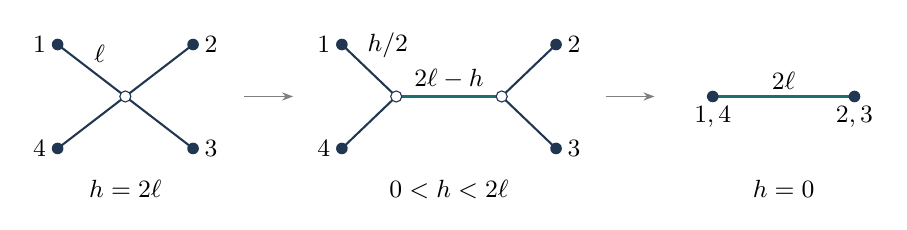
\begin{tikzpicture}[
    x=1cm,y=1cm,
    outer/.style={draw=ink,line width=.75pt},
    trunk/.style={draw=sea,line width=1.15pt},
    site/.style={circle,fill=ink,inner sep=0pt,minimum size=4.2pt},
    branch/.style={circle,draw=ink,fill=white,inner sep=0pt,minimum size=4.0pt},
    lab/.style={font=\small,inner sep=2pt},
    stage/.style={font=\small,anchor=north,inner sep=1pt}
  ]
  \begin{scope}
    \coordinate (p) at (0,0);
    \coordinate (one) at (-.86,.66);
    \coordinate (four) at (-.86,-.66);
    \coordinate (two) at (.86,.66);
    \coordinate (three) at (.86,-.66);
    \draw[outer] (one)--(p)--(two) (four)--(p)--(three);
    \node[lab,above right] at (-.47,.36) {$\ell$};
    \node[branch] at (p) {};
    \foreach \pt/\val/\side in {one/1/left,four/4/left,two/2/right,three/3/right}{
      \node[site] at (\pt) {};
      \node[lab,\side=2pt] at (\pt) {$\val$};
    }
    \node[stage] at (0,-1.02) {$h=2\ell$};
  \end{scope}
  \draw[-{Stealth[length=4pt]},draw=black!50] (1.51,0)--(2.13,0);
  \begin{scope}[shift={(4.11,0)}]
    \coordinate (leftbranch) at (-.67,0);
    \coordinate (rightbranch) at (.67,0);
    \coordinate (one) at (-1.36,.66);
    \coordinate (four) at (-1.36,-.66);
    \coordinate (two) at (1.36,.66);
    \coordinate (three) at (1.36,-.66);
    \draw[outer] (one)--(leftbranch)--(four) (two)--(rightbranch)--(three);
    \draw[trunk] (leftbranch)--(rightbranch);
    \node[lab,above] at (0,.02) {$2\ell-h$};
    \node[lab,above right] at (-1.11,.41) {$h/2$};
    \node[branch] at (leftbranch) {};
    \node[branch] at (rightbranch) {};
    \foreach \pt/\val/\side in {one/1/left,four/4/left,two/2/right,three/3/right}{
      \node[site] at (\pt) {};
      \node[lab,\side=2pt] at (\pt) {$\val$};
    }
    \node[stage] at (0,-1.02) {$0<h<2\ell$};
  \end{scope}
  \draw[-{Stealth[length=4pt]},draw=black!50] (6.10,0)--(6.72,0);
  \begin{scope}[shift={(8.36,0)}]
    \draw[trunk] (-.90,0)--(.90,0) node[lab,midway,above] {$2\ell$};
    \node[site] at (-.90,0) {};
    \node[site] at (.90,0) {};
    \node[lab,below] at (-.90,-.05) {$1,4$};
    \node[lab,below] at (.90,-.05) {$2,3$};
    \node[stage] at (0,-1.02) {$h=0$};
  \end{scope}
\end{tikzpicture}
\caption{第四个尖端与第一个尖端碰撞。在中间的树上，每对内部的距离为 \(h\)，两对中点之间的线段长 \(2\ell-h\)。到最右端时，共享标号成为一条长度为 \(2\ell\) 的连线。}
\label{fig:collision}
\end{figure}

在这三条支臂上，前三个站点各自的深度斜率之和都是 \(-1/2\)，在站点 \(4\) 则为 \(3/2\)。为使所有深度均调和，添加两条长度为 \(\ell\) 的支臂。在一条尚未使用的有限支臂 \(a\in F\setminus\{z_1,z_2,z_3\}\) 上，使每个深度都以 \(1/2\) 的斜率增加。由特殊化，其端点处的归一化价格至多为 \(D_{3\ell/2}\)。在外支臂上取 \(c=t^{-r}u\)。此时只有第四个深度发生变化，斜率为 \(-2\)。当 \(r=\ell\) 时，此站点即为 \(P(0,-\ell)\)。将所得标号的归一化价格记为 \(D_\ell^-\)。沿各射线的价格函数在各自的原点处连续。事实上，对于绝对值小的正负 \(r\)，采用相同的仿射深度规定以及 \(t^r\) 或 \(t^{-r}\)，就可得到跨越零点的凸延拓。

图~\ref{fig:harmonic} 在同一次比较中列出了五条支臂上的深度变化。每列的和都为零，这正是相应站点的调和性条件。

\begin{figure}[htb]
\centering
\begin{tikzpicture}[font=\small,
 inner/.style={draw=ink,line width=.8pt},
 end/.style={inner sep=2pt,anchor=west},
 twig/.style={draw=sea,densely dashed,line width=.85pt},
 up/.style={draw=rust,line width=1.05pt}]
 \draw[inner] (0,0)--(1.9,1.4) node[end] at (1.96,1.4){$z_1$};
 \draw[inner] (0,0)--(2.32,.4) node[end] at (2.38,.4){$z_2$};
 \draw[inner] (0,0)--(2.18,-.9) node[end] at (2.24,-.9){$z_3$};
 \draw[twig] (0,0)--(.48,-1.08);
 \draw[up,{Stealth[length=4pt]}-] (-1.18,0)--(0,0);
 \node at (-1.58,0) {$\infty$};
 \node at (.58,-1.38) {$a$};
 \fill[ink] (0,0) circle (1.8pt);
 \node at (-.19,.36) {$u$};
 \node[anchor=west] at (3.58,0) {$
  \renewcommand{\arraystretch}{1.22}
  \begin{array}{c | c c c c | l}
     &1&2&3&4&\text{端点估计}\\ \hline

    z_1 &1&-1&-1&1& 2\ell\\
    z_2 &-1&1&-1&1& 2\ell\\
    z_3 &-1&-1&1&1& 2\ell\\
    a&1&1&1&1& D_{3\ell/2}\\
    \infty&0&0&0&-4&D_\ell^-
  \end{array}$};
\end{tikzpicture}
\caption{以参数圆盘的一般点 \(u\) 为起点的五条支臂。三条碰撞支臂长均为 \(2\ell\)，未使用的有限支臂 \(a\) 和外支臂的长度均为 \(\ell\)。表中给出四个深度斜率的两倍，以及各端点处标号的归一化价格上界。}
\label{fig:harmonic}
\end{figure}

下面将 \(D_\ell^-\) 与一般的归一化价格比较。从固定的小深度 \(\lambda>0\) 出发，沿外射线走到 \(0<R<\lambda\)，所有长度均取有理数。记归一化价格为 \(D(\lambda,R)\)。以 \(P(0,0)\) 为中心，前三个站点的半径为 \(\lambda\)。由 \eqref{eq:motion-tree}，第四个站点的半径也是 \(\lambda\)，其测地线的前 \(R\) 个单位朝向负深度。将这四个半径同时由 \(\lambda\) 收缩到 \(\ell\le R\)，便得到定义 \(D_\ell^-\) 的放置，故由凸性有
\[
   \frac{D_\ell^-}{2\ell}\le\frac{D(\lambda,R)}{2\lambda}.
\]
先对 \(\ell\) 取上极限，再由射线上的连续性令 \(R\downarrow0\)，最后令 \(\lambda\downarrow0\)，得到 \(\limsup D_\ell^-/(2\ell)\le \underline D\)。将第四个有限端点的上界代入 \eqref{eq:motion-star}，有
\begin{equation}\label{eq:motion-fourstar}
 0\le 3\frac{2\ell-D_\ell}{2\ell}
      +\frac{D_\ell^--D_\ell}{\ell}
      +\frac{D_{3\ell/2}-D_\ell}{\ell}.
\end{equation}
在极限中，三条碰撞支臂的贡献为 \(3(1-\underline D)\)。外支臂的上极限至多是零，而由于 \(D_{3\ell/2}/(3\ell)\to \underline D\)，最后一项趋于 \(\underline D\)。因此 \(0\le 3(1-\underline D)+\underline D\)，即
\begin{equation}\label{eq:motion-upper}
                        \underline D\le 3/2 .
\end{equation}

第~\ref{sec:boundary} 节的矩形比较将用到图~\ref{fig:collision} 中端点 \(h=0\) 附近的这个界。在那里，三个固定尖端组成一副带两条短臂和一条长臂的三脚架。把所得极限价格等式推广到平衡三脚架，得到共享标号的归一化价格 \(8/3\)。该三脚架的三条矩阵乘法连线总长为 \(6\)，故秩比较所得的指数为 \(6/(8/3)=9/4\)。

\section{由共享标签的价格推导下界}\label{sec:boundary}

考虑两个 \(n\) 阶方阵的乘法，把两个输入和输出分别放在三条臂长均为一的三脚架的三个端点。三个矩阵指标各由相距 \(2\) 的两个端点共享，因此乘法张量的价格为 \(6\log n\)。一个秩为 \(r\) 的分解可由三个端点共享的、具有 \(r\) 个取值的标签提供这个张量。若此共享标签的费率为 \(8/3\)，则其价格为 \((8/3)\log r\)，由价格的单调性可得 \(r\ge n^{9/4}\)。我们将在第~\ref{sec:motion}~节构造的族中找到这样的三脚架。先考察一条臂远长于另两条臂时的共享标签费率。以下原理把所得等式推广到三臂等长的情形。

\begin{proposition}[三脚架原理]\label{prop:tripod}
在代数闭域上放置三个站点，使对每一对 \(i\ne j\)，站点间距为 \(a_i+a_j\)，其中 \(a_1,a_2,a_3\ge0\)。其共享标签费率 \(D(a)\) 满足
\[
       D(a)\ \ge\ D_*(a)
       :=a_1+a_2+a_3-\bigl(a_1^{-1}+a_2^{-1}+a_3^{-1}\bigr)^{-1}.
\]
只要有一个 \(a_i=0\)，右侧的倒数项就取零。

现固定谱空间中的三条无限射线，它们构成一个以 \(O\) 为原点的度量三脚架，并假设其价格在径向伸缩下齐次。在 \(D(a)\) 中，把站点 \(i\) 放在射线 \(i\) 上、距 \(O\) 为 \(a_i\) 的位置。若 \(D(a)-D_*(a)\) 在某个正三元组处为零，则它在每个正三元组处都为零。若固定其中两条臂的正长度而让第三条臂趋于无穷时，该差值趋于零，则结论也成立。
\end{proposition}

第一个断言适用于满足指定距离的任意配置。第二个断言比较同一个三脚架上的不同配置。第~\ref{sec:profiles}~至~\ref{sec:contact}~节通过研究多项式乘法的价格如何随次数和系数的位置变化，证明这两个断言。

\subsection{矩形矩阵乘法的解码器}

在第~\ref{sec:motion}~节的代数闭域 \(F\) 上，将一个 \(s\times q\) 矩阵与一个 \(q\times s\) 矩阵相乘。取四次幂 \(N\)，令 \(s=N^{1/2}\)、\(q=N^{1/4}\)。乘积有 \(N\) 个元素。将输出放在 \(A\)，两个输入放在 \(C,D'\)，对应的臂长依次为 \(c,a,b\)。外部指标在 \(AC,AD'\) 上给出大小为 \(s\) 的连线，内部指标在 \(CD'\) 上给出大小为 \(q\) 的连线。因此，将乘积的价格除以 \(\log N\)，所得数满足
\[
   c+\tfrac34(a+b)
   \ \le\ c+a+b-\frac{ab}{a+b}
   \ \le\ D_*(c,a,b)\ \le\ D(c,a,b).
\]
在 \(a=b=0\) 时约定 \(ab/(a+b)=0\)。这就给出了与半宽矩阵乘法对应的矩形界 \cite{uznanski,abvz}。

特别地，对每个 \(\eta>0\)，都有任意大的这种 \(N\)，使精确张量秩至多为 \(N^{1+\eta}\)。事实上，从充分大的四次幂 \(N_0\) 和一个大小为 \(\lceil N_0^{1+\eta/2}\rceil\) 的全对角张量出发。在每个谱点，上述不等式都给出与该对角张量的严格谱比较。乘法张量的每个张量幂都是对应对角张量幂的有界多个副本的限制。幂次充分大时，指数 \(1+\eta\) 足以吸收副本数和取整的影响。

\begin{lemma}[具有短行的解码器]\label{lem:secondary}
对每个 \(\epsilon>0\)，都存在 \(\delta>0\)，使得下述结论对任意大的某些四次幂 \(N\) 成立：这一乘法的 \(N\) 个输出双线性型 \(B_e\) 均有如下分解：
\[
    B_e=S_e+R_e,\qquad
    \operatorname{rank}S_e\le N^\epsilon,\qquad
    \dim\langle R_e:1\le e\le N\rangle\le N^{1-\delta}.
\]
\end{lemma}

这两个界各有用途。共享输出指标 \(e\) 后，每个 \(S_e\) 都可用少量简单乘积的和计算。修正项 \(R_e\) 单独计算可能很昂贵，但它们张成的整个空间可以沿一条连线传输。为得到对基本规格一致的界，我们用一个工作寄存器实现解码器的张量幂。克罗内克积的相关非刚性估计见 \cite{almanrigidity,kivva}。

\begin{proof}
只需考虑 \(0<\epsilon<1\)。固定整数 \(K>10/\epsilon\)。设基本规格有 \(d\) 个输出元素，秩满足 \(d\le r\le d^{1+\eta}\)。令 \(M\) 为把输出表示成 \(r\) 个简单双线性乘积的线性组合的 \(d\times r\) 矩阵。稍后选取 \(\eta\)。第 \(Km\) 个张量幂有 \(N=d^{Km}\) 个输出元素。为每个解码块 \(M^{\otimes m}\) 补上零行和零列，使其成为边长为 \(2^t\) 的方阵，其中 \(t=\lceil m\log_2 r\rceil\)。补零后的整个解码器的边长为 \(T=2^{Kt}\)。每个指标由 \(K\) 个寄存器组成，每个寄存器有 \(t\) 比特。

将第一个块矩阵作用于第一个寄存器。对之后的每一个块，先把其寄存器与第一个交换，在第一个寄存器上施加块矩阵，再交换回来。一次寄存器交换同时交换 \(t\) 对比特。一次比特交换置换四个字母中的两个，即 \(01\) 和 \(10\)。在任意域上，它的矩阵都可分解为固定数目的初等剪切和对角符号变换。因此一次寄存器交换由固定数目的阶段组成，每一阶段在所有比特位置施加同一局部剪切或对角符号变换。

对于剪切，把非对角元素指向的字母称为高位字母。固定一个充分小的 \(\rho>0\)，在该阶段的前后分别作投影，仅保留寄存器对中高位字母的个数介于 \(t/4-\rho t\) 和 \(t/4+\rho t\) 之间的坐标。由二项分布的尾界，当 \(t\) 充分大时，被丢弃的坐标比例至多为 \(e^{-c_\rho t}\)。将 \(O(K)\) 次投影的差逐项作望远镜求和，得到解码器被丢弃部分的秩至多为 \(O(K)Te^{-c_\rho t}\le T^{1-\gamma}\)，其中 \(\gamma=\gamma(K,\rho)>0\)。在剪切阶段被保留的路径上，每一次改变都产生一个高位字母，因此至多有 \(2\rho t\) 个位置发生改变。

块矩阵只作用于第一个寄存器。其他每个寄存器恰参与两次交换，所以在保留的路径上，其输入与输出间的汉明距离至多为 \(C\rho t\)，其中 \(C\) 为绝对常数。因此，保留的解码器的各输出行中，非零元素个数至多为
\[
       2^t\left(\sum_{j\le C\rho t}\binom{t}{j}\right)^{K-1}
       \ \le\ T^{1/K+o_{\rho\downarrow0}(1)}
\]
选取 \(\rho\) 使该指数小于 \(\epsilon/2\)，再取充分小的 \(\eta\)。由于 \(T\le 2^K N^{1+\eta}\)，对一切充分大的 \(m\)，上述两个界分别成为每个保留行至多有 \(N^\epsilon\) 个元素、被丢弃矩阵的秩至多为 \(N^{1-\delta}\)，其中 \(\delta=\gamma/2\)。去掉补上的零行零列，把两个矩阵分别作用于简单双线性乘积的列表。保留下来的行给出双线性型 \(S_e\)，而被丢弃的行空间的像张成 \(R_e\)。
\end{proof}

\subsection{碰撞附近的两个输出副本}

取第~\ref{sec:motion}~节中站点 \(4\) 趋近站点 \(3\) 的碰撞，把站点 \(1,2,3,4\) 分别记为 \(A,B,C,D'\)。在参数 \(r\) 处，记 \(L=2\ell\)、\(h=L-r\)，其中 \(0<h<L\)。\(AB\) 与 \(CD'\) 的内部距离均为 \(h\)，四个跨对距离均为 \(L\)。用 \(D_\ell(h)\) 表示四站点的共享标签费率。碰撞时 \(D_\ell(0)=L\)，而在一般的四站点配置下 \(D_\ell(L)=D_\ell\)。由凸性得到
\[
                   D_\ell(h)\le L+\frac hL(D_\ell-L).
\]

在 \(A\) 和 \(B\) 各放置矩形乘法的输出指标 \(e=(i,i')\) 的一个副本，两个输入仍放在 \(C,D'\)。所得张量为
\[
 U_N=\sum_e e_e\otimes e_e\otimes B_e
     =\sum_{\substack{1\le i,i'\le s\\1\le j\le q}}
        e_{ii'}\otimes e_{ii'}\otimes e_{ij}\otimes e_{ji'} .
\]
指标 \(i\) 由 \(A,B,C\) 共享，指标 \(i'\) 由 \(A,B,D'\) 共享，而 \(j\) 沿短连线 \(CD'\) 传递。以 \(D_{ABC},D_{ABD'}\) 表示两个三元组的费率，则
\[
   \frac{H(U_N)}{\log N}=\frac{D_{ABC}+D_{ABD'}}2+\frac h4 .
\]
两个三元组的臂长均为 \((h/2,h/2,L-h/2)\)。命题~\ref{prop:tripod} 中的倒数修正项至多为 \(h/4\)，故两者的费率均至少为 \(L+h/4\)。

采用引理~\ref{lem:secondary} 的分解 \(B_e=S_e+R_e\)。以 \(\log N\) 为单位，诸 \(S_e\) 形成的张量的成本至多为 \(D_\ell(h)+\epsilon h\)。先在四个站点共享标签 \(e\)，然后在 \(CD'\) 上用一条大小至多为 \(N^\epsilon\) 的连线提供指定 \(e\) 所需的简单乘积。诸 \(R_e\) 形成的张量沿切分 \(AB\mid CD'\) 的矩阵秩至多为 \(N^{1-\delta}\)。用连接 \(A\) 和 \(C\) 的一条连线提供这一秩，再由两对站点各自内部的连线把维数至多为 \(N\) 的张量腿分别送到 \(B\) 和 \(D'\)。这样做的成本至多为 \((1-\delta)L+2h\)。

取 \(h/L<\delta/2\)。此时修正项的成本小于 \(L\)，由限制到一对分属两组的站点可得 \(D_\ell(h)\ge L\)。在固定配置下，对普通和使用价格界只需付出与 \(N\) 无关的加法常数。令 \(N\) 沿引理~\ref{lem:secondary} 的规格趋于无穷，再在固定 \(h/L\) 时应用式~\eqref{eq:motion-upper}，可得
\[
  \frac{D_{ABC}+D_{ABD'}}2+\frac h4
  \ \le\ D_\ell(h)+\epsilon h
  \ \le\ L+\bigl(\tfrac12+\epsilon+o_{\ell\downarrow0}(1)\bigr)h .
\]
减去下界 \(D_{ABD'}\ge L+h/4\) 得
\[
        D_{ABC}\le L+h/4+\bigl(2\epsilon+o_{\ell\downarrow0}(1)\bigr)h.
\]

前三个站点位于从深度为零的点出发的固定射线 \(z_1,z_2,z_3\) 上。为在该点取切三脚架，把站点放在深度 \(t a_i\)，将价格除以 \(t\)，并在谱超极限中令 \(t\downarrow0\)。在这些固定射线上，每个非零张量经缩放的价格都有极限，因为原价格关于 \(t\) 为凸函数且在零处消失。极限价格在径向伸缩下齐次。

令 \(t=h/2\) 并固定 \(b=2L/h-1\)。三个深度变成 \(t(1,1,b)\)。用 \(t\) 除上一个不等式得到 \(D(1,1,b)\le b+3/2+4\epsilon\)，而
\[
             D_*(1,1,b)=b+\tfrac32+\frac{1}{4b+2}.
\]
因此，对一切充分大的有理数 \(b\) 都有 \(0\le D(1,1,b)-D_*(1,1,b)\le4\epsilon\)。由连续性，该式对充分大的实数 \(b\) 也成立。先令 \(b\) 趋于无穷，再令 \(\epsilon\) 趋于零，就得到在这一固定三脚架上无穷远处的接触。命题~\ref{prop:tripod} 现给出 \(D(1,1,1)=3-1/3=8/3\)。本节开头的三连线价格比较随即给出 \(r\ge n^{9/4}\)，从而证明了定理~\ref{thm:motion}。

\section{接触附近的多项式乘法}\label{sec:profiles}

三脚架原理将三个端点的共享标签价格 $D$ 与由臂长 $a_i>0$ 决定的下界 $D_*(a)=\sum_i a_i-(\sum_i a_i^{-1})^{-1}$ 进行比较。我们把取等号的情形称为\emph{接触}，把差值 $\Delta=D-D_*(a)$ 称为缺陷。为将接触推广到其他臂长三元组，我们需要知道仅改变一个输入宽度时价格怎样变化。多项式乘法提供了一个可以测量这种变化的张量。当一个输入增大时，其价格经过指数化后具有极限斜率和截距。命题~\ref{thm:profile-rigidity} 将这些截距确定到误差 $O(\Delta)$。第~\ref{sec:energy}~节接着比较不同配置，第~\ref{sec:contact}~节用这一比较推广等号成立的结论。

在这三节中，基域均为代数闭域，价格取自然对数且距离保持固定。一个由各端点共享、具有 $q$ 个取值的标签，成本为 $D\log q$。在一个嵌入的三脚架上，将原点也纳入共享站点不改变价格。在两个端点中的任一个处添加副本均无须成本，由凸性即可控制在连接二者的测地线上任一点处添加副本的成本。

\subsection{连续极限下的价格函数}
将非空有限个输入和一个输出放在谱空间中。以 $H$ 表示价格，以 $D>0$ 表示该配置的共享标签费率。对整数长度 $L_i\ge1$，以 $M(L)$ 表示将次数分别小于 $L_i$ 的单变量多项式相乘并保留全部输出系数的张量。以下归一化同时确定了下文能量公式中的常数。

\begin{lemma}\label{lem:continuum-profile}
在各坐标均为正的区域上存在一个连续且逐坐标非减的函数 $P$，使得若 $L_i/N\to t_i>0$，则
\[
 H(M(L))=D\log N+P(t)+o(1),\qquad P(ct)=P(t)+D\log c.
\]
对 $m$ 元多项式，若各输入的总次数分别至多为 $\lfloor Nt_i\rfloor$，则对于每个固定的 $m$，相应价格为 $mD\log N+mP(t)-D\log(m!)+o(1)$。
\end{lemma}

\begin{proof}
求值和插值给出 $H(M(L))$ 的上界 $D\log(\sum_iL_i)$。另一方面，$M(kL)$ 退化到 $k$ 个 $M(L)$ 副本的直和。事实上，将 $[0,1]$ 分为 $k$ 个等长区间，取一个连续的凸分段仿射函数，使其在每个内部分点的斜率都严格变化。次数为 $d_i$ 的输入单项式的归一化位置为 $(d_i+1/2)/(kL_i)$。赋予它一个权重，等于 $kL_i$ 乘以函数在该处的值。对于输出，在这些位置的加权平均处取函数值，乘以系数 $k\sum_i L_i$，再反号作为权重。输出权重仅依赖于次数之和。由詹森不等式可知，恰好保留所有输入位于同一区间的项。不同区间使用互不相交的输入和输出坐标，每个留下的块均为 $M(L)$ 的平移副本。权重等式定义了一个有理线性子空间。在该子空间中用有理数逼近可保持有限多个严格不等式，再作缩放即可得到整数权重。因此，对坐标作缩放并利用价格次水平集的闭性，便得到所断言的退化。

对于 $L_i=\lfloor Nt_i\rfloor$，$N$ 处的归一化成本因而不小于任意固定且充分大的 $M$ 处的归一化成本加上误差项 $D\log(M\lfloor N/M\rfloor/N)$。先对 $N$ 取下极限，再对 $M$ 取上极限，即证收敛。改变 $N$ 的单位就得到对数齐次性：先对含取整的尺度作夹逼，再推广到实数 $N$。由逐坐标单调性，在 $(1\pm\epsilon)t$ 之间作夹逼即得连续性，并允许长度有 $o(N)$ 的误差。

对于关于总次数的断言，将输入 $i$ 处的指数向量除以 $Nt_i$，将输出处的指数向量除以 $N\sum_i t_i$。这样各输入都在单位单纯形中的格点上变化。为用超平面切分这个区域，先去掉平面上的输入点。用定义超平面的仿射形式的正部和系数 $Nt_i$，作同样的凸加权。詹森不等式保留各输入均在同侧的项。相应输出也在同侧，故所得两个块构成直和。可在每个块内部重复这种切分。

在一个经平移的、与坐标轴平行且边长为 $s$ 的立方体上，乘法沿 $m$ 个坐标分解为乘积。由单变量极限，其指数化价格除以 $N^m\exp(mP(t)/D)$ 后趋于其体积 $s^m$。平移只需重新标记指数，而将立方体边长取整改变宽度的量是 $O(1)$。由于 $\exp(H/D)$ 对直和可加，用位于单纯形内部的网格立方体填充单纯形，便得到其归一化价格的下界 $1/m!$。为证上界，从一个包围它的立方体出发，切出一个略微放大的单纯形，使所需张量的全部输入点都保留在同一单元中。在其余各单元中填入内部网格立方体。包围立方体的张量控制所需张量与全部填入立方体张量的直和。细化网格并缩小放大量，便可计入补集的全部体积，得到相符的上界 $1/m!$。取对数即得公式。
\end{proof}

\subsection{仅在两个站点可见的标签}

我们还需要对一个和式给出下界，其中的块标签仅在三个站点中的两个处可见。设 $T=\sum_b T_b$，其中 $T_b\ne0$ 且 $T_b\in X\otimes Y_b\otimes Z_b$；诸 $Y_b$ 在 $Y$ 处构成直和，诸 $Z_b$ 在 $Z$ 处构成直和。对块标签上的任一概率分布 $q$，记 $\operatorname{Ent}(q)=-\sum_b q_b\log q_b$，则
\begin{equation}
 H(T)\ge\sum_b q_b H(T_b)+d(Y,Z)\operatorname{Ent}(q).
 \label{eq:pair-entropy}
\end{equation}
为看出熵项的来源，取有理概率分布 $q$ 和幂次 $n$，使所有 $nq_b$ 都是整数。在 $Y$ 和 $Z$ 处保留类型为 $q$ 的 $M=n!/\prod_b(nq_b)!$ 个字。每个字的价格为 $n\sum_bq_bH(T_b)$。将文献~\cite[命题~3.1]{nine} 的共享腿分离法写成文献~\cite[命题~2.1]{lu} 的插值形式，可以把所保留张量的 $2M-1$ 个副本的直和退化为 $M$ 个字块的全直和，其中每个字块都与 $Y,Z$ 上的一条 $M$ 维连线取张量积。插值需要 $2M-1$ 个互不相同的域元素，任一代数闭域均可满足。比较两边的价格得到
\[
 nH(T)+D\log(2M-1)\ \ge\
 n\sum_bq_bH(T_b)+(D+d(Y,Z))\log M ,
\]
其中 $D$ 为三个站点的共享标签费率。又有 $\log((2M-1)/M)\le\log2$ 以及 $n^{-1}\log M\to\operatorname{Ent}(q)$。除以 $n$ 并利用关于 $q$ 的连续性，即得式~\eqref{eq:pair-entropy}。

\subsection{三角形上的斜率与截距}

以 $i,j,k$ 依任意次序标记三个站点，并设各臂长 $a_i$ 均为正。置 $d_i=d(j,k)=a_j+a_k$、$D=\delta(\{i,j,k\})$，以 $P_k(x,y)$ 表示输出位于 $k$、输入在 $i$ 处宽度为 $x$ 且在 $j$ 处宽度为 $y$ 时的连续价格函数。我们以站点来标识相应的自变量。固定第一个输入，定义
\[
 F_{ik}(t)=\exp\bigl(P_k(t_i=1,t_j=t)/d_i\bigr).
\]
多项式乘法的行列式滤过和平移三块退化~\cite[引理~4.1、4.2~的证明]{nine} 给出
\[
 F_{ik}\text{ 为凹函数},\qquad
 F_{ik}(3t+1)\ge 2F_{ik}(t)+F_{ij}(t).
\]
在第一个退化中，$j,k$ 上的一条二维连线提供两个块，$j$ 处的长度在两块中分别增加和减少一。这两个块在该对站点上构成直和。在双站点标签不等式中关于各块的概率作优化，所得相当于将两块在尺度 $d_i$ 下的指数化价格相加。这给出长度格点上的中点凹性，故在极限中得到凹性。在第二个退化中，较长的长度为 $3L_j+L_i-1$，且三个块中的一个交换 $j$ 与 $k$。由同一个双站点标签不等式和引理~\ref{lem:continuum-profile} 得到上式的第二个断言。两种退化都适用于任意特征。对第一种，乘以行列式这一映射的单射性与维数计数给出一次的克莱布施–戈尔丹行列式序列（见~\cite{kowalski}）。只须将单项式提升到该序列的滤过中。第二种使用单项式分次，反转一条腿上的次序即可识别中间的块。

正的递增凹函数在无穷远处具有有限的极限斜率。将三块不等式除以 $t$，可知 $F_{ik}$ 和 $F_{ij}$ 的斜率相等。令 $S=F_{ik}+F_{ij}$，则有 $S(3t+1)\ge3S(t)$。沿 $t_n=3^n(t+1/2)-1/2$ 迭代得到 $S(t)/(t+1/2)\le \lim_{n\to\infty}S(t_n)/(t_n+1/2)$，其右端为公共斜率的两倍。因此该公共斜率为正，将其记为 $\exp(c_i/d_i)$。对这两个函数中的任一个，它与过原点且具有此斜率的直线的差均非负且递增。故由关于 $S$ 的界，存在数 $\beta_{ik},\beta_{ij}\ge0$，满足 $\beta_{ik}+\beta_{ij}\le1$，并有
\[
 t\le e^{-c_i/d_i}F_{ik}(t)\le t+\beta_{ik}.
\]
其中 $\beta_{ik}$ 是将该差除以斜率后所得的极限。特别地，当 $x$ 固定时，$P_k$ 作为 $\log y$ 的函数满足常数为 $d_i$ 的利普希茨条件，因为 $F_{ik}$ 的每个单侧导数均介于零和 $F_{ik}(t)/t$ 之间。

置 $h=(\sum_i1/a_i)^{-1}$、$b_i=a_i-h$、$u_i=b_i/a_i$、$\beta_{ik}^*=a_k/d_i$ 和 $\Delta=D-D_*(a)$，其中 $D_*(a)=\sum_i a_i-h$。由于 $P_k(x,y)=D\log x+P_k(1,y/x)$ 并且 $D-d_i=b_i+\Delta$，截距界给出了对每一对宽度均有效的上包络：
\begin{equation}\label{eq:profile-upper}
 P_k(x,y)\le U_{ik}(x,y):=c_i+(b_i+\Delta)\log x+d_i\log(y+\beta_{ik}x).
\end{equation}

\begin{proposition}[接触附近的连续价格函数]\label{thm:profile-rigidity}
有 $\Delta\ge0$。若 $\min_i u_i\ge\eta>0$，则存在一个对三个站点公共的数 $C$，使
\begin{equation}\label{eq:src2}
 d_i(\beta_{ik}-\beta_{ik}^*)=O_\eta(\Delta),\qquad
 c_i+b_i\log u_i=C+O_\eta(\Delta).
\end{equation}
在扇区 $y/x\ge u_j/u_i$ 内，有
\begin{equation}\label{eq:src3}
 0\le U_{ik}(x,y)-P_k(x,y)\le O_\eta(\Delta).
\end{equation}
\end{proposition}

\begin{proof}
令 $E_{ik}=U_{ik}-P_k$ 和 $z_{ik}=d_i(\beta_{ik}-\beta^*_{ik})$。对 $y$ 求导，并用 $F_{ik}$ 的极限斜率作为其导数的下界，得到
\[
 \partial_y P_k(x,y)\ \ge \frac{d_i}{y+\beta_{ik}x}\exp(E_{ik}(x,y)/d_i).
\]
交换 $i,j$ 可得第二个界。在可微点有 $x\partial_xP_k+y\partial_yP_k=D$。这些函数局部利普希茨，故即使某个导数在 $(x,y)=(u_i,u_j)$ 处不存在，仍可利用连续性在该点给出两个导数界之和。在该点有 $u_j+u_i\beta^*_{ik}=1$ 和 $u_jd_i+u_id_j=D_*$。对 $r=u_i z_{ik}/d_i$ 使用 $(1+r)^{-1}=1-r+r^2/(1+r)$，并对 $s\ge0$ 使用 $e^s\ge1+s$。由于 $\eta\le u_j+u_i\beta_{ik}\le2$，存在 $c_\eta>0$，使得
\[
 \frac{\Delta}{u_iu_j}\ge -(z_{ik}+z_{jk})+
 c_\eta\left(E_{ik}+E_{jk}
           +\frac{z_{ik}^2}{d_i}+\frac{z_{jk}^2}{d_j}\right),
\]
其中所有差值均取在指定宽度处。由于 $\beta^*_{ik}+\beta^*_{ij}=1$，各行和 $z_{ik}+z_{ij}$ 均非正。对所有输出站点 $k$ 求和得到 $\Delta\ge0$，且每一个非负余项均以 $O_\eta(\Delta)$ 为界。因此每个行和介于 $-O_\eta(\Delta)$ 和零之间。由上式，每一列的和至少为 $-O_\eta(\Delta)$。由于各列的总和等于各行的总和，每个列和也至多为 $O_\eta(\Delta)$。

现比较 $P_k(u_i,u_j)$ 的两个包络，得到
\[
 c_i+b_i\log u_i+u_i z_{ik}
 =c_j+b_j\log u_j+u_j z_{jk}+O_\eta(\Delta).
\]
其中对数的泰勒余项由 $z_{ik}^2/d_i$ 和 $z_{jk}^2/d_j$ 控制。由行、列估计可知，在相差 $O_\eta(\Delta)$ 的意义下，各项 $(z_{12},z_{13},z_{23},z_{21},z_{31},z_{32})$ 依次交替取值 $z_{12}$ 和 $-z_{12}$。将对应于 $(i,j)=(1,2),(2,3),(3,1)$ 的三个包络比较式相加，诸项 $c_i+b_i\log u_i$ 抵消，余下 $2(u_1+u_2+u_3)z_{12}=O_\eta(\Delta)$。这证明了式~\eqref{eq:src2}。差值 $E_{ik}$ 仅依赖于 $y/x$。$t+\beta_{ik}$ 与 $e^{-c_i/d_i}F_{ik}(t)$ 的差随 $t$ 递减，而后一个函数递增。因此两者之比的对数递减，从而证明式~\eqref{eq:src3}。
\end{proof}

例如，在单位三脚架上出现接触时，预期的截距为 $\beta^*_{ik}=1/2$，且 $u_i=u_j=2/3$。因此，对 $t\ge1$ 有 $e^{-c_i/d_i}F_{ik}(t)=t+1/2$。更一般地，当一条臂趋于无穷而其他两条臂的长度仍在 $(0,\infty)$ 的一个紧子集中时，式~\eqref{eq:src2} 中的估计仍然一致。若一条臂的长度为零，则由直径界得到 $D\ge D_*(a)$。

\section{能量与径向收缩}\label{sec:energy}

固定一个输出及一个由非空有限个输入组成的集合 $A$，所有端点的共享标签费率为 $D>0$。若每单位输入宽度的成本为 $\ell_i>0$，定义能量
\begin{equation}\label{eq:energy-widths}
 Q_A(\ell)=D+\sup_{t_i>0}\bigl(P(t)-\ell\cdot t\bigr).
\end{equation}
由求值界可知，它取有限值，关于 $\ell$ 为凸函数，并由 $P$ 的对数齐次性满足 $Q_A(c\ell)=Q_A(\ell)-D\log c$。加上公共附加费 $s$，相当于对一个候选宽度向量加上 $s\sum_i t_i$ 的惩罚。因此，最优能量沿成本共同增加方向的斜率度量了总宽度。我们要用到有限差 $Q_A(\ell)-Q_A(\ell+s\mathbf1)$。引理~\ref{lem:energy-compare} 表明，当各输入移向输出，且各自的成本成比例减少时，该能量降幅只能减小。我们先对齐次多项式的次数证明这一比较；在该情形下可以把一个输入从一次多项式乘法转移到另一次乘法；再对这些次数进行缩放，恢复 $Q_A$。

为比较不同配置，先对齐次多项式的每单位次数收取成本 $f_i>0$。记 $M_m^{\mathrm{hom}}(r)$ 为 $m$ 元齐次多项式的乘法，输入次数为 $r=(r_i)_{i\in A}$。定义
\[
 B_A(f)=\sup_{m\ge1,\ r_i\in\mathbb Z_{\ge0}}
 \frac{H(M_m^{\mathrm{hom}}(r))-\sum_i f_i r_i}{m}.
\]
此量有限。用输出空间的对偶空间中由求值泛函组成的一组基进行求值和插值，可知秩至多为输出空间的维数。令 $R=\sum_i r_i$、$q=\exp(-\min_i f_i/D)$，则扣除成本后的价格在尺度 $D$ 下的指数值至多为 $\binom{m-1+R}{R}q^R\le(1-q)^{-m}$。若要求 $m$ 是指定整数的倍数，上确界仍不变。事实上，取互不相交的变量组，原张量的任意次幂都可由次数合并后的乘法经限制得到。

\begin{lemma}[添加一个输入]\label{lem:increasing-returns}
若 $\varnothing\ne A'\subseteq A$ 且 $s>0$，则
\begin{equation}\label{eq:src5}
 B_A(f)-B_A(f+s\mathbf1)\ge
 B_{A'}(f)-B_{A'}(f+s\mathbf1),
\end{equation}
其中成本分别限制在相应的输入集上。如果限制后配置中的所有站点重合，则其能量为零。
\end{lemma}

\begin{proof}
只需添加一个输入 $e$。将待证式改写为右边等于 $B_{A'}(f)+B_A(f+s\mathbf1)$ 的形式，并选择两次乘法分别逼近这两个上确界。通过在分开的变量组上取幂，可以使两者使用同一数目 $m$ 的变量。将其变量分别记为 $u=(u_1,\ldots,u_m)$ 和 $v=(v_1,\ldots,v_m)$。在每个公共输入处，这两次乘法的张量积接收关于 $(u,v)$ 的、具有指定双次数的双齐次多项式。在 $e$ 处，它接收次数为 $q$ 的多项式 $h(v)$。记包含 $q$ 在内的总双次数为 $(U,V)$。

我们将这个张量积实现为若干乘法的和，其中 $e$ 改属于 $u$ 变量组。将 $h(v)$ 改记为 $h(u)$，并在公共输入处以 $u-v$ 替换 $u$。相乘后，在输出处以 $u+v$ 替换 $u$，再投影到双次数 $(U,V)$。对公共输入所作的两次代换相互抵消，且 $h(u+v)$ 中在投影后保留的项只有 $h(v)$。该恒等式不涉及除法。在相乘前将中间输入按双次数展开。如果公共输入总共有 $k$ 个单位次数从 $u$ 转到 $v$，则中间的 $v$ 次数为 $V-q+k$。最后的代换只会增大这个次数，因此能被保留的分块必有 $k\le q$。每个输入处的总次数不变。因此，每个分块的基本成本不变，其在 $v$ 上的附加费至多为 $sV$。每个分块都可分解为含全部输入的 $u$ 变量乘法与含输入 $A'$ 的 $v$ 变量乘法，再加上局部的预处理和后处理。

将这一构造用于各变量组有 $nm$ 个变量的幂，并将所有次数乘以 $n$。由于 $A$ 固定，双次数分块的数目关于 $n$ 至多按多项式增长。普通和的价格界仅比最大分块价格多 $O(\log n)$。除以 $nm$ 再取极限，右侧便以 $B_A(f)+B_{A'}(f+s\mathbf1)$ 为界，结论得证。
\end{proof}

\subsection{从次数到宽度}

每单位次数收费 $\ell_i/N$，就使 $N$ 量级的次数对应于常数量级的宽度。引理~\ref{lem:continuum-profile} 中对总次数受限多项式出现的因子 $1/m!$，解释了式~\eqref{eq:energy-widths} 中的加法常数 $D$。

\begin{lemma}[次数能量的连续极限]\label{lem:continuum-energy}
对共享标签费率为 $D>0$ 的配置，有
\begin{equation}\label{eq:src6}
 B_A(\ell/N)=D\log N+Q_A(\ell)+o(1)
 \qquad(N\longrightarrow\infty).
\end{equation}
\end{lemma}

\begin{proof}
以 $S_m(r)$ 表示各输入总次数分别\emph{至多}为 $r_i$ 的多项式乘法。用其价格减去次数成本后除以 $m$，得到 $B_A$ 的一个下界。事实上，在互不相交的变量组上取 $n$ 个副本，可由 $nm+1$ 个变量、次数为 $nr_i$ 的齐次乘法经限制得到：用最后一个变量作齐次化，再在输出处令其为一。因此 $B_A(f)\ge n(H(S_m(r))-f\cdot r)/(nm+1)$，再令 $n\to\infty$。取 $r_i=\lfloor Nm t_i\rfloor$，引理~\ref{lem:continuum-profile} 给出
\[
 \liminf_{N\to\infty}(B_A(\ell/N)-D\log N)
 \ge P(t)-\ell\cdot t+D\bigl(\log m-m^{-1}\log(m!)\bigr).
\]
最后一项趋于 $D$。对 $t$ 取上确界即得所需下界。

为证上界，取整数 $N$。在定义 $B_A$ 的上确界中可使用 $Km$ 个变量，将它们分成 $K$ 组，每组 $m$ 个。在每个输入处，通过分箱 $[(b_i-1)N,b_iN)$（$b_i\ge1$）记录各组变量的总次数。对固定的分箱模式，相应的乘法可以由各组的 $S_m(Nb)$ 的乘积经限制得到，而每组的成本至少为 $\sum_i\ell_i(b_i-1)$。对各模式求和所得的价格，以各自价格在尺度 $D$ 下取指数、求和再取相应对数后的结果为界。各组独立地对所有箱求和，可将该和放大成一个 $K$ 次幂。对其取对数，除以 $Km$ 并取上确界，得
\[
 B_A(\ell/N)\le \frac Dm\log\sum_{b\in\mathbb Z_{>0}^A}
 \exp\left(\frac{H(S_m(Nb))-\sum_i\ell_i(b_i-1)}{D}\right).
\]
固定 $m$，从和式提出因子 $N^m$ 后，由输出维数的界，各项均由某个常数乘以 $(m+\sum b_i)^m\exp(-\ell\cdot b/D)$ 控制。利用引理~\ref{lem:continuum-profile} 和控制收敛定理，得到 $B_A(\ell/N)-D\log N$ 的上极限至多为
\[
 D\left(\log m-\frac{\log(m!)}m\right)
 +\frac{\sum_i\ell_i}m+
 \frac Dm\log\sum_b\exp\left(\frac{mP(b/m)-\ell\cdot b}{D}\right).
\]
对于 $0<\epsilon<1$，用 $P(t)-(1-\epsilon)\ell\cdot t$ 的上确界估计最后一项，余项至多为 $(D/m)\log\sum_b\exp(-\epsilon\ell\cdot b/D)$。先令 $m\to\infty$，再令 $\epsilon\downarrow0$，并应用 $Q_A$ 的尺度变换关系。由关于 $N$ 的单调性，在实数尺度下也得到相同极限。
\end{proof}

\begin{lemma}[径向收缩]\label{lem:energy-compare}
将每个输入 $i$ 沿其通向输出的测地线移动，使它距输出的距离为原距离的 $0<\lambda_i\le1$ 倍。以 $A'$ 表示所得配置，并令 $\ell'_i=\lambda_i\ell_i$。对于 $s>0$，若两个配置的共享标签费率均为正，则有
\begin{equation}\label{eq:src7}
 Q_A(\ell)-Q_A(\ell+s\mathbf1)\ge
 Q_{A'}(\ell')-Q_{A'}(\ell'+s\mathbf1)
\end{equation}
\end{lemma}

\begin{proof}
在某个输入自身的站点处以相同成本复制该输入，可以作局部乘法，因而 $B$ 不变。同样，在输出处以零成本添加一个输入，可以在输出处作局部乘法，因而 $B$ 不变。在这两个断言中，取新增输入的次数为零就给出反向不等式。对于每个固定的多重次数，随着新增输入沿测地线移动，价格是凸函数，被扣除的成本则为仿射函数。因此，若新增输入的径向距离比例为 $\lambda_i$、成本至少为 $\lambda_i f_i$，则 $B$ 不变。先添加一个，再逐个添加，即得对所有新增输入的结论。该论证既适用于 $f=\ell/N$，也适用于将每项成本增加 $s/N$ 之后的情形，因为 $\lambda_i\ell_i+s\ge
\lambda_i(\ell_i+s)$。以规定的成本插入各移动后的输入，利用引理~\ref{lem:increasing-returns} 删除原来的输入。所得配置的能量降幅以原配置的能量降幅为界。在式~\eqref{eq:src6} 中令 $N\to\infty$。首项 $D\log N$ 在每个配置中分别抵消，因而证明了式~\eqref{eq:src7}。
\end{proof}

\section{等号在三脚架上的传播}\label{sec:contact}

固定三条无限射线，它们构成以 $O$ 为原点的度量三脚架。这些射线上的价格在同时作径向伸缩时是齐次的。对臂长为 $a_1,a_2,a_3$ 的三个端点，命题~\ref{thm:profile-rigidity} 给出 $D(a)\ge D_*(a)$。现在证明命题~\ref{prop:tripod} 的刚性断言：只要在一个臂长三元组处取等号，就必然在每一个三元组处都取等号。若固定其中两条臂的正长度，而第三条臂的长度趋于无穷时渐近地取到等号，也有同样的结论。

取长度的倒数作为坐标：
\[
 v_i=1/a_i,\qquad h(a)=\frac{1}{v_1+v_2+v_3},\qquad
 \Delta(v)=D(a)-D_*(a).
\]
一条无穷长臂现在对应于一个坐标面。我们先比较缺陷沿从 $v$ 出发的三条坐标射线的积分。在 $\Delta$ 的一个零点处，这些积分相等。径向齐次性继而迫使其公共值为零。

\subsection{比较三个方向的积分}

由连续价格函数给出的下界及经过 $O$ 的生成树可得 $D_*(a)\le D(a)\le\sum_i a_i$。等价地，
\begin{equation}\label{eq:defectbound}
 0\le \Delta(v)\le\frac{1}{v_1+v_2+v_3},\qquad
 \Delta(rv)=r^{-1}\Delta(v)\quad(r>0).
\end{equation}
在各坐标均为正的区域上，$\Delta$ 局部利普希茨且局部半凸。半凸是指，对于给定的小球，存在适当的 $C$，加上 $C|v|^2$ 后函数在小球上为凸函数。事实上，由联合测地凸性，$D$ 关于臂长为凸函数。将单个端点移动距离 $t$，$D$ 的改变量至多为 $t$。变量替换 $a_i=1/v_i$ 在内部的紧集上具有有界的一、二阶导数，且 $D_*$ 在其中光滑。

当 $v_1\downarrow0$ 时，由同一传输界，函数 $D(a)-\sum_i a_i$ 非增，并以 $-h(a)$ 为下界。由于 $h(a)$ 在此也有极限，$\Delta$ 可延拓到开面 $v_1=0$。当另外两个变量在 $(0,\infty)$ 的紧子集内变化时，关于它们的利普希茨常数和半凸性常数可一致选取，包括 $v_1\downarrow0$ 的情形。因此上述延拓连续，且具有相同的切向正则性。其余各面只须重新编号即可处理。

对每个内点 $v$ 及坐标向量 $e_i$，置
\[
 J_i(v)=\int_0^\infty
 \left[\Delta(v+t e_i)-\mathbf 1_{\{t\le1\}}\Delta(v)\right]
       \frac{dt}{t}.
\]
由局部利普希茨连续性，减去的项使积分在零处收敛。式~\eqref{eq:defectbound} 保证在无穷远处收敛。我们将证明估计
\begin{equation}\label{eq:src10}
                   |J_i(v)-J_j(v)|\le C\Delta(v).
\end{equation}
其中 $C$ 直至每个开面均局部一致。在一个面上，对该面的两个切向方向也有相同估计。

\paragraph{能量的一个导数。}
固定 $v$，以 $a_i=1/v_i$ 为三个输入端点的位置，将输出置于 $O$。记式~\eqref{eq:energy-widths} 中相应的能量为 $Q$。对变量 $s\in(0,\infty)^3$，置
\[
 G_v(s)=Q\big((a_i s_i)_i\big)+\sum_i a_i\log s_i
                   -h(a)\log\Big(\sum_i s_i\Big).
\]
将 $s$ 沿 $v$ 方向移动，会使每一项成本 $a_i s_i$ 均以单位速率增加。在同一三脚架上，将端点 $i$ 置于距原点 $r/s_i$ 处，且每个输入的成本均为 $r$。在臂 $i$ 上，成本与距离之比仍为 $s_i$。对于小的 $r$，比较配置位于固定配置之内；对于大的 $r$，则位于其外。由引理~\ref{lem:energy-compare}，内、外配置的能量降幅分别从下、上两个方向给出固定配置降幅的界。

在比较配置处，共享标签费率为 $rD((1/s_i)_i)$。将 $O$ 加入原来的三个标签站点无需额外成本。因此，由 $Q$ 的尺度变换律，将所有成本由 $r$ 提高到 $r+t$ 会使能量降低 $rD((1/s_i)_i)\log(1+t/r)$。除以 $t$ 后，当 $t\downarrow0$ 时，上、下界均趋于 $D((1/s_i)_i)$。对 $G_v$ 中两个显式对数项求导，会增加 $\sum_i1/s_i-1/\sum_i s_i=D_*((1/s_i)_i)$。因此
\begin{equation}\label{eq:src8}
       \left.\frac{d}{dt}\right|_{t=0+}G_v(s+tv)=-\Delta(s).
\end{equation}
有限值凸函数 $Q$ 局部利普希茨，因此这一恒等式可以沿 $v$ 方向的任意射线积分。

\paragraph{从坐标轴附近出发的射线。}
令 $s_i=1$、$s_j=s_k=\varepsilon$。回顾第~\ref{sec:profiles}~节中的 $b_i=a_i-h(a)$ 以及截距 $c_i$。记 $B_i=b_i+\Delta(v)$、$d_i=a_j+a_k$。$G_v$ 的极限为
\begin{equation}\label{eq:src9}
           \lim_{\varepsilon\downarrow0}G_v(s)
                =c_i+B_i\log\frac{B_i}{a_i}.
\end{equation}
为证上界，设三个输入宽度为 $x,t_j,t_k$，并将输出位于 $O$ 时的连续价格函数记为 $P(x,t_j,t_k)$。点 $O$ 将从 $j$ 到 $k$ 的线段按 $a_j:a_k$ 分割。由关于输出位置的凸性，$P$ 不超过输出分别位于 $k$ 和 $j$ 时两个函数的加权平均，权重分别为 $a_j/d_i$ 和 $a_k/d_i$。在任一端点处，位于输出站点的输入可通过局部乘法并入。由式~\eqref{eq:profile-upper} 和 $\beta_{ik},\beta_{ij}\le1$ 得
\[
 P(x,t_j,t_k)\le c_i+B_i\log x
                +a_j\log(t_j+x)+a_k\log(t_k+x).
\]
在能量公式中取成本 $(a_i,\varepsilon a_j,\varepsilon a_k)$。将变量换为 $x,t_j+x,t_k+x$，使得当 $\varepsilon$ 较小时，$x$ 的有效成本等于 $a_i-\varepsilon d_i>0$。分别对三项取最大值，并利用 $B_i+d_i=D(a)$，得
\[
 Q\le c_i+B_i\log\frac{B_i}{a_i-\varepsilon d_i}
                  +d_i\log(1/\varepsilon).
\]

为得出相符的下界，取 $x=B_i/a_i$、$t_j=1/\varepsilon$、$t_k=x+t_j$。在 $O$ 处抽取乘积的单个系数。选取互补的次数并反转 $k$ 处的基的次序，就可把此系数写成第三个输入与前两个输入的乘积的配对。端点相差一的取整不改变连续价格函数。因此 $P(x,t_j,t_k)\ge P_k(x,t_j)$，由第~\ref{sec:profiles}~节的渐近斜率知
\[
       P_k(x,t_j)=c_i+B_i\log x+d_i\log(1/\varepsilon)+o(1).
\]
这样选取的总宽度成本趋于 $B_i+d_i=D(a)$，恰好抵消能量公式中的加法常数。利用 $G_v$ 中的对数项减去 $d_i\log(1/\varepsilon)$，就得到式~\eqref{eq:src9}。

\paragraph{通过积分作比较。}
从 $e_i$ 和 $e_j$ 附近分别引出两条射线，其起点取式~\eqref{eq:src9} 中所用的形式。在两条射线上沿 $v$ 方向对式~\eqref{eq:src8} 积分，再相减。由于 $G_v(rs)=G_v(s)-\Delta(v)\log r$ 且 $G_v$ 在 $v$ 处连续，两条射线末端的 $G_v$ 值之差在无穷远处趋于零。现令两个起点分别趋于 $e_i$ 和 $e_j$。由式~\eqref{eq:defectbound}，两个被积函数在零附近一致有界。由齐次性及 $v$ 附近的利普希茨界，它们在无穷远处的差为 $O(t^{-2})$。因此，式~\eqref{eq:src9} 中两个坐标轴极限之差等于
\[
 \int_0^\infty\big[\Delta(e_i+tv)-\Delta(e_j+tv)\big]\,dt
    =J_i(v)-J_j(v).
\]
最后一个恒等式用到了 $\Delta(e_i+tv)=t^{-1}\Delta(v+t^{-1}e_i)$ 及代换 $u=1/t$。

由式~\eqref{eq:src2}，诸量 $c_i+b_i\log(b_i/a_i)$ 之差为 $O(\Delta(v))$。将 $b_i$ 替换为 $B_i$ 也只使每一项改变 $O(\Delta(v))$。事实上，当另外两条臂长的倒数保持在 $(0,\infty)$ 的紧子集中且 $v_i$ 趋于零时，$b_i/a_i$ 有与零隔开的正下界。更一般地，在每个开面上的每一点附近，三个比值都有与零隔开的正下界。由式~\eqref{eq:defectbound} 另有 $B_i/a_i\le1$。因此在所考察的区间内，函数 $b\mapsto b\log(b/a_i)$ 的导数一致有界。这就证明了具有所述一致性的式~\eqref{eq:src10}。在一个面的两个切向方向上，由零处的切向利普希茨界和无穷远处的式~\eqref{eq:defectbound} 可应用控制收敛定理。

\subsection{强极小值原理}

\begin{proof}[命题~\ref{prop:tripod} 的证明续完]
假设 $\Delta(v)=0$。在内部或在一个开面上讨论，只考虑正坐标，重新编号为 $1,\ldots,k$。由式~\eqref{eq:src10}，所有 $J_i(v)$ 都等于同一个 $J\ge0$。同时伸缩所有坐标，可得精确的变化关系 $J_i((1+\varepsilon)v)=J/(1+\varepsilon)$。为将这一降幅与各射线上的变化比较，将伸缩改为逐坐标进行，其中间点为
\[
          v^i=v+\varepsilon\sum_{j\le i}v_j e_j
               \qquad(0\le i\le k).
\]
在每个中间点，从 $J_i$ 换为 $J_{i+1}$ 的误差以 $C\Delta(v^i)$ 为界。因此
\[
 S_\varepsilon=\sum_{i=1}^k\big(J_i(v^i)-J_i(v^{i-1})\big)
   =\frac{J}{1+\varepsilon}-J+
                  O\!\left(\max_{0<i<k}\Delta(v^i)\right).
\]
记 $K=\limsup_{\varepsilon\downarrow0}
\max_{0<i<k}\Delta(v^i)/\varepsilon$，它由局部利普希茨连续性可知是有限的，并置 $g_i(t)=\Delta(v+te_i)$。我们断言
\begin{equation}\label{eq:src11}
 -J+CK\ \ge\ \liminf_{\varepsilon\downarrow0}
              \frac{S_\varepsilon}{\varepsilon}
        \ \ge\ \sum_{i=1}^k v_i\int_0^\infty g_i'(t)\,\frac{dt}{t}.
\end{equation}

为证明第二个不等式，在所有 $k$ 个积分中使用同一变量 $t$。对几乎所有 $t>0$，$\Delta$ 在 $[v^{i-1}+te_i,v^i+te_i]$ 上的增量除以 $\varepsilon$ 后趋于 $v_i g_i'(t)$。事实上，加上一个局部二次函数后，该线段上的斜率介于沿 $e_i$ 方向、以任意固定小长度取得的相邻线段的斜率之间。令 $\varepsilon$ 趋于零，再在 $g_i$ 可微的每一点处缩短相邻线段。对于 $t\le1$ 而减去的未平移增量，其和为 $\Delta((1+\varepsilon)v)-\Delta(v)=0$。

这些被减去的项也控制了零处的奇性。将每个平移后的增量与其未平移的增量配对。由于两线段长度和方向相同，加上一个局部二次函数后，平移后的增量不小于未平移的增量。减去这一二次函数，得到差值的下界 $-C\varepsilon t$。当 $t$ 很大时，将起点移动 $\varepsilon v_i e_i$，会使相应臂长改变 $O(\varepsilon t^{-2})$。用传输可控制 $D$ 的改变量，由 $D_*$ 的公式可得相同的界。除以 $\varepsilon t$ 后，这些界一致控制负部。在一个面上，可对切向变量作相同估计。由法图引理，式~\eqref{eq:src11} 得证。每个极限积分的负部均有限，因为 $g_i$ 在零附近半凸且在零处取最小值。

右导数 $g_i'(0+)$ 存在且非负。如果某个右导数为正，那么由半凸性，$g_i'$ 在零附近有正下界，从而式~\eqref{eq:src11} 中的相应积分发散到正无穷。因此每个 $g_i'(0+)$ 都为零。由半凸性，$\Delta$ 在 $v$ 处的方向导数作为方向的函数是次线性的；又因该点为极小值点，方向导数非负。它在各个正坐标向量上为零，因此在这些向量的正锥上都为零。特别地，$K=0$。分部积分得到
\[
       -J\ \ge\ \sum_{i=1}^k v_i
                    \int_0^\infty\frac{g_i(t)}{t^2}\,dt\ \ge\ 0.
\]
因为在零处有 $g_i(t)=o(t)$，而在无穷远处有式~\eqref{eq:defectbound}，故边界项消失。由于 $J\ge0$，连续性给出对每个 $i$ 和 $t\ge0$ 都有 $g_i(t)=0$。依次沿各条坐标射线使用相同论证，可到达逐坐标不小于 $v$ 的任意一点。任一正三元组，或同一开面上的任一点，都可以通过伸缩进入这一区域。于是，由齐次性，缺陷在最初所在的整个内部或整个开面上为零。

最后还需把一个面上的零点移到内部。设 $v_1=0$ 且 $\Delta(v)=0$。在 $v^{(r)}=v+re_1$ 处，切向控制收敛给出 $J_2(v^{(r)})\to J_2(v)=0$。由一致估计式~\eqref{eq:src10} 及 $\Delta$ 的连续性，同样有 $J_1(v^{(r)})\to0$。虽然在面上只有切向利普希茨界，但由传输可知 $\Delta-h=D-\sum_i a_i$ 关于 $v_1$ 非减。由于 $h$ 的法向导数在该点附近有界，
\[
 \Delta(v^{(r)}+te_1)-\Delta(v^{(r)})\ge-Ct \qquad(0<t\le1).
\]
在法向积分中应用法图引理，得到 $\int_0^\infty\Delta(v+te_1)\,dt/t\le0$。连续且非负的被积函数在每个 $t>0$ 处均为零，给出了上文所需的内部零点。特别地，在上述任一情形下发生接触的齐次三脚架都满足 $D(1,1,1)=3-1/3=8/3$，这就是第~\ref{sec:boundary}~节所用的等臂值。
\end{proof}

\subsection{价格取最大值时的三条连线长度}

命题~\ref{prop:tripod} 中无条件成立的不等式给出了已知方阵上界的一个几何证明，并确定了取等号时连线的价格。在三个站点上取尺度一，因而三者共享的标签费率为一。对 \(i\ne j\)，将三条连线的长度分别写作 \(a_i+a_j\)。由三角不等式，\(a_i\ge0\)。在代数闭域上，上述命题与算术平均数–调和平均数不等式给出
\begin{equation}\label{eq:arm-perimeter}
  1\ \ge\ \sum_i a_i-\Big(\sum_i a_i^{-1}\Big)^{-1}
     \ \ge\ \frac89\sum_i a_i .
\end{equation}
若有一条臂长度为零，式中的倒数项取零。转到代数闭包时三条连线的联合取值保持不变（第~\ref{sec:prices-background}~节），所以同样的界对任意域都成立。由于 \(T_n\) 在每一边上由一条 \(n\) 维连线构成，每个谱点赋予它的值为 \(n^{2\sum_i a_i}\le n^{9/4}\)。由Strassen 关于渐近秩的最大值公式~\cite{spectrum}，即得上界。再如引理~\ref{lem:specialize} 中那样作固定规模的递归，就得到 \(\omega_F\le9/4\)。

\begin{corollary}\label{cor:extremal-price}
固定 \(n\ge2\) 及域 \(F\)。在每个使 \(T_n\) 的值达到最大的尺度一谱点，三条连线的长度全都为 \(3/4\)。这样的谱点存在，而且对于任意正整数 \(a,b,c\)，它赋予 \(T_{a,b,c}\) 的值均为 \((abc)^{3/4}\)。
\end{corollary}

\begin{proof}
谱最大值可以达到。推论~\ref{cor:tight} 确定其值为 \(n^{9/4}\)，因此 \(\sum_i a_i=9/8\)。式~\eqref{eq:arm-perimeter} 中的两个不等式都必须取等号。三条臂的长度都为正，因为若有一条为零，就会得到 \(1\ge9/8\)。算术平均数等于调和平均数给出对每个 \(i\) 均有 \(a_i=3/8\)。因此每条连线的费率都是 \(3/4\)。矩形张量具有三条维数分别为 \(a,b,c\) 的连线，其值等于三者的值之积。
\end{proof}

\section{张量参数的同步}\label{sec:sync}

定理~\ref{thm:extension} 给出了判定同一价格延拓是否适用于整个族的检验。检验时可以任选族中的若干张量，将其相乘，再联合闭合其额外的腿。对于依赖某个标记点 $s$ 的族，这种检验中的两个因子因而可以具有不同的标记点。第~\ref{sec:sphere}~节对球面所作的计算，将给出所有因子使用同一标记点时的估计。我们证明，只要方阵乘法的指数严格小于九分之四，这种对角检验就足以控制标记点的任意选择。

固定一个代数闭域 $F$、基础站点集 $S$ 上尺度为 $D>0$ 的普通价格 $H$，以及称为开口的额外站点组成的有限集 $L$。回顾式~\eqref{eq:prices-beta}，$\beta_H$ 度量的是取张量幂后在每个开口施加一个联合泛函时，每个副本所能取得的最大价格。对于多项式张量族 $T(\mathbf s)$（其中 $\mathbf s=(s_1,\ldots,s_d)$），记
\[
 \beta_H^{\rm gen}(T(\mathbf s))
    =\sup_{\mathbf c\in F^d}\beta_H(T(\mathbf c)).
\]
对于第~\ref{sec:valued}~节中 $H$ 的一般延拓，这就是在相互独立的不定元处的辅助成本。事实上，固定一个幂次和一个系数为有理函数的闭合操作。可以在某个公共开集上同时对其元素和张量作特殊化，使所得价格任意接近一般值。反之，若 $F$ 上的一个固定闭合操作在一点处验证了某个严格下界，由价格次水平集的闭性，它也在某个非空开集上验证同一个界。因此，将参数域限制到任意稠密开集都不改变上确界。

\begin{theorem}[同步]\label{thm:sync}
假设 $\omega_F<9/4$。对于 $F^d$ 上具有相同基础站点和开口的任意多项式张量族 $U_1,\ldots,U_a$，有
\[
 \beta_H^{\rm gen}\!\left(\bigotimes_{i=1}^a U_i(\mathbf s_i)\right)
 =
 \beta_H^{\rm gen}\!\left(\bigotimes_{i=1}^a U_i(\mathbf s)\right).
\]
左侧的 $a$ 个参数向量独立变化，右侧的参数向量则全部相等。两侧的乘积都在每个开口将张量腿归为一组，因此任一侧的闭合操作都可以将所有因子耦合起来。
\end{theorem}

\begin{proof}
选取相同参数便得到右侧不大于左侧。为证反向不等式，先考虑同一单变量族 $U(s)$ 的多个副本。若有一个因子恒为零，断言立即成立，因此可以假设所考虑的族都非零。记 $B=\beta_H^{\rm gen}(U(s))$。由张量幂的齐次性，$a$ 个副本的对角成本为 $aB$。我们先控制同一剩余类 $s$ 上方的一个圆盘内的不同参数，再令该圆盘的赋值深度趋于零以恢复独立参数。

\smallskip\noindent\emph{在同一剩余类上方钉扎站点。}
取不可数个独立不定元组成的集合 $\mathcal U$，另取一个不定元 $s$。置
\[
 E=F(\mathcal U,s),\qquad
 K_0=\operatorname{Frac}(F(\mathcal U)[t^{\mathbb Q}]),\qquad
 J=\{z\in K_0:\nu(z)>0\}.
\]
将 $H$ 一般延拓到 $E$ 后再作高斯提升，所得为 $K_0(s)$ 上的赋值价格 $p$（定理~\ref{thm:gauss}）。对于 $z\in J$，平移 $z$ 保持单位圆盘不变。对该平移及其逆施用引理~\ref{lem:star}，并取 $s$ 为新的剩余变量，得到
\begin{equation}\label{eq:sync-disk-single}
     \beta_p(U(s+z))=\beta_p(U(s))=B .
\end{equation}
第二个等号成立，是因为对于与 $t$ 无关的系数，高斯提升与普通的一般价格相同。与引理~\ref{lem:star} 的证明一样，只需采用元素为 $F$ 中常数的闭合泛函。

固定 $M\ge1$ 和 $S$ 中的一个锚点。对于每个 $z\in J$，令 $V_z$ 为 $U(s+z)^{\otimes M}$ 与引理~\ref{lem:pinning} 的钉扎惩罚项的乘积，每个开口取一项。由平移不变性，其最小值 $b=\beta_p(V_z)$ 对所有 $z$ 都相同。给每个目标函数分配各自的 $L$ 副本。由引理~\ref{lem:pinning}，各目标函数的极小化站点 $x_{z,\ell}$（$\ell\in L$）可在 $F$ 上的同一个完备 $\operatorname{CAT}(0)$ 谱空间中实现。对目标函数的任意有限列表，都有一个赋值延拓同时实现它们的最小值。

\smallskip\noindent\emph{极小化站点不能移动。}
对于每个 $\ell$，我们验证，若映射 $z\mapsto x_{z,\ell}$ 非常值，则它满足定理~\ref{thm:motion} 的假设。把这些普通站点与赋值圆盘联系起来的是钉扎后的求值公式。对于 $F$ 上的任一非零检验张量 $T$，若将其放在来自有限列表 $z_1,\ldots,z_m$ 的站点上，其价格为
\begin{equation}\label{eq:sync-pinned-prices}
 \lim_{n\to\infty}
 \left[
 \beta_p\!\left(
  (V_{z_1}\otimes\cdots\otimes V_{z_m})^{\otimes n}\otimes T
 \right)-nmb
 \right].
\end{equation}
其中 $L$ 的 $m$ 个副本彼此分开。若两个参数重合，则由钉扎的唯一性，相应极小化站点间的距离为零。

置换 $\mathcal U$ 中的不定元，并相应地重新标记 $z_j$，不改变式~\eqref{eq:sync-pinned-prices} 中的价格。将所有 $z_j$ 同时平移 $w\in J$，相当于在 $K_0$ 上的一个多项式族中将 $s$ 换为 $s+w$，因而由圆盘比较可知，每个有限 $n$ 对应的表达式也保持不变。对于定理~\ref{thm:motion} 中的仿射检验 $z_j=a_j+b_jc$，$\beta_p$ 内部的张量关于 $c$ 是多项式。因此引理~\ref{lem:star} 在该圆盘及其内端和外端给出特殊化比较和加权次平均不等式。在每一端减去同一常数 $nmb$ 后，不等式保持成立，再取极限就得到钉扎后的价格所满足的不等式。

还需验证在零处的连续性。对于开口的任意固定配置，$U(s+z)$ 和 $U(s)$ 都各有一个赋值为零的元素，因为它们共同的约化 $U(s)$ 非零。这两个张量在此处的价格都非负。它们之差的每个元素的赋值都至少为 $\nu(z)$。对差应用逐元素界~\eqref{eq:prices-range}，并在两个方向上使用关于和的不等式，可知两张量的价格之差的绝对值至多为
\[
      \eta(z)=D\log\!\left(1+\exp((C-\nu(z))/D)\right)
\]
其中常数 $C$ 仅依赖于规格和尺度。在使 $V_z$ 达到最小值的站点配置上计算 $V_0$ 的价格。由于在此配置上钉扎惩罚项相同，该价格至多为 $b+M\eta(z)$。在同时使两个列表达到最小值的公共延拓中，将中点估计~\eqref{eq:prices-midpoint} 应用于 $V_0$，得到
\[
  2c_D\sum_{\ell\in L}d(x_{z,\ell},x_{0,\ell})^2 \le M\eta(z).
\]
固定 $M$ 并令 $\nu(z)\to\infty$，右侧趋于零。所有距离以尺度 $D$ 为界。由定理~\ref{thm:motion}，若存在一个非常值的钉扎站点族，则对每个 $n$，矩阵乘法的精确秩都至少为 $n^{9/4}$。由引理~\ref{lem:bilinearize} 便有 $\omega_F\ge9/4$。因此，对每个 $\ell$，所有 $x_{z,\ell}$ 都重合。

\smallskip\noindent\emph{去掉惩罚项并恢复独立参数。}
各惩罚项之和介于零与仅依赖于 $D$ 和 $|L|$ 的常数 $C_0$ 之间。用使 $U(s+z)$ 达到最小值的配置作比较，由式~\eqref{eq:sync-disk-single} 得 $b\le MB+C_0$。因此在钉扎的站点配置上，$U(s+z)$ 的价格至多为 $B+C_0/M$。对于任意 $z_1,\ldots,z_a\in J$，取一个使相应钉扎目标同时达到最小值的公共赋值延拓。相应开口之间的距离为零，故由传输可知，即使对系数属于 $K_0(s)$ 的张量，它们的价格也相同。在这些公共开口处利用价格对乘积的可加性，得
\[
  \beta_p\!\left(\bigotimes_{i=1}^aU(s+z_i)\right)
       \le a(B+C_0/M).
\]
令 $M\to\infty$，就得到整个圆盘上的上界 $aB$。

取彼此独立的 $u_1,\ldots,u_a\in\mathcal U$。固定幂次 $h$ 和 $F$ 上的一个闭合操作，将其施于 $(\bigotimes_i U(s+v u_i))^{\otimes h}$，便在基础站点上得到 $E$ 上的多项式张量 $P(v)$。对有理数 $r>0$，参数 $s+t^r u_i$ 均位于 $s$ 上方，从而 $p(P(t^r))\le haB$。以 $H_E$ 表示 $H$ 到 $E$ 的普通一般延拓。若 $P(1)\ne0$，则高斯公式给出
\[
                 H_E(P(1))\le p(P(t^r))+r\deg P .
\]
事实上，$P(v)^{\otimes n}$ 的各系数之和为 $P(1)^{\otimes n}$。系数个数至多为 $n\deg P+1$，每个系数的高斯惩罚至多为 $rn\deg P$。将它们相加造成的损失至多为 $D\log(n\deg P+1)$。除以 $n$，并用式~\eqref{eq:gauss-price} 取极限。再令 $r\downarrow0$，得到 $H_E(P(1))\le haB$。代换 $u_i\mapsto s+u_i$ 是 $F(s)$ 上的可逆变量替换，因此 $P(1)$ 检验的就是独立的一般参数。遍取所有幂次和常系数闭合操作，就证明了各族相同的情形。

\smallskip\noindent\emph{不同的族和多个坐标。}
对于任意单变量族 $U_i$，将刚才的结果用于 $U(s)=\bigotimes_iU_i(s)$。取独立的 $s_1,\ldots,s_a$，把 $\bigotimes_jU(s_j)$ 重新组合成 $a$ 个张量 $\bigotimes_i U_i(s_{i+j})$ 的乘积，其中下标按循环读取。在 $F(s_1,\ldots,s_a)$ 上的一般价格下，这些张量的辅助成本相同，因为该价格在不定元置换下不变。对各因子，在分别验证其成本的幂次的一个公倍数处单独施加闭合操作，可知辅助成本对乘积具有超可加性。因此诸 $U_i$ 的独立参数成本的 $a$ 倍，至多为 $U$ 的 $a$ 个副本的独立参数成本，而后者已被证明至多为 $a\beta_H^{\rm gen}(U(s))$。

在多个坐标的情形，任取 $\mathbf c_1,\ldots,\mathbf c_a\in F^d$。对每一坐标插值，得到一条多项式曲线 $\gamma:\mathbb A^1\to\mathbb A^d$，它在不同的标量参数处分别经过这些点。将单变量的结论应用于 $U_i\circ\gamma$，可知这一元组的辅助成本至多为沿 $\gamma$ 的公共参数成本，从而至多为 $F^d$ 上的公共参数成本。对所有元组取上确界即得结论。
\end{proof}

\begin{corollary}[同时定价]\label{cor:sharedprice}
在定理~\ref{thm:sync} 的假设下，设 $\{U_i(\mathbf s)\}_{i\in I}$ 为具有相同开口的一组多项式族。假设对于每个允许重复的有限列表 $i_1,\ldots,i_m$，在公共的一般参数处对 $\bigotimes_j U_{i_j}(\mathbf s)$ 作任意闭合，所得价格均至多为 $\sum_j h_{i_j}$。则 $H$ 有一个相同尺度的普通延拓 $\widehat H$，使对每个 $i$ 和每个 $\mathbf c\in F^d$ 都有 $\widehat H(U_i(\mathbf c))\le h_i$。若诸有理族在某个公共的非空开集上正则，则结论在该开集上也成立。特别地，对定义域 $\Omega$ 上的一个这样的族 $U$，有
\[
 \min_{\widehat H\supset H}\ \sup_{\mathbf c\in\Omega}\widehat H(U(\mathbf c))
    =\sup_{\mathbf c\in\Omega}\beta_H(U(\mathbf c)).
\]
\end{corollary}

\begin{proof}
重复每个有限列表，把假设的界用于闭合后的各次幂，从而得到其同步辅助成本的上界。由定理~\ref{thm:sync}，在独立选取的参数处同一上界仍然成立。定理~\ref{thm:extension} 随即给出一个同时适用的价格延拓。

对有限个有理族，在各标量分母均非零的一个稠密开集上消去分母。普通价格在乘以非零标量后保持不变，所以多项式情形的结论在此给出相同的乘积检验。若在某个正则元组处有一项检验失败，则存在固定的幂次和闭合操作，严格违反所要求的界。由价格次水平集的闭性，该元组的某个开邻域上仍然严格违反此界，而该邻域与上述稠密开集相交，矛盾。于是这些检验在整个定义域上均成立，正好符合定理~\ref{thm:extension} 的要求。

为证极小极大恒等式，取逐点辅助成本的上确界作为单个族的界。当该族非零时，由固定规格的界可知此上确界有限。由于 $\beta_H$ 对幂齐次，在公共参数处的乘积均通过检验，故存在满足所述上界的延拓。每个延拓都逐点控制 $\beta_H$，这给出反向不等式。对零族，两边均等于 $-\infty$。
\end{proof}

对球面张量，$s$ 指定额外的标记点，而族的指标指定其能量。推论~\ref{cor:sharedprice} 一次就确定了张量腿的位置，适用于所有正则位置和所有能量。于是，与每个原有标记点发生碰撞时，都可以从同一站点量取距离。

\section{费米子球面张量}\label{sec:fermions}

我们需要一个张量，当若干条腿的位置重合时，可以将这些腿合并。先在射影直线的一个仿射坐标中取标记点 $z_1,\ldots,z_k$。在每个点，输入空间都有一个取半整数值的\emph{能量} $h_i$。各能量决定张量腿的维数，各标记点则决定张量的元素。用于给这些腿定价的度量站点可以独立于 $z_i$ 选取。

证明用到这一构造的两个性质。当一簇标记点发生碰撞时，指定阶数的洛朗系数可经由单独一条腿传递；当其他站点固定时，这条腿的能量由该阶数决定（命题~\ref{prop:fusion}）。反过来，在两点碰撞时，只要让第一个输入在一个有界的能量范围内变化，就可以实现从第二个输入到融合所得张量腿的每一个线性映射。引理~\ref{lem:width} 给出了这个能量界。结合这两个事实，第~\ref{sec:sphere}~节便可把球面张量的价格与移动一条独立连线的价格作比较。

上述半整数分次来自自由费米子~\cite[第~4~节]{kacwang}。Khoruzhii 曾用其模式分解两条连线的交叉 \cite{Khoruzhii}。文献~\cite[定理~\ext{G}{thm:crossing}]{oaG} 中的交叉论证在任意特征下使用了相同的演算。

\subsection{核及其系数}
设 $F$ 为域，取由 $\psi_m$（$m=0,1,\ldots$）生成的外代数。赋予 $\psi_m$ 能量 $m+\tfrac12$，以 $V_h$ 表示能量为 $h\in\frac12\mathbb Z_{\ge0}$ 的子空间。其基由按下标递增次序排列的乘积 $\psi_A=\bigwedge_{m\in A}\psi_m$ 组成，其中 $\sum_{m\in A}(m+\tfrac12)=h$。特别地，$V_0=F$。每个这样的乘积的外次数模二同余于 $2h$。

对 $F$ 中互异的 $z_1,\ldots,z_k$，在 $\prod_i V_{h_i}$ 上定义多线性形式 $C(\mathbf h;\mathbf z)$。对基向量输入，先按站点次序列出所有生成元。其取值是对该列表的所有完美匹配所取的带符号和（威克法则~\cite{wick}）。各因子如下：同一站点的两个生成元的收缩为零；若站点不同，将 $z_i$ 处的 $\psi_m$ 与 $z_j$ 处的 $\psi_n$ 按此次序收缩，所得为
\begin{equation}\label{eq:fermions-kernel}
 [x^m y^n]\,\frac{1}{z_j+y-z_i-x}
 =\frac{(-1)^n\binom{m+n}{m}}{(z_j-z_i)^{m+n+1}} .
\end{equation}
对每个定向匹配，将两两配对的元素相邻排列，取各对收缩之积，再乘以从原列表变到该配对列表的置换的符号。反转一对的方向，收缩与置换符号同时变号。改变各对的先后次序不改变符号。所得的和就是收缩所成的交错矩阵的普法夫式。空列表的值为一，奇数长度列表的值为零。

例如，在四个站点各放一个生成元 $\psi_0$，记 $K_{ij}=(z_j-z_i)^{-1}$。这四个输入的值为
\[
 K_{12}K_{34}-K_{13}K_{24}+K_{14}K_{23}.
\]
当 $z_1$ 与 $z_2$ 碰撞时，第一个匹配含有一个内部配对，从而出现极点，另两个匹配则把该簇与外部相连。这一区别决定了一般情形下的融合展开。

这些公式的系数均为整数，且与基域变换可交换。若一个站点有两个重复的生成元，交换二者的配对伙伴就可将匹配两两抵消。因此即使特征为二，这些多线性形式也诱导出外幂上的形式。交换位于相邻位置的站点 $i,j$ 会产生符号 $(-1)^{(2h_i)(2h_j)}$。把每个系数看成位置的有理函数，则它齐次，次数为 $-\sum_i h_i$，因为一次收缩的次数等于两个能量之和的相反数。仅在站点碰撞处才可能出现极点。作为 $z_i$ 的函数，它在无穷远处有界，且当 $h_i>0$ 时在无穷远处为零。

\subsection{在标记点处融合一个簇}
将站点划分为由连续站点构成的簇 $J_1,\ldots,J_s$，必要时先重排站点。在簇 $J_j$ 中写成 $z_i=p_j+u a_i$，其中中心 $p_j$ 两两不同，每一簇内的偏移量也两两不同。一个偏移量为零的单点簇保持不动。其融合映射在原来的能量上是恒等映射，在其他能量上均为零。

\begin{proposition}[融合]\label{prop:fusion}
对每个簇 $J$，都有一族仅依赖于其偏移量和输入能量的映射
\[
 I_e^J:\bigotimes_{i\in J}V_{h_i}\longrightarrow V_e
 \qquad(e\in\tfrac12\mathbb Z_{\ge0})
\]
置 $H_J=\sum_{i\in J}h_i$。除非 $e-H_J\in\mathbb Z$，否则这些映射为零。在 $u=0$ 处的洛朗展开为
\begin{equation}\label{eq:fermions-fusion}
 C(\mathbf h;\mathbf z)
 =\sum_{\mathbf e}u^{\,\sum_j e_j-\sum_i h_i}\,
 C(\mathbf e;\mathbf p)\circ
       (I^{J_1}_{e_1},\ldots,I^{J_s}_{e_s}).
\end{equation}
对每个系数仅有有限项作出贡献。
\end{proposition}

\begin{proof}
按各簇内部的配对情况将完美匹配分组。固定一个簇 $J$ 及一个这样的部分匹配。在位置 $a_i$ 处，用式~\eqref{eq:fermions-kernel} 收缩其中的各对。把已匹配的对移到最前面，附上置换符号，并保持未匹配生成元的相对次序。在偏移量 $a_i$ 处，对每个未匹配的生成元作替换
\begin{equation}\label{eq:fermions-translation}
 \psi_m\longmapsto
          \sum_{\ell\ge m}\binom{\ell}{m}a_i^{\ell-m}\psi_\ell .
\end{equation}
按原次序对所得向量取外积，仅保留能量 $e$ 的分量。每次平移都可截断到能量不超过 $e$ 的模式，故这是有限维空间上的运算。对一切内部匹配求和，并计入各自带符号的因子，得到 $I_e^J$。若某生成元在同一个输入中重复出现，只要至少有一个副本被收缩，交换两个副本便使符号相反的项成对出现。若二者均未匹配，则其平移后的外积为零。这种消去在任意域上都成立。去掉配对、提高模式下标均不改变能量模 $\mathbb Z$ 的值。

将每个完美匹配分解为内部边和簇间边。在原位置进行一次内部收缩，所得贡献等于上述在偏移量处的收缩乘以 $u$ 的一个幂，其指数是这一对的能量的相反数。在簇间边上，核在 $u=0$ 处正则。关于两个偏移量作泰勒展开时，用到 $[x^m](u a_i+x)^\ell=\binom{\ell}{m}(u a_i)^{\ell-m}$，从而得到式~\eqref{eq:fermions-translation}，且下标每提高一就产生一个 $u$ 因子。因此对于给定的输出能量 $e$，该簇贡献的总指数为 $e-H_J$。将所有簇的内部配对移到前面时，产生的符号都已包含在 $I_e^J$ 中，因为有序对越过任一更早的簇都不改变符号。剩下的符号恰是各输出外积间匹配的符号。这就证明了式~\eqref{eq:fermions-fusion}。在总指数固定时，诸非负数 $e_j$ 的和固定，故每个系数都是有限和。
\end{proof}

例如，把偏移量为 $0,1$ 的两个生成元 $\psi_0,\psi_0$ 融合。它们的总能量为 $1$。内部收缩在能量 $0$ 处产生真空态，系数为 $u^{-1}$。若二者均未匹配，则平移后的外积的第一个非零项为 $\psi_0\wedge\psi_1$，其能量为 $2$，幂次对应于 $u^1$。该项可以与其他中心处的生成元配对。

\subsection{能量与维数}
维数为 $d_h=\dim V_h$ 的一条腿，在 $d_h>0$ 时的宽度是 $\log d_h$。基外积选取若干互异模式，其能量等于这些模式的半整数权重之和。对此类子集计数可知，宽度渐近等于 $c\sqrt h$，其中 $c=\pi/\sqrt3$，对数取自然对数。

\begin{lemma}[能级的维数]\label{lem:dimension}\label{lem:fermions-dimension}
对每个 $h\in\frac12\mathbb Z_{\ge0}$，都有 $d_h\le e^{c\sqrt h}$。当 $h\to\infty$ 遍历所有半整数能级趋于无穷时，有
\[
   d_h\sim
   \frac{\exp(c\sqrt h)}{2^{5/2}3^{1/4}h^{3/4}} .
\]
\end{lemma}

\begin{proof}
对 $t>0$，生成函数为
\[
 Z(t)=\sum_h d_h e^{-th}
     =\prod_{m\ge0}\bigl(1+e^{-t(m+1/2)}\bigr).
\]
函数 $f(x)=\log(1+e^{-x})$ 在 $[0,\infty)$ 上为凸函数。在每个区间 $[mt,(m+1)t]$ 上作中点估计得到 $\log Z(t)\le b/t$，其中 $b=\int_0^\infty f(x)\,dx=\sum_{j\ge1}(-1)^{j+1}/j^2=\pi^2/12$。于是 $d_h\le \exp(th+b/t)$。关于 $t$ 取最小值得到 $h>0$ 时的界，而 $d_0=1$。

将生成元能量加倍，便把能量为 $h$ 的基外积对应到将 $2h$ 分拆成互异奇数部件的分拆。这些分拆与大小为 $2h$ 的自共轭杨图一一对应。每个对角钩的长度为 $2m+1$，其中 $m$ 是它的臂长，严格递减的臂长序列唯一确定杨图。整数 $n$ 的自共轭分拆数的渐近公式的首项为 $\exp(\pi\sqrt{n/6})/(2^{7/4}3^{1/4}n^{3/4})$~\cite[第~5.1~节]{Wildon}。取 $n=2h$ 即得结论。
\end{proof}

\subsection{传输一条腿所需的宽度}
考虑一个两站点簇，偏移量为 $0,1$，输入能量为 $h,g$。把融合到能量 $e$ 的映射记作 $I_e$。固定第一个输入后，此映射成为作用于第二个输入的算子。为在第~\ref{sec:sphere}~节恢复一条连线，我们需要从 $V_g$ 到 $V_e$ 的每一个矩阵单位。下面的引理构造所有这些矩阵单位，且第一个输入在每一能级的宽度至多为 $c(\sqrt e+\sqrt g)+O(1)$。

\begin{lemma}[融合宽度]\label{lem:width}
对 $e,g\in\frac12\mathbb Z_{\ge0}$，置
\[
 H(e,g)=(\sqrt e+\sqrt g)^2+(\sqrt e+\sqrt g)/\sqrt2.
\]
映射
\[
 \bigoplus_{h\le H(e,g)} V_h \longrightarrow
       \operatorname{Hom}(V_g,V_e),\qquad
 (v_h)_h\longmapsto\sum_h I_e(v_h,-)
\]
是满射。取外积基时，每一个矩阵单位都有系数为整数的原像。
\end{lemma}

\begin{proof}
固定模式集 $A,B$，其能量分别为 $e,g$。我们在第一个点构造一个输入，使相应算子把 $\psi_B$ 映到 $\psi_A$，且将 $V_g$ 的其余所有基向量映为零。如果 $e=g=0$，则第一个输入取真空态。其余情形记 $w=\sqrt e$、$v=\sqrt g$。偏移量为零处的输入将取为若干检验向量的外积。用洛朗多项式 $f(X)=\sum_m t_m X^{-m-1}$ 表示检验向量 $\sum_m t_m\psi_m$。在 $I_e$ 的一个矩阵系数中，检验向量有两种可能。它可以与偏移量为一处的输入下标 $b$ 收缩，系数由式~\eqref{eq:fermions-kernel} 给出，为 $[y^b]f(1+y)$。也可以占据输出下标 $\ell$，系数为 $t_\ell$，因为偏移量为零的平移是恒等映射。这一点可由展开输出的外积看出。每个检验向量必须占据这两种位置之一，不同检验向量占据不同的位置。

我们选取检验向量，使每个向量只可使用指定位置或权重严格更大的位置。指定位置恰好用尽可用权重，从而迫使每个检验向量就位。赋予输出下标 $\ell$ 权重 $\tau=(\ell+\tfrac12)/w$，赋予输入下标 $b$ 权重 $\tau=(b+\tfrac12)/v$。某侧能量为零时，该侧没有下标，无需求商。下表给出了每个目标位置对应的检验。
\[
\begin{array}{c|c|c}
\text{目标}& f(X)& r\\ \hline
\ell\in A&X^{-\ell-1}(1-X^{-1})^r&
   \lfloor v\tau-\tfrac12\rfloor+1\\
b\in B&X^{-r-1}(1-X^{-1})^b&
   \lfloor w\tau-\tfrac12\rfloor+1 .
\end{array}
\]
对输出目标，系数 $t_\ell$ 为一，且在 $X=1$ 处的 $r$ 阶零点迫使它能够占据的所有输入位置都具有更大的权重。其他可能的输出下标都超过 $\ell$。对输入目标，有 $f(1+y)=y^b(1+y)^{-r-b-1}$，故其首个输入系数为一。其他可能的输入位置的下标均较大，而 $r$ 的选取保证所有可能的输出位置的权重都更大。这些结论在整数上就成立。

按某个固定次序对所有检验向量取外积。在指定能量的每个矩阵系数中，所有可用位置的权重和为 $w+v$，这也等于所有目标权重之和。按照构造，每个检验向量所占位置的权重至少为其目标权重。由于各位置的权重都为正，每个非零项必须用尽所有位置，并且每个检验向量都必须取到等号。由表可见，即使对侧某个位置具有相同权重，检验向量在此权重下也只能占据其指定位置。特别地，第二个输入的每个生成元均已与一个检验向量收缩。因此，输入集与输出集分别为 $B$ 和 $A$，配对以及外积位置的指派都是唯一的。故所需系数等于 $1$，至多差一个可吸收到所取输入外积中的符号。

由上表中 $r$ 的选取，权重为 $\tau$ 的每个检验向量中，生成元能量至多为 $(w+v)\tau+\tfrac12$。由 $s$ 个生成元构成的外积的能量至少为 $\sum_{m=0}^{s-1}(m+\tfrac12)=s^2/2$，因此检验向量至多有 $\sqrt2(w+v)$ 个。将各自的上界相加，可知输入外积的每个齐次分量的能量都至多为 $H(e,g)$。取这些分量，即得所断言的原像。
\end{proof}

这一截断值中的平方根之和也可通过维数计数得到。如果引理~\ref{lem:width} 的映射在截断值 $H$ 处已是满射，则 $d_e d_g\le \sum_{h\le H}d_h\le (2H+1)e^{c\sqrt H}$。若 $H\le(\sqrt e+\sqrt g)^2$，则取对数并使用引理~\ref{lem:dimension}，在满足 $e+g\to\infty$ 的非零能级上得到 $\sqrt H\ge\sqrt e+\sqrt g-O(\log(e+g+2))$。若 $H$ 更大，同一下界自然成立。引理~\ref{lem:width} 在任意特征下都达到了宽度的这一首项。

\section{球面张量的价格}\label{sec:sphere}

给定各条腿的维数，张量的价格最高能有多高？在站点 \(o\) 制备张量，再把每条腿沿连线送往其目的地 \(x_i\)。按对数价格 \(H\) 计，一条连线的费用等于其长度乘以其维数的对数。特别地，对于第~\ref{sec:fermions} 节中的每个非零球面张量，都有
\begin{equation}\label{eq:sphere-transport}
 H(C(\mathbf h;\mathbf z);x_1,\ldots,x_k)
 \le \sum_{i=1}^k d(o,x_i)\log\dim V_{h_i}.
\end{equation}
标记点 \(z_i\) 决定张量的分量，站点 \(x_i\) 决定其价格。若各条腿的对数维数至多为 \(Na_i\)，则取费用最低的中心可得上界 \(N\inf_o\sum_i a_i d(o,x_i)\)。在贯穿本节的假设 \(\omega_F<9/4\) 下，球面张量的价格在首阶上达到这个上界（推论~\ref{cor:sphere-caps}）。

我们还需要知道，在给定配置下，哪些能量会使球面张量的价格高昂。为此，对每条腿的宽度施加二次惩罚。宽度的平方正比于碰撞阶数所记录的能量。定理~\ref{thm:sphere} 用各站点到加权重心的距离刻画最优宽度，其中权重由惩罚系数确定。

固定代数闭域 \(F\)、互不相同的点 \(z_1,\ldots,z_k\in F\)，以及 \(F\) 上的完备 CAT(0) 谱空间 \(X\) 中的站点 \(\mathbf x=(x_1,\ldots,x_k)\)，其中 \(k\ge2\)。以 \(H_{\mathbf x}\) 表示在这一配置下的价格，以 \(D\) 表示其尺度。令 \(c=\pi/\sqrt3\) 为引理~\ref{lem:dimension} 中的常数。对整数 \(N\ge1\)，将能量 \(h\) 的归一化宽度定义为 \(w_N(h)=c\sqrt h/N\)。给定正惩罚系数 \(\lambda_1,\ldots,\lambda_k\)，令
\begin{align}
 B_N&=\max_{\mathbf h}
 \left\{N^{-1}H_{\mathbf x}(C(\mathbf h;\mathbf z))-
                      \sum_i\lambda_iw_N(h_i)^2\right\},
 \label{eq:sphere-objective}\\
 E&=\min_{o\in X}\sum_i\frac{d(o,x_i)^2}{4\lambda_i}.
 \label{eq:sphere-energy}
\end{align}
取最大值时可以略去零张量。式~\eqref{eq:sphere-energy} 中唯一的极小点 \(o\) 是权重正比于 \(1/\lambda_i\) 的重心。它属于各 \(x_i\) 的闭凸包。记 \(r_i=d(o,x_i)\)，并记 \(\rho_N=\sqrt{\log(2N)/N}\)。

\begin{theorem}[球面张量的价格]\label{thm:sphere}
假设 \(\omega_F<9/4\)，则
\begin{equation}\label{eq:sphere-estimate}
       0\le E-B_N\le O(\rho_N).
\end{equation}
对每个 \(N\)，任取达到最大值的能量组 \(\mathbf e\)，都有
\begin{equation}\label{eq:sphere-profile}
 w_N(e_i)=\frac{r_i}{2\lambda_i}+O(\sqrt{\rho_N}),
 \qquad
 \frac{H_{\mathbf x}(C(\mathbf e;\mathbf z))}{N}=2E+O(\sqrt{\rho_N}).
\end{equation}
当 \(k\) 固定、尺度 \(D\) 有界且各 \(\lambda_i\) 均落在 \((0,\infty)\) 的一个固定紧子区间内时，上述估计中的常数可统一选取。
\end{theorem}

两个站点相距 \(L\) 时，重心以 \(\lambda_1:\lambda_2\) 的比例分割连接它们的线段。因此，两个极限宽度都等于 \(L/[2(\lambda_1+\lambda_2)]\)。更一般地，若给站点 \(i\) 赋予质量 \(a_i>0\)，则取 \(\lambda_i=1/(2a_i)\)。此时其宽度趋于 \(a_i r_i\)，归一化价格趋于 \(\sum_i a_i r_i^2\)。第~\ref{sec:incidence} 节将用这些逐条腿的宽度测量多次同时碰撞的影响。

由引理~\ref{lem:dimension}，有 \(\log\dim V_h\le c\sqrt h\)。在式~\eqref{eq:sphere-transport} 中配方，对任意非零的 \(C=C(\mathbf h;\mathbf z)\) 得到
\begin{equation}\label{eq:sphere-squares}
 \frac{H_{\mathbf x}(C)}{N}-\sum_i\lambda_i w_N(h_i)^2
 \le E-\sum_i\lambda_i
             \left(w_N(h_i)-\frac{r_i}{2\lambda_i}\right)^2 .
\end{equation}
所有能量均为零的真空张量价格为零。因此最大值存在，\(0\le B_N\le E\)。又由于原站点的直径至多为 \(D\) 且 \(r_i\le D\)，最优宽度在定理~\ref{thm:sphere} 所述范围内一致有界。若所有站点重合，则零能量达到最大值，式~\eqref{eq:sphere-squares} 即证明了定理。在其余情形下，对任意固定的最优能量组 \(\mathbf e\)，证明将找到一个额外站点 \(y_N\)，使得
\[
 d(x_i,y_N)\le 2\lambda_i w_N(e_i)+O(\rho_N)\qquad(1\le i\le k)
\]
把这些距离平方后求和，得到最优解所付惩罚的下界。考察尺度从 \(N\) 变为 \(N+1\) 时这一惩罚的变化，便可得出 \(B_N\) 的下界。

\subsection{给一条新增的腿定价}

所构造的延拓必须同时适用于所有碰撞。借助同步化，这一要求可归结为估计球面张量乘积的价格，其中所有新增的腿都有相同的标记位置 \(s\)。随后取 \(s=z_i\) 处的主部，就可在同一站点 \(x_i\) 将所有新增的腿闭合。

\begin{lemma}\label{lem:sphere-added}
假设 \(\omega_F<9/4\)。固定 \(R>0\)，并令 \(\mu=\max_i\lambda_i\)。对每个 \(N\ge2\)，基础价格均可在保持尺度 \(D\) 的条件下延拓至一个新增站点 \(y_N\)，使得
\begin{multline}\label{eq:sphere-aux}
 H_{\mathbf x,y_N}\bigl(C((\mathbf h,g);(\mathbf z,s))\bigr)\\
 \le N\left(B_N+\sum_j\lambda_j w_N(h_j)^2+\mu w_N(g)^2\right)
       + O_{k,R}(D\log(2N))
\end{multline}
对所有 \(h_j,g\le RN^2\) 和 \(s\in F\setminus\{z_j\}\) 同时成立。
\end{lemma}

\begin{proof}
在 \(m\) 个球面张量的乘积中，设第 \(u\) 个因子的能量为 \(\mathbf h_u,g_u\)，新增位置为 \(s\)。进行闭合时，在 \(m\) 个新增自变量空间的张量积中插入一个联合态。由适用于有理族的推论~\ref{cor:sharedprice}，只需在共同的一般参数处估计每一个这样的闭合。由于价格的次水平集闭，若严格违反所需上界，则在 \(s\) 的取值和闭合坐标所构成的一个开集上也会严格违反。因此可以固定 \(F\) 上的任意联合态，在 \(s\) 变化时保持该态不变，并对每个正则值估计闭合后乘积的价格。

若所有 \(g_u=0\)，则闭合乘积是基础乘积的一个标量倍数，可应用式~\eqref{eq:sphere-objective}。否则，具有 \(g_u>0\) 的因子在每个匹配中都必须把 \(s\) 处的至少一个生成元同某一固定点处的生成元收缩。这些收缩在无穷远处取零。因此，闭合乘积是一个在无穷远处取零的有理张量，它只在各 \(z_i\) 处可能有极点，并且等于其所有主部之和。

在极点 \(z_i\) 处，将每个因子的新增点与其第 \(i\) 个点融合，二者所用偏移量分别为 \(1\) 和 \(0\)。由命题~\ref{prop:fusion}，中间能量为 \(e_u\) 的项具有洛朗阶 \(\sum_u(e_u-h_{ui}-g_u)\)。插入联合态后，这一项是一个基础球面张量乘积的限制，其中各因子的第 \(i\) 个能量已换成 \(e_u\)。事实上，所有 \(m\) 个融合映射与联合态都在同一个站点 \(x_i\) 起作用。因此，负阶项的价格至多为
\begin{align*}
 &\sum_u N\left(B_N+\sum_j\lambda_j w_N(h_{uj})^2
             +\lambda_i\bigl(w_N(e_u)^2-w_N(h_{ui})^2\bigr)\right)
 \\
 &\hspace{40pt}\le \sum_u N\left(B_N+\sum_j\lambda_j w_N(h_{uj})^2
                      +\mu w_N(g_u)^2\right).
\end{align*}
这是因为主部中的项满足 \(\sum_u e_u<\sum_u(h_{ui}+g_u)\)。利用恒等式 \(w_N(h)^2=c^2h/N^2\)，仅用这条关于总能量的不等式即可推出上面的界，即使某些因子自身的洛朗阶为正也一样。整数 \(2e_u\) 的总和至多为 \(4RmN^2\)，故对每个 \(i\) 至多有 \(\binom{m+\lfloor4RmN^2\rfloor}{m}\) 种可能。因此，对所有主部使用普通和的价格不等式，所付的费用为 \(O_{k,R}(mD\log(2N))\)。所需的乘积检验由此成立，每个因子所对应的误差如式~\eqref{eq:sphere-aux} 所示。
\end{proof}

\subsection{通过碰撞还原一条连线}

\begin{proof}[定理~\ref{thm:sphere} 的证明]
固定一组最优能量 \(\mathbf e\)，简记 \(u_i=w_N(e_i)\)，并令 \(Q_N=\sum_i\lambda_i u_i^2\)。选择最接近 \(N\log(2N)\) 的半整数 \(g\)。对充分大的 \(N\)，引理~\ref{lem:dimension} 给出
\begin{equation}\label{eq:sphere-testwidth}
 v=w_N(g)\asymp\sqrt{\frac{\log(2N)}{N}},
 \qquad
 \log\dim V_g=Nv-O(\log(2N))
\end{equation}
我们用这个相对较小但维数不断增长的空间探测从 \(y_N\) 到各 \(x_i\) 的距离。取 \(v\asymp\rho_N\) 可使新增宽度的二次费用 \(v^2\) 与归一化插值费用 \(O(\log(2N)/N)\) 达到平衡。

对于 \(j\ne i\)，保持 \(h_j=e_j\)。引理~\ref{lem:width} 表明，\(z_i\) 处的融合映射给出满射
\begin{equation}\label{eq:sphere-surjection}
 \bigoplus_h V_h\longrightarrow\operatorname{Hom}(V_g,V_{e_i}),
 \qquad (a_h)_h\longmapsto\sum_h I_{e_i}(a_h,-),
\end{equation}
其中只需使用满足 \(\sqrt h\le\sqrt{e_i}+\sqrt g+O(1)\) 的 \(h\)。在引理~\ref{lem:sphere-added} 中取充分大的 \(R\)，以涵盖这些能量和所有其余的 \(e_j\)。由于最优宽度有界，在定理所述的一致估计范围内，可以使用同一个 \(R\)。取该引理给出的站点 \(y_N\)，它对 \(i,h\) 的每一种选择以及每一个正则的 \(s\) 都同时适用。对满足 \(h_i=h\) 的单个球面张量，只要奇偶性相符，就提取 \((s-z_i)^{e_i-h-g}\) 的系数。由融合公式，该系数在相差一个正负号的意义下，等于 \(C(\mathbf e;\mathbf z)\) 在其第 \(i\) 个位置预复合 \(I_{e_i}:V_h\otimes V_g\to V_{e_i}\) 所得的张量。

所需的阶 \(e_i-h-g\) 可以为正。每个坐标函数在无穷远处有界，而融合给出其在各 \(z_j\) 处极点阶数的上界 \(2RN^2\)。因此，乘以一个次数为 \(O_{k,R}(N^2)\) 的公分母，就能把每个分量化为次数不超过该公分母次数的多项式。在 \(F\) 中互不相同的正则点处插值，每个洛朗系数都能由相应的张量取值通过同一个线性组合恢复。

将 \(a\otimes f\in V_{e_i}\otimes V_g^*\) 与映射 \(b\mapsto f(b)a\) 等同。利用式~\eqref{eq:sphere-surjection} 的一个右逆，可以把这个映射写成融合映射之和，且这一表示线性依赖于 \(a\otimes f\)。在 \(x_i\) 处，将恢复的各系数分别与该右逆的各分量预复合后相加。在 \(y_N\) 处放置 \(b\in V_g\)，所得形式为
\[
 (a\otimes f,b)\longmapsto f(b)\,
             C(\mathbf e;\mathbf z)(\ldots,a,\ldots).
\]
图~\ref{fig:sphere-wire} 展示了这一分解。所得张量是最优张量与连接 \(x_i\) 和 \(y_N\) 的一条维数为 \(\dim V_g\) 的连线的乘积，其对数价格为二者的对数价格之和。遍历所有 \(h\) 和所有插值点只产生多项式数量的加项，因而使用普通和不等式的费用为 \(O(\log(2N))\)。由式~\eqref{eq:sphere-aux}，产生这条连线时，原来第 \(i\) 条腿的宽度从 \(u_i\) 至多增至 \(u_i+v+O(N^{-1})\)，同时新增一条宽度为 \(v\) 的腿。减去最优张量的价格 \(N(B_N+Q_N)\)，得到
\begin{align*}
 d(x_i,y_N)\frac{\log\dim V_g}{N}
 &\le \lambda_i\bigl((u_i+v+O(N^{-1}))^2-u_i^2\bigr)
           +\mu v^2+O\!\left(\frac{\log(2N)}{N}\right)\\
 &\le 2\lambda_i u_i v+O\!\left(v^2+\frac{\log(2N)}{N}\right).
\end{align*}

\begin{figure}[tbp]
\centering
\begin{tikzpicture}[font=\small,x=1cm,y=1cm,
 dot/.style={circle,fill=ink,inner sep=2.5pt},
 gate/.style={draw=ink,rounded corners=2pt,fill=ink!5,inner sep=3pt},
 wire/.style={line width=.9pt,draw=sea}]
 \node[font=\small\bfseries] at (-3.25,1.45) {标记点处的碰撞};
 \node[dot,label=below:{$z_i$},label=above:{$V_h$}] (old) at (-4.45,0) {};
 \node[dot,label=below:{$s$},label=above:{$V_g$}] (new) at (-2.10,0) {};
 \draw[-{Stealth[length=5pt]},draw=rust,line width=.8pt]
       ([xshift=-3pt]new.west) -- ([xshift=3pt]old.east);
 \node[font=\footnotesize] at (-3.27,-.72)
       {由系数得\(I_{e_i}\colon V_h\otimes V_g\to V_{e_i}\)};

 \node[font=\small\bfseries] at (3.1,1.45) {谱站点处的张量};
 \node[dot,label=below:{$x_i$ 处的 $a\otimes f$}] (xi) at (2.73,-.15) {};
 \node[dot,label=below:{$y_N$ 处的 $b$}] (y) at (4.77,-.15) {};
 \node[gate] (c) at (1.3,.58) {\(C(\mathbf e;\mathbf z)\)};
 \draw[draw=ink,line width=.8pt] (c) -- node[above right,inner sep=1pt] {\(a\)} (xi);
 \draw[wire] (xi) -- node[above] {\(f(b)\)} (y);
 \draw[draw=ink] (c.west) -- ++(-.28,.15);
 \draw[draw=ink] (c.west) -- ++(-.28,-.15);
\end{tikzpicture}
\caption{在 \(s=z_i\) 处发生的碰撞，对每个容许的 \(h\) 给出一个融合映射。这些映射张成的空间包含 \(b\mapsto f(b)a\)。插入这一映射，便得到以 \(a\) 为输入的原张量，以及一条连接两个谱站点的连线。其他腿的配置保持不变。}\label{fig:sphere-wire}
\end{figure}

延拓后的尺度给出上界 \(d(x_i,y_N)\le D\)。因此，由式~\eqref{eq:sphere-testwidth} 得 \(d(x_i,y_N)\le2\lambda_i u_i+O(v)\)。这里所有常数的一致性均如定理所述。

上述延拓可以在一个完备 CAT(0) 谱空间中实现。由引理~\ref{lem:geodesic}，其中原有站点的闭凸包与其原先的闭凸包典范等距。向该闭凸包作投影，到各原有站点的距离均不增大。于是
\begin{equation}\label{eq:sphere-Q}
 E\le\sum_i\frac{d(x_i,y_N)^2}{4\lambda_i}
     \le Q_N+O\!\left(\sqrt{\frac{\log(2N)}{N}}\right).
\end{equation}
这给出了每个最优解所付惩罚的下界。为将其转化为最优价格的下界，在定义 \(B_{N+1}\) 的目标函数中再次使用同一组能量。其价格保持不变，而其惩罚在 \(NB_N\) 中为 \(NQ_N\)，在 \((N+1)B_{N+1}\) 中则为 \(N^2Q_N/(N+1)\)。因此
\[
 (N+1)B_{N+1}-NB_N\ge\frac{N}{N+1}Q_N.
\]
将这个不等式与式~\eqref{eq:sphere-Q} 一并求和，直至尺度 \(N\)。误差之和为 \(O(\sqrt{N\log(2N)})\)，且 \(E\) 一致有界。再结合 \(B_N\le E\)，就证明了式~\eqref{eq:sphere-estimate}。现在由式~\eqref{eq:sphere-squares} 即得式~\eqref{eq:sphere-profile} 中的宽度估计。各宽度及其目标值都有界，所以 \(Q_N=E+O(\sqrt{\rho_N})\)。再加上 \(B_N\)，即为所断言的价格。
\end{proof}

\subsection{给定宽度与一致比较}

\begin{corollary}[给定宽度]\label{cor:sphere-caps}
在定理~\ref{thm:sphere} 的假设下，固定各条腿的正宽度上限 \(a_i\)，则
\begin{equation}\label{eq:sphere-caps}
 \lim_{N\to\infty}
 \frac{1}{N}\max_{\mathbf h:\,w_N(h_i)\le a_i}
            H_{\mathbf x}(C(\mathbf h;\mathbf z))
 = \inf_{o\in X}\sum_i a_i d(o,x_i).
\end{equation}
对所有尺度有界的配置，收敛是一致的。
\end{corollary}

\begin{proof}
通过传输即得上界。固定 \(\tau>0\)，在站点的闭凸包上极小化 \(\sum_i a_i\sqrt{d(o,x_i)^2+\tau^2}\)。当 \(r\) 介于零与凸包的直径之间时，只要 \(\epsilon>0\) 充分小，函数 \(r\mapsto\sqrt{r^2+\tau^2}-\epsilon r^2\) 就既凸又递增。于是 CAT(0) 中点不等式表明，每个极小化序列都是柯西序列，由完备性可知极小点存在。利用度量投影可见，此点也是 \(X\) 上的极小点。在这一极小点处记 \(r_i=d(o,x_i)\)，并令 \(2\lambda_i=\sqrt{r_i^2+\tau^2}/a_i\)。利用凹函数 \(s\mapsto\sqrt{s+\tau^2}\) 的切线给出的上界，可知 \(o\) 也使 \(\sum_i d(o,x_i)^2/(4\lambda_i)\) 达到最小。事实上，平滑后的目标函数与其切线上界在 \(o\) 处相等，而此上界与这个二次目标函数只差一个常数。

若尺度以 \(D_0\) 为界，则 \(r_i\le D_0\)。固定 \(\tau\) 后，这些惩罚系数均落在一个正的紧区间内。式~\eqref{eq:sphere-profile} 中各极限宽度为 \(a_i r_i/\sqrt{r_i^2+\tau^2}\)，它们与相应的上限 \(a_i\) 之间有一致的正间隔。因此当 \(N\) 足够大时，每组最优能量都满足宽度上限。其归一化价格为
\[
 2E+o(1)
 =\sum_i a_i\frac{r_i^2}{\sqrt{r_i^2+\tau^2}}+o(1)
 \ \ge\ \inf_{z\in X}\sum_i a_i d(z,x_i)-\tau\sum_i a_i+o(1).
\]
先令 \(N\to\infty\)，再令 \(\tau\downarrow0\)。
\end{proof}

推论~\ref{cor:sphere-caps} 中使价格最大的能量组可能依赖于配置。第~\ref{subsec:plant-private} 节的局部构造则要将同一个张量与所有谱价格同时比较。对所有容许能量取直和即可得到所需张量，每条腿在对数维数上只需额外付出对数级的代价。

\begin{corollary}[共同的比较张量]\label{cor:universal}
假设 \(\omega_F<9/4\)。固定 \(k\) 个标记位置和正的宽度上限 \(a_1,\ldots,a_k\)。令 \(A_N\) 为所有非零 \(C(\mathbf h;\mathbf z)\) 的直和，其中每条腿都满足 \(w_N(h_i)\le a_i\)。则
\[
 \frac{H_{\mathbf x}(A_N)}{N}=\inf_{o\in X}\sum_i a_i d(o,x_i)+o(1)
\]
对于 \(F\) 上各完备 CAT(0) 谱空间中尺度有界的配置，上式一致成立。\(A_N\) 的第 \(i\) 条腿的对数维数至多为 \(Na_i+O_{k,\mathbf a}(\log(2N))\)。
\end{corollary}

\begin{proof}
每条腿允许 \(O_{\mathbf a}(N^2)\) 个半整数能量值，故共有 \(O_{k,\mathbf a}(N^{2k})\) 个直和项。每一项都是 \(A_N\) 的限制，而直和不等式给出 \(A_N\) 的价格上界，即各项价格中的最大值加上 \(O_{k,\mathbf a}(D\log(2N))\)。现在由推论~\ref{cor:sphere-caps} 即得所述极限。由引理~\ref{lem:dimension}，每个直和项的第 \(i\) 条腿的维数至多为 \(e^{Na_i}\)。把这些维数相加，就得到所需的界。
\end{proof}

\section{关联图的扩张性}\label{sec:incidence}

设 $S$ 是仿射平面中由互异点组成的有限集，称至少包含其中两个点的直线为\emph{割线}。记割线集为 $\mathcal L$，经过点 $i$ 的割线条数为 $t_i$。对经过中心化的实数标记 $v_i$，即满足 $\sum_i v_i=0$ 的标记，有
\[
 \sum_{L\in\mathcal L}\left|\sum_{i\in S\cap L}v_i\right|^2
       =\sum_{i\in S}(t_i-1)|v_i|^2 .
\]
展开平方后，每个对角项出现 $t_i$ 次，每一对相异点组成的有序对恰出现一次。由中心化条件即得等式。我们需要一个适用于谱度量空间中点配置的版本，从而可以度量整条割线在给定方向上对公共中心的牵引程度。这个版本将给出用于置换路由的图中关联边长度平方的均值界（第~\ref{sec:sort-action} 节）。

\subsection{割线不等式}

取满足 $|S|\ge2$ 的 $S\subset F^2$。对每个 $i\in S$，在 $F$ 上的完备 $\mathrm{CAT}(0)$ 谱空间 $X$ 中选择一个站点 $x_i$，并取质量 $a_i>0$。设 $o$ 为 $\sum_i a_i d(o,x_i)^2$ 的极小点，并令 $r_i=d(o,x_i)$。$S$ 中的两个点可配置在同一站点。

设子集 $C\subset S$ 中各点对应的腿具有宽度 $a_i r_i$。将它们从一个公共站点 $m$ 送往各自目的地的费用为 $\sum_{i\in C}a_i r_i d(m,x_i)$。在 $m=o$ 处应用第一变分公式，并允许公共站点停在 $o$，则沿单位距离的初始费用节省率的上确界为
\[
 K_C=\sup_{y\ne o}
       \left(\sum_{i\in C}a_i r_i\cos\angle_o(x_i,y)\right)_+ .
\]
这里 $y\in X$，$\angle_o$ 表示亚历山德罗夫角；若 $r_i=0$，则相应的加项取零。对单点空间，约定 $K_C=0$。记 $K_L=K_{S\cap L}$。在实直线上，取 $v_i=a_i(x_i-o)$ 时，该量恰为上文相应割线上的标记和的绝对值。

\begin{theorem}[关联不等式]\label{thm:incidence}
若 $F$ 为代数闭域且 $\omega_F<9/4$，则对每一组如上给定的有限仿射点、带权站点和割线，都有
\begin{equation}\label{eq:inc-secants}
       \sum_{L\in\mathcal L}K_L^2
          \le \sum_{i\in S}(t_i-1)a_i^2r_i^2 .
\end{equation}
\end{theorem}

\begin{proof}
记 $i=(u_i,v_i)$，将各点投影到球面上的位置 $z_i(s)=u_i s+v_i$。当 $s$ 变化时，每对点恰在 $\mathbb P^1(F)$ 上碰撞一次，其中在无穷远处使用投影 $i\mapsto u_i$。设 $D$ 由所有有限的碰撞参数和 $\infty$ 组成。对每个 $\alpha\in D$，记 $\mathcal P_\alpha$ 为其投影的各条纤维构成的划分。包含多于一个点的纤维，恰为原点集与各割线的交，每个交均出现在与其方向对应的参数处。因此 $i$ 恰在 $|D|-t_i$ 个参数处独自组成一条纤维，且 $K_{\{i\}}=a_i r_i$。在式~\eqref{eq:inc-secants} 两边加上这些单点纤维的贡献，即得等价的估计
\begin{equation}\label{eq:inc-fibers}
   \sum_{\alpha\in D}\sum_{C\in\mathcal P_\alpha} K_C^2
             \le (|D|-1)\sum_i a_i^2 r_i^2 .
\end{equation}

\emph{选择外部宽度。}
固定 $s_0\notin D$。各位置 $z_i(s_0)$ 互不相同，因此在定理~\ref{thm:sphere} 中取 $\lambda_i=1/(2a_i)$，便得到一组能量 $h_i=h_i(N)$，满足
\begin{equation}\label{eq:inc-saturation}
 w_N(h_i)\longrightarrow a_i r_i,\qquad
 \frac{1}{N}H_{\mathbf x}\bigl(C(\mathbf h;\mathbf z(s_0))\bigr)
              \longrightarrow P:=\sum_i a_i r_i^2 .
\end{equation}
这里 $w_N(h)=c\sqrt h/N$，$c=\pi/\sqrt3$。取这些极限宽度，从 $o$ 处供给各外部腿所需的费用恰为 $P$。若 $P=0$，则所有 $K_C$ 均为零。否则，取充分大的 $N$，使选出的张量非零。其总能量 $H_0=\sum_i h_i$ 为 $O(N^2)$，且是整数，因为在每个非零系数中，所有生成元都配成了对。

\emph{碰撞能量的联合上界。}
记 $T(s)=C(\mathbf h;\mathbf z(s))$。对有限的 $\alpha$，在该点的坐标图中以 $s-\alpha$ 为坐标。在无穷远处，采用坐标 $u=1/s$ 和位置 $u_i+u v_i$。由张量关于位置的齐次性，在这一坐标图中张量为 $u^{-H_0}T(1/u)$。在两类坐标图中，每条纤维 $C$ 的点都有同一中心以及互不相同的线性偏移。由命题~\ref{prop:fusion}，$l$ 阶系数可展开为对所有满足 $\sum_C e_C=H_0+l$ 的中间能量 $e_C\ge0$ 求和。

暂取线性泛函 $\ell$，使 $f(s)=\ell(T(s))$ 非零。记 $l_\alpha$ 为其在相应张量坐标图中首个非零系数的阶。特别地，$l_\infty=\operatorname{ord}_\infty f-H_0$。函数 $f$ 在 $\mathbb P^1$ 上所有点处的通常阶数之和为零。由于 $D$ 之外没有极点，这些阶对应的总能量满足
\begin{equation}\label{eq:inc-orders}
  \sum_{\alpha\in D}(H_0+l_\alpha)\le (|D|-1) H_0 .
\end{equation}
每个加项均非负。对所有方向使用\emph{同一个}泛函，才能对这些方向的中间能量总和给出一个统一的界。

现在要求所选系数保留式~\eqref{eq:inc-saturation} 中的价格。在每张坐标图中，收集所有总中间能量至多为 $(|D|-1)H_0$ 的融合项。它们的数目至多为 $N$ 的多项式。事实上，每一项由每条纤维上的一个非负半整数确定，而纤维数与方向数是固定的。设 $W$ 为所收集的项中价格低于 $H_{\mathbf x}(T(s_0))-\sqrt N$ 的项所张成的空间。普通和不等式表明，$W$ 中每个非零张量的价格均不超过该阈值加上 $O(\log N)$。当 $N$ 充分大时，$T(s_0)\notin W$。取线性泛函 $\ell$，使它在 $W$ 上恒为零，而在 $T(s_0)$ 上非零。对每个 $\alpha$，在使该泛函取非零值的首个阶 $l_\alpha$ 处，相应系数中至少有一个融合项在 $\ell$ 下仍非零。由式~\eqref{eq:inc-orders}，该项已被收集，所以其价格至少为 $H_{\mathbf x}(T(s_0))-\sqrt N$。对每个方向各选一个这样的项。

取一个公共子列，使选出的各宽度 $w_N(e_C)$ 均收敛，记极限为 $b_{\alpha,C}$。这些宽度的数目有限，并且依据式~\eqref{eq:inc-orders} 全部有界。将该不等式乘以 $c^2/N^2$，得到
\[
 \sum_{\alpha\in D}\sum_{C\in\mathcal P_\alpha}b_{\alpha,C}^2
                  \le (|D|-1)\sum_i a_i^2 r_i^2 .
\]

\emph{一条纤维所需的宽度。}
固定 $\alpha$、一条纤维 $C$ 以及 $y\ne o$。为得到选出的项，在 $o$ 处制备融合后的张量。将 $C$ 对应的中间腿沿 $[o,y]$ 传送距离 $t$ 至站点 $m$，在那里施加融合映射，再将各外部腿从 $m$ 送到各自的站点。其余各腿全部在 $o$ 处分开。根据传输界~\eqref{eq:prices-transport} 和 $\log\dim V_h\le c\sqrt h$，所选项的价格不超过以上供给的费用。除以 $N$ 后，$\sqrt N$ 的价格损失趋于零。利用式~\eqref{eq:inc-saturation} 取极限可得
\[
 P\le\sum_{i\notin C}a_i r_i^2+b_{\alpha,C}t+
                       \sum_{i\in C}a_i r_i d(m,x_i).
\]
在 $t=0$ 处等号成立，因此右导数非负。由 $\mathrm{CAT}(0)$ 空间中的第一变分公式可知，$b_{\alpha,C}\ge\sum_{i\in C}a_i r_i\cos\angle_o(x_i,y)$ \cite[第~II.3~章]{BridsonHaefliger}。对正部取上确界，得到 $b_{\alpha,C}\ge K_C$，这就证明了式~\eqref{eq:inc-fibers}。
\end{proof}

\subsection{局部链环的最优不等式}

设 $F$ 包含 $\mathbb F_q$。取仿射平面 $\mathbb F_q^2$ 中的 $q^2$ 个点，从中保留 $s$ 个平行类的所有直线，其中 $1\le s\le q+1$。每个点位于 $s$ 条保留的直线上，每条直线包含 $q$ 个点。将所得二部关联图的顶点配置在 $X$ 中。设 $e$ 是均匀随机选取一条边时其两端距离平方的均值。将总质量平分给图的两侧，每侧的质量在其顶点之间均匀分配。记 $V$ 为这一分布到一个公共中心的距离平方均值所能取得的最小值。

\begin{corollary}[仿射关联链环]\label{cor:inc-link}
在定理~\ref{thm:incidence} 的假设下，
\[
                   e\ge 2(1-s^{-1/2}) V .
\]
在每个包含非平凡测地线段的目标空间中，这个系数都是最优的。去掉一个平行类，得到 $s=q$，此图是有 $2q^2$ 个顶点的 $q$-正则图。
\end{corollary}

\begin{proof}
取 $o$ 为仅由点侧站点确定的重心。分别用 $r_i,r_L$ 表示点侧站点 $x_i$ 和直线侧站点 $y_L$ 到 $o$ 的距离。两侧各自的距离平方均值为
\[
             A=q^{-2}\sum_i r_i^2,\qquad
             B=(sq)^{-1}\sum_{L\ \text{保留}} r_L^2 .
\]
对每对关联的点与直线，由三角形比较，其距离平方至少为 $r_i^2+r_L^2-2r_i r_L\cos\angle_o(x_i,y_L)$。若某一半径为零，交叉项也为零。在式~\eqref{eq:inc-secants} 中令所有质量为一，可知即使取全部直线，仍有 $\sum_L K_L^2\le q\sum_i r_i^2$。因此，在保留的 $s q^2$ 对关联上，交叉项的均值至多为
\[
 \frac{2}{s q^2}\sum_{L\ \text{保留}}r_L K_L
        \le\frac{2}{s q^2}
           \sqrt{q\sum_i r_i^2\sum_{L\ \text{保留}}r_L^2}
        = 2\sqrt{AB/s}.
\]
故
\[
      e\ge A+B-2\sqrt{AB/s}\ge (1-s^{-1/2})(A+B).
\]
取 $o$ 为中心便得 $V\le(A+B)/2$，从而证明了推论中的不等式。

为说明等号可以达到，任选一个保留的平行类，赋予其 $q$ 条直线均值为零、方差为正的实数标记。给每个点赋予它所在的该类直线的标记。在此平行类中，给每个直线侧站点赋予其原标记的 $\sqrt s$ 倍，而给其他直线侧站点赋予零标记。现在两侧的均值均为零，且具有相同的平方均值 $A$。与该类关联的边所占比例为 $1/s$，所以边两端标记乘积的均值为 $A/\sqrt s$。于是 $V=A$ 且 $e=2(1-s^{-1/2})A$。通过平移与缩放，可将这些标记置于 $X$ 的任意非平凡线段上。向该线段作最近点投影，可知在整个空间内求最小值仍得到相同的数值。
\end{proof}

用 $A+B$ 表示的界将点侧重心固定。第~\ref{sec:sort-action} 节对仿射链环采用这种形式，对射影链环则直接使用割线不等式。


\par\needspace{13\baselineskip}
\part{排序与查表}\label{part:sorting}
\section{方阵乘法指数严格降低时的稳定排序}\label{sec:sorting}

张量网络有时须将一张表搬到使用处，有时须将对同一张表的所有查询集中到一起。搬运表涉及长记录，汇集查询则需要给许多短记录排序。我们将证明，只要指数严格低于 $9/4$，这两种操作的成本就低到足以完成第~\ref{sec:assembly}、\ref{sec:shaving} 节的最终组装。

固定第~\ref{sec:obstruction} 节的有限域 $k$，并令 $n=2^h$。第~\ref{sec:list} 节的带标记置换张量允许将每条记录的目的地作为输入的一部分。以 $j_i$ 表示宽 $w$ 比特的源记录 $x_i$ 的 $h$ 比特目的地址，以 $y_j$ 表示提议放在位置 $j$ 的记录。那么 $\mathrm{Tag}(h,w)$ 是下述事件的示性函数：各 $j_i$ 互异，且每个 $i$ 均满足 $y_{j_i}=x_i$。类似地，稳定排序张量表示以下事件：给定的候选输出已将输入记录按指定的键排序，且相同键的记录保持输入时的先后次序。两种示性函数的相等性检验都包括有效载荷的各个比特。

\begin{theorem}[条件稳定排序]\label{thm:sort} 设 $\omega_k<9/4$，并令 $n=2^h$。\begin{enumerate} \item 存在 $1<p<2$，使得 $\mathrm{Tag}(h,h)$ 在 $k$ 上有规模为 $O(nh^p)$ 的精确三价网络。对任意固定的 $c$，将宽度不超过 $ch$ 比特的记录作稳定排序也有相同的界。\item 对每个 $\zeta>0$，存在 $a>1$，使得对所有 $w\ge h^a$，$\mathrm{Tag}(h,w)$ 与宽 $w$ 比特记录的稳定排序在 $k$ 上都有规模为 $O_\zeta(nw h^\zeta)$ 的精确三价网络。\end{enumerate} \end{theorem}

\subsection{将查询排序以计算表值}

在元数为 $t$ 的站点，与之相接的各比特给出长度为 $2^t$ 的表中某一表项的地址。同时计算该站点的许多副本时，所选表项的乘积只取决于各个地址出现的次数。将查询排序即可求出这些次数，并将查表成本分摊到整个批次。

\begin{lemma}[批量查表]\label{lem:batch-table} 假设定理~\ref{thm:sort} 关于通常宽度的稳定排序界在 $k$ 上成立，指数为 $p>1$。设一个由二元线路与取值于 $K$ 的表组成的网络表示张量 $T$，其中 $K/k$ 为任意域扩张。若站点 $v$ 的元数为 $t_v\le u$，并且 $s=\sum_v(1+t_v)$，则 $T^{\otimes 2^u}$ 有一个精确的三价 $K$-网络，其规模为 \[
                  O\bigl(2^u s(1+u)^{p-1}\bigr).
\] 隐含常数与 $K$ 及各表的表项均无关。\end{lemma}

\begin{proof} 先考虑单张表 $f\colon\{0,1\}^t\to K$，其中 $t\ge1$，并将 $2^t$ 个查询地址 $x_1,\ldots,x_{2^t}$ 作为张量的外露腿。若地址 $z$ 出现 $c_z$ 次，所需乘积即为 $\prod_z f(z)^{c_z}$，其中未出现的地址对应空积。为每个 $z$ 创建一行字典记录，用 $t+1$ 个比特猜测其出现次数。在计数的第 $j$ 位（$0\le j\le t$）放置一个一元因子，其两个分量为 \[
                    (1,\ f(z)^{2^j}).
\] 该因子的位置已经确定了 $z$，因此两个分量都是网络的固定系数。

为每个查询建立单独的一行，并将其中的计数字段置零。将 $2^{t+1}$ 行先按地址、再按行的类型排序，使每一字典行位于对该地址的所有查询之后。计数器从零开始，每遇到一个查询便加一。遇到字典行时，要求计数器与该行携带的计数相符，再将计数器归零。即使一个地址没有查询，其计数也得到核验。对固定的外露地址，计数、排序后的行及计数器状态恰有一种合法取法。因此，在任意特征下，收缩的结果都等于 $\prod_i f(x_i)$，即使某个表项为零也成立。

用逐位进位加法实现计数器需 $O(2^t(1+t))$ 个门。将宽 $O(t+1)$ 比特的各行排序，成本为 $O(2^t(1+t)^p)$。排序网络在 $k$ 上实现一个零一张量，经标量扩张后便在 $K$ 上实现同一张量。

将每个元数为 $t$ 的站点的 $2^u$ 个副本分成 $2^{u-t}$ 批，每批 $2^t$ 个。元数为零的站点直接提供一个标量。在每个副本内依照原网络连接外露线路。所得网络收缩为 $T^{\otimes 2^u}$，其规模至多为下式的常数倍：\[
  2^u\sum_v(1+t_v)^p
       \ \le\ 2^u(1+u)^{p-1}\sum_v(1+t_v).
\] \end{proof}


\subsection{排序证明中的两种尺度}\label{sec:sort-road}

第二部分始终假设 $\omega_k<9/4$。我们先为宽记录安排路由。在一次跳转中，若只在较小的地址集内部置换记录，就可以递归处理。目标是把地址长度除以一个可任意指定的大常数，同时使每个求和项中传输的总宽度至多为输入宽度的常数倍，且此常数与缩短因子无关。重复这一归约即得定理~\ref{thm:sort} 对宽记录的估计。在此基础上，经过两个层次的基数排序即可得到通常宽度的估计。先通过短键在块内选出一个数位，再将该数位相同的记录整包传送。

第~\ref{sec:sort-action} 节用第一部分的关联不等式来比较目标置换的价格与较小地址集上的各次跳转的价格。这个比较首先对 CAT(0) 空间上的作用成立。只要局部价格数据足以实现这样的作用，就能得到相同的界。若数据未通过局部相容性检验，则可由谱比较得到一个降低成本的张量恒等式。第~\ref{sec:sort-route} 节结合这两种结论为有效载荷安排路由，并控制一个固定网络中的递归调用次数。

第二至四部分一律以二为底取对数来计量普通价格。在该单位下，距离 $d$ 即传输一个比特的价格。对固定的有限站点列表，由 \eqref{eq:prices-range} 和第~\ref{sec:prices-background} 节，尺度有界的价格数据（包括尺度为零的情形）构成紧集。在这里，给出直径上界就够了。沿二元线路的一棵生成树要求取值相等即可实现全对角张量，从而给出其价格的上界。

在固定比例处做有限次测地插值，所得站点间的距离连续依赖于原来的价格。扩充后的构形仍具有有界的尺度。沿任一收敛子网，插值等式在极限中仍成立，而此时引理~\ref{lem:geodesic} 可由原始数据确定各距离。

\section{从关联关系到置换作用}\label{sec:sort-action}

可将置换分解为每次只改变地址中一小段的若干次跳转。将其价格相加，得到与因子数成正比的界。为宽记录排序则要求界与因子数无关。我们先在度量空间中为位移求出这样的界，再证明只须对地址进行有限检验，就可控制有效载荷线路的平均价格。

\subsection{两个关联不等式}

固定 $k$ 的特征的一个幂 $q\ge100$。对一个二部关联图的配置，给两侧的每个顶点分别指定一个站点。均匀选取一对关联顶点，两端站点间距离的平方的均值称为关联能量 $e$。

\begin{lemma}\label{lem:sort-inc} 假设 $\omega_k<9/4$。在 $k$ 上任一完备 $\operatorname{CAT}(0)$ 谱空间中，考虑以下两种图之一的配置。\begin{enumerate} \item 射影空间 $\mathrm{PG}(\ell-1,q)$ 的点与直线，其中 $\ell\ge3$。\item $\mathbb F_Q^2$ 的点以及沿 $\mathbb F_q$ 上定义的 $q+1$ 个方向的仿射直线，其中 $Q=q^R$。\end{enumerate} 设 $o$ 为点侧各站点的重心。记 $A$、$B$ 分别为点侧和线侧各站点到 $o$ 的距离平方的均值，每一侧内部均匀加权。则 \[
                 e\ge (1-q^{-1/2})(A+B).
\] \end{lemma}

\begin{proof} 域 $\bar k$ 包含命题中出现的每个 $\mathbb F_Q$，并满足 $\omega_{\bar k}\le\omega_k$。要在这个域上应用定理~\ref{thm:incidence}，回顾标量扩张保持任一有限 $k$-张量配置的所有可能联合谱取值（第~\ref{sec:prices-background} 节）。特别地，我们的度量空间的每个有限子集都可等距实现在 $\bar k$ 上的某个完备谱空间中。对包含一个固定基点的有限子集，取这些实现的带基点超极限，所用超滤包含按包含关系排列的每个尾集。每个原有站点最终都会出现，并具有全部预定距离。由完备性和测地线的唯一性，所得等距像闭且凸。对超极限中的有界有限分布，重心方差不等式表明其重心等于各坐标重心的极限。若分布支撑于上述像内，由最近点投影可知其重心也在像内。因此只需对 $\bar k$ 上的配置证明这些不等式。

对仿射平面，将推论~\ref{cor:inc-link} 证明中的单位质量估计应用于构形 $\mathbb F_Q^2\subset\bar k^2$，保留 $q+1$ 个方向。距离平方比较式的交叉项由此至多为 $2\sqrt{AB/(q+1)}$，结论即得。

对射影空间，取一个从 $\bar k^\ell$ 到 $\bar k^3$ 的线性映射，使它保持由至多三个射影代表元组成的集合的秩。这样的映射构成一个非空开集。事实上，每个保秩条件都是非空开条件，而条件只有有限多个。在所得的射影平面中选择包含全部像点的仿射坐标片。二元组和三元组的秩不变，保证各像点互异，并且恰好保持原来所有共线的三元组。因此，这个仿射构形的割线代表原射影空间的直线。

每一点上有 $j$ 条直线，每一直线上有 $s=q+1$ 个点。对点站点记 $r_i=d(o,x_i)$，对线站点记 $r_L=d(o,y_L)$。令 \[
 K_L=\sup_{z\ne o}\Bigl(\sum_{i\in L}
       r_i\cos\angle_o(x_i,z)\Bigr)_+ ,
\] 其中 $r_i=0$ 时对应项取零。对单点空间结论显然成立。其余情形下，定理~\ref{thm:incidence} 给出 $\sum_L K_L^2\le (j-1)\sum_i r_i^2$。设 $M$ 为关联总数，由三角形比较和柯西--施瓦茨不等式，平均交叉项具有上界 \[
 \frac{2}{M}\sum_L r_L K_L
 \le 2\sqrt{\frac{j-1}{js}AB}
 \le q^{-1/2}(A+B).
\] 这里，$M$ 既等于点数的 $j$ 倍，也等于直线数的 $s$ 倍。从 $A+B$ 减去交叉项便得到结论。\end{proof}

\subsection{短地址集上的置换}

选定整数 $\ell\ge3$ 并预留 $m$ 个辅助坐标，其中 $m$ 将只依赖于 $q$。对 $n=2^h$，令 \[
 r=\left\lfloor \frac{\log_q n}{\ell+m}\right\rfloor,\qquad
 U=\mathbb F_q^r,\quad N=q^r,\quad
 c=\left\lceil n/N^{\ell+m}\right\rceil,\qquad
 \mathcal I=U^\ell\times[c]\times U^m .
\] 这里 $[c]=\{1,\ldots,c\}$。固定 $\mathcal I$ 上的一个次序，将原来的 $n$ 个地址与前 $n$ 个标签等同，并以增加不动点的方式扩充输入置换 $\pi$。补齐后的地址集满足 $n\le|\mathcal I|<2n$。

\emph{置换函数}以高度 $h$ 和一个合法的输入置换为参数，输出 $\mathcal I$ 上的一个置换。我们要求存在一个统一的确定性程序，使用 $nh^{O(1)}$ 次字操作，每个字宽 $O(h)$ 比特，通常的字操作均有多项式比特复杂度。这些函数在逐点复合下构成一个可数群 $G$。对显式列出的置换，可在线性时间内求其逆，且 $\pi$ 本身是 $G$ 的元素。

将 $U^\ell$ 与 $\mathbb F_q^\ell\otimes U$ 等同。固定维数至多为二的子空间 $V\le\mathbb F_q^\ell$，以 $K_V$ 表示保持投影 $\mathcal I\to(\mathbb F_q^\ell/V)\otimes U$ 的每一条纤维的子群。每一纤维均包含辅助标签的全部可能取值。其大小为 $cN^{m+\dim V}$，因而 $K_V$ 中的每次跳转均在大小至多为 $2^{th+O(1)}$ 的集合内实施置换，其中 \begin{equation}\label{eq:sort-hop-height}
                         t=\frac{m+2}{m+\ell}.
\end{equation} 加法常数来自 $c\le q^{m+\ell}$。增大 $\ell$ 就可缩短纤维内的地址。

子群 $K_V$ 生成 $G$。后续路由协议将用到可重排网络 \cite{benes} 的坐标分解的各个因子，我们在此给出算法。将 $[c]\times U^m$ 看作一个坐标。要消去大小为 $a$ 的坐标，以其余的输入、输出名称为两侧顶点构造二部多重图，每一项传输请求对应一条边。各顶点的度均为 $a$。用 $a$ 种颜色给边着色，每个顶点处每种颜色恰用一次。第一阶段，把所选坐标置换为相应边的颜色。最后阶段，将颜色置换成目的坐标。在这两个阶段之间，对每种颜色分别置换其余坐标。对固定的 $\ell,m$，迭代可得到有界个阶段。每个普通坐标阶段属于对应的坐标直线子群，每个辅助阶段属于 $K_0$。

为完整起见，说明这一着色可在确定性时间内完成，其耗时除对数因子外与边数成线性（另见 \cite{color}）。对度为偶数的正则二部多重图，沿欧拉回路交替着色，可将其平分为两个正则子图。对奇数度 $a$，先删去一个完美匹配。为求此匹配，设每一侧的顶点数为 $v$，取满足 $2^H>av$ 的最小 $H$。将各边的重数乘以 $\lfloor 2^H/a\rfloor$，并用一个任意虚拟完美匹配的若干副本将图补到度 $2^H$。虚拟边的总重数小于 $av<2^H$。反复将图平分为两个正则子图，保留虚拟边副本较少的一半，同数时以确定性规则选择。每次平分先平分偶数重数，再沿欧拉回路交替分配由奇数重数余下的副本，虚拟边与原有边分别标识。经 $H$ 次平分，保留的图度为一，且不含虚拟边。只须存储原边与虚拟匹配，每个重数只占一个字。删去匹配后剩余的偶数度可以减半，因此整个着色递归只有对数层数。

\subsection{位移的一致上界}

沿坐标分解将各位移相加所得的界依赖于 $\ell$。利用下面引理中的不动点，可以用同一个绝对常数控制任意跳转之积的位移。

\begin{lemma}\label{lem:sort-geometry} 设 $G$ 等距作用于完备 $\operatorname{CAT}(0)$ 空间 $Y$，且引理~\ref{lem:sort-inc} 的不等式对该空间的一切配置都成立。存在绝对常数 $C_0$，使得如果对所有 $g\in\bigcup_V K_V$ 均有 $d(x,gx)\le1$，那么 $G$ 固定一个距 $x$ 至多 $C_0/2$ 的点。特别地，$d(x,\pi x)\le C_0$。\end{lemma}

\begin{proof} 对每个旗 $0\subset L\subset P$ 取一个三角形，其中 $L$、$P$ 分别为 $\mathbb F_q^\ell$ 中的一维、二维向量子空间。采用 Garland 的链环能量论证及其度量不动点形式 \cite{garland,izekinayatani}。均匀选取一个旗，再均匀选取其中的一个顶点或一条边。一个配置给每个 $V$ 指定一个被 $K_V$ 固定的点 $y_V$。对每个 $V$，我们要另找一个这样的点 $z_V$，使得在均匀选取的经过 $V$ 的旗中，有 \begin{equation}\label{eq:sort-flag-link}
 \mathbb E\,d(z_V,y_W)^2\le \tfrac34\,
                           \mathbb E\,d(y_{W_1},y_{W_2})^2 .
\end{equation} 这里 $W_1,W_2$ 是与 $V$ 相对的两个顶点，$W$ 在二者中均匀选取。在 $V=0$ 处，各条对边对应于射影点 $L$ 与射影直线 $P$ 的关联。各 $y_L$ 的重心被 $K_0$ 固定。由引理~\ref{lem:sort-inc}，该重心到邻点的距离平方的均值至多是对边能量的 $1/[2(1-q^{-1/2})]$ 倍。在 $V=L$ 处，满足 $P\supset L$ 的 $y_P$ 的重心被 $K_L$ 固定。取 $y_0$ 为检验点，重心方差不等式给出系数 $1/2$。

\smallskip\noindent \emph{平面顶点。}当 $V=P$ 时，对边连接 $0$ 与一条直线 $L\subset P$。这里 $y_0$ 和各 $y_L$ 未必被 $K_P$ 固定。用这些站点在群作用下的像构造一个边能量相同的仿射关联图。该图点侧的重心在 $K_P$ 作用下将只移动很小的距离。

固定一组基和一个线性补空间，在模 $P$ 的每条纤维中沿 $P$ 选取坐标 $(x_1,x_2)\in U^2$。每一对坐标标识一个含 $cN^m$ 个标签的类。考虑各纤维中另一任意分划，要求各类的名称和基数与原来相同，且能对所有高度和输入在定义 $G$ 的时间界内统一算出。在每条纤维内排序并匹配相同的名称，即可用某个 $g\in K_P$ 将坐标分划变到这一分划。具体地，若原坐标名称为 $p$，搬运后的名称为 $p\circ g^{-1}$。给新分划指定站点 $g y_0$。任意另一个这样的 $g$ 与原来所取的元素只相差右乘 $K_0$ 的一个元素，因此此站点定义良好。将名称模 $L\otimes U$ 投影，可得一个更粗的分划，给它指定 $g y_L$。原投影分划的稳定子为 $K_L$。这两项指派均与 $K_P$ 的作用可交换。因此一个分划与其投影的站点距离恰为 $d(y_0,y_L)$。

令 $Q=q^R$，其中 $R\le m$ 将在下文选定。将 $R$ 个辅助 $U$-坐标作为 $\mathbb F_q$-线性映射 $u:\mathbb F_Q\to U$ 在 $\mathbb F_Q$ 的一组固定基上的取值。在一条纤维中均匀取一个标签，则 $u$ 均匀分布，且独立于 $(x_1,x_2)$。对每个 $(a,b)\in\mathbb F_Q^2$，构造以 $(x_1+u(a),x_2+u(b))$ 为名称的分划。该名称在 $U^2$ 上均匀分布。沿任一方向 $L$ 定义在 $\mathbb F_q$ 上的仿射直线，由 $u$ 的线性性，模 $L\otimes U$ 的名称作为 $(a,b)$ 的函数保持不变。这样就为所有点和所有保留的直线指定了站点。关联能量为 $e_P=\mathbb E_{L\subset P}d(y_0,y_L)^2$。对点侧重心 $b_0$，引理~\ref{lem:sort-inc} 给出 $(1-q^{-1/2})(A+B)\le e_P$。

\smallskip\noindent \emph{不动中心。}从点站点的分布中独立抽取 $d_*$ 个样本，构造逐次测地均值：第 $i$ 步向第 $i$ 个样本前进全程的 $1/i$。其最终值 $M_{d_*}$ 满足 \begin{equation}\label{eq:sort-mean}
                  \mathbb E\,d(M_{d_*},b_0)^2\le A/d_*.
\end{equation} 事实上，以上一步的均值为条件，距离平方的凸性以及 $b_0$ 处的方差不等式给出新期望平方误差的上界，即原误差的 $(1-1/i)^2$ 倍加上 $A/i^2$。

若对每一高度和每一输入，在每条纤维内，一组分划的联合名称均匀分布，就称该组分划独立。这是已经实现的分划组所具有的性质。选取一个充分大的绝对整数 $d_*$，并令 $m=R=4d_*$。从 $\mathbb F_Q$ 独立均匀抽取 $4d_*$ 个样本，它们在 $\mathbb F_q$ 上线性相关的概率至多为 $\sum_{j=0}^{R-1}q^{j-R}<1/(q-1)$。以至少 $1/2$ 的概率，抽到的 $2d_*$ 个仿射点的两个坐标构成 $4d_*$ 个线性无关的域元素。给定 $(x_1,x_2)$ 后，$u$ 在这些域元素上的取值仍联合均匀分布，所以这 $2d_*$ 个分划独立。

通过在每条纤维内匹配联合名称，群 $K_P$ 可在此长度的所有能高效指定的独立分划组上作传递作用。因此，前后两半各自均值间的距离对所有这些分划组都相同。由 \eqref{eq:sort-mean} 和三角不等式，该距离平方的无条件期望至多为 $4A/d_*$。因此，每一独立分划组中该距离的平方至多为 $8A/d_*$。同样的条件化论证给出一组 $d_*$ 个独立的仿射分划，其均值 $M$ 满足 $d(M,b_0)^2\le2A/d_*$。

固定 $g\in K_P$。给出 $M$ 的分划组与其在 $g$ 作用下的像可能相关。构造第三组分划，使之分别与前两组中的每一组联合独立。在每一纤维中，对每个标签用一条边连接其原名称与变换后的名称。所得二部图的两侧各有 $N^{2d_*}$ 个顶点，每个顶点的度为 $cN^{m+2-2d_*}$。该度数可被 $N^{2d_*}$ 整除。如上给边作正常着色，并将颜色分为 $N^{2d_*}$ 个等大集合。将每条边所属的颜色集合视为它在 $U^{2d_*}$ 中的第三个名称。在每个顶点处，各个第三名称出现的次数相等，两项所需的独立性因此均成立。上述着色也在定义 $G$ 的时间界内给出了第三组分划。

该组的均值到 $M$ 和 $gM$ 的距离均不超过 $\sqrt{8A/d_*}$。因此当 $d_*$ 充分大时，\[
 d(b_0,gb_0)\le 2\bigl(\sqrt{2A/d_*}+\sqrt{8A/d_*}\bigr)
                      \le 0.04\sqrt A
\] $b_0$ 的 $K_P$-轨道的外心 $z_P$ 被 $K_P$ 固定，且与 $b_0$ 相距至多 $0.04\sqrt A$。将一半质量分配在仿射关联图的每一侧，到 $z_P$ 的均方根距离至多为 $\sqrt{(A+B)/2}+0.04\sqrt A$。求此平均时，每个仿射点站点都由 $y_0$ 经群作用得到，每个方向为 $L$ 的仿射直线站点都由 $y_L$ 经群作用得到。因为 $z_P$ 为不动点，这些距离恰好分别是 $z_P$ 到 $y_0$ 和 $y_L$ 的距离。由 $(1/\sqrt2+0.04)^2/(1-q^{-1/2})<3/4$ 得到 $P$ 处的 \eqref{eq:sort-flag-link}。

\smallskip\noindent \emph{在旗上迭代。}将 $y_V$ 的初值取为 $K_Vx$ 的外心，它距 $x$ 至多为一。把每个 $y_V$ 替换为它与 $z_V$ 的中点，该中点仍被 $K_V$ 固定。记 $e$ 为一个旗中边长平方的均值。由测地线间距离的凸性，$V,W$ 处新端点间的距离平方至多为 $\bigl(d(y_V,z_W)^2+d(z_V,y_W)^2\bigr)/2$。因此对所有旗平均 \eqref{eq:sort-flag-link}，可得 $e_{\rm new}\le3e/4$。以随机选取的原邻点为中间点应用三角不等式，各顶点移动距离的均方根至多为 $(\sqrt e+\sqrt{3e/4})/2\le\sqrt e$。起初 $e\le4$。在有限加权度量积中，各步的移动距离可求和，极限中每条边的长度为零。旗图连通，故极限配置只有一个取值 $y_*$。所有 $K_V$ 因而 $G$ 都固定它。将各步移动距离相加，得 $d(x,y_*)\le1+2/(1-\sqrt{3/4})$。可取 $C_0=100$。\end{proof}

\subsection{置换轨道上的有限检验}

现在回到有限地址集。路由协议为每条有效载荷线路分别给定一个候选价格。我们将在半径有界的球上检验这些价格。为了比较重叠球上的价格实现，还须对其公共站点上的其他张量进行检验。

从 $\bigcup_V K_V$ 中取一个有限的对称元素集，其中含有 $\pi$ 的一个固定坐标分解的各个因子及其逆，称这些元素为\emph{核心生成元}。对每个输入，它们在 $\mathcal I$ 上定义一个无向图，标签到它在某个生成元下的像之间的跳转称为一条\emph{核心链路}。图的度不超过该集合的大小。每个 $i$ 都有一条依次沿上述因子到达 $\pi(i)$ 的路径，其长度以某个固定有理数 $a_{\mathrm p}$ 为界，与 $h$ 和输入无关。

四个检验参数分别是核心生成元、球半径、允许的最大站点数和最大局部维数。将每条有效载荷线路看作一种商品，给它单独编号。再固定坐标基；对于同一检验球内一列有序的互异站点，对其上每个具有允许格式的非零 $k$-张量也作编号。编号在全图统一赋予，使得两个球若含有相同有序站点上的同一张量，所见价格就相同。由于球的大小有界且域有限，共有 $O(|\mathcal I|)$ 个编号。

给每种商品指定非负价格。每条有效载荷线路的价格以 $a_{\mathrm p}$ 为上限。对其余每种格式，选一个统一的有理上限，足以在一个站点制备张量，并以二进制坐标沿球内的核心链路传输各条腿。对一个检验球，将球内所有商品的指定价格与其站点上的一组普通谱价格比较。误差取以下各量中的最大者：各商品的绝对偏差，以及两端均在球内的各核心链路的价格超出单位成本的正差。重复编号的商品分别与同一张量的谱价格比较。在所有普通价格（允许坍缩价格）上取得的最小误差称为检验的\emph{偏差}。此最小值可以达到。事实上，核心链路将球连通，因此一棵生成树即可控制任何误差有界的价格的尺度，而尺度有界的价格构成紧集。在单点上采用坍缩价格。如果此最小值至多为 $\rho$，就说该中心在容差 $\rho$ 下\emph{通过检验}。

\begin{lemma}[有限检测]\label{lem:sort-local-tests} 对每个 $\ell$，都存在一组有限检验参数和 $\rho>0$，使得对一切充分大的 $h$ 和任意合法的置换输入，以下结论成立。如果在容差 $\rho$ 下未通过检验的中心所占比例不超过 $\rho$，则指定的有效载荷价格满足 \[
        |\mathcal I|^{-1}\sum_{i\in\mathcal I} x_{i,\pi(i)}
                  \le C_0+1 .
\] 其中 $C_0$ 为引理~\ref{lem:sort-geometry} 的绝对常数。\end{lemma}

\begin{proof} 若结论不成立，选取一列满足 $h\to\infty$ 的反例。扩大核心生成元的有限对称集，使它们穷尽各 $K_V$ 的可数并，并令半径和格式上限趋于无穷。令容差和允许例外的比例趋于零，保持 $\pi$ 的原分解和有效载荷价格的上限不变。利用这些反例，我们将构造一个作用，使每次跳转的位移至多为一，而目标置换的位移至少为 $C_0+1$。

\smallskip\noindent \emph{标记站点。}对每个通过检验的中心 $i$，取一组达到检验最小误差的价格，并取其完备 $\operatorname{CAT}(0)$ 谱实现。对其余中心使用单点空间。对 $g\in G$，在中心 $i$ 的局部实现中标记站点 $g^{-1}i$。由于 $g^{-1}$ 可写成子群元素的一个固定的字，这些跳转最终都会纳入检验，且球中包含从 $i$ 到 $g^{-1}i$ 的整条路径。因此对每个固定的 $g$，从中心到这个标记的距离一致有界。如果标记不可用，就用中心自身。

在序列的每个指标处，取所有中心所对应空间的度量积，采用均方根距离，以各中心组成的向量为基点。对这些积取带基点的超极限，令 $Y$ 为所得标记的闭凸包。由中点不等式可知，积和超极限都是完备 $\operatorname{CAT}(0)$ 空间。引理~\ref{lem:sort-inc} 的两个关联界在 $Y$ 中均成立。积空间的重心可逐坐标求取，故可将各坐标上的平方不等式取平均。在超极限中，方差不等式表明重心的极限就是相应有界有限配置的重心。最后，对支撑于某个闭凸子集的分布，到该子集的投影保持其重心。

\smallskip\noindent \emph{标记的平移。}我们断言左乘 $g\mapsto ug$ 可延拓为 $Y$ 的等距变换。将标记作有限次测地插值所得的表达式给出 $Y$ 的一个稠密子集中的点。固定两个这样的表达式。在中心 $i$，平移后的表达式所对应的地址标签与原表达式在中心 $u^{-1}i$ 的地址标签相同，因为 $(ug)^{-1}i=g^{-1}u^{-1}i$。

当指标足够大时，两个球都包含这些标签。由于 $i\mapsto u^{-1}i$ 保持均匀测度，除去比例趋于零的例外，两个中心均通过检验。对互异标签上的每个固定张量，一旦格式上限将其纳入，两处实现的取值之差便至多为容差的两倍，因为二者使用同一商品编号。因此两个局部实现中这两个表达式间的距离之差，在上述中心对上一致趋于零。事实上，若有违反此结论的序列，可选取一个子列，使标签间的重合模式固定。有限多个因子字给出两个局部实现中标记列表的直径上界，故生成树估计控制了其价格的尺度。由紧性，取该列表上的极限价格。由于格式逐步穷尽所有张量，两套价格在每个张量上相等。由引理~\ref{lem:geodesic}，测地表达式间的距离连续，所以极限距离也相等，矛盾。

即使在例外中心对上，所有表达式间距离也是有界的。在通过检验的局部实现中，固定的字长控制所有标记的位置，而未通过的局部实现已经坍缩为一点。因此例外中心对对平方均值的贡献趋于零。按 $i\mapsto u^{-1}i$ 重新编号，就证明了极限中所断言的距离相等。由此，表达式上的映射可延拓到 $Y$。其逆由 $u^{-1}$ 给出，群运算律先在表达式上成立，再由连续性在 $Y$ 上成立。

令 $x$ 为单位元所对应的标记。对每个 $g\in K_V$，相应跳转及其逆最终均在检验集内，因此 $d(x,gx)\le1$。在中心 $i$，标记 $\pi^{-1}x$ 对应于地址 $\pi(i)$。在通过检验的局部实现中，此标记到中心的距离与有效载荷线路 $i\to\pi(i)$ 的指定价格相差不超过容差。在未通过的局部实现中，距离为零，价格至多为 $a_{\mathrm p}$。因此 $d(x,\pi^{-1}x)$ 即为有效载荷价格均方根的超极限。该超极限至少等于反例算术平均值的极限下界 $C_0+1$。由于 $d(x,\pi^{-1}x)=d(x,\pi x)$，这与引理~\ref{lem:sort-geometry} 矛盾。\end{proof}

\section{有界宽度的置换路由}\label{sec:sort-route} \subsection{从价格检验失败到路由恒等式}

固定引理~\ref{lem:sort-local-tests} 中的核心生成元及检验参数。记 $M=|\mathcal I|$，于是 $n\le M<2n$。沿指定路径从 $i$ 向 $\pi(i)$ 发送一个比特，就要为路径上的每次跳转付费。我们要寻求网络的一个精确和，使每个有效载荷比特的平均传输成本有一个绝对上界，即使参数 $\ell$ 增大也如此。

\begin{proposition}\label{prop:sort-protocol} 假设 $\omega_k<9/4$，固定 $H\ge1$。对一切充分大的 $h$、每一组合法标记和所有 $h\le w\le h^H$，相应的 $w$ 比特有效载荷置换张量都恰好等于 $k$ 上若干个网络的和，这些网络具有以下性质。\begin{enumerate} \item 对每个核心生成元，每个标签都有有界个固定槽位。启用的槽位沿生成元或其逆向一个邻点传输 $O(w)$ 个比特。两端属于同一个预先指定的组，该组至多含 $2^{th+O(1)}$ 个标签。任一求和项中所传输的宽度之和至多为 $Cnw$，其中 $C$ 与 $\ell$ 和 $t$ 无关。\item 在每个标签上，由规模为 $O(w(1+\log w)^{O(1)})$ 的固定三价网络实现局部映射。其配置由一个长度有界的列表组成，列中记录选单编号、宽度与偏移量。\item 一个求和项可用 $O(n\log(2w))$ 个比特指定。给定这些比特与标记，一个确定性控制器可用 $nh^{O(1)}$ 次字操作算出局部配置与匹配。各指数及槽位容量均与 $H$ 无关。运行时间可含有依赖于 $H$ 的乘法常数。\end{enumerate} \end{proposition}

\begin{proof} 我们使用 \cite[Section~\ext{G}{sec:protocol}]{oaG} 的局部替换论证。一种商品的一个\emph{请求}表示相应张量有待接到指定的张量腿上。其价格上限 $a_i$ 控制直接供给的成本，即在某一站点制备该张量，并沿指定的核心路径传输各条腿所需的成本。以二进制编码每条腿，将未用坐标补零。由多重线性性，在收缩的任一步都可用一个张量恒等式替换若干请求。

\smallskip\noindent \emph{球上的恒等式。}设价格数组 $x\in\prod_i[0,a_i]$ 在某球上的偏差为正。对球内每种满足 $x_i>0$ 的商品各请求一份。由于零数组能够通过检验，这些商品的张量积 $D$ 的指定总价格满足 $L=\sum_{i:x_i>0}x_i>0$。可用的供给 $T_j$ 包括按指定价格供应的球内各商品，以及价格为一的球内各二元核心链路。在单点处，所有需求都可以就地满足。在较大的球上，则存在严格高于各供给价格的价格 $l_j$，以及数 $0<L_-<L$，使得每一归一化谱对数价格 $P$ 均满足 \[
                 P(D)<L_-\max_j\frac{P(T_j)}{l_j}.
\] 事实上，二元核心链路的一棵生成树即可提供全二元对角张量，其归一化对数价格为一。因此最大比值不小于沿树的 $l_j$ 之和的倒数。若对从上方趋于原供给价格的扰动，以 $L$ 为系数的严格不等式不成立，则将每一个违反不等式的 $P$ 除以其最大比值以重新定标。生成树的界使这些尺度保持有界。于是一个极限价格满足所有供给上界，并且赋予 $D$ 至少为 $L$ 的价格。价格在乘积上的可加性迫使每种正价格商品处均取等号，其余商品的价格均为零。这个极限就会通过该球上的检验。固定一个使严格不等式成立的扰动，紧性保证可以把 $L$ 降至 $L_-$，同时保留一致的严格余量。

选取整数 $b_0$ 并构造直和 \[
               U=\bigoplus_j T_j^{\otimes\lfloor b_0L_-/l_j\rfloor}.
\] 取整只会在对数价格上造成有界损失。若 $b_0$ 足够大，则每个归一化谱价格在 $U$ 上的值都高于在 $D^{\otimes b_0}$ 上的值。由第~\ref{sec:prices-background} 节的严格谱比较，对每个 $r\ge1$，从至多 $K(b_0)$ 份 $U^{\otimes r}$ 的直和经精确限制即可得到 $D^{\otimes b_0r}$。展开各直和并应用限制映射。所得普通和满足每种需求的 $b=b_0r$ 个副本。每一项所用供给的总价格至多为 $bL_-$。该项的编号指定了一个直和副本及一个由 $r$ 次供给选择组成的有序字。若供给类型数为 $s$，这至多需要 $\lceil\log_2(K(b_0)s^r)\rceil$ 个比特。先增大 $b_0$ 再增大 $r$，可使该长度与 $b$ 之比任意小。

将此恒等式重复 $J$ 次。仅用 $J$ 个项编号的\emph{频数直方图}作外层选择器。由于字母表固定，该选择器只需 $O(\log(2J))$ 个比特。在相应网络内部，一个根节点对有序字求和，沿核心树传送各个字，并强制其频数直方图与指定值相符。直方图确定每一种供给的副本数，有序字则把这些副本指派给限制映射的各次应用。每个有序字都恰好贡献一次，其系数保持为 $k$ 中的原系数。将项编号的编码率选得足够低，使得沿树传输的成本至多为 $Jb(L-L_-)/2$。这样，即使计入替换本身所用的控制比特，每个需求块仍节省一个正量的成本。

在原数组的某个邻域内，这些需求的价格保持为正，替换也始终带来严格节省。由于域、半径、度数及格式均固定，球的类型只有有限种。偏差至少为 $\rho/2$ 的价格数组构成紧集，因此只需有限张替换选单。在该集合上，每单位需求所节省的成本以及选中需求的价格都有一致的正下界。

\smallskip\noindent \emph{控制总宽度。}考察展开式中的一项。令 $wz_i$ 表示该项对商品 $i$ 的待满足请求的整数存量，令 $S$ 表示已设置的核心线路宽度除以 $Mw$ 的商。将该项的账面值记作 $S+F(z)$，其中 \[
       F(z)=\frac1M\max_{0\le x\le a}
                   \sum_i\bigl(z_ix_i-\tfrac12\mu x_i^2\bigr).
\] 坐标数为 $O(M)$，各价格上限一致有界。选择正有理数 $\mu$，使得 $\mu\sum_i a_i^2/(2M)\le1$。使目标取最大值的价格 $x_i=\min(a_i,z_i/\mu)$ 满足 $z_i\ge\mu x_i$。由它的 Lipschitz 界，当 $z+v\ge0$ 时有 \[
       F(z+v)-F(z)
       \le \frac1M\sum_i x_iv_i+\frac1{2\mu M}\sum_i v_i^2 .
\] 固定整数 $B>\max_i\mu a_i$。存量一旦超过 $wB$，便直接供给超出的部分。在区间 $z_i\ge B$ 上边际价格等于 $a_i$，因此该操作不增加账面值。

若 $M$ 条有效载荷线路的最优价格的均值超过 $C_0+2$，则由引理~\ref{lem:sort-local-tests}，有多于 $\rho M$ 个球的偏差大于 $\rho$。用贪心装填法可选出 $\Omega(M)$ 个互不相交的这样的球，并在检验中留出固定余量。事实上，偏差关于价格数组是 $1$-Lipschitz 的。取足够细的有理网格，对与偏差至少为 $\rho$ 的集合相交的每一网格单元，都可指定一个适用于整个单元的有效选单条目。利用这些有限表便足以选取并装填合格的球。

固定一个小的正有理数 $\alpha>0$，在每个选中的球上取 $J=\lfloor\alpha w/b\rfloor$ 并施行相应替换。由 $z_i\ge\mu x_i$ 及所选需求价格的正下界，存量充足。把每条新的核心链路计入 $S$，其他供给则登记为新请求。在账面值的线性估计中，每个球每消去一个需求块，即使计入传送有序字的成本，也能节省固定的正量。所以当 $w$ 足够大时，对某个 $c>0$，这些球至少可在归一化账面值上节省 $c\alpha$。选单有限且各球不交，故 $\max_i|v_i|=O(\alpha)$，从而二次误差为 $O(\alpha^2)$。将 $\alpha$ 固定得足够小，使得每轮并行替换在产生的每一项中均令账面值至少降低一个固定的正量。一轮结束后，直接供给超过存量上限的部分。

从零开始，在固定的细网格上，以等额增量引入每条有效载荷线路的全部 $w$ 个副本，取整时使总数恰为 $w$。每次增加前反复执行并行轮，直到各有效载荷线路的平均价格至多为 $C_0+2$。账面值非负。各增量的线性总成本至多为 $C_0+2$，若网格足够细且 $w$ 足够大，则它们的二次成本之和至多为一。每次增加后直接供给超出上限的存量。故每一项只经历有界轮数，最终账面值至多为 $C_0+3$。直接满足所有剩余请求。在 $F$ 的定义中取 $x=a$，得 \[
             \frac1M\sum_i a_i z_i\le F(z)+1.
\] 因此总宽度至多为 $(C_0+4)Mw\le 2(C_0+4)nw$。最后这个系数是绝对常数。

\smallskip\noindent \emph{实现各求和项。}每一轮中，每个标签至多属于一个选中的球。经由某条给定边的每一项直接供给都起始于距该边有界的范围内。由于度数有界、每个邻域中的商品类型数有界且存量有上限，每个生成元只需有界个宽 $O(w)$ 的槽位。生成元确定包含该槽位两端的组。

在同一商品涉及的各站点上，将其请求按共同的次序排列，从队首移出已满足的请求，在队尾追加新请求。对每次替换，直方图确定各列表的长度。在其网络内部，用有序字的前缀计数为各次重复应用分配供给位置。对宽 $O(1+\log w)$ 比特的地址实施比较排序，每个站点使用 $O(w(1+\log w)^{O(1)})$ 个三价门便可实现这些置换和部分匹配。以确定性方式补全各部分匹配，并将空闲坐标置零。每个单独的块映射在 $k$ 上都具有固定规模，可用常数规模的三价网络实现。只需有界个局部字段来选定映射、长度和偏移量。

控制器枚举有界邻域，根据存量计算价格，用有限表选出互不相交的合格球，并指派各个槽位。在有界轮数内共有 $O(n)$ 个直方图，每个直方图都有唯一的 $O(\log(2w))$ 比特编码。要求编码合法，而且选择器中未使用的位置一律置零。只有局部计数和编号进入控制器，而有序字在网络内部求和。对 $h$ 比特的标记和 $O(\log(2w))$ 比特的计数进行枚举和存量更新，共需 $nh^{O(1)}$ 次字操作。这就证明了三项估计。\end{proof}

\subsection{从局部传输到稳定排序}\label{subsec:sort-recursion}

记 $S(h,w)$ 为 $\mathrm{Tag}(h,w)$ 在 $k$ 上的最小三价网络规模，并令 $n=2^h$。命题~\ref{prop:sort-protocol} 控制了每个求和项所用的传输量。要推导 $S$ 的递推式，须将所有求和项中的调用安排在同一个网络中。只要来自不同项的数据可以用较低成本送达同一调用，它们就能共用这次调用。

\paragraph{共用一组固定的调用。}固定维数 $\ell$、地址缩短因子 $t=(m+2)/(m+\ell)$，以及命题~\ref{prop:sort-protocol} 的协议。在每个项中，该协议至多有 $Ln$ 条链路，总宽度至多为 $Cnw$。这两个界中的常数 $C$ 与 $\ell$ 无关。选取满足 $L\le C/Y$ 的 $0<Y\le1$，将每条链路切分为宽 $w'=\lceil Yw\rceil$ 比特的小段。末段的填充比特在两端均固定为零。每一项的非空小段数至多为 \[
             Cnw/w'+Ln\ \le\ m_*n,\qquad m_*=2C/Y .
\] 对此固定协议，共有 $O(n)$ 个候选槽位，依照可以在其内部通信的短地址集分组。若为每组所处理的有界个链路端点或小段复制该组，其规模只会改变一个常数倍。

使用 \cite[Lemma~\ext{G}{lem:slack-compaction}]{oaG} 的分配图。这种图把至多 $cK$ 个候选连接到 $K$ 个槽位。任一大小至多为 $K/2$ 的活动候选子集都可单射地分配到相邻的槽位。各度数仅依赖于 $c$，当图作固定辅助信息给定时，此分配需要 $O_c(K)$ 次确定性字操作。

选择一个二的幂次容量 $U=2^{th+O(1)}$，至少为最大候选组大小的两倍。用贪心法将整组装入容量为 $U$ 的列表；若下一组会使当前列表超过容量，就封闭该列表。每个已封闭的列表至少半满，故共有 $O(n/U+1)$ 个列表。固定一个较小的二进分数 $K/U$。在一个列表内，将活动小段按次序划为每批 $K/2$ 段，最后一批可较短。对每一非空批预留 $K$ 个槽位，则总预留数至多为 \[
             2m_*n+O((n/U+1)K)\ \le\ 3m_*n .
\] 这里 $U=o(n)$，且在装填估计的常数确定后再选 $K/U$。

对每一列表，设置足够多的候选批以容纳其中的每一小段。用一个分配图把一批的源端放入 $K$ 个槽位，再用另一个分配图处理目的端。第二步的分配对象是整批数据，目的地为共用的 $\lceil6m_*n/K\rceil$ 个物理模块，每个模块有 $K$ 个输入位置和同样多的输出位置。至多半数模块被激活，候选批数至多为模块数的常数倍。因此每个活动批的两张列表可同时移到为它分配的模块。计入空闲模块，对一切充分大的 $h$，总共设置的位置不超过 $7m_*n$ 个。

每个模块使用 $\mathrm{Tag}(h',w')$，其中 $h'=\log_2 K=th+O(1)$。顺次填补未匹配的位置，将未用比特固定为零，给空闲模块配置恒等置换的标记与全零有效载荷。一旦给定求和项及其标记，所有分配和填充均以确定性方式完成。由于分配图的度数有界，开关的总成本为 $O(nw)$，其中包括一次搬运两张各宽 $Kw'$ 比特的列表的开关。

其余控制只使用标记、选择器和槽位描述。可通过猜测一份带时间戳的执行记录来核验控制：逐条验证指令，将全部内存操作依地址、时间和同一指令内的访问次序作比较排序，以核验每次读取都与上次写入相符。固定的初始内存与填充使每一合法选择器恰有一条通过检验的执行记录。另用常规比较网络检查原标记是否互异，并拒绝不合法的置换。对每个固定的 $H$ 以及 $h\le w\le h^H$，较短地址调用以外的规模为 \begin{equation}
  D_{\rm control}(h,w)=
  O_H\bigl(nw(\log(2h))^{O(1)}+n h^J\bigr),\qquad J>2 .
  \label{eq:sort-control}
\end{equation} 第一项计入局部映射及其关于 $\log(2w)$ 的多项式开销。第二项计入 $nh^{O(1)}$ 次确定性字操作、其比特实现和内存核验。各指数均可取为与 $H$ 无关。由此得到递推式 \[
 S(h,w)\ \le\ D_{\rm control}(h,w)
       +\frac{7m_*n}{2^{h'}}\,S(h',w').
\]

\paragraph{宽有效载荷。}只需在 $0<\zeta<1$ 时证明估计。取 $\ell$ 充分大，使 $14C t^\zeta<1/4$，随后固定所得的 $Y$ 和 $J$。地址从 $h$ 缩短到 $h'$，可将允许的开销 $h^\zeta$ 乘以一个趋于 $t^\zeta$ 的因子。为处理宽度接近常规排序适用阈值的调用，我们让开销指数随宽度逐渐下降。

选取光滑非增函数 $u:[1,\infty)\to[\zeta,2]$，使其在 $[1,J]$ 上等于 $2$，并最终恒等于 $\zeta$。取足够长的过渡区间，使得 $b=-u'$ 处处满足 $0\le b<1$ 和 $Y^{-b}<3/2$。将 $H$ 固定在常值尾段的内部。对 $h\ge2$ 和 $h\le w\le h^H$，我们断言 \begin{equation}
       S(h,w)\ \le\ D n w h^{u(a)},\qquad a=\log_h w .
       \label{eq:sort-width}
\end{equation} 若 $a\le J$，则 Batcher 的双调排序网络~\cite{batcher} 可使用 $O(nh^2)$ 个比特成本为 $O(h+w)$ 的比较器，把带标记的源记录按目的地址排列。将其标记与规定位置比较，再将其有效载荷与候选输出比较，即得 \eqref{eq:sort-width}。

当 $a>J$ 时，对 $h$ 归纳。高度充分大时，$h'<h$ 且 $w'\ge h'$。记 $a'=\log_{h'}w'$，在 $J\le a\le H$ 上一致地有 \[
 a'-a=\frac{\log Y-a\log t+o(1)}{\log h},
 \qquad
 \frac{w'(h')^{u(a')}}{w h^{u(a)}}
   =(1+o(1))\,t^{u(a)+a b(a)}Y^{1-b(a)}.
\] 第二式是紧区间上的泰勒展开。若 $w'>(h')^H$，将有效载荷均分成 $\lceil w'/\lfloor(h')^H\rfloor\rceil$ 片，每片使用同样的标记。片数有界，各片宽度的总和等于 $w'$，宽度指数均为 $H+o(1)$，位于 $u=\zeta$ 的区域内。为每个槽位的每个切片复制标记的成本为 $O(h')$，已包括在 \eqref{eq:sort-control} 内。因此每个槽位仍满足同一估计。

乘以已设置位置数与原位置数之比 $7m_*=14C/Y$ 后，递归调用所占的成本至多是所断言上界的 $(1+o(1))14C t^\zeta Y^{-b(a)}<1/2$。由于 $a\ge J$ 且 $u\ge\zeta$，额外成本 \eqref{eq:sort-control} 一致为 $o(nwh^{u(a)})$。增大 $D$ 以涵盖有界的高度，即可完成归纳。对 $w>h^H$，将有效载荷分成尽可能均匀的切片，最大宽度为 $\lfloor h^H\rfloor$。当 $h$ 充分大时，各片的宽度指数均为 $H+o(1)$，复制标记的成本至多为总数据量的常数倍。对有界高度，双调网络的成本为 $O_h(w)$。这就证明，对某个 $A>1$，有 \begin{equation}
         S(h,w)=O_\zeta(2^h w h^\zeta)\qquad(w\ge h^A).
         \label{eq:sort-all-wide}
\end{equation}

\paragraph{从带标记置换到稳定排序。}对 $2^s$ 条宽 $v$ 比特的记录，稳定排序使用一次 $\mathrm{Tag}(s,v)$ 和额外的 $O(2^s(s+v))$ 个门。对每个候选输出，猜测它在原输入列表中的一个目的位置。用带标记置换核验每个输出都被送回一条与之相等的输入记录。再沿输出列表检查二元组（键，猜测的输入位置）按字典序严格递增。这样，具有同一键的所有记录必定恰好组成相应的输入子序列。即使记录完全相同，这一条件也唯一确定排列次序和各个猜测的下标。因此稳定排序关系继承宽记录情况下的界。

\paragraph{打包通常宽度的记录。}在基数排序的每一趟中两次使用宽记录的界。先在 \eqref{eq:sort-all-wide} 中取 $\zeta=1/2$，相应阈值为 $a>1$；再在同一式中取 $\zeta=1/(2a)$，相应阈值为 $B>1$。起初共有 $O(n)$ 条记录，每条记录的键和有效载荷均为 $O(h)$ 比特。选择宽 $s=\lfloor h^{1/a}\rfloor$ 比特的基数位。从最低有效位起实施 $O(h/s)$ 趟稳定排序，最后一个数位不足之处补零。两种排序的地址长度将分别约为 $2s$ 和 $h$。

对其中一趟，先填充列表，使每块都有 $2^{2s}$ 个槽位。在每一块内，按虚拟标志和当前数位排序，将虚拟记录按原次序排到最后。选取二的幂 $P\in[h^{B-1},2h^{B-1})$。对每一个由同一数位的真实记录构成的连续段，在末尾插入虚拟记录，使段长成为 $P$ 的整倍数。现在每连续 $P$ 个槽位组成的一包中，所有真实记录至多具有一个数位值。将各包按照数位稳定排序后，数位相同的记录在块内和跨块时均保持原有次序。空包排在最后。图~\ref{fig:sort-packs} 给出两个块进行一趟排序的情形。

\begin{figure}[!hbp] \centering \begin{tabular}{@{}l@{\qquad}c@{\qquad}c@{}}
\toprule
输入块中的原次序 & 数位为 $0$ 的包 & 数位为 $1$ 的包\\
\midrule
$a_1\, b_0\, c_1\, d_1$ & $[b,\cdot]$ & $[a,c]\ [d,\cdot]$\\
$e_0\, f_1\, g_0\, h_0$ & $[e,g]\ [h,\cdot]$ & $[f,\cdot]$\\
\bottomrule
\end{tabular} \caption{一趟基数排序，每包容纳两条记录。下标表示本趟排序依据的数位，圆点表示虚拟槽位。对整包稳定排序，相当于先收集中列，再收集右列，每列都自上而下读取。读出真实记录，得到 $b,e,g,h,a,c,d,f$。} \label{fig:sort-packs} \end{figure}

每一块预留固定的 $O((2^s+1)P)$ 个额外槽位，既足以填充所有真实连续段，也能保留原有虚拟记录，并将总长度向上补齐至 $P$ 的整倍数。扫描各段，求出长度，向上取整，并给所有原有记录（包括原有虚拟记录）分配目的位置。第二次局部带标记置换负责核验这些目的位置。再追加新的虚拟记录，要求其猜测的目的位置严格递增。它们只能进入尚未使用的位置，因此恰有一种合法填法。为凑成二的幂而临时追加的填充，在调用结束后移除。全局稳定排序前扫描每一包以取得其数位。读取真实次序时，忽略全部虚拟记录，包括包内的虚拟记录。

在所有趟次中，列表大小始终为 $O(n)$。在一趟中，其乘法增长因子为 $1+O(2^{-s}P)$，最后一块另有 $O(2^{2s}+2^sP)$ 的加法成本。在 $O(h/s)$ 趟中，这些乘法因子的积有界，因为 $P$ 关于 $h$ 为多项式有界，且 $s=\lfloor h^{1/a}\rfloor$。由于 $s=o(h)$，累积的加法成本为 $o(2^h)$。

每次局部调用的地址长度为 $2s+O(1)$。把记录宽度补到 $h$ 的一个足够大的常数倍，即可满足第一个宽度阈值，因此每个槽位的成本为 $O(hs^{1/2})$。全局排序有 $O(n/P)$ 个包，每包宽 $O(hP)$ 比特，地址长度为 $h+O(\log h)$。因 $hP\ge h^B$，按常数倍填充即可满足第二个阈值，全局成本为 $O(nh^{1+1/(2a)})$。扫描、复制和次序检查也满足同一上界。所有趟次总共花费 \[
            O\bigl((h/s)\,nh^{1+1/(2a)}\bigr)
               =O\bigl(nh^{\,2-1/(2a)}\bigr).
\]

为实现 $\mathrm{Tag}(h,h)$，将 $n$ 条源记录与 $n$ 条候选目的记录合并。赋予每条源记录其声称的目的地址，给每条目的记录指定其规定位置，然后将整个列表按目的地址作基数排序，地址相同时源记录在前、目的记录在后。跳过虚拟记录，扫描真实记录。按顺序对每个目的地址要求先有一条源记录，紧接着有一条有效载荷相同的目的记录。一个 $O(h)$ 比特寄存器即已足够。该扫描拒绝源标记重复或缺失的情形，也无须重新排列最后的虚拟槽位。

因此 $\mathrm{Tag}(h,h)$ 的指数为 $p=2-1/(2a)$，且 $1<p<2$。对宽度 $ch$，将有效载荷分到有界多次使用相同标记的带标记置换调用中，必要时予以填充。利用从稳定排序到带标记置换的归约即得通常宽度情形的结论，从而完成定理~\ref{thm:sort} 的证明。


\par\needspace{13\baselineskip}
\part{在球面上集中元数}\label{part:local}
\section{张量网络元数的集中}\label{sec:local}

我们的目标是在保持张量网络收缩结果的同时，把其中的大表集中到少数几个站点。这里的预算是各站点元数的平方和。例如，\(W/T\) 个元数为 \(T\) 的站点，其预算为 \(WT\)。若每次把 \(D\) 个站点合并成元数为 \(DT\) 的站点，预算就会增至原来的 \(D\) 倍。引理~\ref{lem:local} 将大站点的预算控制在 \(O(WT)\)，同时把其个数降至 \(O(W/(DT))\)。于是它们的总元数为 \(O(W/\sqrt D)\)。这一变换还会引入小表。第四部分将在相继两次集中操作之间缩短小表网络的连线，再通过批量查表计算所得网络的值。

一个\emph{站点}是由有序比特列表上的任意一张表给出的张量。其元数既计入外部比特，也计入站点所接内部连线的端点。把站点分组，分别置于一个最大度为 \(g\) 的宿主图的各个单元中。连线可以位于一个单元内部、连接相邻单元，或通向外部。同一个宿主图可以承载多个网络。若两个网络都使用同一单元，则将它计数两次。被指定为\emph{不可移动}的站点保留其外部比特，并留在原单元中。所有外部比特都必须属于这样的站点。

\begin{lemma}[局部集中]\label{lem:local} 固定一个满足 \(\omega_k<9/4\) 的有限域 \(k\)、一个度上界 \(g\) 和一个整数 \(\ell\ge1\)。对每个充分大且固定的整数 \(D\)，以下结论对一切充分大的整数 \(T\) 成立。取域扩张 \(K/k\)，使它包含某个固定的有限扩张，且 \(|K|\) 至少为 \(T\) 的某个充分大的多项式，并满足 \([K:k]=O_D(\log T)\)。输入表可以已经定义在 \(K\) 上。

设被占用的单元总数至多为 \(W/(DT)\)，不可移动站点的总数至多为 \(W/(DT)\)。在每个网络中，每个单元至多有 \(100D\) 个站点，总元数至多为 \(100DT\)，且对所有网络的全部站点有 \(\sum_i t_i^2\le WT\)。每个网络的张量都可以在 \(K\) 上表示成若干具有相同外露比特的网络之和。从每个网络的和式中任取一项，所选各项合在一起满足以下界。\begin{enumerate}
\item 共有 \(O(W/(DT))\) 个\emph{冻结站点}，其中包括在原单元内持有原外部比特的站点。其最大元数为 \(O(DT)\)，元数平方和为 \(O(WT)\)，总元数为 \(O(W/\sqrt D)\)。\item 其余站点合称\emph{核心}，各自的元数至多为 \(D^{-\ell}T\)，总元数为 \(O(W(1+\log D)^2)\)。\item 在同一个新宿主图中，用 \(D^{O(1)}\) 个位置替换每个原单元，可能的连接只发生在同一单元内或相邻单元间。核心位置诱导的宿主子图的度有绝对常数上界。任意两个冻结站点之间均无直接连线。存在 \(c=c(g,\ell,k)\)，使所有启用的内部线束的宽度均可取为至少 \(\lceil T/D^c\rceil\)。即使对每个站点均至少按该元数计费，前两项结论中的界仍然成立。\item 外层求和在每个被占用的单元使用 \(O_D(\log(T+1))\) 个控制比特。为给出计算界，用标签表示每张输入表，用有序线束表示其端口。每对站点对应一束，用长度和两端的槽位描述，同一束两端的比特顺序一致。任何局部重排都是给定表标签的一部分。假设给定一个使用 \(O_D(1)\) 种颜色的固定着色，使距离在某个仅依赖 \(D,g\) 的界以内的不同单元颜色各异。在旧宿主图上经过 \(O_D(1)\) 轮通信，即可判定指标是否合法、确定输出布局并追踪外露子列表。当每个输入标签不超过 \(A\) 比特时，每个被占用单元的工作量和通信量分别为 \(O_D(A+(1+\log T)^{O(1)})\) 次比特运算和同一数量级的比特。每张输出表在一个由输入字典与参数确定的字典中有长度为 \(O_D(A+\log(T+1))\) 的标签。\end{enumerate}
前三项结论中的隐含常数可依赖于 \(k,g,\ell\)，但与 \(D,T,W\) 无关。若将输入界中的数值 \(100\) 改成另一个固定数值，则只有这些常数随之改变。\end{lemma}

证明在每个被占用的单元中使用两个球面形式。第一个形式通过成对的张量腿连接相邻单元，每一对称为一条\emph{接缝}。它用标记点处的一个插入来表示一个站点。该插入的能量控制编码其状态所需宽度的平方。通过让插入穿过接缝并在共同的标记点处合并，可将其能量集中到冻结站点。接缝另有自己的能量预算。每次穿越均耗去其中一部分，最后将每条接缝分配给许多小表。

开始移动前，必须先实现输入网络实际给出的连线。第二个球面始终留在本单元内，用于实现这些连线。根据推论~\ref{cor:universal}，它的插入可以编码第一个球面上指定的连线方式。两个球面的腿都参与合并，但只有第一个球面的腿可以穿过接缝。两个球面使用不同的物种数和能量尺度，从而使穿越后留在原处的私有腿保持较小的宽度。

\subsection{球面形式与一个转置恒等式}\label{subsec:seam}

我们采用第~\ref{sec:fermions} 节的代数自由费米子构造，这里使用多个物种。用 \(V^{(r)}_e\) 表示如下外代数中能量为 \(e\) 的子空间。其生成元为 \(\psi_{s,m}\)，物种为 \(1\le s\le r\)，模态为 \(m\ge0\)，能量为 \(m+\tfrac12\)。按 \((s,m)\) 的字典序排列生成元，取相应的楔积基。对于每个基向量，其长度都同余于 \(2e\pmod2\)。

令 \(c_0=\pi/\sqrt3\)。当 \(q>0\) 时，单物种的生成函数为 \(Z(q)=\prod_{m\ge0}(1+\exp(-q(m+1/2)))\)。由于 \(t\mapsto\ln(1+\exp(-t))\) 是凸函数，逐一在长度为 \(q\) 的相邻区间上积分，得到 \(\ln Z(q)\le q^{-1}\int_0^\infty\ln(1+\exp(-t))\,dt=\pi^2/(12q)\)。对于 \(r\) 个物种，有 \(\dim V^{(r)}_e\le\exp(qe)Z(q)^r\)。当 \(e>0\) 时对 \(q\) 取最小值，当 \(e=0\) 时使用真空态，便得
\begin{equation}\label{eq:local-width}
      \dim V^{(r)}_e\le \exp(c_0\sqrt{re}).
\end{equation}

我们用基矢的二进制编号为每条腿编码，并将未用编码的权重设为零。

给定互异点 \(z_i\in K\)，球面形式 \(C_r\) 将一组楔积映为一个普法夫式。按位点的次序列出所有生成元。同一位点内的配对以及不同物种间的配对都等于零。对同一物种，在互异位点 \(i,j\) 依此次序取模态 \(m,n\)，二者的配对为 \[
 [x^m y^n]\,(z_j+y-z_i-x)^{-1}.
\] 空矩阵的普法夫式为一，奇数长度的列表给出零。交换能量分别为 \(e,d\) 的两个相邻齐次位点会引入符号 \((-1)^{(2e)(2d)}\)。因此，当能量固定时，这些符号都只是固定的标量。将整系数交替配对公式约化以后，这些定义也适用于特征二。

设依次位于 \(z,z+u\) 的相邻两位点的能量分别为 \(e,m\)。将二者替换为位于 \(z\)、能量为 \(e'\) 的一个位点，再预合成下列映射，就得到 \(u^{e'-e-m}\) 的系数：\[
 I_{e'}:V^{(r)}_e\otimes V^{(r)}_m\longrightarrow V^{(r)}_{e'}.
\] 只有满足 \(e'-e-m\in\mathbb Z\) 的 \(e'\ge0\) 才会出现。计算 \(I_{e'}\) 时，对偏移量分别为 \(0,1\) 的两位点之间的部分内部配对求和，将未匹配的生成元在零点展开以进行平移，最后在能量 \(e'\) 处依原顺序取楔积。更准确地说，偏移量为 \(a\) 的平移将 \(\psi_{s,d}\) 替换为 \(\sum_{f\ge d}\binom fd a^{f-d}\psi_{s,f}\)。这就是命题~\ref{prop:fusion} 的融合公式在多物种情形下的推广。其证明把完整匹配分解成内部配对与外部配对，可对每个物种分别进行。将此形式看作任一位置的函数时，其极点只能位于其他位置，且在无穷远处有界。

要连接两个球面，就在各指定的一个位点上，以能量 \(e\) 的楔积基上的相等配对收缩两条腿。我们称这对腿为一条\emph{接缝}。要让插入穿过接缝，我们需要相对于这种普通的相等配对对融合系数作转置。

\begin{lemma}[接缝处的转置]\label{lem:seam} 设 \(a,b\) 分别为能量 \(e,e'\) 的基矢，并设 \(x\in V_m^{(r)}\)。对 \(j\le m\) 存在保持奇偶性的映射 \(S_j:V_m^{(r)}\to V_j^{(r)}\)，它们与 \(a,b\) 无关；且存在非零标量 \(\alpha=\alpha(e,e',m)\)，使得
\begin{equation}\label{eq:seam-adjunction}
 [I_{e'}(a,x)]_b
    =\alpha\sum_{j\le m}[I_e(b,S_jx)]_a .
\end{equation} 系数均相对于所示楔积基取出。\end{lemma}
\begin{proof} 在 \(k\) 的固定扩张中加入 \(-1\) 的一个平方根 \(i\)。取 \(y\) 为无穷远处的局部坐标，因而对应位置为 \(1/y\)。在取 \(y\) 的系数以提取模态之前，该处每出现一个生成元，就将核乘以一次 \(i/y\)。于是有限坐标 \(U\) 与此坐标图之间的配对为 \(i/(1-Uy)\)。因此，零点与无穷远点处的二点形式对长度为 \(d\) 的相同基矢给出配对系数 \[
      (-1)^{d(d-1)/2}i^d=
\begin{cases}1& d\ \text{ 为偶数},\\ i& d\ \text{ 为奇数},\end{cases}
\] 其余系数全为零。考虑在 \(0,1,\infty\) 三点取值于 \(a,x,b\) 的三点形式，首先取零点与一点之间的内部匹配。将剩余的生成元与无穷远处的生成元配对，恰好实现定义 \(I_{e'}(a,x)\) 的平移和楔积。因此，三点形式的值等于它的 \(b\) 分量乘以上式中的奇偶性因子。

用 \(V=1/U\) 对有限坐标取逆，并在每个变元上乘因子 \(-i/U\)，二点核便保持不变。事实上，\((-i/U_1)(-i/U_2)/(1/U_2-1/U_1)=1/(U_2-U_1)\)。原来的无穷远坐标图变成一个因子为一的普通有限坐标图，原来的零点则变成无穷远坐标图，每个生成元各贡献一个负号。在中间位点，取如下单生成元代换的外幂：\[
 \psi_{s,d}\longmapsto
 \sum_{f=0}^{d}
 \left([X^d]\,\frac{-i}{1+X}
       \left(\frac{1}{1+X}-1\right)^{\!f}\right)\psi_{s,f}.
\] 投影至能量 \(j\) 即得 \(S_j\)。每一项均保持长度，且能量至多为 \(m\)。倒转位点顺序，令 \(b\) 位于零点、\(a\) 位于无穷远点，再计算三点形式。倒序引入的符号、来自原零点的符号以及两个对角奇偶性因子均只由原先三个奇偶性决定。取相应因子之比即证得~\eqref{eq:seam-adjunction}。\end{proof}

以单物种为例，取 \(a=1\) 和 \(b=x=\psi_0\)。在能量 \(1/2\) 处，近侧融合将 \(x\) 原样传过。取逆后，中间插入为 \(-i\psi_0\)；在远侧，取偏移量分别为 \(0,1\) 的两个位点与 \(b\) 作相应收缩，在零能量处给出 \(-i\)。乘以因子 \(\alpha=i\)，就恢复了原来的系数一。同样交换输入与输出的能级，便可使一般插入穿越接缝。

\section{在标记点布设连线}\label{subsec:planting}

输入网络中的一个站点可能与许多其他站点有连线。为了将该站点作为单个插入来移动，我们把这些连线在该站点的各端点编码到一条腿中。此时，球面形式必须能检验每条连线两端的比特是否一致。我们分别在每个网络的每个被占用单元中实现这一检验。

每个单元有两个球面形式。形式 $A$ 承载站点的腿以及通向相邻单元的接缝。$A$ 上的额外标记点提供一个检验连线的联合态。私有形式 $B$ 通过每个额外标记点上单独的一张插入表实现该联合态。因此，布设完毕后，每个插入在每个球面上恰有一条腿，此外还可带有外露比特或控制比特。在原站点和接缝处，$B$ 腿均处于真空态。图~\ref{fig:stack} 展示了这两类插入。

\begin{figure}[htb]\centering
\begin{tikzpicture}[x=1cm,y=1cm,font=\small,
  strip/.style={draw=ink,rounded corners=3pt,line width=.65pt},
  ins/.style={draw=ink,rounded corners=2pt,fill=white,inner xsep=7pt,inner ysep=4pt},
  leg/.style={draw=ink,line width=.8pt}]
\draw[strip,fill=ink!10] (-4.35,.98) rectangle (4.35,1.55);
\draw[strip,fill=ink!5] (-4.35,-1.55) rectangle (4.35,-.98);
\node[anchor=west] at (-4.22,1.26) {缝合球面 \(A\)};
\node[anchor=east] at (4.22,1.26) {\(R\) 个物种};
\node[anchor=west] at (-4.22,-1.26) {私有球面 \(B\)};
\node[anchor=east] at (4.22,-1.26) {\(R/b\) 个物种};
\draw[leg] (-5.35,1.26)--(-4.35,1.26);
\draw[leg] (4.35,1.26)--(5.35,1.26);
\node[above,font=\footnotesize] at (-4.85,1.26) {接缝};
\node[above,font=\footnotesize] at (4.85,1.26) {接缝};
\node[ins] (sta) at (-2.15,0) {原站点};
\node[ins] (aux) at (2.0,0) {辅助插入};
\draw[leg] (sta.north)--(-2.15,.98);
\draw[leg,densely dotted] (sta.south)--(-2.15,-.98);
\node[anchor=west,font=\footnotesize] at (-2.1,-.6) {真空};
\draw[leg] (aux.north)--(2.0,.98);
\draw[leg] (aux.south)--(2.0,-.98);
\node[anchor=west] at (2.05,.62) {\(z^P\)};
\node[anchor=west] at (2.05,-.62) {\(z\)};
\foreach \x/\y in {-2.15/.98,2.0/.98,2.0/-.98}
    \fill[ink] (\x,\y) circle (1.5pt);
\draw[draw=ink,fill=white] (-2.15,-.98) circle (1.5pt);
\end{tikzpicture} \caption{站点表把与该站点相接的内部连线的比特编码在 \(A\) 上。辅助表将 \(A\) 与 \(B\) 耦合，共同施加各连线两端相等的约束。只有 \(A\) 与相邻单元缝合。}\label{fig:stack}
\end{figure}

$B$ 上位于 $z$ 的标记点对应 $A$ 上位于 $z^P$ 的标记点，其中 $P$ 是域的特征的一个幂。将 $z$ 移动 $t$，就使 $z^P$ 移动 $t^P$。因此，以 $A$ 上的洛朗阶为单位时，这一对腿的能量为 $e_A+P^{-1}e_B$。给定同一能量预算，$B$ 上允许的能量是前者的 $P$ 倍。我们在 $B$ 上使用较少的物种，以使对应的腿保持较小的宽度。这将给出站点穿越接缝时留在原处的腿的宽度上界。

按引理~\ref{lem:local} 固定 $g,\ell$。令 $F$ 为不小于 $D^{1000(\ell+1)}$ 的最小特征幂，且令 $a=\lceil F^3\rceil$。给定组数 $M$ 及充分大的特征幂 $b>F$，取 $R$ 为不超过 $T/a$ 的最大 $bM$ 倍数。令
\begin{equation}\label{eq:plant-scales}
 R'=R/b,\qquad P=b/F,\qquad \kappa=P^{-1},\qquad H=Ra^2 .
\end{equation} 其中 $R$ 和 $R'$ 分别是 $A$ 和 $B$ 上的物种数。当 $T$ 充分大时，$T/(2a)\le R\le T/a$。若 $e_A+\kappa e_B\le h$，则由式~\eqref{eq:local-width}，两侧宽度的上界分别为 $\sqrt{Rh}$ 和 $\sqrt{R'Ph}=\sqrt{Rh/F}$ 的常数倍。以比特为单位，忽略取整误差，便有
\begin{equation}\label{eq:plant-widths}
 w_A=O\bigl(T\sqrt{h/H}\bigr),\qquad
 w_B=O\bigl(T\sqrt{h/(FH)}\bigr).
\end{equation}

\subsection{单个物种的连线形式}

将每对不同站点之间的连线合为一束有序线束，把端点处的置换并入站点表。先在这些表内收缩自环。把每条内部线束拆分成每包 $R$ 比特的数据包，末包不足处补零。物种 $s$ 将承载每个包中的第 $s$ 个比特。每个站点与 $O_g(D)$ 束线相接，每个单元连同与之关联的边总共涉及 $O_g(D^2)$ 束线。因此，在元数为 $t_i$ 的站点处，单个物种至多承载 $t_i/R+O_g(D)$ 比特。

选取整数能量 $h_i$ 处不同的楔积基矢来编码站点 $i$ 处的比特串。根据引理~\ref{lem:dimension}，沿整数能级趋于无穷时，单物种空间维数的对数渐近等于 $(\pi/\sqrt3)\sqrt{h_i}$。由于 $R\ge T/(2a)$ 且 $a\ge D$，可以取 \[
                 h_i=O_g\bigl(a^2(1+t_i/T)^2\bigr).
\] 在接缝 $j$ 处，跨过交界面的各包对一个物种共贡献 $O_g(DT/R+D^2)=O_g(Da)$ 比特，故整数能量 $q_j=O_g(D^2a^2)$ 已经足够。两个单元在此处使用相同的比特次序与基矢编码。固定 $D$ 时，每个物种的包数、能量与编码均取自有限集。

在这些站点与接缝的能级空间上，用系数定义多线性形式 $L$。当所有编码均有效且每一比特的两端均一致时，赋予相应基元组系数一。对于通向另一单元的连线，将它的站点端与接缝端相比较。其余系数均为零。我们将在固定的\emph{总}能量处缝合多物种接缝。为恢复每个物种各自正确的能量，令 $Q=\sum_j q_j$，并将 $L$ 在其余满足总和至多为 $Q$ 的非负半整数接缝能量元组上延拓为零。各站点能量保持固定。

\begin{lemma}[权重有界的辅助标记点]\label{lem:plant-probes} 在单物种球面上多项式个额外标记点插入一个联合态，就能实现延拓后的形式 $L$。在每个额外标记点，此态只使用真空与 $\psi_0$。其支撑集内每个码字所占用的标记点数均为偶数且至多为 $O_g(Da)$。\end{lemma}
\begin{proof} 长度为 $d$ 的楔积，其能量至少为 $\tfrac12+\tfrac32+\cdots+(d-\tfrac12)=d^2/2$。各站点处的总长度为 $O_g(a\sum_i(1+t_i/T))=O_g(Da)$。对于至多 $g$ 条接缝，由柯西–施瓦茨不等式及其总能量界 $Q=O_g(D^2a^2)$，也得出相同的长度上界。列出所得输入空间中出现的原标记点与模态的一切数对 $(v,m)$。此列表的大小至多为 $D,a$ 的多项式。

在新点 $z$ 处插入 $\psi_0$ 时，它与上述模态的配对由坐标为 $(z-z_v)^{-m-1}$ 的余向量给出。在任意特征下，这些不同的主部给出线性无关的有理函数。选取互异的正则点，使其余向量张成模态空间的对偶空间。事实上，若某个非零线性组合在所有已选点上均为零，它必在代数闭包的某个未使用的点取非零值。所需点数至多等于列表中的模态数，且这些点都在某一有限扩张内。如有必要可添入真空，使辅助标记点数至少为三。

对由 $d$ 个新标记点构成的一个子集，在这些点上插入 $\psi_0$，在其余点上插入真空。先考虑所得普法夫式中每个辅助生成元均与一个原生成元配对的部分。该部分本身就是至多 $d$ 个标记点上的插入检验的线性组合。事实上，把所有辅助生成元排在末尾，再按每个匹配所含辅助生成元内部配对的确切集合进行分组。每个非空配对集合的贡献等于其收缩所得的标量，乘以一个仅依赖于配对位置的符号，再乘以剩余标记点上没有辅助内部配对的部分。归纳地减去这些贡献，就分离出所需部分。

现取输入空间直和的偶部中的一个非零向量，令 $d$ 为其非零分量的最大楔积总长度。用 $d$ 个标记点且不含辅助内部配对的检验在所有更短的楔积上均为零。在长度为 $d$ 的分量上，它所计算的是选定 $d$ 个余向量的外积在该分量上的值，仅相差一个共同的符号。各个原基元组在以数对 $(v,m)$ 的列表为生成元的外代数中，是互不相同的基楔积。因此，总有一种 $d$ 个余向量的选法能检出该分量。由此得到的偶检验张成偶部的整个对偶空间。实际使用的每个插入都具有不超过 $d=O_g(Da)$ 的偶权重，并在奇向量上取零。规定的整数能量给出偶长度，因此 $L$ 的零延拓在奇部上也取零。插入检验的一个线性组合遂给出所需联合态。\end{proof}

在 $R$ 个物种中各用一份该态。在站点 $i$ 处，插入表将每个物种限制在能级 $h_i$，对数据包解码，检查填充比特为零，并给出带有外露比特的原表项。在接缝 $j$ 处，我们对总能量 $Rq_j$ 处相同的基矢实行缝合。为看出这能恢复原来的连线，将普法夫式按物种分组。先将原标记点和辅助标记点排为前后相接的两个列表，再将每个列表的元素按物种重排。辅助列表重排所引入的符号可并入联合态。由于每种物种的辅助权重均为偶数，将两个列表交错排列不会产生额外符号。原列表重排的符号只依赖输入楔积。在收缩辅助态后所得的任何非零乘积中，由零延拓的定义，每一物种的接缝能量元组或为指定元组，或其和大于 $Q$。所有物种的这些和加起来等于 $RQ$，所以每一物种都必须取指定元组。此时全部原楔积长度均为偶数，剩余的重排符号为一。该乘积恰好检验了每条连线两端的比特是否相等。我们还在每个单元内放置一个真空汇集点，供移动步骤使用。

\subsection{实现辅助联合态}\label{subsec:plant-private}

引理~\ref{lem:plant-probes} 指定了所有辅助标记点共享的一个张量。为了移动，我们需要在每个标记点上分别放置一张插入表。私有球面通过局部映射给出这一共享张量。一个 $B$ 物种将对应 $A$ 上含 $b$ 个物种的一块。

将缝合侧的 $R$ 个物种依次划分成 $R'$ 个连续块。若某块在辅助标记点 $i$ 处有 $d_i$ 个 $\psi_0$ 模态被占用，则称该块的\emph{类型}为 $\tau=(d_i)_{i=1}^m$。将块张量投影到这些局部子空间，得到张量 $J_\tau$，其中计入了块内重排的符号。它的第 $i$ 条腿的维数为 $\binom b{d_i}$。固定由各块类型构成的有序字后，联合张量等于各 $J_\tau$ 的乘积，仅相差一个已知符号。交换来自不同块的两个位点列表，对符号的指数仅贡献两列表长度的乘积模二。只保留满足 $J_\tau\ne0$ 的类型。

用 $H_2$ 表示以比特计的二元熵，其中 $H_2(0)=H_2(1)=0$。取间距为 $1/m$ 的固定正网格，将每个 $H_2(d_i/b)$ 向上舍入到严格大于它的下一个网格点 $u_i$。于是
\begin{equation}\label{eq:plant-ent}
 \log_2\binom b{d_i}\le b u_i,\qquad
 \max_i u_i\le 2,\qquad \sum_i u_i=O_{g,\ell}(Da\log D).
\end{equation} 事实上，由引理~\ref{lem:plant-probes} 有 $s=\sum_i d_i/b=O_g(Da)$。由凹性可知，各熵之和不超过 $s\log_2(em/s)$，并约定在 $s=0$ 时此式取零。固定 $\ell$ 及域的特征时，标记点个数 $m$ 至多为 $D$ 的多项式，且舍入使总和至多增加一。

在对应的 $B$ 标记点上，取所有满足第 $i$ 个位点处能量至多为 $C(bu_i)^2$ 的非零单物种球面形式的直和 $S_\tau$，其中 $C$ 是稍后选取的绝对常数。当 $b$ 充分大时，存在常数 $c_\tau$，使得对每个 $d\ge1$，一组局部线性映射的乘积给出
\begin{equation}\label{eq:plant-comparison}
 \bigoplus_{s=1}^{c_\tau} S_\tau^{\otimes d}
                    \longrightarrow J_\tau^{\otimes d}.
\end{equation} 因为 $c_\tau$ 与 $d$ 无关，同一选择器指标就能供所有出现的该类型共用。

为进行比较，取自然对数，并在代数闭包上工作，那里指数仍严格小于 $9/4$。对位于 $x_1,\ldots,x_m$ 的归一化谱价格，令 $M_u=\inf_o\sum_i u_i\,d(o,x_i)$。在 $o$ 处制备 $J_\tau$，再输运其各条腿，由式~\eqref{eq:plant-ent} 可知，其价格至多为 $b(\log 2)\sum_i u_i d(o,x_i)$。取下确界得到 $b(\log 2)M_u$。对大小为二的对角张量应用相同的输运上界，该张量的价格为 $\log 2$，故得 $\inf_o\sum_i d(o,x_i)\ge1$。因此 $M_u\ge\min_i u_i>0$。取尺度 $N=b$、宽度上限 $c_0\sqrt C\,u_i$，应用推论~\ref{cor:universal}。其中的比较张量恰好是 $S_\tau$，其价格为 $b(c_0\sqrt C\,M_u+o(1))$，且此估计关于归一化价格一致。取 $c_0\sqrt C>2\log 2$。固定 $D$ 时，网格向量和 $A$ 上的位置选择均只有有限种，且均定义在某个固定的有限扩张上。取 $P$ 次根在该域上给出置换，因此当 $b$ 改变时，$B$ 上可能的位置也都落在有限集中。于是，当特征幂 $b$ 充分大时，对每一种价格，$S_\tau$ 都严格支配 $J_\tau$。由第~\ref{sec:prices-background} 节关于域扩张和严格比较的结果，在固定的定义域上得到式~\eqref{eq:plant-comparison}。这些映射可以延拓至输入表所在的域。

固定类型字。对于每种重数为 $d>0$ 的类型，选取一个副本指标 $s$，并为 $d$ 个因子分别选取一个 $B$ 能量元组，依此展开式~\eqref{eq:plant-comparison} 中的限制。按原来的块顺序将各因子分配给私有物种。它们的乘积就是多物种球面形式，仅相差一个置换齐次列表产生的符号。此时，各位点映射给出一张局部表，将该标记点处的 $A$ 腿和 $B$ 腿耦合起来。它可以联合地作用于\emph{该标记点处}同一类型的所有块。对所有选择和类型字求和，便得到所需的辅助张量。原站点和接缝处的 $B$ 腿仍保持真空态。

\paragraph{控制与存储。}一个\emph{私有选择器}记录有序类型字、每一块的 $B$ 能量以及每种出现的类型所对应的一个指标 $s$。用单张表检查这些数据的合法性，包括未用槽位是否补零，并给出置换符号。由于 $d_i\le b$ 且能量的两倍为 $O(b^2)$，每个块记录类型和两倍能量共需 $O(m\log(2b))$ 比特。全部副本指标总计耗费 $O_{D,b}(1)$ 比特。共有 $R/b$ 个块，对任意固定 $\epsilon>0$，先取充分大的 $b$，再取充分大的 $T$，就可使选择器的长度小于 $\epsilon T$。

在 $A$ 上，每个被占用的辅助模态耗费能量 $1/2$，故辅助总能量为 $O_g(RDa)$。在一个 $B$ 物种上，由式~\eqref{eq:plant-ent}，各能量上限的和为 $O(b^2\sum_i u_i^2)=O_{g,\ell}(b^2 Da\log D)$。乘以 $R'$ 并换算为 $A$ 的单位，得到每个单元中的能量界 \[
 \sum_i(e_{A,i}+\kappa e_{B,i})
    =O_{g,\ell}(RDa+F RDa\log D)\le D H
\] 这里取 $D$ 充分大，并用到了 $H=Ra^2$ 与 $a\ge F^3$。就存储而言，使用所选块的实际空间。在标记点 $i$ 处，由式~\eqref{eq:plant-ent} 和~\eqref{eq:local-width}，任一条腿均只需要 $O(bu_i+1)$ 比特。对所有块求和，每个辅助插入的这两条腿共需 $O(R)=O(T/a)$ 比特。再对各标记点求和，总共需 $O_{g,\ell}(DT\log D)$ 比特，其中取 $b\ge m$ 以吸收舍入开销。

选择器在网络内部求和，但外层布局必须知道每个标记点处的能量与宽度。将所有块依序分成 $M$ 个等大的连续组。在外层求和中，为每组指定其各数对（类型，$B$ 能量元组）的直方图。直方图记录各数对的重数，私有选择器记录它们的次序。字母表固定，与 $T$ 无关，因此直方图在每个单元内共需 $O_{D,b,M}(\log(T+1))$ 比特。它们决定每组中各条腿的能量和编码连接后的总长度。表将这些直方图与选择器相互核验，并按照选择器给出的块顺序进行解码。每个合法选择器恰好出现于一个外层求和项中。因此，可以先为分组布局选择 $M$，再为选择器布线选择 $\epsilon$，最后为价格比较及选择器宽度选择 $b$，所有选择都在 $T$ 增长之前完成。

\section{在缝合曲面上移动插入}\label{subsec:motion}

布设构造将原来各表表示在每个单元中的一对球面上。现在我们把这些表合并到少数标记点处，只需利用洛朗展开的两类结果。在插入标记点处，取一个系数，可将移动中的表与原来就在该处的表融合。在接缝处，取一个阶数足够小的负阶系数，可将移动中的表移至相邻单元，并降低接缝能量。我们利用这一下降量，既能限制穿越次数，也能限制任一单元所能接收的能量。

在每个单元中，将原不可移动站点的标记点以及另一个真空标记点指定为\emph{汇集点}。它们留在各自的单元内。依次处理原来的可移动站点，跳过已经被吸收的站点。移动中的表保留其普通比特端口。若该表现有的两条腿在缝合球面 $A$ 和私有球面 $B$ 上的能量分别为 $m_A,m_B$，令 \[
       m=m_A+m_B/P,\qquad \mu=m+H,\qquad L=\lceil 2P\mu\rceil .
\] 其中 $P$ 是式~\eqref{eq:plant-scales} 的换算率。从一次移动开始直至结束，储备能量 $H$ 始终随这次移动同行，而 $m$ 则在每次融合或穿越后更新。

\subsection{由碰撞重建取值}

固定外层求和的一个分支，为推导下述恒等式也暂时固定私有选择器。分支本身就决定了能量，因此同一恒等式适用于所有容许的选择器取值。固定所有其他位置和插入表。收缩所得的每一表项都是移动者的 $B$ 坐标 $z$ 的有理函数，其 $A$ 坐标为 $z^P$。球面核只可能在当前球面上的其他标记点处有极点，且在无穷远处有界。在 $B$ 坐标为 $z_0$ 的标记点附近，令 $s=z-z_0$。由于 $P$ 是特征的一个幂，$A$ 上相应的坐标差为 $s^P$。因此，阶数为 $i$ 的 $A$ 融合与阶数为 $v$ 的 $B$ 融合对收缩的 $j=Pi+v$ 阶项作出贡献。在加权能量为 $m_0$ 的插入处，合并所得的能量为
\begin{equation}
            m_{\rm new}=m_0+m+j/P.                     \label{eq:motion-fusion}
\end{equation} 事实上，由命题~\ref{prop:fusion}，每次融合都将其阶数加到参与融合的两个能量之和上。两个输出能量非负，故 $i$ 与 $v$ 均有下界。因此极点阶数有界，对每个 $j$，只有有限多个数对 $(i,v)$ 作出贡献。

为重建当前位置的取值，使用单元中其他标记点处的下列系数。\begin{itemize}
\item 对每个插入，取其整个主部。\item 在指定的真空汇集点，还取 $0,\ldots,gL$ 阶各项，即使该汇集点已经吸收了一张表，仍然这样做。\item 在每条接缝处，限于所给的极点阶数界，仅取 $j\le -L$ 的各项。\end{itemize}
若函数的所有这些系数都为零，则它的极点只可能出现在至多 $g$ 条接缝处，且每处的极点阶数至多为 $L-1$。它在指定汇集点的零点阶数至少为 $gL+1$，在无穷远处没有极点。射影直线上非零有理函数的除子次数为零，故此函数恒为零。因此，在具有规定极点界的函数空间上，于移动者当前位置取值的泛函是上述系数泛函的线性组合。此组合逐表项作用，并且与各张表的具体内容无关。

插入处的一个系数是对所有相容数对 $(i,v)$ 的求和。对每一数对，施行两个融合映射，并将它们与移动表及静止表收缩，计入所选次序的符号。与汇集点碰撞便结束本次移动。在任何其他插入处只使用 $j<0$，因此合并后的表继续移动时所带的加权能量至多为原先两者之和。这一步可以吸收一个辅助插入、一个尚未轮到的原站点，或一个由先前穿越所留下的私有插入。

\subsection{穿越接缝}

设在能量为 $e$ 的一条接缝处选取了 $j\le-L$ 阶的系数。只有球面 $A$ 在此处缝合。接缝处 $B$ 上的插入是真空，因此 $B$ 展开的泰勒阶数为 $v\ge0$。对这样的每个 $v$，若 $i=(j-v)/P$ 为整数且落在融合范围内，则接缝处新的 $A$ 能量满足
\begin{equation}
       e'=e+m_A+i\le e+m_A-2\mu\le e-\mu .             \label{eq:motion-drop}
\end{equation} 满足 $e'<0$ 的项均为零。固定 $i$，用此前未使用的正则位置上的取值对 $B$ 的泰勒系数进行插值。在所得每一项中，近侧留下一个能量为 $m_B$ 的私有插入，其在 $A$ 上为真空。一条普通的相等连线将它的指标传至原表。我们称这一私有插入为本次穿越的\emph{残留插入}。

为了确定新的移动表，由线性性可以固定其原来的 $A$ 态 $x$。令 $a,b$ 分别遍历能量 $e,e'$ 的楔积基矢，并以 $C_{\rm near},C_{\rm far}$ 表示余下的两个球面形式，其中略去未参与本步变换的变元。引理~\ref{lem:seam} 给出恒等式 \[
\begin{aligned}
 &\sum_b C_{\rm near}(b)\sum_a [I_{e'}(a,x)]_b\,C_{\rm far}(a)\\
 &\hspace{1em}=\alpha\sum_{t\le m_A}\sum_b C_{\rm near}(b)
                      \sum_a [I_e(b,S_t x)]_a\,C_{\rm far}(a).
\end{aligned}
\] 在右端，内层求和是在远侧 $A$ 球面上插入 $S_t x$ 趋近 $b$ 时的 $e-e'-t$ 阶洛朗系数。该阶数为整数，因为非零项中的 $e'-e-m_A=i$ 与 $m_A-t$ 都是整数。用远侧正则位置上的取值对此系数进行插值，在相应的 $B$ 位置取真空。对 $b$ 求和就在能量 $e'$ 处将两球面缝合。新的移动表现位于远侧，能量为 $(t,0)$；它保留普通端口以及通向残留插入的连线（图~\ref{fig:motion-crossing}）。所有重排符号都只依赖指定的能量，即使 $x$ 与私有指标或某个未参与变换的变元相耦合，恒等式依然成立。

\begin{figure}[!htbp] \centering
\begin{tikzpicture}[x=1cm,y=1cm, font=\small,
 cell/.style={draw=ink!50,fill=ink!3,rounded corners=2pt},
 tab/.style={draw=ink,fill=white,rounded corners=1pt,inner sep=3.2pt,
             font=\small,align=center}]
 \node[font=\small\bfseries] at (-3.62,1.45) {近侧单元};
 \node[font=\small\bfseries] at (3.62,1.45) {远侧单元};
 \draw[cell] (-5.36,-1.11) rectangle (-1.88,1.13);
 \draw[cell] ( 1.88,-1.11) rectangle ( 5.36,1.13);
 \node[align=center] at (-3.62,.55) {缝合球面 $A$};
 \node[align=center] at ( 3.62,.55) {缝合球面 $A$};
 \fill[sea] (-1.88,.55) circle (2pt);
 \fill[sea] ( 1.88,.55) circle (2pt);
 \draw[sea,line width=.9pt] (-1.88,.55) -- (1.88,.55);
 \node[fill=white,inner sep=2pt,text=sea] at (0,.55) {接缝能量 $e'$};
 \node[tab] (res) at (-3.62,-.40) {私有残留插入\\ $(0,m_B)$};
 \node[tab] (mov) at ( 3.62,-.40) {移动表\\ $(t,0)$};
 \draw[dashed,rust,line width=.75pt] (res.east)--(mov.west);
 \node[fill=white,inner sep=2pt,text=rust] at (0,-.40) {$B$ 态指标};
\end{tikzpicture} \caption{能量为 $(m_A,m_B)$ 的移动插入从近侧单元穿越到远侧单元。实线表示将能量为 $e'\le e-\mu$ 的接缝状态彼此等同。虚线把原来的私有态传给新的移动表，该表在缝合球面上的能量为 $t\le m_A$。} \label{fig:motion-crossing}
\end{figure}

两次插值均可在原收缩所在的同一个有限域 $K$ 上完成。乘以一个公分母，就能将极点受指定限制且在无穷远处有界的有理函数空间嵌入次数不超过总极点阶数上界的多项式空间。在多于此数的正则域点上取值给出单射，所以这些取值泛函张成对偶空间，并能恢复各个所需的洛朗系数。排除所有已被占用的位置。映射 $z\mapsto z^P$ 是 $K$ 上的一个置换，因此可以在两个球面上使用对应位置作正则取值。下面的估计将次数控制在 $O_D(T)$，将每个单元内占用的位置数控制在 $D$ 的某个多项式以内。我们可以先在代数闭包上取得这些界，再据以在进行任何插值前选定 $K$。固定域元素的一种排列顺序。对依该顺序排列的每组容许正则点，在表字典中存入某个重建矩阵的各表项。局部控制只需指定所选点并检查它是否可用。

每次移动至多允许 $U=D^5$ 次穿越。达到此限时，移动者当前的标记点成为汇集点。在相邻两次穿越之间，每次非终止的融合都会消去一个静止插入。一次移动结束后不会再放出新的移动者，因此对每个求和项，该过程都将终止。

\subsection{移动的能量与连线估计}

先估计最终各插入存储的能量。元数为 $t_i$ 的原站点的初始加权能量为 $O((1+t_i/T)^2H)$。辅助插入在每个被占用的单元至多贡献 $DH$。另外，给每个原可移动站点分配一份储备 $H$。在每个单元中，初始插入能量和储备能量之和为 $O(D^2H)$。计入该批次的全部网络，对其所有单元求和所得的界为 \[
 O\!\left(H\left(D\,\#\{\text{被占用的单元}\}
                  +\#\{i\}+T^{-2}\sum_i t_i^2\right)\right)
       =O(WH/T).
\]

由式~\eqref{eq:motion-fusion}，可继续移动的融合不会增加参与融合的能量之和。只保留当前移动的储备。在一次穿越中，能量 $m$ 足以支付远侧的 $t\le m_A$ 和近侧残留插入的 $m_B/P$。在终止移动的融合中，汇集点可能获得的能量至多为 $m+gL/P\le(1+3g)\mu$，因为 $H\ge1$ 且 $P\ge1$。对汇集点的能量赋予权重 $1/(1+3g)$，对其他能量（包括储备）赋予权重一。在上述三种操作中以及移动达到穿越次数上限时，加权总和均不会增加。因此在所得每个求和项中，插入的总能量为 $O_g(WH/T)$。

每个单元内也有相应的界。一次穿越带入的能量计费至多为 $t+H\le\mu$，而由式~\eqref{eq:motion-drop}，接缝损失的能量至少有这么多。一个单元至多有 $g$ 条接缝，每条接缝的初始能量为 $O_g(D^2H)$。再加上该单元的初始计费量，就得到每一步中该单元当前插入能量的上界 $O_g(D^2H)$。此外，每次穿越都使接缝能量至少减少 $H$，因此在整个构造中，与一个单元关联的穿越共发生 $O_g(D^2)$ 次。只有这些穿越可以引入新的静止残留插入。由于 $H=O_D(T)$ 且 $P$ 固定，这些能量界与标记点个数界就给出了所述的总极点阶数上界 $O_D(T)$。在所有单元中，达到次数上限而结束的移动次数至多为穿越总次数除以 $U$。计入最初的不可移动站点与指定的汇集点，汇集点总数为 $O(W/(DT))$。

还须布设展开产生的普通连线。由式~\eqref{eq:plant-widths}，每次穿越留下的私有态占 $O_g(DT/\sqrt F+1)$ 比特。一端跟随移动者，另一端停留在残留插入处，直至被另一插入吸收，再随其移动。仍可能被吸收的残留插入只携带其自身那次穿越所产生的端点。移动端点一旦完成一次移动，其汇集点便固定不动。重复访问也计数时，一次移动至多访问 $U+1$ 个单元，每次访问至多收集 $O_g(D^2)$ 个残留端点，且整次移动至多产生 $U$ 个自身的端点。因此在任意一步跳移中，它所携带的端点数至多为 $O_g((U+1)D^2)$。利用与单元相关联的穿越次数界，并将终止情况计入，可得稍宽的界，每个单元有 $O_g((U+1)D^6)$ 段局部连线。单一单元内连续的移动只需一条局部连接。对第~\ref{subsec:planting} 节所取的 $F$，这些线段在该单元的总宽度为 $O(D^{-2\ell-1}T)+O_D(1)$。

私有选择器的连线从读取选择器的标记点，以及校验选择器和计算球面形式的站点出发。其端点沿相同的路径移动。每个单元初始拥有的此类端口数至多为 $D$ 和组数的某个多项式，因此由路径长度与穿越次数界可知，与一个单元关联的选择器线段及其副本的数量也受同一组参数的多项式控制。该计数与 $b$ 和选择器的编码率无关。固定组数后，选择足够低的编码率，使每个单元中的选择器总宽度（包括执行相等复制所需的宽度）至多为 $D^{-2\ell}T$。下一节将把剩余能级换算为各表的元数。


\section{新元数的估计}\label{subsec:local-output}

移动结束后，每个汇集点都有两条齐次球面腿，也可能还持有外部比特或细连线。接缝仍可能具有较高能量。我们把物种分组，使每组都只接一张小表，即使某一组获得某条接缝的全部能量，仍是如此。

选取 \(M\) 为 \(D\) 的某个幂，具体大小如下指定。在式~\eqref{eq:plant-scales} 中，可以使两个物种数 \(R,R'\) 都被 \(M\) 整除。把每个球面的物种依序分为 \(M\) 个等大的连续组，私有球面的构造中每个完整的块均归入同一组。按各组的能量元组，把每条剩余齐次腿展开成直和。在每个未经改动的辅助插入处使用指定元组，在接缝两侧使用相同元组。每个基矢在展开式中恰出现一次。固定各组的能量后，球面形式分解为各组形式的乘积。重排生成元只引入一个符号，由每个位点处各组的奇偶性确定。

考虑一条一般的腿，它有 \(r\) 个物种、能量为 \(e\)。用 \(e_j\) 表示第 \(j\) 组的能量，则 \(\sum_j e_j=e\)。由式~\eqref{eq:local-width} 与柯西–施瓦茨不等式，总编码宽度满足
\begin{equation}\label{eq:local-chunk-size}
 \sum_{j=1}^M\left\lceil\frac{c_0}{\ln 2}\sqrt{(r/M)e_j}\right\rceil
 \le \frac{c_0}{\ln 2}\sqrt{r e}+M .
\end{equation} 布局中也可以使用整数宽度 \(\lceil4\sqrt{(r/M)e_j}\rceil\)。由于 \(2e_j\) 是整数，这只需计算取整的整数平方根；上述界仍然成立，只需把系数改为四。

未经改动的辅助腿使用其选择器所指定的实际乘积子空间。在一个组中，可由各块类型及其能量的计数读出总比特数，因为对类型为 \((d_i)_i\) 且取整后熵界为 \(u_i\) 的块，第 \(i\) 条腿至多需要 \(O(bu_i)\) 比特。固定选择器后，这些编码单射到相应齐次空间的张量积中。组形式的表对其解码，并对未用的码字赋予零权重。

对每个单元中的每一组，在第一个球面和私有球面上分别用一张任意表实现相应的形式。每个单元的腿数至多为 \(D\) 的多项式。将式~\eqref{eq:local-chunk-size} 用于单独一组，该组的一般端口宽度至多为 \(O(DT/\sqrt M+1)\)；实际辅助子空间的界则表明，每条辅助腿在每组的宽度为 \(O(R/M+1)\)。因此，在加入细的选择器连线前，其中一张表的总元数至多为 \(D^{c_1}T/\sqrt M+O_D(1)\)。指数 \(c_1\) 的选择可独立于 \(M,b\) 及选择器的编码率。将 \(M\) 取为 \(D\) 的一个足够高次幂，使上述量小于 \(D^{-\ell}T/10\)。对这一 \(M\)，取足够低的选择器编码率，使之满足第~\ref{subsec:motion} 节的布线界，然后在布设时选取块大小 \(b\)。依此次序，在 \(T\) 增长之前即可完成全部三个选择。

\paragraph{冻结站点。}各汇集点成为冻结站点。在加权能量为 \(e\) 的一个汇集点处，由式~\eqref{eq:plant-widths} 与~\eqref{eq:local-chunk-size} 可知，两条球面腿的总宽度为 \(O(T\sqrt{e/H})+O(M)\)。移动的界表明，在全部汇集点上有 \(\sum e=O(WH/T)\)，而在每个汇集点处有 \(e=O(D^2H)\)。因此，宽度中的能量项平方和为 \(O(WT)\)，最大值为 \(O(DT)\)。由于各不可移动站点都保留自己的外部端口，各汇集点外部总宽度的平方和由输入界控制。在每个单元中，移动与选择器引入的所有额外连线总宽度为 \(O(D^{-2\ell}T)\)。即使这些连线全部终止于同一汇集点，其在该单元的汇集点上增加的宽度平方代价也至多为 \(O(D^{-4\ell}T^2)\)。固定 \(D\) 时，组数为常数；只要 \(T\) 充分大，取整所引入的加性代价也服从相同的界。用 \((x+y+z)^2\le3(x^2+y^2+z^2)\) 合并这三类代价，即得到包含原外部宽度在内的元数平方和界。由汇集点个数与柯西–施瓦茨不等式，得到 \[
 \sum_{\text{冻结站点}}t_i\le
 \left(O\!\left(\frac W{DT}\right)\,O(WT)\right)^{1/2}
 =O(W/\sqrt D).
\]

\paragraph{核心站点。}为估计各组表的总元数，先将其端口宽度对所有组求和。由第~\ref{subsec:plant-private} 节，未经改动的辅助插入在每个单元中的总编码宽度为 \(O(DT(1+\log D))\)。每个单元至多有 \(g\) 个接缝端口，在式~\eqref{eq:local-chunk-size} 中对各组求和后，总宽度为 \(O_g(DT)\)。每个单元另有 \(O_g(D^2)\) 条残留的私有腿。根据式~\eqref{eq:plant-widths} 和~\eqref{eq:local-chunk-size}，每条腿在全部组中共耗费 \(O_g(DT/\sqrt F)+O(M)\)，所以 \(T\) 充分大时，每个单元的全部残留腿共耗费 \(O(T)\)。与汇集点配对的腿所贡献的元数至多为全局冻结元数。移动时产生的普通连线、选择器连线及所有标量表，在每个单元中共贡献 \(O(T)\)。因此，在控制宿主图的度之前，核心总元数为 \(O(W(1+\log D))\)。未经改动的各辅助插入的元数为 \(O(T/a)\)，各残留插入的元数为 \(O(DT/\sqrt F)\)；各组表和布线宽度均已比 \(D^{-\ell}T\) 小一个固定余量。这些表连同选择器校验表构成全部核心表。

为构造共同的宿主图，在每个单元内给能够在同一求和项中同时出现的各种表和线束预留槽位。每个单元需要 \(D^{O(1)}\) 个槽位。块大小会改变表项与选择器长度，但所有块类型共用同一组槽位。将标量因子在各自单元内合并。起初，允许同一单元或相邻单元里的槽位任意相连。若汇集点直接相连，则在沿其路径携带的细线上插入一个核心恒等表，将直接连接分开。给每个核心站点附上一棵固定的平衡二叉树，每种可能线束对应一个叶子。树根接收该表的有序端口，每个内部顶点将其比特列表分成分别送往两个子节点的子列表。相应的相等性检验表将每个比特沿长度为 \(O(1+\log D)\) 的唯一路径传送，所有内部顶点的元数均至多为原站点元数的两倍。这就证明了所述的度界和核心总元数界。最后，使 \(c\) 超出这些计数中的各个指数，超出的余量取决于 \(\ell\)。于是，对非空线束填充至宽度 \(\lceil T/D^c\rceil\)，或者对每个站点至少按这一元数计费，每个单元至多增加 \(O(D^{-2\ell}T)\) 比特。唯一的补零方式保持张量不变。在上述计数中，它也足以容纳每个单元内有界个仅提供权重的表。这证明了引理~\ref{lem:local} 的前三项结论。

\paragraph{外层求和的指标。}用端点的槽位、长度以及在两端有序端口中的位置编码每一束线。输入标签已经包含全部局部比特置换。沿线束传递有序列表时，无须记录各个外部比特的地址。每个被占用单元的分支信息包括各组最初的直方图、移动与融合的选择（位置、能量、插值点和阶数）以及最终的分组拆分。固定 \(D\) 后，其条目数有界，直方图字母表的大小也有界。每个整数的取值范围为 \(T^{O_D(1)}\)。域中一点用 \(O_D(\log T)\) 比特表示。所有私有选择器比特都是求和项内部的连线，不计入这一数目。将未使用的条目置零，便得到项指标的唯一填充。

使用给定的宿主图的 \((4D^5+20)\) 次幂的着色。固定 \(g\) 时，贪心着色可用 \(O_D(1)\) 种颜色做到这一点。按颜色以及站点槽位的次序依次启动移动。每次移动至多穿越 \(D^5\) 次，故并行的移动影响互不相交的邻域。因此，补齐后的完整调度长度仅由 \(D,g\) 控制。每一步中，各单元均可将自己的局部描述发送给邻居。合并时，将两张输入表的描述与操作参数连接起来。穿越时，添上所指定的插值、融合以及其细连线的新端点。所得任一表的历史只涉及有界条这样的记录，界取决于 \(D\)。因此，一个长 \(O_D(A+\log(T+1))\) 的标签，就能通过固定字典把每个表项指定为端口的函数。该字典可以采用任意插值权重、限制映射与内部收缩。生成标签时无须计算表项的值。

还须验证，上述短计算始终不必检查选择器比特。各组直方图中的计数确定了能量与编码宽度。范围及总和校验容许每个可实现的直方图；若某个通过校验的直方图无法实现，选择器校验将给出零。插值时可以使用由所有正则域点组成的固定有序集合，所用权重则以局部极点界为指标。调度器只需检查是否避开标记点、指标是否在范围内，以及融合与移动是否遵循相应规则。系数为零的项也可保留。各项检查与长度估算所需的只是对 \(O_D(\log(T+1))\) 比特整数或域元素坐标作算术运算，包括带余除法和平方根取整。调度器将旧标签视为字符串，复制到固定的填充槽位。每个单元内记录的数目和对记录做的操作数均有与 \(T\) 无关的上界，从而比特运算次数与通信比特数均为 \(O_D(A+(1+\log T)^{O(1)})\)。这就证明了引理~\ref{lem:local} 的最后一项结论。


\par\needspace{13\baselineskip}
\part{从元数到网络体积}\label{part:volume}
\section{降低张量幂的总元数}\label{sec:rounds}

引理~\ref{lem:local} 的集中估计把网络分为少数大站点和一个由小站点组成的核心。要降低网络的求值成本，还必须降低\emph{总}元数。事实上，若站点 $v$ 的元数为 $u_v$，则引理~\ref{lem:batch-table} 的批量求值分摊到每个张量副本上的成本至多是站点数与下式之和的常数倍：\[
       \sum_{v:\,u_v>0}u_v^p
           \le \bigl(\max_v u_v\bigr)^{p-1}\sum_v u_v .
\] 这里 $1<p<2$。因此，只要能消去足够多的关联比特，就允许最大元数有所增长。下面的构造反复利用这一权衡，同时控制元数的平方和，使每个新网络仍满足集中估计的假设。

本部分始终设 $k$ 是满足 $\omega_k<9/4$ 的有限域，所有对数均以二为底。域 $K$ 上的\emph{表网络}以比特为连线，每个元数为 $s$ 的站点配置一张表 $\{0,1\}^{s}\to K$。网络的规模是站点数加上各站点的元数之和，外腿也计入元数。两个站点之间并行的比特组成一个有序的\emph{线束}。为网络固定一部字典，每个站点的标签指明其表在字典中的名称。

\needspace{12\baselineskip} \begin{lemma}[张量幂的压缩]\label{lem:macro} 设 $h=\lceil\log_2 n\rceil$，$0<\delta\le 1/10$，且 $0<\beta\le b\le 1/2$。对每个仅依赖于 $k,\delta,\beta$ 的充分小的固定 $a>0$，以及一切充分大的 $n$，以下命题成立。取次数为 $O(\log h)$ 的扩域 $K/k$，使其大小足以在下文所用尺度上应用引理~\ref{lem:local}。假设输入表网络的最大元数至多为 $h^b$，表标签的长度为 $(\log h)^{O(1)}$ 比特，规模至多为 $m$，其中 $n\le m\le n^{1.1}$，且外部比特数满足 $e\le m h^{-2a}$。则存在满足 $1\le d=n^{o(1)}$ 的 $d$，使该网络的 $d$ 次张量幂可以表示为 $K$ 上的表网络。其 $de$ 个外部比特均可分别访问，并且 \[
 \begin{aligned}
 \text{规模}&\le md\,h^{-(1-\delta)a},&
 \text{最大元数}&\le h^{b+(1+\delta)a}.
 \end{aligned}
\] 输出标签的长度仍为 $(\log h)^{O(1)}$ 比特。对 $n$ 的下限要求可以依赖于输入标签长度上界中的固定指数。\end{lemma}

称引理~\ref{lem:macro} 的一次应用为一次\emph{宏操作}。操作前，每份副本的查表开销至多为 $O(mh^{b(p-1)})$。宏操作后，该上界乘上因子 \[
       h^{-a\{(1-\delta)-(1+\delta)(p-1)\}} .
\] 由于 $p<2$，只要 $\delta$ 取得足够小，指数便为负。第~\ref{sec:shaving} 节在对表求值之前先累积这些节省。

\begin{table}[bp]\centering \small \begin{tabular}{@{}ll@{}} \toprule 量 & 在一个求和项中的含义\\ \midrule $H,\ N_b$ & 公共宿主图的位置数与使用该图的块数\\ $r$ & 每次分组时合并的块数\\ $S,\ T_0$ & 初始块数与每块的原始副本数，满足 $d=ST_0$\\ $L,\ T$ & 总元数预算与当前的元数尺度\\ $D$ & 各轮均保持固定的集中参数\\[2pt] $X,\ Z$ & 核心站点之间的宽度与冻结站点的总计费量\\ $\Delta,\ \nabla$ & 核心宿主图与整个宿主图的度数上界\\ $B,\ u$ & 最大装包负载与内部宽度单位\\ \bottomrule \end{tabular} \caption{压缩张量幂所用的参数。预算 $L$、$X$ 和 $Z$ 各自涵盖该求和项的所有块。}\label{tab:macro} \end{table}

宏操作将原张量的一个幂展开为若干乘积的和。每个乘积包含许多因子，称为\emph{块}。把块按每组 $r$ 个合并，以便把站点装包或重新排列其连线。每一轮先使元数的平方集中，再进行固定次数的连线缩减以缩短核心，最后恢复有界度数，使下一轮可以开始。一次连线缩减称为一\emph{拍}，由若干次收缩和随后的一次核心度数重置组成。轮数随 $h$ 增长。一旦固定 $D$，每轮\emph{内部}的重复次数就都是常数。表~\ref{tab:macro} 列出了各项预算及其衡量的量。

不同的求和项可采用不同的接线方式。第~\ref{sec:rounds} 至第\ref{sec:full} 节中的界适用于每一个求和项。第~\ref{sec:assembly} 节用一个固定网络表示这些项之和，从而完成引理~\ref{lem:macro} 的证明。

\subsection{公共图及其初始负载} 每个求和项都是若干\emph{块}的乘积，各块的外部比特列表互不相交。同一求和项的 $N_b$ 个块共用一张描述可能邻接关系的简单图，称为\emph{宿主图}。宿主图的一个位置和一个块组成一个位置实例。实例可以为空。每条实际的内部连线连接同一块中的两个站点，局部端口顺序指明两端哪些比特相互对应。因此，同一条宿主边在不同块中可以承载不同的线束。允许宿主图依赖于求和项。

每个分组步骤都给块重新编号，每 $r$ 个块分为一组，其中 $r$ 是二的幂。每组内，先前的块相乘，并一起接受变换。新位置可以用一个旧位置、$r$ 个指标的一个二进子区间以及有界个其他选择来标记。这样的区间少于 $2r$ 个。若 $H$ 为宿主图的位置数，则任一步允许填充后的规模满足 \begin{equation}\label{eq:round-occurrence}
 H'\le c rH, \qquad N_b'=N_b/r,
\end{equation} 其中 $c$ 在这一步的各次重复中保持固定。此处的常数可以依赖于单轮方案。在单个位置使用固定数量槽位的变换可以并入相邻的分组步骤。

每轮开始时，每个非空的活动实例包含一个站点。宿主图的度数有绝对常数上界，外部比特固定在指定端口。设 $T$ 为二的幂次宽度，$L$ 为总元数预算。若活动站点的实际元数为 $s_v$，则其计费元数为 $z_v=\max(s_v,\theta T)$，其中 $\theta>0$ 是下文选定的一个小的二进常数。我们保持下列不变量：\begin{equation}\label{eq:round-invariants}
 \sum_v z_v\le L,\qquad \sum_v z_v^2\le LT,\qquad
 \max_v z_v\le DT/2 .
\end{equation} 这三个界都涵盖该求和项的所有块。第一个界用于支付保留下来的比特，第二个界是下一次局部集中的输入条件，第三个界保证把若干站点装包时不会超出单个单元的容量。下限 $\theta T$ 也限制了给定计费量的一包中能纳入多少份表描述。移除所有标量站点，将各自的表项保留为该求和项的因子。

先将输入替换成一张度数有界的图。对每个正元数为 $s$ 的站点，在其端口上设置一棵平衡二叉树。根将 $s$ 个比特作为一个线束接收。每个分叉处的恒等张量把一个有序线束分为两个，长度之差至多为一。在每个叶节点放置恒等张量，并将原有连线及外部比特接在叶上。把所得的两个叶节点连接起来也能处理原输入中的自环。每条树边两端的元数之比有界。叶与叶之间的连线两端宽度均为一。树有 $O(\log(2+h))$ 层，总元数为 $O(m\log(2+h))$。所有新表都有短标签。

选取二的幂 $T_0\in[4h^b,8h^b]$，叠放刚构造的网络的 $T_0$ 个副本。对元数为 $s$ 的站点，令 $v$ 为不超过 $T_0/s$ 的最大二的幂。把副本划为长度 $v$ 的连续区间。每个区间独占一个位置，承载相应各表的乘积。其元数 $sv$ 属于 $(T_0/2,T_0]$。由于每条旧边两端的元数相当，每个区间只与另一端有界多个区间相交。每条边先继承原线束的顺序，再继承副本的顺序，因而两端的比特顺序相同。叠放后的图度数有界，位置数为 $H_0=O(m\log(2+h))$，因为元数为 $s$ 的站点至多产生 $2s$ 个区间。一个区间的表由旧表标签、区间长度和有界多个有序端口长度指定。

取该叠层的 $S$ 个块，将 $H_0$ 填充至 $m\log(2+h)$ 量级。把先前移除的输入标量之积的 $d$ 次幂作为最终张量的因子。初始参数为 \begin{equation}\label{eq:round-start}
 d=T_0S,\qquad T=T_0,\qquad L=L_0=CmT_0S\log(2+h).
\end{equation} 当绝对常数 $C$ 足够大时，总计费元数至多为 $L_0$。每个站点的元数属于 $(T_0/2,T_0]$，故其平方至多为元数的 $T_0$ 倍。这就得到 \eqref{eq:round-invariants} 中的三个界。整个构造过程中，$ed$ 个外部比特各自保留原来的名称。

\section{降低未冻结站点之间的宽度}\label{subsec:core-width}

集中操作之后，有些站点在本轮余下的过程中保持冻结，其余站点构成\emph{核心}。我们先降低核心站点间的宽度，再恢复有界度数，并把所有站点交给下一轮。每个核心位置实例承载一个张量。每个冻结位置实例持有一个张量列表，并记录每个张量冻结时的计费量。所有外腿都接在冻结张量上。冻结站点间的宿主邻接关系不承载任何连线，可以删除。

设 \(X\) 为所有块中核心站点与核心站点间连线的宽度之和，每条线只计一次。设 \(Z\) 为冻结站点的总计费量。核心与冻结站点之间的连线称为\emph{系线}，其总宽度至多为 \(Z\)。装包时，将每个核心位置实例的负载取为其元数，将每个冻结位置实例的负载取为其计费量之和乘以属于 \((0,1]\) 的固定二进因子。用 \(B\) 表示单个负载的上界。所有负载之和满足 \(\mathcal M\le 2X+2Z\)。存在一个共同的整数 \(u\le B\)，使所有内部宽度都是 \(u\) 的倍数。

宿主图记录所有块中可能出现的接触。用 \(\Delta\ge3\) 表示其核心度数的上界，用 \(\nabla\ge\Delta\) 表示整个宿主图的最大度数的上界。核心站点在不同块中可能与不同的冻结站点接触，因此即使核心的度数为三，仍可能有许多潜在系线。下面的宽度估计与潜在系线的条数无关。

\begin{lemma}[核心宽度的缩减]\label{lem:core-width} 固定输入核心度数的一个上界，并设定理~\ref{thm:sort} 的假设成立。存在一个固定的分组及收缩步骤序列，称为一\emph{拍}。给定余量 \(\sigma>0\)，每个求和项都满足 \[
 X_{\rm out}\le \tfrac12 X+C(Z+\sigma),\qquad
 \Delta_{\rm out}\le3,\qquad Z_{\rm out}=Z.
\] 这一恒等式分别保留每条外腿。最大负载、线束单位的倒数和 \(\log(2\nabla)\) 的增长倍数均有固定上界。这些因子及 \(C\) 均与输入的全图最大度数无关。

在宿主图有 \(H\) 个位置、块数 \(N_b\) 为二的幂的一步中，选取二的幂 \(r\mid N_b\)。分组后剩下 \(N_b/r\) 个块，至多使用 \(crH\) 个位置。只须在每步取 \(r\ge c_*\)、\(c_*HN_bB/r\le\sigma\)，并使初始单位能被各细分因子的乘积整除。位置常数及余量常数 \(c,c_*\) 可以依赖于相应步骤的度数上界。\end{lemma}

一拍由若干节省连线的子轮和一次重置组成。在每个子轮中，允许可能的核心接触增多，以换取核心宽度的缩减。重置时，将余下的连线经过一个度数为三的核心布设。我们将选择子轮数，使各子轮的节省合起来足以抵付这次布线的开销。

\subsection{一个接线恒等式} 将六方按图~\ref{fig:two-layouts} 排成三角阵列。若两方同在一行或一列，则称这一对为\emph{允许对}。所需的相等连线 \(AB\) 和 \(CD\) 的两端既不同行也不同列。我们将其乘积表示为若干只在允许对上布线的网络之和，随后按行或按列收缩整个划分。这样，同一个求和项有两种布局可选。

\begin{figure}[htb]\centering \begin{tikzpicture}[x=1.06cm,y=1.32cm,font=\small,
 party/.style={circle,inner sep=1pt,minimum size=4mm},
 part/.style={rounded corners=2.8pt,line width=.65pt},
 demand/.style={draw=ink,densely dashed,thick}]
\foreach \panel/\shift/\heading in {0/0/需求连线,1/4.2/按行划分,2/8.4/按列划分}{
 \begin{scope}[xshift=\shift cm]
 \node[font=\sffamily\small] at (1.14,1.96) {\heading};
 \ifnum\panel=1
  \draw[part,draw=sea,fill=sea!8] (-.33,1.15) rectangle (2.61,1.65);
  \draw[part,draw=sea,fill=sea!8] (-.33,.45) rectangle (1.47,.95);
  \draw[part,draw=sea,fill=sea!8] (-.33,-.25) rectangle (.33,.25);
 \fi
 \ifnum\panel=2
  \draw[part,draw=rust,fill=rust!8] (-.33,-.25) rectangle (.33,1.65);
  \draw[part,draw=rust,fill=rust!8] (.81,.45) rectangle (1.47,1.65);
  \draw[part,draw=rust,fill=rust!8] (1.95,1.15) rectangle (2.61,1.65);
 \fi
 \ifnum\panel=0
  \draw[demand,shorten <=2.6mm,shorten >=2.6mm] (0,1.4)--(1.14,.7);
  \draw[demand,shorten <=2.6mm,shorten >=2.6mm] (2.28,1.4)
    .. controls (2.64,-.14) and (1.26,-.23) .. (0,0);
 \fi
 \foreach \x/\y/\name in {0/1.4/C,1.14/1.4/M,2.28/1.4/A,0/.7/N',1.14/.7/D,0/0/B}{
  \node[party] at (\x,\y) {\(\name\)};
 }
 \end{scope}}
\end{tikzpicture} \caption{例如，\(C\) 和 \(M\) 之间的一条相等连线在按行收缩时消失，在按列收缩时保留。每条允许连线在其中一种布局下都会消失。对于一个求和项中该恒等式的所有副本，统一采用两种布局中代价较低的一种，所保留的宽度至多为替代连线总宽度的一半。}\label{fig:two-layouts} \end{figure}

一条 \(s\) 比特连线是两个 \(s\) 比特指标上的相等张量。对于 \(k\) 上一个尺度为一的普通价格，令 \(m\) 表示允许对上最大的价格距离。在允许图的一棵生成树上，令每个顶点处的关联比特相等，就能提供一个六方共享的比特。因此 \(1\le5m\)。两个所需距离都至多为 \(2m\)。若 \(d(C,D)=2m\)，则路径 \(C,M,D\) 和 \(C,N',D\) 使 \(M\) 和 \(N'\) 在一个 CAT(0) 扩张中成为同一个中点。若还满足 \(d(A,B)=2m\)，那么 \(C\) 与 \(M=N'\) 都是 \(A,B\) 的中点。于是 \(C=M\)，这与 \(d(C,M)=m>0\) 矛盾。由尺度为一的价格的紧致性，存在统一的 \(\lambda_*<2\)，满足 \[
 d(A,B)+d(C,D)\le2\lambda_*m .
\]

取 \(\lambda_*<\lambda_0<2\)。我们断言，对固定的 \(\eta'>0\) 和任意大的 \(b\)，两条宽度为 \(b\) 的需求连线可以写成至多 \(2^{\eta'b}\) 个网络的普通和，每个网络的允许连线总宽度至多为 \(2\lambda_0b\)。事实上，选充分大的 \(h_0\) 使 \(\lfloor2\lambda_0h_0\rfloor>2\lambda_*h_0\)。作为供给，在每个允许对上取一条宽度为 \(\lfloor2\lambda_0h_0\rfloor\) 的连线，再对所有允许对取直和。在每个谱点，这一供给的价格都超过两条宽度为 \(h_0\) 的需求连线的价格。由严格谱比较，对 \(b=h_0r\)，宽度为 \(b\) 的需求是供给的 \(r\) 次幂的有界多个副本之直和的一个限制。展开直和并施以局部限制映射，即得所称网络。记允许对的集合为 \(E_{\rm perm}\)，一个求和项的指标需要 \(r\log_2|E_{\rm perm}|+O_{h_0}(1)\) 比特。先取充分大的 \(h_0\)，再取充分大的 \(r\)，使上述比特数不超过 \(\eta'b\)。\(k\) 上的该恒等式可扩张至任意扩域 \(K/k\)。为构造子轮，我们需要即使每条线承载同一比特的许多副本，选择的数目仍然固定。

\begin{lemma}[宽度的固定选择]\label{lem:powered-gadget} 存在常数 $b\in\mathbb N$ 和 $\lambda<2$，使得对每个 $z\ge1$，两条宽度为 $bz$ 的需求连线等于同一组六方上有界多个网络的和。每个网络在允许边上至多使用 $2\lambda b$ 个线束，每束含 $z$ 比特。局部张量由 $z$、所在的一方及求和项指标指定。指标集及各宽度的选取（以 $z$ 为单位）可以独立于 $z$ 固定。\end{lemma}

\begin{proof} 将上述有限恒等式取 $z$ 次张量幂。起初，每一项由含 $z$ 个选择符的序列标记，每个选择符至多占 $\lceil\eta'b\rceil$ 比特。在每条允许边上，把比特总数向上取整至 $z$ 的倍数。按取整后以 $z$ 为单位的各边宽度向量对序列分组，允许空组。该向量取值于固定有限集，每条允许边为取整多付至多一个单位。每一组中，取连通的允许图的一棵生成树，沿每条树边传送完整序列，每边额外使用至多 $\lceil\eta'b\rceil$ 个单位。局部表检验所有关联树边上的序列是否相同且有效、是否属于该组，并检验填充位置是否为零。它使用该序列将每条原边的位置划为规定的片段，再计算 $z$ 张局部表的乘积。由连通性，一旦指定序列，它在各树边上的编码就是唯一的。因此，对树变量求和恰好给出该组的和。以 $z$ 为单位的总数至多为 $2\lambda_0 b+|E_{\rm perm}|+5\lceil\eta'b\rceil$。先取充分小的 $\eta'$，再取充分大的 $b$，就能使该量至多为 $2\lambda b$，其中 $\lambda<2$。\end{proof}

\subsection{子轮} 在一个子轮中，各个位置的位置实例被分别装包。来自不同包的两个出向单位可以分别充当 \(AB\) 和 \(CD\)。先安排足够多这样的配对，并保证单次收缩所合并的包数有界。

\paragraph{平衡划分。} 对每一组 \(r\) 个块指标，按共同顺序取二进区间。给每条宿主边 \(e\) 指定传播距离 \[
 s_e=64\lceil\log_2(2x_e)\rceil,\qquad
 x_e=\begin{cases}\Delta&\text{在核心边上},\\
                     \nabla&\text{在系线上}.\end{cases}
\] 在每个位置标记负载大于 \(AB\) 的所有区间，其中 \(2\le A\le r\) 为二的幂。标记意味着必须分裂。将每个标记传播给同一位置的父区间，并且沿每条关联边 \(e\)，传播给另一端高 \(s_e\) 层的祖先区间，只要该祖先存在。叶区间称为聚落，其负载至多为 \(AB\)，长度至少为 \(A\)。由于较小聚落的父区间所发出的传播，边 \(e\) 两端相交的聚落长度之比至多为 \(2^{s_e}\)。

在每组内部对指标采用一个公共置换，可使聚落总数满足 \begin{equation}
 Q\le C_1\left( HN_b/r+\mathcal M/(AB)\right)
 \label{eq:core-colonies}
\end{equation} 其中 \(C_1\) 为绝对常数。为看出这一点，在一个二进制基下把指标等同于 \(\mathbb F_r\)，再乘以均匀随机选取的非零元。两个相异指标落入同一深度 \(j\) 区间的概率至多为 \(2^{-j}\)。对一组中的一个源位置，记 \(x_i\le1/A\) 为各负载除以 \(AB\) 之后的值，令 \(x=\sum_i x_i\)。初始即带标记的区间内，不同归一化负载的有序交叉乘积之和至少为 \(1/2\)。因此，深度 \(j\) 处的初始标记数的期望至多为 \(2x^2 2^{-j}\)。在每个顶点，对关联边求 \(2^{-s_e/16}\) 之和至多为 \(1/2\)。对所得路径权重求和可知，总传播距离至多为 \(s\) 时，可达位置至多有 \(2\cdot2^{s/16}\) 个。固定总向上位移 \(s\)，允许在同一位置向父区间迈步。那么在每个可达位置，深度 \(j\) 处的源标记到达的不同祖先至多有 \(2^{j-s}\) 个。在该位置对 \(j\ge s\) 求和，期望数至多为 \[
 \sum_{j\ge s}\min\{2^{j-s},2x^2 2^{-j}\}=O(x2^{-s/2}).
\] 再对距离、源和组求和，标记总数的期望至多为 \(O(\mathcal M/(AB))\)。每个二叉划分的叶数比带标记的内部节点数多一。选择使实际数目最小的乘子即可。

\paragraph{节省连线的一次子轮。} 为所有核心边定向。用 \(\mathbb F_2\) 上的一个仿射泛函作用于块在组内的指标，将每个块着为粗或细两色之一。同一块的所有位置颜色相同。在同一个位置装包时，取各张量的张量积，同时保留连线。随后合并产生的自环收缩到局部表内。在每个核心聚落，把所有粗张量装在一个包内。其余依次装成细包，负载达到 \(B\) 时即封包。细包共 \(O(A)\) 个，每包负载至多为 \(2B\)。在冻结聚落，把各列表拼接起来。记 \(P=2^{64\lceil\log_2(2\Delta)\rceil}\) 及 \(K_1=\Delta P\)。由颜色的两两独立性，每个聚落中粗、细两类出向宽度之差的绝对值的期望至多为 \((B\sum_i a_i)^{1/2}\)，其中 \(a_i\) 是其第 \(i\) 个位置实例的出向核心宽度。求和可知，有一种着色使总不平衡量至多为 \(\sqrt{BQX}\)。

对每个源聚落，按目的包把粗出向单位分箱。由核心边两端的长度比可知，箱数至多为 \(K_1\)。把每个细包的所有出向单位视作一件物品，将整件物品匹配至任何一个剩余容量足够的箱中。首次匹配失败时，每个箱的剩余容量都小于 \(2B\)，故两侧总量中较小者的未匹配部分至多为 \(2BK_1\)。因此，按单侧计的匹配宽度满足 \[
 I\ge \tfrac12X-\tfrac12\sqrt{BQX}-2BK_1Q.
\] 聚落数上界~\eqref{eq:core-colonies} 与取 \(c_*\ge A\) 时的余量条件给出 \(BQ=O((X+Z+\sigma)/A)\)。取 \(A\) 为 \(1+K_1\) 的充分大的二的幂倍数，必要时取整。于是 \(I\ge X/4-O(Z+\sigma)\)，隐含常数为绝对常数。

在每个箱内，将已匹配的细单位与互异的粗单位配对。应用引理~\ref{lem:powered-gadget}，取 \(b_*=b\) 和 \(z=u/b_*\)；由细分假设后者为整数。在每一对中，粗线充当 \(AB\)，其源为 \(A\)，细线充当 \(CD\)，其源为 \(C\)。两个源属于同一聚落。由于一条线始终留在一个块内，且整个块颜色相同，两个目的端 \(B,D\) 分别属于粗包和细包。为每一对引入新的辅助方 \(M,N'\)。遍及所有配对，两条需求连线的宽度总和为 \(2I\)，每个乘积型求和项中替代线的总宽度至多为 \(2\lambda I\)。

在其中一个求和项内，对所有配对按行收缩后保留的宽度求和，再对按列收缩的情形作同样计算。每条替代线在两种布局之一中成为内部线，因此这两个总量之和至多为 \(2\lambda I\)。在所有配对中统一执行代价较小的那种收缩。进一步认同顶点只会使保留的宽度减小。未匹配连线的贡献至多为 \(X-2I\)，故 \[
 X'\le X-(2-\lambda)I\le\rho X+C(Z+\sigma),\qquad
 \rho=1-(2-\lambda)/4<1 .
\]

以整件为单位匹配每个细包，可以同时控制负载和度数的增长。被合并的旧包构成星形图。细包作为源时，在行布局中与自身所在聚落的粗包合并，在列布局中与其唯一选定的粗目的包合并。作为目的时，它仅与一个辅助方合并。因此每个粗中心至多吸收 \(O((1+K_1)A)\) 个细包。每个辅助方都并入一个需求端点，可以将其新增关联宽度按匹配宽度的常数倍计入该端点。可用一个二的幂次负载增长因子 \(g\)，同时控制所得核心负载和冻结列表的缩放负载，且该因子在 \(\Delta\) 的多项式以内。新单位为 \(u/b_*\)。

在每个可能的二进区间中预留包槽位。可能的核心接触只发生在同一聚落的包之间，或相交且长度比至多为 \(P\) 的相邻区间的包之间。对一个给定区间，在每个邻点有 \(O(P+\log(2P))\) 个可能区间。上述星形图及四个匹配端点在这张图中的直径都有界。取图的一个固定次幂，就得到度数至多为 \(C_2\Delta^{C_2}\) 的公共核心支撑图。系线只需经过一处具有自身长度比界的旧系线邻接，再经过有界多个核心邻接。因此全图最大度数至多为 \(C_2\nabla^{C_2}\)，其中绝对常数 \(C_2\) 必要时可增大。每个位置的候选区间少于 \(2r\) 个。这样便得到了所称的位置数界，并使各系线仍接至各自的冻结张量。

\subsection{重置核心度数}\label{subsec:reset} 以 \(H,N_b,\Delta,\nabla\) 表示重置前一刻的参数，并令 \(P=2^{64\lceil\log_2(2\Delta)\rceil}\)、\(K_1=\Delta P\)。重置用一个度数为三的宿主图替换核心。其主要开销是每个核心基区中的一个置换网络。固定一个规模为 \(c_0Yw_0\) 的三价网络，使得通过固定其标签，能够实现 \(Y\) 行（每行宽 \(w_0\)）的所有置换，其中 \(4K_1\le Y\) 且 \(c_0\ge1\)。称这一网络为\emph{转子}。

图~\ref{fig:reset} 给出两种路径。先根据平均负载，把每个位置的块划为称作\emph{基区}的区间，并在每对相邻核心基区之间预留容量。混排各块使大多数基区能符合这些预留容量。两个这样的基区之间的线，直接经过两个专用转子输出端之间的连接。与例外基区关联的每条核心线则沿二叉树走较长的路径。要将这些额外跳数计入预算，必须先控制例外基区的总负载。

\begin{figure}[htb]\centering \begin{tikzpicture}[x=1cm,y=1cm,
                        font=\footnotesize,term/.style={circle,draw,fill=white,inner sep=2pt}]
% pair of good bases
\foreach \d/\off in {1/-5,-1/5}{
  \begin{scope}[xshift=\off cm,xscale=\d]
    \draw[draw=black!60,rounded corners=6pt](-1.45,-1.5) rectangle (3.36,1.5);
    \node[font=\sffamily\small] at (1,1.8){良好基区};
    \node at (-.05,1.18){输入};
    \node at (2.6,1.18){输出};
    \foreach \y in {.75,0,-.75}{
      \draw (0,\y) -- (2.6,\y);
      \draw (0,\y) -- (-.65,\y) --(-.87,\y+.21);
      \draw (-.65,\y)--(-.87,\y-.21);
    }
    \draw[sea, very thick] (0,0)--(.8,0) (1.8,.75)--(2.6,.75);
    \draw[draw=ink,rounded corners,fill=ink!8] (.8,-1.26) rectangle (1.8,1.12);
    \draw[sea,very thick] (.8,0) -- (1.8,.75);
    \node[font=\scriptsize] at (1.3,-.59){转子};
    \foreach \y in {.75,0,-.75}{
       \node[term] at (0,\y){};
       \node[term] at (2.6,\y){};
    }
  \end{scope}}
\draw[sea,very thick] (-2.29,.75) -- node[below,text=black]{预留连线} (2.29,.75);

% link from bottom input on left to a terminal in a bad base
\draw[draw=black!60,rounded corners=5pt] (-2.15,-3.94) rectangle (0.2,-2.23);
\node[anchor=west,align=center] at (.42,-3.1) {不良基区的叶};
\node at (-.61,-2.7) {输入};
\draw (-1.41,-3.26) --(-1.68,-2.9);
\draw[rust,thick,densely dashed] (-5.11,-.75)--(-5.65,-.75)--(-5.87,-.96)
  -- (-5.87,-3.6)-- (-1.68,-3.6) -- (-1.41,-3.26)--(-.6,-3.26);
\node[term] at (-.6,-3.26){};
\node[align=center] at (-4,-2.91) {经接触树};
\end{tikzpicture} \caption{重置时的布线。在良好基区之间，连线的每个端点都通过一个转子抵达专用输出端（实线）。与不良基区的接触通过二叉接触树连接输入端（虚线）。旧张量及其系线留在输入端。图中只画出部分端口。}\label{fig:reset} \end{figure}

\paragraph{基区与容量。} 取二的幂 $F\ge Y^2w_0$，本步骤要求 $c_*\ge F$。对各位置在 \(N_b\) 个块上的平均负载 \(\mu_v\)，令 \[
 \nu_v=\max\left\{ FB/r,\ 
      \max_{\pi:y\to v} \mu_y\,2^{-\sum_{e\in\pi}s_e/2}\right\},
\] 允许长度为零的路径。与计数聚落时一样，从每个位置出发的各路径的衰减权重之和受一个绝对常数控制。因此 \(\sum_v\nu_v\le HFB/r+C\sum_v\mu_v\)。在位置 \(v\) 处分成等长基区，长度取满足 \(s_v\le FB/\nu_v\) 的最大二的幂，介于 \(F\) 与 \(r\) 之间。各次块指标的划分均与每 $r$ 个连续指标一组的分组相容。相邻基区的深度之差至多为 \(s_e/2\)。基区总数为 \(O((\mathcal M+\sigma)/(FB))\)。对相邻核心位置 \(v,w\) 上每对相交的基区，预留容量 \[
 \overline y_{vw}\min(s_v,s_w)+FB/K_1 ,
\] 其中 \(\overline y_{vw}\) 是按块平均的该接触的核心宽度。在任一基区，第一项之和至多为 \(s_v\mu_v\le FB\)，而预留项至多有 \(K_1\) 个，故该基区的总预留容量至多为 \(2FB\)。在置换各块之前，基区长度及容量已由均值固定。因而对每一组，给定一对基区位置的输出端将占用相同的宿主槽位。

\paragraph{混排。} 用同一个可逆二元矩阵置换所有块指标。在每个基区内，标记负载超过 \(2FB\) 的二进子区间（可能包括基区本身），按相同的边距离传播。叶区间负载至多为 \(2FB\)，长度至少为 \(F\)，并满足先前的长度比界（比较基区深度可知，标记区域上方的基区分裂已满足传播要求，再按聚落装包时的方法传播）。若基区被分裂，或与之关联的核心预留容量溢出，则称其为不良基区。对任意 \(\delta_*>0\)，按 \(\Delta,Y,\delta_*\) 选足够大的 \(F\)，即存在一个置换使 \begin{equation}
 \sum_{\text{不良基区}}\mathrm{load}\le\delta_*(\mathcal M+\sigma).
 \label{eq:core-badbases}
\end{equation} 为了使证明对全图最大度数一致，计算一个过载区间的传播范围。对有 \(n_v=N_b/s_v\) 个基区的某个给定位置，将原负载除以 \(FB\) 归一化，得到 \(x_i\le1/F\)。在低于基区 \(j\) 层的深度，设 \(a_J\) 为区间的归一化负载，\(\overline a\) 为其均值，它至多为 \(2^{-j}\)。量 \(V_j=\sum_J(a_J-\overline a)^2\) 和 \(U_j=\sum_J a_J^2-\sum_i x_i^2\) 各自均为过载区间数及其归一化负载总和的一半的上界。在随机可逆二元矩阵作用下，不同指标发生前缀碰撞的概率至多为区间数的倒数。因此 \[
 \mathbb E V_j\le\sum_i x_i^2\le n_v/F,\qquad
 \mathbb E U_j\le n_v2^{-j}.
\] 由于相邻基区的深度差至多为边距离的一半，深度 \(j\) 的标记只有沿满足 \(\sum s_e\le 2j\) 的路径才能迫使某个基区分裂。对该源标记，由二进区间的嵌套性，每个可达位置至多有一个基区受影响。因此由~\eqref{eq:core-colonies} 所用的路径计数，受影响数目至多为 \(2\cdot 2^{j/8}\)。在深度 \(j\) 处，若 \(1/F\le2^{-j}\) 则用 \(V_j\)，否则用 \(U_j\)。给这一估计量赋权 \(4\cdot 2^{\lceil j/8\rceil}\)，在 \(j=\log_2 F\) 处分开求和。期望计费量至多为 \(n_v\sum_{j\ge0}2^{j/8}\min\{F^{-1},2^{-j}\}=O(n_vF^{-7/8})\) 的一个常数倍。负载超过 \(2FB\) 的基区直接由深度零的估计支付。对核心容量溢出，在基区相交的深度，对接触宽度除以 \(FB\) 的结果应用方差估计量。预留容量比均值高出 \(FB/K_1\)，保证每次溢出至少贡献 \(1/K_1^2\)。将无权方差的期望对核心边求和，成本至多为 \(X/(F^2B)\)。每次溢出至多影响两个基区。其中负载超过 \(2FB\) 的已在深度零处计费，其余每个受影响基区的成本至多为 \(2FB\)。令 \(\Phi\) 为加权区间估计量之和再加上各接触方差之和的 \(K_1^2\) 倍。以上给出了不良基区总负载的确定性上界 $O(FB\Phi)$，并证明 \[
 FB\,\mathbb E\Phi = O(F^{-7/8}(\mathcal M+\sigma)+ K_1^2X/F).
\] 取估计量不超过其均值的一个矩阵，即得 \eqref{eq:core-badbases}。第~\ref{sec:assembly} 节通过计算碰撞得分找出这样的置换。

\paragraph{布线路径。} 混排后，将连续的 \(r\) 个块分成一组。给每个核心叶区间配置 \(Y\) 个输入端，把它的各旧张量逐个完整分配给当前负载最小的端口，使每个端口接收的负载至多为 \(2FB/Y+B\le 3FB/Y\)。所有系线都留在分配到的端口上，其另一端仍在拼接后的冻结列表中。在每个良好核心基区，转子将输入端连接至 \(Y\) 个输出端。对一项容量为 \(c\) 的预留，分配 \(\lceil cY/(8FB)\rceil\) 对专用输出端，每对均以直接连线相接。这样每个基区至多需要 \(Y/4+K_1\le Y\) 个端口。将两个良好基区之间一次接触的所有单位尽可能均匀地分到相应各对端口，输出负载至多为 \(8FB/Y+u\le9FB/Y\)。

在一个良好基区，记 \(m_{ij}\) 为从输入 \(i\) 路由到输出 \(j\) 的单位数。矩阵 \((\lceil m_{ij}/w_0\rceil)\) 的各行和及各列和均至多为 \[
 9FB/(Yuw_0)+Y\le10FB/(Yuw_0).
\] 通过添边把所有行和、列和都补到其中的最大值。由 Hall 定理，所得正则二部多重图可分解成完美匹配。每个匹配配置转子的一层，其中比特边取张量幂，使宽度达到 \(u\)。把未用的输入及其对应输出固定为零。在转子的每个位置，取各层表的张量积。这只用到通过固定转子标签获得的规定相等张量。在转子各行，平衡二叉树汇集其 \(w_0\) 个端口，每个单位经过 \(O(\log(2w_0))\) 跳。计入直接连线后，每个良好基区的开销为 \(O((c_0+\log(2w_0))FB)\)。

对一端不良的核心接触，使用接在相应输入端上的平衡二叉接触树。可能相邻的叶区间长度比至多为 \(P\)，每叶有 \(Y\) 个端口，故深度为 \(O(\log(2\Delta Y))\)。利用相等张量沿树传送有序列表。两端已分配的列表唯一确定所传比特的内部赋值。在 \eqref{eq:core-badbases} 中取充分小的 \(\delta_*\)，即足以支付该布线深度。因此，对某个绝对常数 \(A_0\)，有 \[
 X'\le A_0(1+c_0+\log(2w_0))(X+Z+\sigma).
\] 这里计入了转子、汇集树、直接连接以及接触树中的每一条核心连线。单位仍为 \(u\)。由端口与层的界，每个输入端、输出端、树顶点及转子顶点的负载都是 \(O(FB)\)。每个冻结叶区间中，缩放后的列表负载至多为 \(2FB\)。核心度数至多为三。转子顶点有此度数。在核心内，一个输入端至多与一个转子行（通过一条接往行树的边）及一棵接触树相连，一个输出端至多与一个转子行及一条直接连线相接。每棵二叉树度数至多为三。对系线，公共宿主图允许连接到长度比符合规定且可能相交的所有核心叶区间上的每个输入端。所得全图最大度数以 \(2\nabla\) 的某个固定次幂为界，其中的常数依赖于此次重置。在所有候选区间槽位上预留这些设施至多需要 \(c r H\) 个位置。

\subsection{支付重置的开销} 用 \[
 \kappa=A_0(1+c_0+\log(2w_0))
\] 表示重置的宽度乘数。取 \(t\) 为满足 \(\kappa\rho^t\le1/2\) 的最小正整数。反复使用子轮估计可知，在重置之前，核心宽度至多为 \(\rho^tX+C(Z+\sigma)/(1-\rho)\)。重置后，输入宽度 \(X\) 的系数至多为二分之一。其余开销为 \(Z+\sigma\) 的固定倍数，条件是对经过 \(t\) 个子轮后达到的度数，能选到满足 \(Y\ge4K_1\) 的转子。

起始核心度数有界时，递推 \(\Delta'\le C_2\Delta^{C_2}\) 给出 \[
 \log_2(4K_1)\le C^{t+1}
      \le C''(2+c_0+\log(2w_0))^{C'} .
\] 这里 \(C,C',C''\) 仅依赖于输入核心度数和各子轮常数。对 \(Y=2^y\)，由定理~\ref{thm:sort}，对每个 \(\zeta>0\) 可得 \(w_0=\lceil y^{a_\zeta}\rceil\) 及 \(c_0=O_\zeta(y^\zeta)\)。固定 \(\zeta<1/(2C')\)，再取充分大的 \(y\)。上面给出的多项式界至多为 \(y\)，故该转子可处理所需的核心度数。

子轮数 \(t\)、转子、\(F\) 及 \(\delta_*\) 仅取决于输入核心度数的上界和条件性的排序构造。这些参数控制最大负载的增长。全图最大度数决定系线传播的范围和要预留的宿主位置数。经过全部子轮，\(u\) 除以 \(b_*^t\)；各子轮中的多项式度数界再与重置合并，使 \(\log(2\nabla)\) 至多乘以一个固定因子。

引理~\ref{lem:core-width} 得证。


\section{一轮之后的元数预算}\label{sec:full}

集中操作所产生的冻结站点的总元数为 $O(L/\sqrt D)$。核心的最大元数很小，但所用的比特仍可能超过 $L$。反复执行各拍可缩减其内部宽度，直至总计费量落入较小的预算 $L/G$ 内。为重新执行集中操作，还要控制计费量的平方和，并使整个宿主图的度数有绝对常数上界。

\subsection{从集中到有界度数} 在引理~\ref{lem:local} 中取元数指数 $\ell=10$。该引理给出的核心度数绝对上界确定了引理~\ref{lem:core-width} 中一拍的参数。选取足够小的 $\epsilon\in(0,1/100]$，使得经过 \[
 J=\lceil2\epsilon\log D\rceil
\] 拍后，最大负载、线束单位的倒数、以及全图最大度数的对数这三个量各自的逐拍增长因子之积，在 $D$ 充分大时都不超过 $D^{0.03}$。每拍的这三个因子均与 $D$ 无关，所以可以这样选取。下文根据 $k,\delta,\epsilon$ 的取值，将 $D$ 增大到所需程度。

要求 $ed\le L/D$。在本轮的每个分组步骤中，还要求 \begin{equation}\label{eq:round-slack}
  H N_b T/r\le c_D L
\end{equation} 其中 $c_D>0$ 充分小，宿主图的数量参数取当前值，$L,T$ 取本轮开始时的值。下文将选取 $S,r$，使得以上条件在每轮均成立。

\paragraph{使元数的平方集中。} 将 $r$ 个块分组。在宿主度数有绝对上界时，对计费负载应用二进划分估计 \eqref{eq:core-colonies}，取最大负载 $DT/2$、容量 $DT$。由 \eqref{eq:round-slack}，遍及所有位置和组的非空区间共 $O(L/(DT))$ 个。把每个区间视为一个顶点，对所得图应用引理~\ref{lem:local}。将一切候选区间都列为位置。同一个旧位置与其旧邻点上的两个区间，只有在相交且长度比满足二进划分的绝对界时才允许相连。这包含了所有实际接触。二进区间的嵌套性使新宿主图的简单图度数以绝对常数为界。

在每个非空区间内，保留所有计费元数大于 $T$ 的站点。把其他站点依次装包，总计费元数一旦达到 $T$ 就封包。最后一包可以较小，每包元数至多为 $2T$。包的表等于其成员的表之积，其中所有内部指标都已收缩。每个区间由此得到 $O(D)$ 个站点。若区间有外部比特，则按原顺序移至另加的一个恒等站点，并将复制出的端口接回原先的关联位置。指定这些外部恒等站点为不可移动站点。它们的总数至多为非空区间数。在每个区间内，旧站点和各包的总元数至多为 $DT$，新恒等站点增加的元数至多为 $2DT$。原有大站点对平方和的贡献至多为 $LT$。每个新包的元数至多为 $2T$，因此各包的总贡献至多为 $2TL$。若区间 $i$ 的外部宽度为 $f_i$，那么新恒等站点的贡献至多为 \[
 4\sum_i f_i^2\le 4DT\,ed\le 4LT .
\] 取 $W=C_1L$，其中 $C_1$ 为充分大的绝对常数，就恰好满足引理~\ref{lem:local} 对占用数、不可移动站点及平方和的要求。具体地说，每个非空区间至多有 $D$ 个保留下来的大站点、$D+1$ 个包和一个外部恒等站点，符合该引理给出的上界 $100D$。

利用引理~\ref{lem:local} 展开。用 $Z$ 表示冻结站点的总计费元数，用 $X$ 表示核心站点间内部连线的总宽度，每条线只计一次。每个求和项中，冻结站点的计费量总和为 $Z=O(L/\sqrt D)$，平方和为 $O(LT)$，最大值为 $O(DT)$。每个核心站点的元数至多为 $D^{-10}T$，总元数为 $O(L(\log D)^{O(1)})$。这些估计中的常数均与 $D$ 无关。所有正宽度的内部线束均至少有宽度 $T/D^{O(1)}$。

为实行装包操作，取小于内部宽度保证下限的整数单位 $u$，使其仍满足 $u\ge T/D^{O(1)}$，且能被 $J$ 拍中规定的各细分因子整除。固定 $D$ 后，只要 $T$ 足够大，向下取这些因子之积的倍数即可。用固定为零的比特将每个正宽度内部线束向上填充到 $u$ 的倍数。元数及其平方分别至多增至原先的两倍和四倍。每个冻结站点的计费量升为原计费量与填充后元数的较大者，增长倍数至多为二，故总量 $Z$ 和平方和预算仍满足上述界。取覆盖所有核心站点、量级为 $D^{-10}T$ 的二的幂 $B$ 作为负载上界。仅在装包时，把冻结站点的计费量乘以一个量级为 $B/(DT)$ 的固定二进因子，该因子足够小，使缩放后的每一项至多为 $B$。实际宽度及冻结站点的平方和界都保持不变。将 $u$ 取得足够小，使 $u\le B$ 也成立。

\paragraph{消去核心连线。} 将引理~\ref{lem:core-width} 应用 $J$ 次，取余量 $\sigma=L/\sqrt D$。整个初始宿主图的度数在 $D$ 的多项式以内。中间各步的负载上界都是 $T$ 的固定倍数，倍数只依赖于 $D$，故每次由 \eqref{eq:round-slack} 得到所需余量。在引理~\ref{lem:core-width} 的递推式中，固定误差 $C(Z+\sigma)$ 乘上一个和小于二的几何级数。因此 \[
 X_{\mathrm{end}}\le 2^{-J}X_{\mathrm{start}}+O(Z+\sigma)
      = O\bigl(LD^{-2\epsilon}(\log D)^{O(1)}\bigr).
\] 冻结站点保留其计费量，不过现在一个位置实例可以容纳这些站点的一个列表。每个列表有 $D^{O(1)}$ 个成员。事实上，缩放后的总负载受最终负载界控制，而计费量的正下限给出每个成员缩放后负载的下界。每个核心站点的元数至多为 $D^{-9}T$。最终线束单位仍至少为 $T/D^{O(1)}$，核心的度数至多为三。当 $D$ 足够大时，全图最大度数 $\nabla$ 满足 $\log(2\nabla)\le D^{0.04}$。最后一项估计用到了度数对数的初始上界 $O(\log D)$。

\paragraph{恢复有界度数。} 单个站点的\emph{实际}邻点可能很少，但在公共宿主图中仍可有很多\emph{可能}的邻点。在冻结位置为其列表中每个成员保留一个槽位。冻结站点的接触全都是通向核心的系线。分三步为它们布线（图~\ref{fig:tether-trees}）。先把活动的系线单位依次分到独立出口。由最大宽度和最小单位可知，出口共有 $D^{O(1)}$ 个。再从各出口通过一棵二叉树寻址至任一可能的核心端点。在每个核心端点也设置一棵二叉树，对可能接入的出口寻址。连接两侧相应的叶节点。内部各分叉处的表，是其活动子节点的字符串拼接所得串上的恒等映射。不活动的分支无需站点。每个块按照自己的系线分配来使用这些树，而树和槽位本身在公共宿主图上固定不变。第一级树的深度为 $O(\log D)$，其余树的深度为 $O(\log(2\nabla)+\log D)=O(D^{0.04})$。宿主图的规模仅增加一个依赖于 $D$ 的因子。核心端点保留至多三个核心接触，再接一条树边，因此全图最大度数至多为四。

对线性预算，每个系线比特沿一条相应长度的路径传送，因而额外总元数为 $O(ZD^{0.04})$。对平方和预算，第一棵分线树受冻结站点元数控制。该树的每一层，总宽度至多为对应冻结站点的元数。因此该层的元数平方和至多为此元数平方的四倍。先对冻结站点求和，再对层数求和，得到 $O(LT\log D)$。其余每个新增顶点所承载的宽度至多是一个单位的宽度，或一个核心站点的全部系线比特数，因此元数至多为 $2D^{-9}T$。它对平方和的贡献至多为其元数的 $2D^{-9}T$ 倍。原有核心站点的总元数至多为 $2X_{\mathrm{end}}+Z$，并且同样满足这一估计。

\begin{figure}[tb]\centering \begin{tikzpicture}[x=1cm,y=.82cm,font=\footnotesize,
  live/.style={draw=sea,line width=1.3pt},
  possible/.style={draw=ink!55,densely dashed},
  branch/.style={circle,draw=ink,fill=white,inner sep=1.35pt},
  station/.style={rounded corners=2pt,draw=ink,inner sep=3pt}]
  \node[station,fill=rust!9] (f) at (0,0) {冻结};
  \node[branch] (split) at (1.2,0) {};
  \node[branch] (a) at (2.9,.78) {};
  \node[branch] (b) at (2.9,-.78) {};
  \node[branch] (c) at (6.45,.78) {};
  \node[branch] (d) at (6.45,-.78) {};
  \node[station,fill=ink!7] (c1) at (7.8,.78) {核心};
  \node[station,fill=ink!7] (c2) at (7.8,-.78) {核心};
  \draw[live,line width=2.3pt] (f)--(split);
  \draw[live] (split)--(a) (split)--(b);
  \draw[possible] (a)--(3.6,.43)--(5.76,-.43)--(d);
  \draw[possible] (b)--(3.6,-.43)--(5.76,.43)--(c);
  \draw[live] (a)--(3.6,1.12)--(5.76,1.12)--(c)--(c1);
  \draw[live] (b)--(3.6,-1.12)--(5.76,-1.12)--(d)--(c2);
  \foreach \x/\heading in {1.1/{拆成单位},3.9/{选择目的地},6.95/{在端点汇集}}{
      \node[font=\footnotesize] at (\x,1.75) {\heading};
  }
\end{tikzpicture} \caption{两个单位离开同一个冻结站点。实线路径在当前块中活动。虚线路径使两个出口在其他块中都能到达另一端点。左侧的分线树可能在 $O(\log D)$ 层内承载冻结站点的全部元数。中间每条活动分支承载一个单位。右侧的宽度受接收端核心站点的系线宽度控制。}\label{fig:tether-trees} \end{figure}

合并这些界，一轮结束时各计费元数 $z_v$ 满足 \begin{equation}\label{eq:round-costs}
 \begin{aligned}
 \sum_v z_v&=O\bigl(LD^{-2\epsilon}(\log D)^{O(1)}\bigr),\\
 \sum_v z_v^2&=O\bigl(LT(\log D)^{O(1)}\bigr),\qquad
                   \max_v z_v=O(DT).
 \end{aligned}
\end{equation} 对冻结站点，我们保留了引理~\ref{lem:local} 中的正下限。其余每个保留下来的站点都与一个正宽度内部线束相接，宽度至少为 $T/D^{O(1)}$。因此，\eqref{eq:round-costs} 中的所有计费量都可满足这一量级的下限。\eqref{eq:round-costs} 中的常数及 $\log D$ 的幂次均与 $D$ 无关。特别地，$ZD^{0.04}=O(LD^{-0.46})$ 这一项符合第一个估计。

令 $G=2^{\lfloor\epsilon\log D\rfloor}$，取二的幂 $q$ 使 $G^{1+\delta/4}\le q\le G^{1+\delta/3}$。当 $D$ 足够大时，这一区间包含一个二的幂。令下一轮从下列预算开始：\begin{equation}\label{eq:round-target}
                 L'=L/G,\qquad T'=qT .
\end{equation} 事实上，$D^{-2\epsilon}(\log D)^{O(1)}=o(1/G)$，而 $L'T'\ge LTG^{\delta/4}$ 足以吸收平方和预算中的对数损失。对充分大的 $D$，\eqref{eq:round-costs} 中的最大值至多为 $DT'/2$。最后固定充分小的二进常数 $\theta>0$，使 $\theta qT$ 不超过刚得到的正下限。选取 $G,q,D$ 时使用的估计均无需给 $\theta$ 指定下界，因为分组使用的是总负载上限，且在应用局部引理前已经把小站点重新装包。由此得证下一轮的不变量 \eqref{eq:round-invariants}。

\subsection{迭代及最终表的描述}\label{iter:subsection}

固定刚构造的一轮，包括 $D$、$G$、$q$ 和该轮的 $s$ 个分组步骤。为使总计费量节省一个 $h^a$ 的因子，取 \[
 j=\left\lceil\frac{a\log h}{\log G}\right\rceil,\qquad
 L_i=L_0G^{-i},\qquad T_i=T_0q^i \qquad(0\le i\le j).
\] 这里 $L_i,T_i$ 是完成 $i$ 轮之后的预算。还须选择 $r$ 和初始块数 $S$。较大的 $r$ 可降低只装了一部分的包的相对开销。较大的 $S$ 保证全部 $sj$ 步都有充足的组，还留下足够多的块，可在第~\ref{sec:assembly} 节中分摊公共宿主图的成本。

\paragraph{装包余量与外部宽度。} 经过一次分组，$N_b$ 除以 $r$，而 $H$ 至多增至原来的 $cr$ 倍。两者的乘积给出分配的位置实例数，其增长倍数至多为 $c$。宿主图的固定扩张可计入 $c$。因此在构造的每个阶段，都有 \begin{equation}
 H N_b\le C^{j+1}mS\log h , \label{iter:occurrences}
\end{equation} 其中 $C$ 仅依赖于单轮方案。因为 $L_0=C_0 mT_0 S\log(2+h)$，所以在以 $L_i,T_i$ 开始的轮次中，控制余量的比率满足 \[
   \frac{H N_b T_i}{rL_i}\le \frac{C_1C^{j+1}(qG)^i}{r}.
\] 取 $r$ 为不小于 $C_2(CqG)^{j+1}$ 的最小二的幂。由单轮方案固定 $C_2$，使得上述比率不超过 \eqref{eq:round-slack} 中的 $c_D$，并且 $r$ 满足每一步的下界。特别地，$r=h^{O_D(a)+o(1)}$，且与 $S$ 无关。外部宽度另有一个上界。每一轮都包含那 $ed$ 个外露比特，并且 $G^j<Gh^a$。因此对于 $i\le j$，有 \[
       \frac{ed}{L_i}=\frac{eG^i}{C_0m\log(2+h)}
           =O_D\!\left(\frac{h^{-a}}{\log h}\right).
\] 当 $h$ 足够大时，得到 $ed\le L_i/D$，恰为不可移动外部恒等站点预留的宽度。

\paragraph{副本与终止时的预算。} 任意固定 $M>0$，设 $R$ 是不小于 $h^M$ 的最小二的幂。取 $S=Rr^{sj}$，经过 $j$ 轮后恰剩 $R$ 个块。每个初始块含 $T_0$ 个副本，故 $d=T_0S$ 且 $\log d=O((\log h)^2)$。特别地，$d=n^{o(1)}$。现在 $h^a\le G^j<Gh^a$，$q\le G^{1+\delta/3}$，且 $T_0=\Theta(h^b)$。由 \eqref{eq:round-start} 和 \eqref{iter:occurrences} 得 \begin{equation}
 \begin{aligned}
 L_j&=O(md\log h\,h^{-a}),&
 T_j&=O\bigl(h^{b+(1+\delta/3)a}\bigr),\\
 HN_b&\le mS h^{O_D(a)+o(1)} .
 \end{aligned}
 \label{eq:round-terminal}
\end{equation} 位置实例数的界自始至终成立，且 $O_D(a)$ 中的常数与 $M,a,b,\beta$ 无关。由这些尺度也可知，整个过程中可以一直用同一个域。使用的尺度从 $T_0\ge4h^\beta$ 起，直至 $h$ 的一个固定次幂。选取扩张次数，使其为引理~\ref{lem:local} 中固定扩域次数的倍数，并且足够大，使域的基数在尺度 $T_j$ 上满足要求。其次数为 $O(\log h)$，故对每个 $i$ 也为 $O(\log T_i)$。

\paragraph{表的描述。} 每个位置实例携带其表的标签、各线束的宽度和这些线束在端口排序中的位置。每条关联宿主边可以用它在局部邻点列表中的位置命名，因此命名的成本可由 $D$ 控制。以 $D$ 为下标的常数可以依赖于单轮方案。每个位置实例的这些局部数据的总长度至多为 \begin{equation}
 C_3^{j+1}(\log h)^{O(1)}
   =h^{O_D(a)+o(1)} .
 \label{iter:labels}
\end{equation}

初始时，一个位置上的叠层有固定表标签，由其原表、叠层长度和各有序子列表的位置指定。这一描述的长度为 $(\log h)^{O(1)}$。在一轮之内，能够进入任何一个新标签的旧标签数，可由下述事实控制。\begin{itemize} \item 一个容量为 $DT_i$ 的聚落至多容纳 $D/\theta$ 个进入的活动站点，因为各站点的计费量至少为 $\theta T_i$。在引理~\ref{lem:local} 的局部展开中，每份输出描述使用有界个旧标签、离散选择及域元素。额外的描述长度为 $O_D(\log h)$。\item 在子轮或重置中，每个叶的负载上界，以及对同一新包有贡献的叶数上界，分别是 $T_i$ 和 $1$ 的固定倍数，倍数依赖于 $D$。每个活动核心至少贡献一个宽度为 $u\ge T_i/\operatorname{poly}(D)$ 的内部单位。单个冻结站点的计费负载即使经过固定缩放，仍有同类下界。标量站点一旦形成，随即取出。因此，每个有贡献的包都含有有界个旧标签和有界个单位。于是，单位配对列表、转子层列表以及一个端口处的有序子列表，其条目数都有界。每项至多需要 $O_D(\log h+\log r)$ 比特。这也描述了冻结站点处最终各棵树的布线。\end{itemize} 因此，若 $A$ 为当前标签长度的上界，则一步之后的上界为 $C_4A+C_4(\log h)^{C_5}$，其中包括在局部取出的标量因子的描述符。乘法常数计数的是旧标签，与扩域次数和输入字典标签的长度无关。迭代全部 $sj$ 步即证式~\eqref{iter:labels}。宿主图的全局地址只在控制整个位置时用到，无须附加在单个表的描述上。

\paragraph{总和所表示的张量。} 此时每一项由 $R$ 个保留下来的块以及在其演变过程中取出的各标量因子组成。重新分组时，外部列表与各自的站点一同置换，各乘积的每个表项都保持不变。局部张量恒等式把一个乘积换成一个和，而那 $ed$ 个已命名端口上的各个表项保持相同。着色、装包和布线在遇到平局时都按固定规则选择。唯有局部张量恒等式中的选择用来标记展开项。收缩最终的 $R$ 个块时，对最后的内部连线赋值求和。

一次这样的求值只需一部字典。一个键记录表的类型、阶段、描述和元数，并附上与表关联的比特。通过记录长度的字段或固定填充，得到唯一编码。输入字典和构造规则给每个有效键赋予域中的一个值。未用的键可任意赋值。特别地，已取出的标量的键没有关联比特。由最大元数不变量及式~\eqref{iter:labels}，最长键的长度为 \[
 O_D(T_j)+h^{O_D(a)+o(1)}
\] 推导出的表描述可能超过 $(\log h)^{O(1)}$ 比特。第~\ref{sec:assembly} 节把这段描述放进字典调用的\emph{实参}。安装的表的标签只需指定键的格式和长度。这样就分别计算了查表操作的元数，以及下一次宏操作要求输入的短标签。


\section{在固定网络上实现展开式}\label{sec:assembly}

第~\ref{sec:full} 节中的不同求和项最终可能具有不同的连线和查找表。为在一个网络上表示它们的和，我们把选取的求和项连同对其最终连线的赋值一起编码为一份运行记录。局部检验决定哪些运行记录有贡献，字典则提供相应的张量分量。规模上界取决于如何共享宿主图。所有块在宿主图同一位置使用同一地址，而一条连线上传输的比特可随各块独立变化。

\subsection{从运行记录到张量}

设 $K$ 为所用的 $k$ 的扩域，令 $h=\lceil\log_2 n\rceil$。固定 $P\le n^{O(1)}$ 个带编号的处理器，每个处理器具有至多 $h^c$ 比特的二进制辅助信息以及一个固定的外部端口有序列表。其局部记录包含猜测值以及至多 $h^c$ 条收发消息。每条消息由标识来源、目的地和端口的 $O(h)$ 比特键以及一个比特串组成。对于每个用到的键，若它在两端各出现恰好一次且所附比特串相同，则通信有效。

用一个固定的有限比特随机存取机程序，根据辅助信息和外部比特检查局部记录。它可以输出长度至多为 $U$ 的串，作为取值于 $K$ 的公共字典 $W$ 的参数。程序的决策只依赖于这些串。给定外部比特后，对每份被接受的运行记录，将 $W$ 返回的所有值相乘，再对所有被接受的记录求和，便得到运行记录张量的对应分量。记录格式是固定的，其中包括长度字段与填充方式。程序中所有随规模变化的数据均通过辅助信息输入。

每个处理器的计费量包括其确定性运行时间、辅助信息、外部比特、猜测值、带报头的消息和输出串。每份记录或每个条目至少计一个单位。该计费量由记录决定。一个局部地址或一个时间值占 $(\log h)^{O(1)}$ 比特。在如此长度的字上进行比特运算，至多给下文的界增加一个 $(\log h)^{O(1)}$ 因子。

\begin{lemma}[运行记录的实现]\label{lem:fixed-transcript}
设每份局部记录的计费量至多为 $V_{\max}=2^{(\log h)^{O(1)}}$。设 $V\le n^{O(1)}$ 既是每份被接受的运行记录的总计费量的上界，也是固定辅助信息与外部接口的总体积的上界，其中每个处理器至少计一个单位。若 $U\le h$，且定理~\ref{thm:sort} 的宽记录估计成立，则对每个固定的 $\tau>0$，运行记录张量都具有一个固定网络，其规模至多为
\[
                          h^\tau V+P h^{C_0}.
\]
各门都是三价门或元数为 $O(1+U+\log h)$ 的字典表。其标签占 $(\log h)^{O(1)}$ 比特。常数 $C_0$ 只依赖于 $\tau,c$、关于 $n$ 的多项式界以及宽记录估计。吸收误差因子前，$V_{\max}$ 中的指数只出现于 $(\log h)^{O(1)}$ 形式的因子内。
\end{lemma}

\begin{proof}
\emph{按记录长度分配空间。}
对从 $1$ 起直至不小于 $\min(V,V_{\max})$ 的最小二次幂为止的每个二次幂容量 $t$，预留 $N_t=\min(P,\lfloor 2V/t\rfloor)$ 个槽位。计费量为 $s$ 的处理器使用满足 $t\ge s$ 的最小容量。这一类中每份记录的计费量都大于 $t/2$，故 $N_t$ 个槽位已经足够。猜测相应的处理器标识符和记录。检验标识符的范围及计费量，要求被占用的槽位形成按标识符递增排列的一个前缀，并固定所有未用条目与填充位。所需的两个容量界为
\begin{equation}\label{eq:asm-seats}
 \sum_t tN_t=O\bigl(V(1+\log V_{\max})\bigr),\qquad
 \sum_t N_t=O\bigl(P(1+\log V_{\max})\bigr).
\end{equation}

\emph{检验计算及其字典参数。}
对于容量为 $t$ 的槽位，猜测至多 $t$ 步的确定性执行过程。依时间顺序检验指令、寄存器、计数器、地址及停机标志，停机后使用固定填充。为核验内存访问轨迹，把读、写和初始内容按地址和执行顺序排序。逐地址扫描，检验每次读取的都是最近的值，未使用单元从零开始。这就是 \citet[第~\ext{G}{app:trace}~节]{oaG} 的轨迹构造。对 $O(t)$ 次访问进行处理的比较网络，使用 $O(t\log^2(2t))$ 次对 $(\log h)^{O(1)}$ 比特字的比较。长输入、辅助信息、消息及输出串均存放于按地址访问的数组中，分段处理。局部费用为 $t(\log h)^{O(1)}$，每个槽位另加 $h^{O(1)}$，用于长标识符及记录分帧。

在每个槽位内，把输出串按其填充后可取的最小二次幂长度 $u$ 分组，空串计为长度一。在该类中预留 $\lfloor2t/u\rfloor$ 个调用，按发出顺序占用。检验程序将每个输出比特写入由其长度类别、序号和比特偏移量给出的地址。用同一内存轨迹检验，把这些数组与已装设的各次调用的输入逐一核对，包括启用标志、实际长度与零填充。每个地址占 $O(1+\log t+\log h)$ 比特。计入全部填充后的调用位置，会给检验费用增加 $t(\log h)^{O(1)}$。调用位置启用时，返回 $W$ 在指定串上的取值；未启用时，返回 $1$。相应的表由填充后的长度命名。其元数为 $O(1+U+\log h)$，每个槽位中所有表的总规模为 $O(t\log(2+U)\log(2+h))$。

\emph{匹配消息。}
固定 $w=\lceil h^{C_1}\rceil$，其中 $C_1>1$ 将根据宽记录排序的需要选定。把每条消息分成 $w$ 比特的分片，最后一片填充至满，空消息也预留一个分片。每份分片记录包含启用标志、键、方向、总长度、分片编号和有效载荷。给每个处理器增设一个固定发送方，其键属于预留的命名空间，负责提供该处理器的辅助信息、外部比特及各部分的长度。每个已占用的槽位必须接收对应于其所声明标识符的全部供给，即使供给为空也须如此。

将每条发出消息的来源和每条接收消息的目的地与槽位标识符核对，并检验分片方式、片段顺序、长度与填充。按启用标志、键、分片编号和方向对记录排序。在启用的部分，要求每个键和分片恰好对应一发一收，二者长度与有效载荷相同。一侧若有重复消息，其第零个分片就会冲突。特别地，每一份私有供给恰好匹配一个槽位，因此每个处理器恰好出现一次。对给定输入，稳定排序关系的输出唯一，完成上述检验后可对该输出求和消去。它在 $k$ 上的零一张量，扩域至 $K$ 后仍表示同一关系。

每个槽位预留 $O(t/w+h^c+1)$ 份分片记录。每个分片复制一次 $O(h)$ 比特的报头，因此构造这些记录的费用为 $(t+h^{O(1)})(\log h)^{O(1)}$。对固定发送方，按其实际供给和一个未满分片计费。由式~\eqref{eq:asm-seats}，包括消息边界处填充在内的预留比特总体积为
\[
                     V(\log h)^{O(1)}+P h^{O(1)} .
\]
将列表长度填充为二的幂。其长度是 $n$ 的多项式，故长度的对数为 $O(h)$。在定理~\ref{thm:sort} 中取容差 $\tau/3$，即可选定一个足够大的常数 $C_1$，使排序费用至多为上述体积的 $O(h^{\tau/3})$ 倍。随后的扫描具有线性规模。由式~\eqref{eq:asm-seats}，局部计算与字典表也满足同一体积界。将 $\log h$ 的幂吸收到 $h^\tau$ 中，并将各处理器的费用吸收到 $P h^{C_0}$ 中。

检验门和排序门均为 $k$ 上的三价门，每个字典门以其长度类别命名，名称的长度满足所述界。对于每份被接受的运行记录，槽位容量、标识符、顺序、轨迹、调用和分片均唯一确定。反过来，局部检验和通信检验能恢复一份被接受的记录。因此收缩已装设的关系，恰好得到 $K$ 上这些运行记录的加权和。
\end{proof}

\subsection{各轮的运行记录}

现在将引理~\ref{lem:fixed-transcript} 应用于第~\ref{sec:full} 节的展开。起初有 $S$ 个块，每块有 $T_0$ 个副本，故 $d=T_0S$。在 $j$ 轮中的每个阶段，一个分配了 $H$ 个位置的宿主图上有 $N_b\ge R$ 个块。给每个位置配备一个处理器，终末阶段也一样；每步另配 $O(H)$ 个处理器构成平衡汇总树。一个位置实例指某个块中的一个位置。

\paragraph{所有块共用一个地址。}
每个位置都存有其宿主图邻居的有序列表，以及一个按块顺序存放位置实例记录的数组。其辅助信息指定父位置和子位置的命名约定、整数参数、域的表示，以及外部端口的初始排序约定。初始位置的辅助信息还给出输入表的标签。外部比特通过固定端口按堆叠顺序进入。

在一步之内，宿主图所有顶点的度均有一个仅由固定的轮次设计决定的上界。因此，半径为 $O_D(1+\log r)$ 的球包含 $r^{O_D(1)}$ 个位置。在该半径内交换邻居列表，按标识符去除重复项，并将得到的名称排序。这样，每个可能的子位置和接触点都可由局部列表中的索引定位，每个位置需作 $h^{O(1)}$ 次公共操作。此后，发往接触点的一条消息就能用一个 $O(h)$ 比特的报头携带整个位置实例记录数组。数组内部只需局部索引。每个位置有 $h^{O(1)}$ 个阶段和声明。由式~\eqref{iter:labels}，每个位置处理这些数组的费用为 $N_b r^{O_D(1)}(\log h)^{O(1)}h^{O_D(a)}
=N_b h^{O_D(a)+o(1)}$。$O_D(a)$ 中的系数与 $a,b,\beta$ 无关。

对于宿主图共用的决策，每个位置计算各候选者评分中自己的局部贡献。沿平衡树对整数数组求和，并广播首个使评分最小的候选者。在高度 $i$ 处，初始为 $z$ 比特的条目之和至多有 $z+i$ 比特，而位置数以 $2^i$ 量级的因子缩减。由于 $\sum_{i\ge0}2^{-i}(z+i)^{O(1)}=O((1+z)^{O(1)})$，汇总保持上述比特费用界。在根处另允许 $2^{(\log h)^{O(1)}}$ 次操作以选取极小者。还可局部检验给定宿主图的贪心着色。按固定的标识符顺序，要求每个位置的颜色都取其较小编号的邻居尚未使用的最小颜色。按标识符归纳，被检验的赋色唯一。

\paragraph{检验宿主图的变更。}
一轮中的每项操作均可从上述邻居列表取得其接触点，并通过可加的评分取得公共参数。
\begin{enumerate}
\item 对聚落装包，尝试 $r$ 个槽位的乘子，将超载标记传播给祖先和邻居，并汇总各候选方案的聚落计数。每次传播都至少上升一个二进层级，故所需半径为 $O_D(1+\log r)$。相对区间端点、负载以及作二进缩放的计费量都具有简短编码。对局部评分求和也可选定用于完整条目配对的仿射着色。
\item 在局部集中步骤中，聚落区间及其原接触点给出每个球面的可能邻居。按已检验的颜色顺序，引理~\ref{lem:local} 中的移动选择与插值选择指定新表、取出的标量以及有序线束。该引理对描述长度的界足以支付选择与标签的费用。端口顺序确定露出的子列表。
\item 在节省连线的子轮中，来源聚落和容器决定已匹配单元所处的位置。每个实际使用的小构件记录一次求和项选择。对两种收缩分别求其保留下来的替换宽度之和，所有块均采用使该和最小的同一个选择。在合并重合端点之前得到的宽度已足以作此决策。随后由聚落的有界邻域确定新的接触点、端口顺序和表标签。
\item 重置时，计算每个位置对所有块的平均负载。平滑平均值的下限为 $FB/r$，传播的贡献每经过一条边至少衰减一半。初始负载至多为 $B$，故半径为 $O(1+\log r)$ 的邻域即可确定基区及其容量。

对公共混合器，令 $x_i$ 为块 $i\in\mathbb F_2^{\log_2 N_b}$ 内某位置的归一化负载，或某边的归一化宽度。当前缀长度为 $s$ 时，第~\ref{subsec:reset} 节碰撞估计量中依赖于候选矩阵 $A$ 的部分是下式的一个倍数：
\[
 \sum_{z\ne0}\boldsymbol{1}_{(Az)_{1:s}=0}
                     \sum_i x_i x_{i+z}.
\]
两个索引的输出前缀相同，当且仅当它们的差 $z$ 满足式中所列条件。对角项与中心化项关于 $A$ 为常数，所以选取极小者时可省去。以 $FB$ 乘以固定的二进负载分母，即可清除余下各 $x_i$ 的分母。经过固定缩放后，层级权重和溢出权重都是整数。因此，在任何特征下均可用整数运算作出该选择。

将沃尔什系数逐一平方，再作逆变换，即可同时算出各自相关量 $\sum_i x_i x_{i+z}$。这需要对 $(\log h)^{O(1)}$ 比特的局部整数作 $O(N_b\log N_b)$ 次运算。按索引之差和前缀长度汇总这些系数。在根处，花费至多 $2^{(\log h)^{O(1)}}$ 次比特运算即可枚举维数 $\log_2 N_b=O((\log h)^2)$ 下的所有可逆矩阵。第一个极小者满足平均论证给出的界。各位置据此置换自己的块数组。由于相交叶区间的长度比有界，且每个叶中的单元数有界，便可根据相邻记录确定终端分配、转子设置及新标签。
\item 对每个可能的站点与接触点，系线的最终分裂树规模都有一个依赖于 $D$ 的界。相邻位置决定哪些子列表处于启用状态。两个新子位置之间的一条边由其父位置之间一条长度有界的路径支撑。下一阶段中，子位置使用其自身宿主图的邻接关系，因此每次收集的邻域都是针对当前步骤的局部邻域。
\end{enumerate}

按阶段、端口和块的固定顺序声明各条消息。每次都依据前一阶段的数据和局部求和项选择来确定后续数组以及公共宿主图。局部恒等式中的每一项，包括权重为零的项，都只有一种规定的编码。因此，中间数组不会引入额外的重数。

\paragraph{独立比特与张量分量。}
按拆分与拼接所规定的顺序传送外部比特。对沿一个接触点发送的所有片段，来源与目的地共用一个处理器报头。各片段的数组位置与比特偏移量的长度为 $(\log h)^{O(1)}$。球面在其外部站点收集比特后，该站点在后续步骤中冻结。若各块重新排序，则该站点的列表也一并置换。收集邻域时传送的是描述。$ed$ 个外部比特中的每一个都只沿其指定路径移动，每次传送至多移动一次。因此 $O(\log h)$ 步的有效载荷处理工作量为 $ed(\log h)^{O(1)}$。

在终末阶段，于每条内部连线的指定端点处猜测一个比特，并按接触点和线束顺序将其发送至另一端。一项查表调用由站点描述及其有序端口比特组成。由式~\eqref{eq:round-terminal}，终末有效载荷的费用为 $L_j(\log h)^{O(1)}$。较早取出的标量在取出时发起调用，参数只有其简短描述。输入标量是固定的。若其乘积为 $c$，则用一个值为 $c^d$ 的零元表即可提供它们对整个展开式的贡献。命名 $K$ 中的这个元素需要 $O(\log h)$ 比特。给定各求和项的选择后，自由猜测的有效载荷恰好遍历最终连线的所有赋值。相应调用值的乘积就是该赋值的收缩权重。先对这些赋值求和，再对各求和项求和，得到在有序的 $ed$ 个外部比特上的输入张量幂。

\paragraph{固定网络的规模。}
在每个阶段，式~\eqref{eq:round-terminal} 给出 $HN_b\le mS h^{O_D(a)+o(1)}$。共有 $O(\log h)$ 步，且 $N_b\ge R$。因此处理器数与其总计费量分别满足
\begin{align}
 P&\le mS h^{O_D(a)+o(1)}/R,\nonumber\\
 V&\le P h^{C_2}+mS h^{O_D(a)+o(1)}
     +(L_j+ed)h^{o(1)}+2^{(\log h)^{O(1)}}.\label{eq:asm-volume}
\end{align}
前两项支付每个位置的公共工作以及每个位置实例的短记录的费用。第三项支付独立连线比特的费用，最后一项支付根处的计算费用。每份局部记录的计费量至多为 $2^{(\log h)^{O(1)}}$，因为 $N_b\le S$，$\log S=O((\log h)^2)$，且一个位置实例所含比特数仅为 $h$ 的多项式。指数 $C_2$ 以及用于控制声明数的指数，都可以独立于 $R=h^{M+o(1)}$ 中的 $M$ 固定下来。公共工作使用 $O(h)$ 比特的地址和 $r^{O_D(1)}$ 个候选接触点。对 $M$ 的依赖只出现在关于 $\log S$ 的多项式因子和作为加项的根计算费用中。

最长的字典调用占 $O_D(T_j)+h^{O_D(a)+o(1)}$ 比特。选 $a$ 充分小，使得对短记录工作量和标签界中的每个系数 $C$ 都有 $Ca+2a<\beta$，且对所有允许的 $b$ 都有 $b+(1+\delta)a<1$。由式~\eqref{eq:round-terminal} 得 $T_j=O(h^{b+(1+\delta/3)a})$，故各调用的长度均小于 $h$。在引理~\ref{lem:fixed-transcript} 中取 $\tau=a\delta/3$，再取 $M$ 充分大，以便同时吸收 $P h^{C_0}$ 和 $P h^{C_2+\tau}$。对于式~\eqref{eq:asm-volume} 中其余三项计费量，在乘以因子 $h^\tau$ 之前，每 $md$ 单位的费用分别为
\[
 \frac{mS h^{Ca+o(1)}}{md}=h^{-b+Ca+o(1)},\qquad
 \frac{ed}{md}\le h^{-2a},\qquad
 \frac{L_j}{md}=O(h^{-a}\log h).
\]
这里 $d=T_0S$ 且 $T_0=\Theta(h^b)$。作为加项的根计算费用为 $n^{o(1)}$，而 $m\ge n$。因此，当 $n$ 充分大时，固定网络的规模至多为 $md\,h^{-a+\tau+o(1)}\le md\,h^{-(1-\delta)a}$。包括启用标志字段和长度字段在内，其表的最大元数至多为 $h^{b+(1+\delta)a}$。字典表保留了其简短的长度类别标签，从而可再次应用引理~\ref{lem:macro}。至此即完成该引理的证明。

\section{三价压缩与矩阵乘法指数}\label{sec:shaving}

每次应用引理~\ref{lem:macro} 都会缩小每个副本的规模，同时提高最大元数。我们在规模上的节省仍超过较大查找表的求值费用时停止。此后通过两项操作恢复原域上的三价网络。利用引理~\ref{lem:batch-table} 实施批量求值，再用一次坐标投影消去局部恒等式中使用的扩域。

\begin{lemma}[三价网络的下降]\label{lem:table-descent}
设 $K/k$ 为次数 $D$ 有限的扩张。若规模为 $s$ 的三价 $K$-网络表示一个分量属于 $k$ 的张量，则该张量也可以由一个规模为 $O(sD^2)$ 且外部位置相同的三价 $k$-网络表示。
\end{lemma}

\begin{proof}
选取 $K$ 的一组 $k$-基，使第一个基元素为 $1$。对 $\lambda\in K$，用 $M_\lambda$ 表示乘以 $\lambda$ 的线性映射在该基下的矩阵。将各站点沿一条链排序，每个站点增加两个端口，分别携带传入和传出的基索引。若其原有端口上的一个赋值具有权重 $\lambda$，则扩大后的查找表返回矩阵 $M_\lambda$ 的指定分量。将链的两端均固定为第一个基索引。固定原有连线的任意赋值后，沿链收缩，所得结果为各权重之积的第一坐标。这个坐标映射是 $k$-线性的。因此对原有内部比特求和得到原张量相应分量的第一坐标，而该分量本就属于 $k$。

用 $\lceil\log_2 D\rceil$ 比特编码每个基索引，将未用编码的权重设为零。扩大后的表至多有 $r=3+2\lceil\log_2 D\rceil$ 个比特。每个以 $r$ 个比特为输入的表均有规模为 $O(2^r)$ 的三价实现。在二进制前缀树的每个节点，计算输入是否具有该前缀的指示值。在深度 $j$ 处，将下一个输入比特复制到 $2^j$ 个节点，并检测每个节点的两个子节点，共需 $O(2^j)$ 个门。给每个叶节点配置一个一元权重，指示值为一时取相应的表项，否则取 $1$。恰有一个叶节点提供选定的表项。将各层费用相加，每个原站点的费用为 $O(2^r)=O(D^2)$。
\end{proof}

\begin{proof}[定理~\ref{thm:shaving} 的证明]
固定一个满足 $\omega_k<9/4$ 的有限域 $k$ 和外部比特的容许参数 $\eta>0$。记 $h=\lceil\log_2 n\rceil$。定理~\ref{thm:sort} 中通常宽度的排序给出指数 $1<p<2$。令 $\rho=p-1$。若元数总共由 $h^\beta$ 增至 $h^{b_*}$，则在最终查表时，每个保留下来的关联所需费用为 $O(h^{\rho b_*})$。选取 $0<\delta\le1/10$ 使 $1-\delta>\rho(1+\delta)$ 成立。先取 $A>0$ 充分小，再取 $\beta>0$ 充分小，使 $b_*=\beta+(1+\delta)A$ 满足
\begin{equation}\label{eq:shaving-margins}
 b_*<\tfrac12,\qquad \rho b_*<\tfrac12\eta,\qquad
 \Delta=(1-\delta)A-\rho b_*>0 .
\end{equation}
正的差额 $\Delta$ 即相对于原网络规模的净节省指数。选取充分大的固定整数 $J$，使 $a=A/J$ 在 $\beta\le b\le1/2$ 的整个范围内一致满足引理~\ref{lem:macro} 的要求，并且 $2a<\eta/2$。

这 $J$ 次应用共用一个扩域 $K/k$ 即可。每个宽度尺度 $T$ 介于 $h^\beta$ 的一个常数倍和 $h$ 的某个固定幂之间。局部恒等式要求一个固定的常数域扩张，并要求域的基数至少达到 $T$ 的某个固定幂。选取 $[K:k]$ 充分大，以涵盖这些幂中最大者，同时使所需的各常数域扩张次数均整除它。由于 $k$ 有限，可以做到在每个尺度下均有 $[K:k]=O(\log h)=O(\log T)$。

设 $s_j$ 统计应用 $j$ 次后的站点数及其总元数之和，记 $d_j$ 为累积副本数，并令 $e_j=d_j e$。初始时 $d_0=1$，$s_0=O(m)$，元数至多为 $3\le h^\beta$，而三价 $k$-表具有一个固定的有限字典。在第 $j<J$ 步使用规模额度
\[
 M_j=\max\{s_j,\lceil e_j h^{2a}\rceil\}.
\]
这样，即使外部比特已占当前规模的大部分，构造仍能继续。此时 $M_j\ge n$，$e_j\le M_j h^{-2a}$，且最大元数至多为 $h^{\beta+(1+\delta)aj}$。若本次应用生成 $r_j$ 个副本，则引理~\ref{lem:macro} 保留简短的表标签，给出 $d_{j+1}=r_jd_j$，并得到
\[
 s_{j+1}\le r_j M_j q,\qquad q=h^{-(1-\delta)a}.
\]
它在第~\ref{sec:full} 节中的构造，对所有输入网络一致满足 $\log_2 r_j=O((\log h)^2)$。用归纳法，将原来的界 $s_0,e_0=O(n^{1.05})$ 乘以固定数目的上述复制因子及 $h$ 的固定幂，即得每次调用时均有 $M_j\le n^{1.05+o(1)}\le n^{1.1}$。

若改看每个外部比特对应的规模 $x_j=s_j/e_j$，则复制因子相消。当 $h$ 充分大时，
\[
 x_{j+1}\le q\max\{x_j,2h^{2a}\},\qquad
 x_J\le \max\{q^J x_0,2q h^{2a}\}.
\]
事实上，$q<1$，所以外部比特额度带来的每一项贡献都以最近一次这样的额度为上界。

设 $u$ 为最终的最大元数。应用引理~\ref{lem:batch-table} 生成 $2^u$ 个副本，并将每个副本的规模乘以 $O((1+u)^\rho)$。所得张量为原 $k$-张量的第 $d$ 次张量幂，其中
\[
 d=2^u d_J,\qquad
 \log_2 d\le h^{b_*}+O\bigl(J(\log h)^2\bigr)=o(h).
\]
因此，对于固定的 $k,\eta$，一致地有 $d=n^{o(1)}$。其 $de$ 个外部位置中的每一个，在查表以及应用引理~\ref{lem:table-descent} 的过程中都得以保留。下降的费用为 $O([K:k]^2)=h^{o(1)}$。综合这些界，$k$ 上三价网络的规模除以 $de$ 至多为
\[
 O(m/e)\,h^{-\Delta+o(1)}
       +h^{2a+\rho b_*+o(1)} .
\]
取 $\gamma=\Delta/2$。当 $n$ 充分大时，严格不等式 $\Delta>\gamma$ 与 $2a+\rho b_*<\eta$ 足以吸收各常数和低阶项。再乘以 $de$，即得式~\eqref{eq:shave}。
\end{proof}

对于定理~\ref{thm:many} 的互异性张量，各个独立的外部位置对应彼此分开的各张列表中的条目。选取 $\eta<\sigma$，由命题~\ref{prop:finitefield} 迭代压缩，直至每个外部比特的体积降至 $O(w^\eta)$，低于所需的 $w^\sigma$。这就排除了在任何有限域上成立 $\omega_k<9/4$ 的可能性。引理~\ref{lem:specialize} 将该下界推广到任意域，再结合相匹配的上界，便得定理~\ref{thm:square}。


\bibliographystyle{plainnat}
\bookmarksetup{startatroot}
\bibliography{references}
\end{document}

